\documentclass[a4paper]{book}
\usepackage{a4wide}
\usepackage{makeidx}
\usepackage{graphicx}
\usepackage{multicol}
\usepackage{float}
\usepackage{listings}
\usepackage{color}
\usepackage{textcomp}
\usepackage{alltt}
\usepackage{times}
\usepackage{ifpdf}
\ifpdf
\usepackage[pdftex,
            pagebackref=true,
            colorlinks=true,
            linkcolor=blue,
            unicode
           ]{hyperref}
\else
\usepackage[ps2pdf,
            pagebackref=true,
            colorlinks=true,
            linkcolor=blue,
            unicode
           ]{hyperref}
\usepackage{pspicture}
\fi
\usepackage[utf8]{inputenc}
\usepackage{doxygen}
\lstset{language=C++,inputencoding=utf8,basicstyle=\footnotesize,breaklines=true,breakatwhitespace=true,tabsize=8,numbers=left }
\makeindex
\setcounter{tocdepth}{3}
\renewcommand{\footrulewidth}{0.4pt}
\begin{document}
\hypersetup{pageanchor=false}
\begin{titlepage}
\vspace*{7cm}
\begin{center}
{\Large Fantasy2C }\\
\vspace*{1cm}
{\large Generated by Doxygen 1.7.1}\\
\vspace*{0.5cm}
{\small Sun Aug 8 2010 11:45:13}\\
\end{center}
\end{titlepage}
\clearemptydoublepage
\pagenumbering{roman}
\tableofcontents
\clearemptydoublepage
\pagenumbering{arabic}
\hypersetup{pageanchor=true}
\chapter{Fantasy2C}
\label{index}\hypertarget{index}{} Fantasy2C is an object oriented multimedia library, supported with OpenGL, \par
 uses hardware acceleration. \par
 With additional libraries like DevIL,GLFW or Audiere. \par
 Quickly and easily load Images, create window or play sound and music. \par
 Fantasy2C is what you need for a 2D-\/Game \par
 \par
 Features: \par
 -\/Play sounds und music\par
 -\/Load images from memory or file\par
 -\/Load TTF files and create bitmapfont\par
 -\/Draw simple sprite with image\par
 -\/Draw scrolling background\par
 -\/Draw array of sprites (e.g. tilemap)\par
 -\/Draw texts with bitmapfonts\par
 -\/Window and input managment\par
 \par
 GNU Lesser General Public License. \par
 \par
 Use Librarys: \par
 OpenGL \par
 DevIL \par
 GLFW \par
 Audiere \par
 FreeType2 \par
 \par
 Settings Linker (Windows): \par
 libFantasy2C.a \par
 \par
 Settings Linker (Linux): \par
 libFantasy2C.a \par
 \par
 Compiling Fantasy2C sourcecode,Settings Linker (Windows): \par
 opengl32 \par
 glu32 \par
 DevIL \par
 IL \par
 ILU \par
 glfw \par
 glfwdll \par
 audiere \par
 freetype.dll \par
 freetype \par
 \par
 Compiling Fantasy2C sourcecode,Settings Linker (Linux): \par
 GL \par
 GLU \par
 X11 \par
 pthread \par
 Xxf86vm \par
 Xrandr \par
 m \par
 IL \par
 ILU \par
 glfw \par
 audiere \par
 freetype \par
 \par
 \begin{DoxyVersion}{Version}
1.0.9 
\end{DoxyVersion}
\begin{DoxyDate}{Date}
20.11.2008 
\end{DoxyDate}
\begin{DoxyAuthor}{Author}
Alex Beimler (alias kiba) \par
 \href{http://fantasy2c.fa.ohost.de/}{\tt http://fantasy2c.fa.ohost.de/} Copyright (C) 2009 Alex Beimler \par
 \par
 This library is free software \par
 you can redistribute it and/or modify it under the terms of the GNU Lesser General Public License \par
 as published by the Free Software Foundation; either version 2.1 of the License, or (at your option) any later version. \par
 This library is distributed in the hope that it will be useful, but WITHOUT ANY WARRANTY; \par
 without even the implied warranty of MERCHANTABILITY or FITNESS FOR A PARTICULAR PURPOSE. \par
 See the GNU Lesser General Public License for more details. \par
 \par
 You should have received a copy of the GNU Lesser General Public License along with this library; \par
 if not, write to the Free Software Foundation, Inc., 51 Franklin St, Fifth Floor, Boston, MA 02110, USA \par
 
\end{DoxyAuthor}

\chapter{Namespace Index}
\section{Namespace List}
Here is a list of all documented namespaces with brief descriptions:\begin{DoxyCompactList}
\item\contentsline{section}{\hyperlink{namespace_f2_c}{F2C} (Fantasy2C Namespace )}{\pageref{namespace_f2_c}}{}
\item\contentsline{section}{\hyperlink{namespace_f2_c_1_1_blend_type}{F2C::BlendType} (Blending type )}{\pageref{namespace_f2_c_1_1_blend_type}}{}
\item\contentsline{section}{\hyperlink{namespace_f2_c_1_1_joystick_event}{F2C::JoystickEvent} (Joystick \hyperlink{class_f2_c_1_1_input}{Input} )}{\pageref{namespace_f2_c_1_1_joystick_event}}{}
\item\contentsline{section}{\hyperlink{namespace_f2_c_1_1_keyboard_event}{F2C::KeyboardEvent} (Keyboard \hyperlink{class_f2_c_1_1_input}{Input} )}{\pageref{namespace_f2_c_1_1_keyboard_event}}{}
\item\contentsline{section}{\hyperlink{namespace_f2_c_1_1_mouse_event}{F2C::MouseEvent} (Mouse \hyperlink{class_f2_c_1_1_input}{Input} )}{\pageref{namespace_f2_c_1_1_mouse_event}}{}
\item\contentsline{section}{\hyperlink{namespace_f2_c_1_1_tex_param}{F2C::TexParam} (Texture filtering \par
 Nearest: \par
 glTexParameter: \par
 MAG\_\-FILTER : GL\_\-NEAREST \par
 MIN\_\-FILTER : GL\_\-NEAREST \par
 \par
 Linear: \par
 glTexParameter: \par
 MAG\_\-FILTER : GL\_\-LINEAR \par
 MIN\_\-FILTER : GL\_\-LINEAR \par
 \par
 )}{\pageref{namespace_f2_c_1_1_tex_param}}{}
\item\contentsline{section}{\hyperlink{namespace_f2_c_1_1_window_property}{F2C::WindowProperty} (\hyperlink{class_f2_c_1_1_window}{Window} Handle )}{\pageref{namespace_f2_c_1_1_window_property}}{}
\end{DoxyCompactList}

\chapter{Class Index}
\section{Class Hierarchy}
This inheritance list is sorted roughly, but not completely, alphabetically:\begin{DoxyCompactList}
\item \contentsline{section}{F2C::ArraySprite}{\pageref{class_f2_c_1_1_array_sprite}}{}
\item \contentsline{section}{F2C::AudioFile}{\pageref{class_f2_c_1_1_audio_file}}{}
\item \contentsline{section}{F2C::Bitmap}{\pageref{class_f2_c_1_1_bitmap}}{}
\item \contentsline{section}{F2C::Color}{\pageref{class_f2_c_1_1_color}}{}
\item \contentsline{section}{F2C::ColorTone}{\pageref{class_f2_c_1_1_color_tone}}{}
\item \contentsline{section}{F2C::Input}{\pageref{class_f2_c_1_1_input}}{}
\item \contentsline{section}{F2C::LogError}{\pageref{class_f2_c_1_1_log_error}}{}
\item \contentsline{section}{F2C::Rect}{\pageref{class_f2_c_1_1_rect}}{}
\item \contentsline{section}{F2C::RenderManager}{\pageref{class_f2_c_1_1_render_manager}}{}
\item \contentsline{section}{F2C::ShaderGL}{\pageref{class_f2_c_1_1_shader_g_l}}{}
\item \contentsline{section}{F2C::SpriteBase}{\pageref{class_f2_c_1_1_sprite_base}}{}
\begin{DoxyCompactList}
\item \contentsline{section}{F2C::FontSprite}{\pageref{class_f2_c_1_1_font_sprite}}{}
\item \contentsline{section}{F2C::Plane}{\pageref{class_f2_c_1_1_plane}}{}
\item \contentsline{section}{F2C::SimpleSprite}{\pageref{class_f2_c_1_1_simple_sprite}}{}
\item \contentsline{section}{F2C::Sprite}{\pageref{class_f2_c_1_1_sprite}}{}
\end{DoxyCompactList}
\item \contentsline{section}{F2C::SpriteElement}{\pageref{class_f2_c_1_1_sprite_element}}{}
\item \contentsline{section}{F2C::Timer}{\pageref{class_f2_c_1_1_timer}}{}
\item \contentsline{section}{F2C::TTFFont}{\pageref{class_f2_c_1_1_t_t_f_font}}{}
\item \contentsline{section}{F2C::Viewport}{\pageref{class_f2_c_1_1_viewport}}{}
\item \contentsline{section}{F2C::Window}{\pageref{class_f2_c_1_1_window}}{}
\end{DoxyCompactList}

\chapter{Class Index}
\section{Class List}
Here are the classes, structs, unions and interfaces with brief descriptions:\begin{DoxyCompactList}
\item\contentsline{section}{\hyperlink{class_f2_c_1_1_array_sprite}{F2C::ArraySprite} (Renders a picture(Bitmap), as an array of different values )}{\pageref{class_f2_c_1_1_array_sprite}}{}
\item\contentsline{section}{\hyperlink{class_f2_c_1_1_audio_file}{F2C::AudioFile} (Playing audio files. \par
 )}{\pageref{class_f2_c_1_1_audio_file}}{}
\item\contentsline{section}{\hyperlink{class_f2_c_1_1_bitmap}{F2C::Bitmap} (Loading image files. \par
 Automatically creates a pixel array with a quadratic power of 2 (32x32, 64x64 ,..., 512x512 ,...) \par
 and paste the loaded image into the pixel array. \par
 DevIL Supported Formats: \par
 Load: \par
 )}{\pageref{class_f2_c_1_1_bitmap}}{}
\item\contentsline{section}{\hyperlink{class_f2_c_1_1_color}{F2C::Color} (\hyperlink{class_f2_c_1_1_color}{Color} (RGBA) \par
 Red 0-\/255 \par
 Green 0-\/255 \par
 Blue 0-\/255 \par
 Alpha 0-\/255 \par
 )}{\pageref{class_f2_c_1_1_color}}{}
\item\contentsline{section}{\hyperlink{class_f2_c_1_1_color_tone}{F2C::ColorTone} (Colortone (CMY-\/RGB) \par
 Cyan -\/255-\/0,0-\/255 Red \par
 Magenta -\/255-\/0,0-\/255 Green \par
 Yellow -\/255-\/0,0-\/255 Blue \par
 Grayscale 0-\/255 )}{\pageref{class_f2_c_1_1_color_tone}}{}
\item\contentsline{section}{\hyperlink{class_f2_c_1_1_font_sprite}{F2C::FontSprite} (Displaying messages on the screen via BitmapFont (bitmap) )}{\pageref{class_f2_c_1_1_font_sprite}}{}
\item\contentsline{section}{\hyperlink{class_f2_c_1_1_input}{F2C::Input} (Singleton pattern: \hyperlink{class_f2_c_1_1_input}{Input} Handle from the keyboard, mouse, joystick and \hyperlink{class_f2_c_1_1_window}{Window} )}{\pageref{class_f2_c_1_1_input}}{}
\item\contentsline{section}{\hyperlink{class_f2_c_1_1_log_error}{F2C::LogError} (Writing log files and exception handler )}{\pageref{class_f2_c_1_1_log_error}}{}
\item\contentsline{section}{\hyperlink{class_f2_c_1_1_plane}{F2C::Plane} (Renders an image (\hyperlink{class_f2_c_1_1_bitmap}{Bitmap} class) on the screen as an infinite Scrollable image )}{\pageref{class_f2_c_1_1_plane}}{}
\item\contentsline{section}{\hyperlink{class_f2_c_1_1_rect}{F2C::Rect} (Rectangle (x, y, width, height) )}{\pageref{class_f2_c_1_1_rect}}{}
\item\contentsline{section}{\hyperlink{class_f2_c_1_1_simple_sprite}{F2C::SimpleSprite} (Renders an image (\hyperlink{class_f2_c_1_1_bitmap}{Bitmap} class) on the screen. This class offers less than the normal \hyperlink{class_f2_c_1_1_sprite}{Sprite} class is but a little faster at rendering )}{\pageref{class_f2_c_1_1_simple_sprite}}{}
\item\contentsline{section}{\hyperlink{class_f2_c_1_1_sprite}{F2C::Sprite} (Renders an image (\hyperlink{class_f2_c_1_1_bitmap}{Bitmap} class) on the screen )}{\pageref{class_f2_c_1_1_sprite}}{}
\item\contentsline{section}{\hyperlink{class_f2_c_1_1_sprite_base}{F2C::SpriteBase} (Basis Class of \hyperlink{class_f2_c_1_1_sprite}{Sprite} )}{\pageref{class_f2_c_1_1_sprite_base}}{}
\item\contentsline{section}{\hyperlink{class_f2_c_1_1_sprite_element}{F2C::SpriteElement} (Element Type of \hyperlink{class_f2_c_1_1_array_sprite}{ArraySprite} )}{\pageref{class_f2_c_1_1_sprite_element}}{}
\item\contentsline{section}{\hyperlink{class_f2_c_1_1_t_t_f_font}{F2C::TTFFont} (Loading TTF(True Type Font) file and Creates a BitmapFont )}{\pageref{class_f2_c_1_1_t_t_f_font}}{}
\item\contentsline{section}{\hyperlink{class_f2_c_1_1_viewport}{F2C::Viewport} (Additional show, Z-\/coordinate, colortone-\/Variable, and a clip\_\-rect )}{\pageref{class_f2_c_1_1_viewport}}{}
\item\contentsline{section}{\hyperlink{class_f2_c_1_1_window}{F2C::Window} (Singleton pattern: Create window and loading shader files )}{\pageref{class_f2_c_1_1_window}}{}
\end{DoxyCompactList}

\chapter{Namespace Documentation}
\hypertarget{namespace_f2_c}{
\section{F2C Namespace Reference}
\label{namespace_f2_c}\index{F2C@{F2C}}
}


Fantasy2C Namespace.  


\subsection*{Namespaces}
\begin{DoxyCompactItemize}
\item 
namespace \hyperlink{namespace_f2_c_1_1_blend_type}{BlendType}


\begin{DoxyCompactList}\small\item\em Blending type. \item\end{DoxyCompactList}

\item 
namespace \hyperlink{namespace_f2_c_1_1_joystick_event}{JoystickEvent}


\begin{DoxyCompactList}\small\item\em Joystick \hyperlink{class_f2_c_1_1_input}{Input}. \item\end{DoxyCompactList}

\item 
namespace \hyperlink{namespace_f2_c_1_1_keyboard_event}{KeyboardEvent}


\begin{DoxyCompactList}\small\item\em Keyboard \hyperlink{class_f2_c_1_1_input}{Input}. \item\end{DoxyCompactList}

\item 
namespace \hyperlink{namespace_f2_c_1_1_mouse_event}{MouseEvent}


\begin{DoxyCompactList}\small\item\em Mouse \hyperlink{class_f2_c_1_1_input}{Input}. \item\end{DoxyCompactList}

\item 
namespace \hyperlink{namespace_f2_c_1_1_tex_param}{TexParam}


\begin{DoxyCompactList}\small\item\em Texture filtering \par
 Nearest: \par
 glTexParameter: \par
 MAG\_\-FILTER : GL\_\-NEAREST \par
 MIN\_\-FILTER : GL\_\-NEAREST \par
 \par
 Linear: \par
 glTexParameter: \par
 MAG\_\-FILTER : GL\_\-LINEAR \par
 MIN\_\-FILTER : GL\_\-LINEAR \par
 \par
. \item\end{DoxyCompactList}

\item 
namespace \hyperlink{namespace_f2_c_1_1_window_property}{WindowProperty}


\begin{DoxyCompactList}\small\item\em \hyperlink{class_f2_c_1_1_window}{Window} Handle. \item\end{DoxyCompactList}

\end{DoxyCompactItemize}
\subsection*{Classes}
\begin{DoxyCompactItemize}
\item 
class \hyperlink{class_f2_c_1_1_sprite_element}{SpriteElement}
\begin{DoxyCompactList}\small\item\em Element Type of \hyperlink{class_f2_c_1_1_array_sprite}{ArraySprite}. \item\end{DoxyCompactList}\item 
class \hyperlink{class_f2_c_1_1_array_sprite}{ArraySprite}
\begin{DoxyCompactList}\small\item\em Renders a picture(Bitmap), as an array of different values. \item\end{DoxyCompactList}\item 
class \hyperlink{class_f2_c_1_1_audio_file}{AudioFile}
\begin{DoxyCompactList}\small\item\em Playing audio files. \par
. \item\end{DoxyCompactList}\item 
class \hyperlink{class_f2_c_1_1_bitmap}{Bitmap}
\begin{DoxyCompactList}\small\item\em Loading image files. \par
 Automatically creates a pixel array with a quadratic power of 2 (32x32, 64x64 ,..., 512x512 ,...) \par
 and paste the loaded image into the pixel array. \par
 DevIL Supported Formats: \par
 Load: \par
. \item\end{DoxyCompactList}\item 
class \hyperlink{class_f2_c_1_1_color}{Color}
\begin{DoxyCompactList}\small\item\em \hyperlink{class_f2_c_1_1_color}{Color} (RGBA) \par
 Red 0-\/255 \par
 Green 0-\/255 \par
 Blue 0-\/255 \par
 Alpha 0-\/255 \par
. \item\end{DoxyCompactList}\item 
class \hyperlink{class_f2_c_1_1_color_tone}{ColorTone}
\begin{DoxyCompactList}\small\item\em Colortone (CMY-\/RGB) \par
 Cyan -\/255-\/0,0-\/255 Red \par
 Magenta -\/255-\/0,0-\/255 Green \par
 Yellow -\/255-\/0,0-\/255 Blue \par
 Grayscale 0-\/255. \item\end{DoxyCompactList}\item 
class \hyperlink{class_f2_c_1_1_t_t_f_font}{TTFFont}
\begin{DoxyCompactList}\small\item\em Loading TTF(True Type Font) file and Creates a BitmapFont. \item\end{DoxyCompactList}\item 
class \hyperlink{class_f2_c_1_1_font_sprite}{FontSprite}
\begin{DoxyCompactList}\small\item\em Displaying messages on the screen via BitmapFont (bitmap). \item\end{DoxyCompactList}\item 
class \hyperlink{class_f2_c_1_1_log_error}{LogError}
\begin{DoxyCompactList}\small\item\em Writing log files and exception handler. \item\end{DoxyCompactList}\item 
class \hyperlink{class_f2_c_1_1_input}{Input}
\begin{DoxyCompactList}\small\item\em \hyperlink{class_f2_c_1_1_input}{Input} Handle from the keyboard, mouse, joystick and \hyperlink{class_f2_c_1_1_window}{Window}. \item\end{DoxyCompactList}\item 
class \hyperlink{class_f2_c_1_1_plane}{Plane}
\begin{DoxyCompactList}\small\item\em Renders an image (\hyperlink{class_f2_c_1_1_bitmap}{Bitmap} class) on the screen as an infinite Scrollable image. \item\end{DoxyCompactList}\item 
class \hyperlink{class_f2_c_1_1_rect}{Rect}
\begin{DoxyCompactList}\small\item\em Rectangle (x, y, width, height). \item\end{DoxyCompactList}\item 
class \hyperlink{class_f2_c_1_1_shader_g_l}{ShaderGL}
\begin{DoxyCompactList}\small\item\em Loading Fragment and Vertex Shader Files into GLhandleARB Program Object. \par
 \par
 Thanks at Alex V. Boreskoff. \item\end{DoxyCompactList}\item 
class \hyperlink{class_f2_c_1_1_simple_sprite}{SimpleSprite}
\begin{DoxyCompactList}\small\item\em Renders an image (\hyperlink{class_f2_c_1_1_bitmap}{Bitmap} class) on the screen. This class offers less than the normal \hyperlink{class_f2_c_1_1_sprite}{Sprite} class is but a little faster at rendering. \item\end{DoxyCompactList}\item 
class \hyperlink{class_f2_c_1_1_sprite}{Sprite}
\begin{DoxyCompactList}\small\item\em Renders an image (\hyperlink{class_f2_c_1_1_bitmap}{Bitmap} class) on the screen. \item\end{DoxyCompactList}\item 
class \hyperlink{class_f2_c_1_1_sprite_base}{SpriteBase}
\begin{DoxyCompactList}\small\item\em Basis Class of \hyperlink{class_f2_c_1_1_sprite}{Sprite}. \item\end{DoxyCompactList}\item 
class \hyperlink{class_f2_c_1_1_viewport}{Viewport}
\begin{DoxyCompactList}\small\item\em Additional show, Z-\/coordinate, colortone-\/Variable, and a clip\_\-rect. \item\end{DoxyCompactList}\item 
class \hyperlink{class_f2_c_1_1_window}{Window}
\begin{DoxyCompactList}\small\item\em Create window and loading shader files. You can create only one window, the current window is overwritten. \item\end{DoxyCompactList}\item 
class \hyperlink{class_f2_c_1_1_timer}{Timer}
\begin{DoxyCompactList}\small\item\em Simple \hyperlink{class_f2_c_1_1_timer}{Timer}. \item\end{DoxyCompactList}\item 
class \hyperlink{class_f2_c_1_1_render_manager}{RenderManager}
\begin{DoxyCompactList}\small\item\em Some usefull Rendering functions. (OpenGL Functions). \item\end{DoxyCompactList}\end{DoxyCompactItemize}
\subsection*{Typedefs}
\begin{DoxyCompactItemize}
\item 
\hypertarget{namespace_f2_c_afe0bd5c32b87b6cbd7766ebb2498cf5f}{
typedef signed char \hyperlink{namespace_f2_c_afe0bd5c32b87b6cbd7766ebb2498cf5f}{int8}}
\label{namespace_f2_c_afe0bd5c32b87b6cbd7766ebb2498cf5f}

\begin{DoxyCompactList}\small\item\em Interger 8 Bit. \item\end{DoxyCompactList}\item 
\hypertarget{namespace_f2_c_a711deb33697d145669b9c0c4fe87c7ca}{
typedef unsigned char \hyperlink{namespace_f2_c_a711deb33697d145669b9c0c4fe87c7ca}{uint8}}
\label{namespace_f2_c_a711deb33697d145669b9c0c4fe87c7ca}

\begin{DoxyCompactList}\small\item\em Unsigned Interger 8 Bit. \item\end{DoxyCompactList}\item 
\hypertarget{namespace_f2_c_a74fad364688add30796d711e5635ac77}{
typedef unsigned char \hyperlink{namespace_f2_c_a74fad364688add30796d711e5635ac77}{ubyte}}
\label{namespace_f2_c_a74fad364688add30796d711e5635ac77}

\begin{DoxyCompactList}\small\item\em Unsigned Interger 8 Bit. \item\end{DoxyCompactList}\item 
\hypertarget{namespace_f2_c_ab83c1e14d784a7d520d770ca6fa8fd8e}{
typedef short int \hyperlink{namespace_f2_c_ab83c1e14d784a7d520d770ca6fa8fd8e}{int16}}
\label{namespace_f2_c_ab83c1e14d784a7d520d770ca6fa8fd8e}

\begin{DoxyCompactList}\small\item\em Interger 16 Bit. \item\end{DoxyCompactList}\item 
\hypertarget{namespace_f2_c_a2d95c3c3eebf9e41f34363393100d0b4}{
typedef unsigned short int \hyperlink{namespace_f2_c_a2d95c3c3eebf9e41f34363393100d0b4}{uint16}}
\label{namespace_f2_c_a2d95c3c3eebf9e41f34363393100d0b4}

\begin{DoxyCompactList}\small\item\em Unsigned Interger 16 Bit. \item\end{DoxyCompactList}\item 
\hypertarget{namespace_f2_c_a58be2bac9eb3e3c99cb41b6008bf4fae}{
typedef unsigned int \hyperlink{namespace_f2_c_a58be2bac9eb3e3c99cb41b6008bf4fae}{uint}}
\label{namespace_f2_c_a58be2bac9eb3e3c99cb41b6008bf4fae}

\begin{DoxyCompactList}\small\item\em Unsigned Interger. \item\end{DoxyCompactList}\item 
\hypertarget{namespace_f2_c_ae125264248542a3a358accdbfd2ec622}{
typedef long int \hyperlink{namespace_f2_c_ae125264248542a3a358accdbfd2ec622}{int32}}
\label{namespace_f2_c_ae125264248542a3a358accdbfd2ec622}

\begin{DoxyCompactList}\small\item\em Interger 32 Bit. \item\end{DoxyCompactList}\item 
\hypertarget{namespace_f2_c_ae9a1fcf27e85dd8fb51e9a30db5ad871}{
typedef unsigned long int \hyperlink{namespace_f2_c_ae9a1fcf27e85dd8fb51e9a30db5ad871}{uint32}}
\label{namespace_f2_c_ae9a1fcf27e85dd8fb51e9a30db5ad871}

\begin{DoxyCompactList}\small\item\em Unsigned Interger 32 Bit. \item\end{DoxyCompactList}\item 
\hypertarget{namespace_f2_c_affe55f5e807808ec6780f981396045b9}{
typedef long long int \hyperlink{namespace_f2_c_affe55f5e807808ec6780f981396045b9}{int64}}
\label{namespace_f2_c_affe55f5e807808ec6780f981396045b9}

\begin{DoxyCompactList}\small\item\em Interger 64 Bit. \item\end{DoxyCompactList}\item 
\hypertarget{namespace_f2_c_a569e63783a7f4abd693eba9bc32070e6}{
typedef unsigned long long int \hyperlink{namespace_f2_c_a569e63783a7f4abd693eba9bc32070e6}{uint64}}
\label{namespace_f2_c_a569e63783a7f4abd693eba9bc32070e6}

\begin{DoxyCompactList}\small\item\em Unsigned Interger 64 Bit. \item\end{DoxyCompactList}\end{DoxyCompactItemize}
\subsection*{Functions}
\begin{DoxyCompactItemize}
\item 
std::ostream \&DLL \hyperlink{namespace_f2_c_a185179f67ee35305376ccdef2e148abb}{operator$<$$<$} (std::ostream \&out, \hyperlink{class_f2_c_1_1_sprite_element}{SpriteElement} \&obj)
\begin{DoxyCompactList}\small\item\em Write the Object into output stream. \item\end{DoxyCompactList}\item 
std::istream \&DLL \hyperlink{namespace_f2_c_aa45d16c526828f2dfbdb567c2ab858a5}{operator$>$$>$} (std::istream \&in, \hyperlink{class_f2_c_1_1_sprite_element}{SpriteElement} \&obj)
\begin{DoxyCompactList}\small\item\em Read the Object from input stream. \item\end{DoxyCompactList}\item 
std::ostream \&DLL \hyperlink{namespace_f2_c_a57872d9344e576ede8e43847b2384326}{operator$<$$<$} (std::ostream \&out, const \hyperlink{class_f2_c_1_1_array_sprite}{ArraySprite} \&obj)
\begin{DoxyCompactList}\small\item\em Write the Object into output stream. (dont write the Texture Name). \item\end{DoxyCompactList}\item 
std::istream \&DLL \hyperlink{namespace_f2_c_acec53a1cdcc68d7d5d77e7884b51c923}{operator$>$$>$} (std::istream \&in, \hyperlink{class_f2_c_1_1_array_sprite}{ArraySprite} \&obj)
\begin{DoxyCompactList}\small\item\em Read the Object from input stream. (use old(or create new) Texture Name). \item\end{DoxyCompactList}\item 
std::ostream \&DLL \hyperlink{namespace_f2_c_aeb8b225cd1a6cb0d632da0a4cf97dfef}{operator$<$$<$} (std::ostream \&out, const \hyperlink{class_f2_c_1_1_bitmap}{Bitmap} \&obj)
\begin{DoxyCompactList}\small\item\em Write the Object into output stream. \item\end{DoxyCompactList}\item 
std::istream \&DLL \hyperlink{namespace_f2_c_a08fbe6620774ad5f203a8602049f7beb}{operator$>$$>$} (std::istream \&in, \hyperlink{class_f2_c_1_1_bitmap}{Bitmap} \&obj)
\begin{DoxyCompactList}\small\item\em Read the Object from input stream. \item\end{DoxyCompactList}\item 
\hypertarget{namespace_f2_c_a5f7f27346e2a0a1782cdc314c3882c2d}{
\hyperlink{class_f2_c_1_1_color}{Color} DLL \hyperlink{namespace_f2_c_a5f7f27346e2a0a1782cdc314c3882c2d}{operator+} (const \hyperlink{class_f2_c_1_1_color}{Color} \&obj1, const \hyperlink{class_f2_c_1_1_color}{Color} \&obj2)}
\label{namespace_f2_c_a5f7f27346e2a0a1782cdc314c3882c2d}

\begin{DoxyCompactList}\small\item\em operator: + \item\end{DoxyCompactList}\item 
\hypertarget{namespace_f2_c_abf2a0fe00839e11c20ed5650d801a72a}{
\hyperlink{class_f2_c_1_1_color}{Color} DLL \hyperlink{namespace_f2_c_abf2a0fe00839e11c20ed5650d801a72a}{operator-\/} (const \hyperlink{class_f2_c_1_1_color}{Color} \&obj1, const \hyperlink{class_f2_c_1_1_color}{Color} \&obj2)}
\label{namespace_f2_c_abf2a0fe00839e11c20ed5650d801a72a}

\begin{DoxyCompactList}\small\item\em operator: -\/ \item\end{DoxyCompactList}\item 
std::ostream \&DLL \hyperlink{namespace_f2_c_a88ade2ba40100d1fb40d571da7ca6297}{operator$<$$<$} (std::ostream \&out, const \hyperlink{class_f2_c_1_1_color}{Color} \&obj)
\begin{DoxyCompactList}\small\item\em Write the Object into output stream. \item\end{DoxyCompactList}\item 
std::istream \&DLL \hyperlink{namespace_f2_c_af54a39901858a2eb792213aea0cf773b}{operator$>$$>$} (std::istream \&in, \hyperlink{class_f2_c_1_1_color}{Color} \&obj)
\begin{DoxyCompactList}\small\item\em Read the Object from input stream. \item\end{DoxyCompactList}\item 
\hypertarget{namespace_f2_c_a30787062940f856f19105f1e39416263}{
\hyperlink{class_f2_c_1_1_color_tone}{ColorTone} DLL \hyperlink{namespace_f2_c_a30787062940f856f19105f1e39416263}{operator+} (const \hyperlink{class_f2_c_1_1_color_tone}{ColorTone} \&obj1, const \hyperlink{class_f2_c_1_1_color_tone}{ColorTone} \&obj2)}
\label{namespace_f2_c_a30787062940f856f19105f1e39416263}

\begin{DoxyCompactList}\small\item\em operator: + \item\end{DoxyCompactList}\item 
\hypertarget{namespace_f2_c_af3bc25e0402758c3b3a1a64d1c80052d}{
\hyperlink{class_f2_c_1_1_color_tone}{ColorTone} DLL \hyperlink{namespace_f2_c_af3bc25e0402758c3b3a1a64d1c80052d}{operator-\/} (const \hyperlink{class_f2_c_1_1_color_tone}{ColorTone} \&obj1, const \hyperlink{class_f2_c_1_1_color_tone}{ColorTone} \&obj2)}
\label{namespace_f2_c_af3bc25e0402758c3b3a1a64d1c80052d}

\begin{DoxyCompactList}\small\item\em operator: -\/ \item\end{DoxyCompactList}\item 
std::ostream \&DLL \hyperlink{namespace_f2_c_a0c34714cdd5cc2ce9a63adc7d6ecaa6b}{operator$<$$<$} (std::ostream \&out, const \hyperlink{class_f2_c_1_1_color_tone}{ColorTone} \&obj)
\begin{DoxyCompactList}\small\item\em Write the Object into output stream. \item\end{DoxyCompactList}\item 
std::istream \&DLL \hyperlink{namespace_f2_c_a444abf1cb3e73da3e5d74e1f924a88ca}{operator$>$$>$} (std::istream \&in, \hyperlink{class_f2_c_1_1_color_tone}{ColorTone} \&obj)
\begin{DoxyCompactList}\small\item\em Read the Object from input stream. \item\end{DoxyCompactList}\item 
std::ostream \&DLL \hyperlink{namespace_f2_c_a26c99e85a655966a34141b0ea3b4a305}{operator$<$$<$} (std::ostream \&out, const \hyperlink{class_f2_c_1_1_t_t_f_font}{TTFFont} \&obj)
\begin{DoxyCompactList}\small\item\em Write the Object into output stream. \item\end{DoxyCompactList}\item 
std::istream \&DLL \hyperlink{namespace_f2_c_ad165b93a684dfe4ae3f8583a1a036163}{operator$>$$>$} (std::istream \&in, \hyperlink{class_f2_c_1_1_t_t_f_font}{TTFFont} \&obj)
\begin{DoxyCompactList}\small\item\em Read the Object from input stream. \item\end{DoxyCompactList}\item 
std::ostream \&DLL \hyperlink{namespace_f2_c_a1e443bfd91754c8b4bb57352fe90321d}{operator$<$$<$} (std::ostream \&out, const \hyperlink{class_f2_c_1_1_font_sprite}{FontSprite} \&obj)
\begin{DoxyCompactList}\small\item\em Write the Object into output stream. (dont write pointer (\hyperlink{class_f2_c_1_1_viewport}{Viewport},clip\_\-rect)). \item\end{DoxyCompactList}\item 
std::istream \&DLL \hyperlink{namespace_f2_c_abc3146c5521af4e054bc4fd35da2c959}{operator$>$$>$} (std::istream \&in, \hyperlink{class_f2_c_1_1_font_sprite}{FontSprite} \&obj)
\begin{DoxyCompactList}\small\item\em Read the Object from input stream. (dont read pointer (\hyperlink{class_f2_c_1_1_viewport}{Viewport},clip\_\-rect)). \item\end{DoxyCompactList}\item 
std::ostream \&DLL \hyperlink{namespace_f2_c_a267c518052694773ad15076bdf73c006}{operator$<$$<$} (std::ostream \&out, const \hyperlink{class_f2_c_1_1_log_error}{LogError} \&obj)
\begin{DoxyCompactList}\small\item\em Write the Object into output stream. (dont write pointer (\hyperlink{class_f2_c_1_1_viewport}{Viewport},clip\_\-rect)). \item\end{DoxyCompactList}\item 
std::istream \&DLL \hyperlink{namespace_f2_c_af2a0fbba37af3caf4c9ec3947425e013}{operator$>$$>$} (std::istream \&in, \hyperlink{class_f2_c_1_1_log_error}{LogError} \&obj)
\begin{DoxyCompactList}\small\item\em Read the Object from input stream. (dont read pointer (\hyperlink{class_f2_c_1_1_viewport}{Viewport},clip\_\-rect)). \item\end{DoxyCompactList}\item 
std::ostream \&DLL \hyperlink{namespace_f2_c_a16eb879878bd2384be0b44f3b8f51a22}{operator$<$$<$} (std::ostream \&out, const \hyperlink{class_f2_c_1_1_plane}{Plane} \&obj)
\begin{DoxyCompactList}\small\item\em Write the Object into output stream. (dont write pointer (\hyperlink{class_f2_c_1_1_viewport}{Viewport},clip\_\-rect)). \item\end{DoxyCompactList}\item 
std::istream \&DLL \hyperlink{namespace_f2_c_a139e98cb80847efff13230483d8cb882}{operator$>$$>$} (std::istream \&in, \hyperlink{class_f2_c_1_1_plane}{Plane} \&obj)
\begin{DoxyCompactList}\small\item\em Read the Object from input stream. (dont read pointer (\hyperlink{class_f2_c_1_1_viewport}{Viewport},clip\_\-rect)). \item\end{DoxyCompactList}\item 
std::ostream \&DLL \hyperlink{namespace_f2_c_a27f9afc7d11634019d6d787b1cb4e8ac}{operator$<$$<$} (std::ostream \&out, const \hyperlink{class_f2_c_1_1_rect}{Rect} \&obj)
\begin{DoxyCompactList}\small\item\em Write the Object into output stream. \item\end{DoxyCompactList}\item 
std::istream \&DLL \hyperlink{namespace_f2_c_a247b440871b117a3e3375f2687d76197}{operator$>$$>$} (std::istream \&in, \hyperlink{class_f2_c_1_1_rect}{Rect} \&obj)
\begin{DoxyCompactList}\small\item\em Read the Object from input stream. \item\end{DoxyCompactList}\item 
std::ostream \&DLL \hyperlink{namespace_f2_c_aeda54e2dc7edab2a8530bc9cc2ef544d}{operator$<$$<$} (std::ostream \&out, const \hyperlink{class_f2_c_1_1_shader_g_l}{ShaderGL} \&obj)
\begin{DoxyCompactList}\small\item\em Write the Object into output stream. (dont write the Shader Obj.,only shadercode). \item\end{DoxyCompactList}\item 
std::istream \&DLL \hyperlink{namespace_f2_c_ad61f5b4d14aedf2086d01c681182582a}{operator$>$$>$} (std::istream \&in, \hyperlink{class_f2_c_1_1_shader_g_l}{ShaderGL} \&obj)
\begin{DoxyCompactList}\small\item\em Read the Object from input stream. (use old(or create new) Shader Obj.,compile shadercode). \item\end{DoxyCompactList}\item 
std::ostream \&DLL \hyperlink{namespace_f2_c_a897c7619870a9d8aa78fe93deea683c3}{operator$<$$<$} (std::ostream \&out, const \hyperlink{class_f2_c_1_1_simple_sprite}{SimpleSprite} \&obj)
\begin{DoxyCompactList}\small\item\em Write the Object into output stream. \item\end{DoxyCompactList}\item 
std::istream \&DLL \hyperlink{namespace_f2_c_adc01c049f9bcc3513fc783439f0aaabf}{operator$>$$>$} (std::istream \&in, \hyperlink{class_f2_c_1_1_simple_sprite}{SimpleSprite} \&obj)
\begin{DoxyCompactList}\small\item\em Read the Object from input stream. \item\end{DoxyCompactList}\item 
std::ostream \&DLL \hyperlink{namespace_f2_c_a065c5287041960b09d010526bb222148}{operator$<$$<$} (std::ostream \&out, const \hyperlink{class_f2_c_1_1_sprite}{Sprite} \&obj)
\begin{DoxyCompactList}\small\item\em Write the Object into output stream. (dont write pointer (\hyperlink{class_f2_c_1_1_viewport}{Viewport},clip\_\-rect)). \item\end{DoxyCompactList}\item 
std::istream \&DLL \hyperlink{namespace_f2_c_a1dd141584e11ee13c4454bfa3afbafcb}{operator$>$$>$} (std::istream \&in, \hyperlink{class_f2_c_1_1_sprite}{Sprite} \&obj)
\begin{DoxyCompactList}\small\item\em Read the Object from input stream. (dont read pointer (\hyperlink{class_f2_c_1_1_viewport}{Viewport},clip\_\-rect)). \item\end{DoxyCompactList}\item 
std::ostream \&DLL \hyperlink{namespace_f2_c_a5349567ddf35cf232e24cf4e03b7e921}{operator$<$$<$} (std::ostream \&out, const \hyperlink{class_f2_c_1_1_sprite_base}{SpriteBase} \&obj)
\begin{DoxyCompactList}\small\item\em Write the Object into output stream. (dont write the Texture Name). \item\end{DoxyCompactList}\item 
std::istream \&DLL \hyperlink{namespace_f2_c_a695d1b5ed57a637204209ba325fa3a8f}{operator$>$$>$} (std::istream \&in, \hyperlink{class_f2_c_1_1_sprite_base}{SpriteBase} \&obj)
\begin{DoxyCompactList}\small\item\em Read the Object from input stream. (use old(or create new) Texture Name). \item\end{DoxyCompactList}\item 
std::ostream \&DLL \hyperlink{namespace_f2_c_a12f3d90139bde6a9798576e42b9b3d23}{operator$<$$<$} (std::ostream \&out, const \hyperlink{class_f2_c_1_1_viewport}{Viewport} \&obj)
\begin{DoxyCompactList}\small\item\em Write the Object into output stream. \item\end{DoxyCompactList}\item 
std::istream \&DLL \hyperlink{namespace_f2_c_a96adf0f87bb266192ccea2ba3a55e993}{operator$>$$>$} (std::istream \&in, \hyperlink{class_f2_c_1_1_viewport}{Viewport} \&obj)
\begin{DoxyCompactList}\small\item\em Read the Object from input stream. \item\end{DoxyCompactList}\end{DoxyCompactItemize}


\subsection{Detailed Description}
Fantasy2C Namespace. 

\subsection{Function Documentation}
\hypertarget{namespace_f2_c_a26c99e85a655966a34141b0ea3b4a305}{
\index{F2C@{F2C}!operator$<$$<$@{operator$<$$<$}}
\index{operator$<$$<$@{operator$<$$<$}!F2C@{F2C}}
\subsubsection[{operator$<$$<$}]{\setlength{\rightskip}{0pt plus 5cm}std::ostream\& DLL F2C::operator$<$$<$ (
\begin{DoxyParamCaption}
\item[{std::ostream \&}]{ out, }
\item[{const TTFFont \&}]{ obj}
\end{DoxyParamCaption}
)}}
\label{namespace_f2_c_a26c99e85a655966a34141b0ea3b4a305}


Write the Object into output stream. 


\begin{DoxyParams}{Parameters}
\item[{\em out}]Output stream \item[{\em obj}]Object \end{DoxyParams}
\hypertarget{namespace_f2_c_a065c5287041960b09d010526bb222148}{
\index{F2C@{F2C}!operator$<$$<$@{operator$<$$<$}}
\index{operator$<$$<$@{operator$<$$<$}!F2C@{F2C}}
\subsubsection[{operator$<$$<$}]{\setlength{\rightskip}{0pt plus 5cm}std::ostream\& DLL F2C::operator$<$$<$ (
\begin{DoxyParamCaption}
\item[{std::ostream \&}]{ out, }
\item[{const Sprite \&}]{ obj}
\end{DoxyParamCaption}
)}}
\label{namespace_f2_c_a065c5287041960b09d010526bb222148}


Write the Object into output stream. (dont write pointer (\hyperlink{class_f2_c_1_1_viewport}{Viewport},clip\_\-rect)). 


\begin{DoxyParams}{Parameters}
\item[{\em out}]Output stream \item[{\em obj}]Object \end{DoxyParams}
\hypertarget{namespace_f2_c_a5349567ddf35cf232e24cf4e03b7e921}{
\index{F2C@{F2C}!operator$<$$<$@{operator$<$$<$}}
\index{operator$<$$<$@{operator$<$$<$}!F2C@{F2C}}
\subsubsection[{operator$<$$<$}]{\setlength{\rightskip}{0pt plus 5cm}std::ostream\& DLL F2C::operator$<$$<$ (
\begin{DoxyParamCaption}
\item[{std::ostream \&}]{ out, }
\item[{const SpriteBase \&}]{ obj}
\end{DoxyParamCaption}
)}}
\label{namespace_f2_c_a5349567ddf35cf232e24cf4e03b7e921}


Write the Object into output stream. (dont write the Texture Name). 


\begin{DoxyParams}{Parameters}
\item[{\em out}]Output stream \item[{\em obj}]Object \end{DoxyParams}
\hypertarget{namespace_f2_c_a12f3d90139bde6a9798576e42b9b3d23}{
\index{F2C@{F2C}!operator$<$$<$@{operator$<$$<$}}
\index{operator$<$$<$@{operator$<$$<$}!F2C@{F2C}}
\subsubsection[{operator$<$$<$}]{\setlength{\rightskip}{0pt plus 5cm}std::ostream\& DLL F2C::operator$<$$<$ (
\begin{DoxyParamCaption}
\item[{std::ostream \&}]{ out, }
\item[{const Viewport \&}]{ obj}
\end{DoxyParamCaption}
)}}
\label{namespace_f2_c_a12f3d90139bde6a9798576e42b9b3d23}


Write the Object into output stream. 


\begin{DoxyParams}{Parameters}
\item[{\em out}]Output stream \item[{\em obj}]Object \end{DoxyParams}
\hypertarget{namespace_f2_c_a1e443bfd91754c8b4bb57352fe90321d}{
\index{F2C@{F2C}!operator$<$$<$@{operator$<$$<$}}
\index{operator$<$$<$@{operator$<$$<$}!F2C@{F2C}}
\subsubsection[{operator$<$$<$}]{\setlength{\rightskip}{0pt plus 5cm}std::ostream\& DLL F2C::operator$<$$<$ (
\begin{DoxyParamCaption}
\item[{std::ostream \&}]{ out, }
\item[{const FontSprite \&}]{ obj}
\end{DoxyParamCaption}
)}}
\label{namespace_f2_c_a1e443bfd91754c8b4bb57352fe90321d}


Write the Object into output stream. (dont write pointer (\hyperlink{class_f2_c_1_1_viewport}{Viewport},clip\_\-rect)). 


\begin{DoxyParams}{Parameters}
\item[{\em out}]Output stream \item[{\em obj}]Object \end{DoxyParams}
\hypertarget{namespace_f2_c_a185179f67ee35305376ccdef2e148abb}{
\index{F2C@{F2C}!operator$<$$<$@{operator$<$$<$}}
\index{operator$<$$<$@{operator$<$$<$}!F2C@{F2C}}
\subsubsection[{operator$<$$<$}]{\setlength{\rightskip}{0pt plus 5cm}std::ostream\& DLL F2C::operator$<$$<$ (
\begin{DoxyParamCaption}
\item[{std::ostream \&}]{ out, }
\item[{SpriteElement \&}]{ obj}
\end{DoxyParamCaption}
)}}
\label{namespace_f2_c_a185179f67ee35305376ccdef2e148abb}


Write the Object into output stream. 


\begin{DoxyParams}{Parameters}
\item[{\em out}]Output stream \item[{\em obj}]Object \end{DoxyParams}
\hypertarget{namespace_f2_c_a267c518052694773ad15076bdf73c006}{
\index{F2C@{F2C}!operator$<$$<$@{operator$<$$<$}}
\index{operator$<$$<$@{operator$<$$<$}!F2C@{F2C}}
\subsubsection[{operator$<$$<$}]{\setlength{\rightskip}{0pt plus 5cm}std::ostream\& DLL F2C::operator$<$$<$ (
\begin{DoxyParamCaption}
\item[{std::ostream \&}]{ out, }
\item[{const LogError \&}]{ obj}
\end{DoxyParamCaption}
)}}
\label{namespace_f2_c_a267c518052694773ad15076bdf73c006}


Write the Object into output stream. (dont write pointer (\hyperlink{class_f2_c_1_1_viewport}{Viewport},clip\_\-rect)). 


\begin{DoxyParams}{Parameters}
\item[{\em out}]Output stream \item[{\em obj}]Object \end{DoxyParams}
\hypertarget{namespace_f2_c_a88ade2ba40100d1fb40d571da7ca6297}{
\index{F2C@{F2C}!operator$<$$<$@{operator$<$$<$}}
\index{operator$<$$<$@{operator$<$$<$}!F2C@{F2C}}
\subsubsection[{operator$<$$<$}]{\setlength{\rightskip}{0pt plus 5cm}std::ostream\& DLL F2C::operator$<$$<$ (
\begin{DoxyParamCaption}
\item[{std::ostream \&}]{ out, }
\item[{const Color \&}]{ obj}
\end{DoxyParamCaption}
)}}
\label{namespace_f2_c_a88ade2ba40100d1fb40d571da7ca6297}


Write the Object into output stream. 


\begin{DoxyParams}{Parameters}
\item[{\em out}]Output stream \item[{\em obj}]Object \end{DoxyParams}
\hypertarget{namespace_f2_c_a16eb879878bd2384be0b44f3b8f51a22}{
\index{F2C@{F2C}!operator$<$$<$@{operator$<$$<$}}
\index{operator$<$$<$@{operator$<$$<$}!F2C@{F2C}}
\subsubsection[{operator$<$$<$}]{\setlength{\rightskip}{0pt plus 5cm}std::ostream\& DLL F2C::operator$<$$<$ (
\begin{DoxyParamCaption}
\item[{std::ostream \&}]{ out, }
\item[{const Plane \&}]{ obj}
\end{DoxyParamCaption}
)}}
\label{namespace_f2_c_a16eb879878bd2384be0b44f3b8f51a22}


Write the Object into output stream. (dont write pointer (\hyperlink{class_f2_c_1_1_viewport}{Viewport},clip\_\-rect)). 


\begin{DoxyParams}{Parameters}
\item[{\em out}]Output stream \item[{\em obj}]Object \end{DoxyParams}
\hypertarget{namespace_f2_c_a57872d9344e576ede8e43847b2384326}{
\index{F2C@{F2C}!operator$<$$<$@{operator$<$$<$}}
\index{operator$<$$<$@{operator$<$$<$}!F2C@{F2C}}
\subsubsection[{operator$<$$<$}]{\setlength{\rightskip}{0pt plus 5cm}std::ostream\& DLL F2C::operator$<$$<$ (
\begin{DoxyParamCaption}
\item[{std::ostream \&}]{ out, }
\item[{const ArraySprite \&}]{ obj}
\end{DoxyParamCaption}
)}}
\label{namespace_f2_c_a57872d9344e576ede8e43847b2384326}


Write the Object into output stream. (dont write the Texture Name). 


\begin{DoxyParams}{Parameters}
\item[{\em out}]Output stream \item[{\em obj}]Object \end{DoxyParams}
\hypertarget{namespace_f2_c_a27f9afc7d11634019d6d787b1cb4e8ac}{
\index{F2C@{F2C}!operator$<$$<$@{operator$<$$<$}}
\index{operator$<$$<$@{operator$<$$<$}!F2C@{F2C}}
\subsubsection[{operator$<$$<$}]{\setlength{\rightskip}{0pt plus 5cm}std::ostream\& DLL F2C::operator$<$$<$ (
\begin{DoxyParamCaption}
\item[{std::ostream \&}]{ out, }
\item[{const Rect \&}]{ obj}
\end{DoxyParamCaption}
)}}
\label{namespace_f2_c_a27f9afc7d11634019d6d787b1cb4e8ac}


Write the Object into output stream. 


\begin{DoxyParams}{Parameters}
\item[{\em out}]Output stream \item[{\em obj}]Object \end{DoxyParams}
\hypertarget{namespace_f2_c_aeda54e2dc7edab2a8530bc9cc2ef544d}{
\index{F2C@{F2C}!operator$<$$<$@{operator$<$$<$}}
\index{operator$<$$<$@{operator$<$$<$}!F2C@{F2C}}
\subsubsection[{operator$<$$<$}]{\setlength{\rightskip}{0pt plus 5cm}std::ostream\& DLL F2C::operator$<$$<$ (
\begin{DoxyParamCaption}
\item[{std::ostream \&}]{ out, }
\item[{const ShaderGL \&}]{ obj}
\end{DoxyParamCaption}
)}}
\label{namespace_f2_c_aeda54e2dc7edab2a8530bc9cc2ef544d}


Write the Object into output stream. (dont write the Shader Obj.,only shadercode). 


\begin{DoxyParams}{Parameters}
\item[{\em out}]Output stream \item[{\em obj}]Object \end{DoxyParams}
\hypertarget{namespace_f2_c_aeb8b225cd1a6cb0d632da0a4cf97dfef}{
\index{F2C@{F2C}!operator$<$$<$@{operator$<$$<$}}
\index{operator$<$$<$@{operator$<$$<$}!F2C@{F2C}}
\subsubsection[{operator$<$$<$}]{\setlength{\rightskip}{0pt plus 5cm}std::ostream\& DLL F2C::operator$<$$<$ (
\begin{DoxyParamCaption}
\item[{std::ostream \&}]{ out, }
\item[{const Bitmap \&}]{ obj}
\end{DoxyParamCaption}
)}}
\label{namespace_f2_c_aeb8b225cd1a6cb0d632da0a4cf97dfef}


Write the Object into output stream. 


\begin{DoxyParams}{Parameters}
\item[{\em out}]Output stream \item[{\em obj}]Object \end{DoxyParams}
\hypertarget{namespace_f2_c_a897c7619870a9d8aa78fe93deea683c3}{
\index{F2C@{F2C}!operator$<$$<$@{operator$<$$<$}}
\index{operator$<$$<$@{operator$<$$<$}!F2C@{F2C}}
\subsubsection[{operator$<$$<$}]{\setlength{\rightskip}{0pt plus 5cm}std::ostream\& DLL F2C::operator$<$$<$ (
\begin{DoxyParamCaption}
\item[{std::ostream \&}]{ out, }
\item[{const SimpleSprite \&}]{ obj}
\end{DoxyParamCaption}
)}}
\label{namespace_f2_c_a897c7619870a9d8aa78fe93deea683c3}


Write the Object into output stream. 


\begin{DoxyParams}{Parameters}
\item[{\em out}]Output stream \item[{\em obj}]Object \end{DoxyParams}
\hypertarget{namespace_f2_c_a0c34714cdd5cc2ce9a63adc7d6ecaa6b}{
\index{F2C@{F2C}!operator$<$$<$@{operator$<$$<$}}
\index{operator$<$$<$@{operator$<$$<$}!F2C@{F2C}}
\subsubsection[{operator$<$$<$}]{\setlength{\rightskip}{0pt plus 5cm}std::ostream\& DLL F2C::operator$<$$<$ (
\begin{DoxyParamCaption}
\item[{std::ostream \&}]{ out, }
\item[{const ColorTone \&}]{ obj}
\end{DoxyParamCaption}
)}}
\label{namespace_f2_c_a0c34714cdd5cc2ce9a63adc7d6ecaa6b}


Write the Object into output stream. 


\begin{DoxyParams}{Parameters}
\item[{\em out}]Output stream \item[{\em obj}]Object \end{DoxyParams}
\hypertarget{namespace_f2_c_a444abf1cb3e73da3e5d74e1f924a88ca}{
\index{F2C@{F2C}!operator$>$$>$@{operator$>$$>$}}
\index{operator$>$$>$@{operator$>$$>$}!F2C@{F2C}}
\subsubsection[{operator$>$$>$}]{\setlength{\rightskip}{0pt plus 5cm}std::istream\& DLL F2C::operator$>$$>$ (
\begin{DoxyParamCaption}
\item[{std::istream \&}]{ in, }
\item[{ColorTone \&}]{ obj}
\end{DoxyParamCaption}
)}}
\label{namespace_f2_c_a444abf1cb3e73da3e5d74e1f924a88ca}


Read the Object from input stream. 


\begin{DoxyParams}{Parameters}
\item[{\em in}]\hyperlink{class_f2_c_1_1_input}{Input} stream \item[{\em obj}]Object \end{DoxyParams}
\hypertarget{namespace_f2_c_a08fbe6620774ad5f203a8602049f7beb}{
\index{F2C@{F2C}!operator$>$$>$@{operator$>$$>$}}
\index{operator$>$$>$@{operator$>$$>$}!F2C@{F2C}}
\subsubsection[{operator$>$$>$}]{\setlength{\rightskip}{0pt plus 5cm}std::istream\& DLL F2C::operator$>$$>$ (
\begin{DoxyParamCaption}
\item[{std::istream \&}]{ in, }
\item[{Bitmap \&}]{ obj}
\end{DoxyParamCaption}
)}}
\label{namespace_f2_c_a08fbe6620774ad5f203a8602049f7beb}


Read the Object from input stream. 


\begin{DoxyParams}{Parameters}
\item[{\em in}]\hyperlink{class_f2_c_1_1_input}{Input} stream \item[{\em obj}]Object \end{DoxyParams}
\hypertarget{namespace_f2_c_abc3146c5521af4e054bc4fd35da2c959}{
\index{F2C@{F2C}!operator$>$$>$@{operator$>$$>$}}
\index{operator$>$$>$@{operator$>$$>$}!F2C@{F2C}}
\subsubsection[{operator$>$$>$}]{\setlength{\rightskip}{0pt plus 5cm}std::istream\& DLL F2C::operator$>$$>$ (
\begin{DoxyParamCaption}
\item[{std::istream \&}]{ in, }
\item[{FontSprite \&}]{ obj}
\end{DoxyParamCaption}
)}}
\label{namespace_f2_c_abc3146c5521af4e054bc4fd35da2c959}


Read the Object from input stream. (dont read pointer (\hyperlink{class_f2_c_1_1_viewport}{Viewport},clip\_\-rect)). 


\begin{DoxyParams}{Parameters}
\item[{\em in}]\hyperlink{class_f2_c_1_1_input}{Input} stream \item[{\em obj}]Object \end{DoxyParams}
\hypertarget{namespace_f2_c_aa45d16c526828f2dfbdb567c2ab858a5}{
\index{F2C@{F2C}!operator$>$$>$@{operator$>$$>$}}
\index{operator$>$$>$@{operator$>$$>$}!F2C@{F2C}}
\subsubsection[{operator$>$$>$}]{\setlength{\rightskip}{0pt plus 5cm}std::istream\& DLL F2C::operator$>$$>$ (
\begin{DoxyParamCaption}
\item[{std::istream \&}]{ in, }
\item[{SpriteElement \&}]{ obj}
\end{DoxyParamCaption}
)}}
\label{namespace_f2_c_aa45d16c526828f2dfbdb567c2ab858a5}


Read the Object from input stream. 


\begin{DoxyParams}{Parameters}
\item[{\em in}]\hyperlink{class_f2_c_1_1_input}{Input} stream \item[{\em obj}]Object \end{DoxyParams}
\hypertarget{namespace_f2_c_a695d1b5ed57a637204209ba325fa3a8f}{
\index{F2C@{F2C}!operator$>$$>$@{operator$>$$>$}}
\index{operator$>$$>$@{operator$>$$>$}!F2C@{F2C}}
\subsubsection[{operator$>$$>$}]{\setlength{\rightskip}{0pt plus 5cm}std::istream\& DLL F2C::operator$>$$>$ (
\begin{DoxyParamCaption}
\item[{std::istream \&}]{ in, }
\item[{SpriteBase \&}]{ obj}
\end{DoxyParamCaption}
)}}
\label{namespace_f2_c_a695d1b5ed57a637204209ba325fa3a8f}


Read the Object from input stream. (use old(or create new) Texture Name). 


\begin{DoxyParams}{Parameters}
\item[{\em in}]\hyperlink{class_f2_c_1_1_input}{Input} stream \item[{\em obj}]Object \end{DoxyParams}
\hypertarget{namespace_f2_c_a247b440871b117a3e3375f2687d76197}{
\index{F2C@{F2C}!operator$>$$>$@{operator$>$$>$}}
\index{operator$>$$>$@{operator$>$$>$}!F2C@{F2C}}
\subsubsection[{operator$>$$>$}]{\setlength{\rightskip}{0pt plus 5cm}std::istream\& DLL F2C::operator$>$$>$ (
\begin{DoxyParamCaption}
\item[{std::istream \&}]{ in, }
\item[{Rect \&}]{ obj}
\end{DoxyParamCaption}
)}}
\label{namespace_f2_c_a247b440871b117a3e3375f2687d76197}


Read the Object from input stream. 


\begin{DoxyParams}{Parameters}
\item[{\em in}]\hyperlink{class_f2_c_1_1_input}{Input} stream \item[{\em obj}]Object \end{DoxyParams}
\hypertarget{namespace_f2_c_ad61f5b4d14aedf2086d01c681182582a}{
\index{F2C@{F2C}!operator$>$$>$@{operator$>$$>$}}
\index{operator$>$$>$@{operator$>$$>$}!F2C@{F2C}}
\subsubsection[{operator$>$$>$}]{\setlength{\rightskip}{0pt plus 5cm}std::istream\& DLL F2C::operator$>$$>$ (
\begin{DoxyParamCaption}
\item[{std::istream \&}]{ in, }
\item[{ShaderGL \&}]{ obj}
\end{DoxyParamCaption}
)}}
\label{namespace_f2_c_ad61f5b4d14aedf2086d01c681182582a}


Read the Object from input stream. (use old(or create new) Shader Obj.,compile shadercode). 


\begin{DoxyParams}{Parameters}
\item[{\em in}]\hyperlink{class_f2_c_1_1_input}{Input} stream \item[{\em obj}]Object \end{DoxyParams}
\hypertarget{namespace_f2_c_adc01c049f9bcc3513fc783439f0aaabf}{
\index{F2C@{F2C}!operator$>$$>$@{operator$>$$>$}}
\index{operator$>$$>$@{operator$>$$>$}!F2C@{F2C}}
\subsubsection[{operator$>$$>$}]{\setlength{\rightskip}{0pt plus 5cm}std::istream\& DLL F2C::operator$>$$>$ (
\begin{DoxyParamCaption}
\item[{std::istream \&}]{ in, }
\item[{SimpleSprite \&}]{ obj}
\end{DoxyParamCaption}
)}}
\label{namespace_f2_c_adc01c049f9bcc3513fc783439f0aaabf}


Read the Object from input stream. 


\begin{DoxyParams}{Parameters}
\item[{\em in}]\hyperlink{class_f2_c_1_1_input}{Input} stream \item[{\em obj}]Object \end{DoxyParams}
\hypertarget{namespace_f2_c_a1dd141584e11ee13c4454bfa3afbafcb}{
\index{F2C@{F2C}!operator$>$$>$@{operator$>$$>$}}
\index{operator$>$$>$@{operator$>$$>$}!F2C@{F2C}}
\subsubsection[{operator$>$$>$}]{\setlength{\rightskip}{0pt plus 5cm}std::istream\& DLL F2C::operator$>$$>$ (
\begin{DoxyParamCaption}
\item[{std::istream \&}]{ in, }
\item[{Sprite \&}]{ obj}
\end{DoxyParamCaption}
)}}
\label{namespace_f2_c_a1dd141584e11ee13c4454bfa3afbafcb}


Read the Object from input stream. (dont read pointer (\hyperlink{class_f2_c_1_1_viewport}{Viewport},clip\_\-rect)). 


\begin{DoxyParams}{Parameters}
\item[{\em in}]\hyperlink{class_f2_c_1_1_input}{Input} stream \item[{\em obj}]Object \end{DoxyParams}
\hypertarget{namespace_f2_c_acec53a1cdcc68d7d5d77e7884b51c923}{
\index{F2C@{F2C}!operator$>$$>$@{operator$>$$>$}}
\index{operator$>$$>$@{operator$>$$>$}!F2C@{F2C}}
\subsubsection[{operator$>$$>$}]{\setlength{\rightskip}{0pt plus 5cm}std::istream\& DLL F2C::operator$>$$>$ (
\begin{DoxyParamCaption}
\item[{std::istream \&}]{ in, }
\item[{ArraySprite \&}]{ obj}
\end{DoxyParamCaption}
)}}
\label{namespace_f2_c_acec53a1cdcc68d7d5d77e7884b51c923}


Read the Object from input stream. (use old(or create new) Texture Name). 


\begin{DoxyParams}{Parameters}
\item[{\em in}]\hyperlink{class_f2_c_1_1_input}{Input} stream \item[{\em obj}]Object \end{DoxyParams}
\hypertarget{namespace_f2_c_af2a0fbba37af3caf4c9ec3947425e013}{
\index{F2C@{F2C}!operator$>$$>$@{operator$>$$>$}}
\index{operator$>$$>$@{operator$>$$>$}!F2C@{F2C}}
\subsubsection[{operator$>$$>$}]{\setlength{\rightskip}{0pt plus 5cm}std::istream\& DLL F2C::operator$>$$>$ (
\begin{DoxyParamCaption}
\item[{std::istream \&}]{ in, }
\item[{LogError \&}]{ obj}
\end{DoxyParamCaption}
)}}
\label{namespace_f2_c_af2a0fbba37af3caf4c9ec3947425e013}


Read the Object from input stream. (dont read pointer (\hyperlink{class_f2_c_1_1_viewport}{Viewport},clip\_\-rect)). 


\begin{DoxyParams}{Parameters}
\item[{\em in}]\hyperlink{class_f2_c_1_1_input}{Input} stream \item[{\em obj}]Object \end{DoxyParams}
\hypertarget{namespace_f2_c_af54a39901858a2eb792213aea0cf773b}{
\index{F2C@{F2C}!operator$>$$>$@{operator$>$$>$}}
\index{operator$>$$>$@{operator$>$$>$}!F2C@{F2C}}
\subsubsection[{operator$>$$>$}]{\setlength{\rightskip}{0pt plus 5cm}std::istream\& DLL F2C::operator$>$$>$ (
\begin{DoxyParamCaption}
\item[{std::istream \&}]{ in, }
\item[{Color \&}]{ obj}
\end{DoxyParamCaption}
)}}
\label{namespace_f2_c_af54a39901858a2eb792213aea0cf773b}


Read the Object from input stream. 


\begin{DoxyParams}{Parameters}
\item[{\em in}]\hyperlink{class_f2_c_1_1_input}{Input} stream \item[{\em obj}]Object \end{DoxyParams}
\hypertarget{namespace_f2_c_a96adf0f87bb266192ccea2ba3a55e993}{
\index{F2C@{F2C}!operator$>$$>$@{operator$>$$>$}}
\index{operator$>$$>$@{operator$>$$>$}!F2C@{F2C}}
\subsubsection[{operator$>$$>$}]{\setlength{\rightskip}{0pt plus 5cm}std::istream\& DLL F2C::operator$>$$>$ (
\begin{DoxyParamCaption}
\item[{std::istream \&}]{ in, }
\item[{Viewport \&}]{ obj}
\end{DoxyParamCaption}
)}}
\label{namespace_f2_c_a96adf0f87bb266192ccea2ba3a55e993}


Read the Object from input stream. 


\begin{DoxyParams}{Parameters}
\item[{\em in}]\hyperlink{class_f2_c_1_1_input}{Input} stream \item[{\em obj}]Object \end{DoxyParams}
\hypertarget{namespace_f2_c_ad165b93a684dfe4ae3f8583a1a036163}{
\index{F2C@{F2C}!operator$>$$>$@{operator$>$$>$}}
\index{operator$>$$>$@{operator$>$$>$}!F2C@{F2C}}
\subsubsection[{operator$>$$>$}]{\setlength{\rightskip}{0pt plus 5cm}std::istream\& DLL F2C::operator$>$$>$ (
\begin{DoxyParamCaption}
\item[{std::istream \&}]{ in, }
\item[{TTFFont \&}]{ obj}
\end{DoxyParamCaption}
)}}
\label{namespace_f2_c_ad165b93a684dfe4ae3f8583a1a036163}


Read the Object from input stream. 


\begin{DoxyParams}{Parameters}
\item[{\em in}]\hyperlink{class_f2_c_1_1_input}{Input} stream \item[{\em obj}]Object \end{DoxyParams}
\hypertarget{namespace_f2_c_a139e98cb80847efff13230483d8cb882}{
\index{F2C@{F2C}!operator$>$$>$@{operator$>$$>$}}
\index{operator$>$$>$@{operator$>$$>$}!F2C@{F2C}}
\subsubsection[{operator$>$$>$}]{\setlength{\rightskip}{0pt plus 5cm}std::istream\& DLL F2C::operator$>$$>$ (
\begin{DoxyParamCaption}
\item[{std::istream \&}]{ in, }
\item[{Plane \&}]{ obj}
\end{DoxyParamCaption}
)}}
\label{namespace_f2_c_a139e98cb80847efff13230483d8cb882}


Read the Object from input stream. (dont read pointer (\hyperlink{class_f2_c_1_1_viewport}{Viewport},clip\_\-rect)). 


\begin{DoxyParams}{Parameters}
\item[{\em in}]\hyperlink{class_f2_c_1_1_input}{Input} stream \item[{\em obj}]Object \end{DoxyParams}

\hypertarget{namespace_f2_c_1_1_blend_type}{
\section{F2C::BlendType Namespace Reference}
\label{namespace_f2_c_1_1_blend_type}\index{F2C::BlendType@{F2C::BlendType}}
}


Blending type.  
\subsection*{Enumerations}
\begin{DoxyCompactItemize}
\item 
enum \hyperlink{namespace_f2_c_1_1_blend_type_a582fe2d83fb813041785794568e5a414}{Blend\_\-Type} \{ \hyperlink{namespace_f2_c_1_1_blend_type_a582fe2d83fb813041785794568e5a414a4ebdda04e8a794154e3df41625fbe3d0}{none} =  0, 
\hyperlink{namespace_f2_c_1_1_blend_type_a582fe2d83fb813041785794568e5a414a2084064e21b9f53a30773e369548d025}{normal} =  1, 
\hyperlink{namespace_f2_c_1_1_blend_type_a582fe2d83fb813041785794568e5a414a9acf5136aaba5039673f8ca4b1146b87}{additives} =  2, 
\hyperlink{namespace_f2_c_1_1_blend_type_a582fe2d83fb813041785794568e5a414aa80eb477f2ae8eedf00b1a7b50f8c1c8}{multiplicative} =  3
 \}
\end{DoxyCompactItemize}


\subsection{Detailed Description}
Blending type. 

\subsection{Enumeration Type Documentation}
\hypertarget{namespace_f2_c_1_1_blend_type_a582fe2d83fb813041785794568e5a414}{
\index{F2C::BlendType@{F2C::BlendType}!Blend\_\-Type@{Blend\_\-Type}}
\index{Blend\_\-Type@{Blend\_\-Type}!F2C::BlendType@{F2C::BlendType}}
\subsubsection[{Blend\_\-Type}]{\setlength{\rightskip}{0pt plus 5cm}enum {\bf F2C::BlendType::Blend\_\-Type}}}
\label{namespace_f2_c_1_1_blend_type_a582fe2d83fb813041785794568e5a414}
\begin{Desc}
\item[Enumerator: ]\par
\begin{description}
\index{none@{none}!F2C::BlendType@{F2C::BlendType}}\index{F2C::BlendType@{F2C::BlendType}!none@{none}}\item[{\em 
\hypertarget{namespace_f2_c_1_1_blend_type_a582fe2d83fb813041785794568e5a414a4ebdda04e8a794154e3df41625fbe3d0}{
none}
\label{namespace_f2_c_1_1_blend_type_a582fe2d83fb813041785794568e5a414a4ebdda04e8a794154e3df41625fbe3d0}
}]No particular type blending. \index{normal@{normal}!F2C::BlendType@{F2C::BlendType}}\index{F2C::BlendType@{F2C::BlendType}!normal@{normal}}\item[{\em 
\hypertarget{namespace_f2_c_1_1_blend_type_a582fe2d83fb813041785794568e5a414a2084064e21b9f53a30773e369548d025}{
normal}
\label{namespace_f2_c_1_1_blend_type_a582fe2d83fb813041785794568e5a414a2084064e21b9f53a30773e369548d025}
}]Normal alpha Bleinding. \index{additives@{additives}!F2C::BlendType@{F2C::BlendType}}\index{F2C::BlendType@{F2C::BlendType}!additives@{additives}}\item[{\em 
\hypertarget{namespace_f2_c_1_1_blend_type_a582fe2d83fb813041785794568e5a414a9acf5136aaba5039673f8ca4b1146b87}{
additives}
\label{namespace_f2_c_1_1_blend_type_a582fe2d83fb813041785794568e5a414a9acf5136aaba5039673f8ca4b1146b87}
}]Additive blending. \index{multiplicative@{multiplicative}!F2C::BlendType@{F2C::BlendType}}\index{F2C::BlendType@{F2C::BlendType}!multiplicative@{multiplicative}}\item[{\em 
\hypertarget{namespace_f2_c_1_1_blend_type_a582fe2d83fb813041785794568e5a414aa80eb477f2ae8eedf00b1a7b50f8c1c8}{
multiplicative}
\label{namespace_f2_c_1_1_blend_type_a582fe2d83fb813041785794568e5a414aa80eb477f2ae8eedf00b1a7b50f8c1c8}
}]Multiplicative blending. \end{description}
\end{Desc}


\hypertarget{namespace_f2_c_1_1_joystick_event}{
\section{F2C::JoystickEvent Namespace Reference}
\label{namespace_f2_c_1_1_joystick_event}\index{F2C::JoystickEvent@{F2C::JoystickEvent}}
}


Joystick \hyperlink{class_f2_c_1_1_input}{Input}.  
\subsection*{Enumerations}
\begin{DoxyCompactItemize}
\item 
enum \hyperlink{namespace_f2_c_1_1_joystick_event_ada0230f460f765718db17ac021cbfc1f}{Joystick} \{ \par
\hyperlink{namespace_f2_c_1_1_joystick_event_ada0230f460f765718db17ac021cbfc1fa4034419a862baa7e71c2daafe7811546}{Joystick1} =  GLFW\_\-JOYSTICK\_\-1, 
{\bfseries Joystick2} =  GLFW\_\-JOYSTICK\_\-2, 
{\bfseries Joystick3} =  GLFW\_\-JOYSTICK\_\-3, 
{\bfseries Joystick4} =  GLFW\_\-JOYSTICK\_\-4, 
\par
{\bfseries Joystick5} =  GLFW\_\-JOYSTICK\_\-5, 
{\bfseries Joystick6} =  GLFW\_\-JOYSTICK\_\-6, 
{\bfseries Joystick7} =  GLFW\_\-JOYSTICK\_\-7, 
{\bfseries Joystick8} =  GLFW\_\-JOYSTICK\_\-8, 
\par
{\bfseries Joystick9} =  GLFW\_\-JOYSTICK\_\-9, 
{\bfseries Joystick10} =  GLFW\_\-JOYSTICK\_\-10, 
{\bfseries Joystick11} =  GLFW\_\-JOYSTICK\_\-11, 
{\bfseries Joystick12} =  GLFW\_\-JOYSTICK\_\-12, 
\par
{\bfseries Joystick13} =  GLFW\_\-JOYSTICK\_\-13, 
{\bfseries Joystick14} =  GLFW\_\-JOYSTICK\_\-14, 
{\bfseries Joystick15} =  GLFW\_\-JOYSTICK\_\-15, 
{\bfseries Joystick16} =  GLFW\_\-JOYSTICK\_\-16
 \}
\item 
enum \hyperlink{namespace_f2_c_1_1_joystick_event_ae71fc0f92f6dd24cc1ffe1bd14b6ed82}{ParamJoystick} \{ \hyperlink{namespace_f2_c_1_1_joystick_event_ae71fc0f92f6dd24cc1ffe1bd14b6ed82a6075441378e3a6b749817a8db0f0776e}{Connected} =  GLFW\_\-PRESENT, 
\hyperlink{namespace_f2_c_1_1_joystick_event_ae71fc0f92f6dd24cc1ffe1bd14b6ed82a53cdaff3a4d8928488b7ac6bee4a91a3}{NumAxes} =  GLFW\_\-AXES, 
\hyperlink{namespace_f2_c_1_1_joystick_event_ae71fc0f92f6dd24cc1ffe1bd14b6ed82a1a8d4120a6c283ece8cd39569fb94f9e}{NumButtons} =  GLFW\_\-BUTTONS
 \}
\end{DoxyCompactItemize}


\subsection{Detailed Description}
Joystick \hyperlink{class_f2_c_1_1_input}{Input}. Joystick Handle. 

\subsection{Enumeration Type Documentation}
\hypertarget{namespace_f2_c_1_1_joystick_event_ada0230f460f765718db17ac021cbfc1f}{
\index{F2C::JoystickEvent@{F2C::JoystickEvent}!Joystick@{Joystick}}
\index{Joystick@{Joystick}!F2C::JoystickEvent@{F2C::JoystickEvent}}
\subsubsection[{Joystick}]{\setlength{\rightskip}{0pt plus 5cm}enum {\bf F2C::JoystickEvent::Joystick}}}
\label{namespace_f2_c_1_1_joystick_event_ada0230f460f765718db17ac021cbfc1f}
\begin{Desc}
\item[Enumerator: ]\par
\begin{description}
\index{Joystick1@{Joystick1}!F2C::JoystickEvent@{F2C::JoystickEvent}}\index{F2C::JoystickEvent@{F2C::JoystickEvent}!Joystick1@{Joystick1}}\item[{\em 
\hypertarget{namespace_f2_c_1_1_joystick_event_ada0230f460f765718db17ac021cbfc1fa4034419a862baa7e71c2daafe7811546}{
Joystick1}
\label{namespace_f2_c_1_1_joystick_event_ada0230f460f765718db17ac021cbfc1fa4034419a862baa7e71c2daafe7811546}
}]Joystick $\ast$ ($\ast$ can be in the range 1..16). \end{description}
\end{Desc}

\hypertarget{namespace_f2_c_1_1_joystick_event_ae71fc0f92f6dd24cc1ffe1bd14b6ed82}{
\index{F2C::JoystickEvent@{F2C::JoystickEvent}!ParamJoystick@{ParamJoystick}}
\index{ParamJoystick@{ParamJoystick}!F2C::JoystickEvent@{F2C::JoystickEvent}}
\subsubsection[{ParamJoystick}]{\setlength{\rightskip}{0pt plus 5cm}enum {\bf F2C::JoystickEvent::ParamJoystick}}}
\label{namespace_f2_c_1_1_joystick_event_ae71fc0f92f6dd24cc1ffe1bd14b6ed82}
\begin{Desc}
\item[Enumerator: ]\par
\begin{description}
\index{Connected@{Connected}!F2C::JoystickEvent@{F2C::JoystickEvent}}\index{F2C::JoystickEvent@{F2C::JoystickEvent}!Connected@{Connected}}\item[{\em 
\hypertarget{namespace_f2_c_1_1_joystick_event_ae71fc0f92f6dd24cc1ffe1bd14b6ed82a6075441378e3a6b749817a8db0f0776e}{
Connected}
\label{namespace_f2_c_1_1_joystick_event_ae71fc0f92f6dd24cc1ffe1bd14b6ed82a6075441378e3a6b749817a8db0f0776e}
}]Joystick is connected. \index{NumAxes@{NumAxes}!F2C::JoystickEvent@{F2C::JoystickEvent}}\index{F2C::JoystickEvent@{F2C::JoystickEvent}!NumAxes@{NumAxes}}\item[{\em 
\hypertarget{namespace_f2_c_1_1_joystick_event_ae71fc0f92f6dd24cc1ffe1bd14b6ed82a53cdaff3a4d8928488b7ac6bee4a91a3}{
NumAxes}
\label{namespace_f2_c_1_1_joystick_event_ae71fc0f92f6dd24cc1ffe1bd14b6ed82a53cdaff3a4d8928488b7ac6bee4a91a3}
}]Number of axes supported by the joystick. \index{NumButtons@{NumButtons}!F2C::JoystickEvent@{F2C::JoystickEvent}}\index{F2C::JoystickEvent@{F2C::JoystickEvent}!NumButtons@{NumButtons}}\item[{\em 
\hypertarget{namespace_f2_c_1_1_joystick_event_ae71fc0f92f6dd24cc1ffe1bd14b6ed82a1a8d4120a6c283ece8cd39569fb94f9e}{
NumButtons}
\label{namespace_f2_c_1_1_joystick_event_ae71fc0f92f6dd24cc1ffe1bd14b6ed82a1a8d4120a6c283ece8cd39569fb94f9e}
}]Number of buttons supported by the joystick. \end{description}
\end{Desc}


\hypertarget{namespace_f2_c_1_1_keyboard_event}{
\section{F2C::KeyboardEvent Namespace Reference}
\label{namespace_f2_c_1_1_keyboard_event}\index{F2C::KeyboardEvent@{F2C::KeyboardEvent}}
}


Keyboard \hyperlink{class_f2_c_1_1_input}{Input}.  
\subsection*{Enumerations}
\begin{DoxyCompactItemize}
\item 
enum \hyperlink{namespace_f2_c_1_1_keyboard_event_a13172bec547dc5eb2eee6c4fcd64c486}{Keyboard} \{ \par
\hyperlink{namespace_f2_c_1_1_keyboard_event_a13172bec547dc5eb2eee6c4fcd64c486abfbf4c69475e5e85d97f73764fedc78b}{Space} =  GLFW\_\-KEY\_\-SPACE, 
\hyperlink{namespace_f2_c_1_1_keyboard_event_a13172bec547dc5eb2eee6c4fcd64c486ae3b6c619f4caf0910faeb81347700a37}{Esc} =  GLFW\_\-KEY\_\-ESC, 
\hyperlink{namespace_f2_c_1_1_keyboard_event_a13172bec547dc5eb2eee6c4fcd64c486a31aa6109d979898ff66615a1405537dc}{F1} =  GLFW\_\-KEY\_\-F1, 
{\bfseries F2} =  GLFW\_\-KEY\_\-F2, 
\par
{\bfseries F3} =  GLFW\_\-KEY\_\-F3, 
{\bfseries F4} =  GLFW\_\-KEY\_\-F4, 
{\bfseries F5} =  GLFW\_\-KEY\_\-F5, 
{\bfseries F6} =  GLFW\_\-KEY\_\-F6, 
\par
{\bfseries F7} =  GLFW\_\-KEY\_\-F7, 
{\bfseries F8} =  GLFW\_\-KEY\_\-F8, 
{\bfseries F9} =  GLFW\_\-KEY\_\-F9, 
{\bfseries F10} =  GLFW\_\-KEY\_\-F10, 
\par
{\bfseries F11} =  GLFW\_\-KEY\_\-F11, 
{\bfseries F12} =  GLFW\_\-KEY\_\-F12, 
{\bfseries F13} =  GLFW\_\-KEY\_\-F13, 
{\bfseries F14} =  GLFW\_\-KEY\_\-F14, 
\par
{\bfseries F15} =  GLFW\_\-KEY\_\-F15, 
{\bfseries F16} =  GLFW\_\-KEY\_\-F16, 
{\bfseries F17} =  GLFW\_\-KEY\_\-F17, 
{\bfseries F18} =  GLFW\_\-KEY\_\-F18, 
\par
{\bfseries F19} =  GLFW\_\-KEY\_\-F19, 
{\bfseries F20} =  GLFW\_\-KEY\_\-F20, 
{\bfseries F21} =  GLFW\_\-KEY\_\-F21, 
{\bfseries F22} =  GLFW\_\-KEY\_\-F22, 
\par
{\bfseries F23} =  GLFW\_\-KEY\_\-F23, 
{\bfseries F24} =  GLFW\_\-KEY\_\-F24, 
{\bfseries F25} =  GLFW\_\-KEY\_\-F25, 
\hyperlink{namespace_f2_c_1_1_keyboard_event_a13172bec547dc5eb2eee6c4fcd64c486ac98c514d729af1c9d90852cf3c578675}{Up} =  GLFW\_\-KEY\_\-UP, 
\par
\hyperlink{namespace_f2_c_1_1_keyboard_event_a13172bec547dc5eb2eee6c4fcd64c486a60142dd3edb60e35aa30dfbd448415ac}{Down} =  GLFW\_\-KEY\_\-DOWN, 
\hyperlink{namespace_f2_c_1_1_keyboard_event_a13172bec547dc5eb2eee6c4fcd64c486ab083c5eb1cdc062d8c2db64bf2322a5f}{Left} =  GLFW\_\-KEY\_\-LEFT, 
\hyperlink{namespace_f2_c_1_1_keyboard_event_a13172bec547dc5eb2eee6c4fcd64c486abf00b77cb9fe5b6d3d19e8edad1de4c1}{Right} =  GLFW\_\-KEY\_\-RIGHT, 
\hyperlink{namespace_f2_c_1_1_keyboard_event_a13172bec547dc5eb2eee6c4fcd64c486a2f2f7349ba2580210ef13d47e9e33c61}{LShift} =  GLFW\_\-KEY\_\-LSHIFT, 
\par
\hyperlink{namespace_f2_c_1_1_keyboard_event_a13172bec547dc5eb2eee6c4fcd64c486a283db6369b23f94ef4ff16b5b0f95cc5}{RShift} =  GLFW\_\-KEY\_\-RSHIFT, 
\hyperlink{namespace_f2_c_1_1_keyboard_event_a13172bec547dc5eb2eee6c4fcd64c486ad87f00e7fb47f72fac0fdc8c7626a48a}{LCtrl} =  GLFW\_\-KEY\_\-LCTRL, 
\hyperlink{namespace_f2_c_1_1_keyboard_event_a13172bec547dc5eb2eee6c4fcd64c486aed22d07a87d47994b46ac6b4dbc03fd4}{RCtrl} =  GLFW\_\-KEY\_\-RCTRL, 
\hyperlink{namespace_f2_c_1_1_keyboard_event_a13172bec547dc5eb2eee6c4fcd64c486a8e5027d45230680bbc25263613d777a8}{LAlt} =  GLFW\_\-KEY\_\-LALT, 
\par
\hyperlink{namespace_f2_c_1_1_keyboard_event_a13172bec547dc5eb2eee6c4fcd64c486a3802fc9359ca30653754041c1c26b348}{RAlt} =  GLFW\_\-KEY\_\-RALT, 
\hyperlink{namespace_f2_c_1_1_keyboard_event_a13172bec547dc5eb2eee6c4fcd64c486af8edc990d201470b8dbf7c11cf6c51cb}{Tab} =  GLFW\_\-KEY\_\-TAB, 
\hyperlink{namespace_f2_c_1_1_keyboard_event_a13172bec547dc5eb2eee6c4fcd64c486a33c92475c58ccf073ba585b84c4f990f}{Enter} =  GLFW\_\-KEY\_\-ENTER, 
\hyperlink{namespace_f2_c_1_1_keyboard_event_a13172bec547dc5eb2eee6c4fcd64c486a47189f4957d5475081651337f45fbe96}{Backspace} =  GLFW\_\-KEY\_\-BACKSPACE, 
\par
\hyperlink{namespace_f2_c_1_1_keyboard_event_a13172bec547dc5eb2eee6c4fcd64c486a9d8326e068433d9c3043f55f14de52fd}{Insert} =  GLFW\_\-KEY\_\-INSERT, 
\hyperlink{namespace_f2_c_1_1_keyboard_event_a13172bec547dc5eb2eee6c4fcd64c486ae66ee5add824cd75a45614737167bdbf}{Del} =  GLFW\_\-KEY\_\-DEL, 
\hyperlink{namespace_f2_c_1_1_keyboard_event_a13172bec547dc5eb2eee6c4fcd64c486a841bb3426051787eaac389b449bc7bd9}{PageUp} =  GLFW\_\-KEY\_\-PAGEUP, 
\hyperlink{namespace_f2_c_1_1_keyboard_event_a13172bec547dc5eb2eee6c4fcd64c486ae416c726f573e61b78b1eaab1d539aa5}{PageDown} =  GLFW\_\-KEY\_\-PAGEDOWN, 
\par
\hyperlink{namespace_f2_c_1_1_keyboard_event_a13172bec547dc5eb2eee6c4fcd64c486a36d908b59b29abf4aa0433081f42997f}{Home} =  GLFW\_\-KEY\_\-HOME, 
\hyperlink{namespace_f2_c_1_1_keyboard_event_a13172bec547dc5eb2eee6c4fcd64c486af2f4315f2cd30aeca96ba809dc98f682}{End} =  GLFW\_\-KEY\_\-END, 
\hyperlink{namespace_f2_c_1_1_keyboard_event_a13172bec547dc5eb2eee6c4fcd64c486afc4117d4aa0acc96407c4a003b9466fe}{KPNum0} =  GLFW\_\-KEY\_\-KP\_\-0, 
{\bfseries KPNum1} =  GLFW\_\-KEY\_\-KP\_\-1, 
\par
{\bfseries KPNum2} =  GLFW\_\-KEY\_\-KP\_\-2, 
{\bfseries KPNum3} =  GLFW\_\-KEY\_\-KP\_\-3, 
{\bfseries KPNum4} =  GLFW\_\-KEY\_\-KP\_\-4, 
{\bfseries KPNum5} =  GLFW\_\-KEY\_\-KP\_\-5, 
\par
{\bfseries KPNum6} =  GLFW\_\-KEY\_\-KP\_\-6, 
{\bfseries KPNum7} =  GLFW\_\-KEY\_\-KP\_\-7, 
{\bfseries KPNum8} =  GLFW\_\-KEY\_\-KP\_\-8, 
{\bfseries KPNum9} =  GLFW\_\-KEY\_\-KP\_\-9, 
\par
\hyperlink{namespace_f2_c_1_1_keyboard_event_a13172bec547dc5eb2eee6c4fcd64c486ab9ed07a34f2168901ab616dbc613939a}{KPDiv} =  GLFW\_\-KEY\_\-KP\_\-DIVIDE, 
\hyperlink{namespace_f2_c_1_1_keyboard_event_a13172bec547dc5eb2eee6c4fcd64c486a2cecfa25a3c9541bc08c0ed8bd29b326}{KPMul} =  GLFW\_\-KEY\_\-KP\_\-MULTIPLY, 
\hyperlink{namespace_f2_c_1_1_keyboard_event_a13172bec547dc5eb2eee6c4fcd64c486ac4e241535378f81e5961de3bf245a409}{KPSub} =  GLFW\_\-KEY\_\-KP\_\-SUBTRACT, 
\hyperlink{namespace_f2_c_1_1_keyboard_event_a13172bec547dc5eb2eee6c4fcd64c486a88521d0a4e1a6df57ab87a20d9f4ff2f}{KPAdd} =  GLFW\_\-KEY\_\-KP\_\-ADD, 
\par
\hyperlink{namespace_f2_c_1_1_keyboard_event_a13172bec547dc5eb2eee6c4fcd64c486aad999f4132a5137f1a2cff69fd3b900a}{KPDec} =  GLFW\_\-KEY\_\-KP\_\-DECIMAL, 
\hyperlink{namespace_f2_c_1_1_keyboard_event_a13172bec547dc5eb2eee6c4fcd64c486a2df88c69c63cdbf1e7ab3f850bac5fe7}{KPEqu} =  GLFW\_\-KEY\_\-KP\_\-EQUAL, 
\hyperlink{namespace_f2_c_1_1_keyboard_event_a13172bec547dc5eb2eee6c4fcd64c486afc44f0625a0ce586bd15509b7562adb8}{KPEnt} =  GLFW\_\-KEY\_\-KP\_\-ENTER
 \}
\end{DoxyCompactItemize}


\subsection{Detailed Description}
Keyboard \hyperlink{class_f2_c_1_1_input}{Input}. 

\subsection{Enumeration Type Documentation}
\hypertarget{namespace_f2_c_1_1_keyboard_event_a13172bec547dc5eb2eee6c4fcd64c486}{
\index{F2C::KeyboardEvent@{F2C::KeyboardEvent}!Keyboard@{Keyboard}}
\index{Keyboard@{Keyboard}!F2C::KeyboardEvent@{F2C::KeyboardEvent}}
\subsubsection[{Keyboard}]{\setlength{\rightskip}{0pt plus 5cm}enum {\bf F2C::KeyboardEvent::Keyboard}}}
\label{namespace_f2_c_1_1_keyboard_event_a13172bec547dc5eb2eee6c4fcd64c486}
\begin{Desc}
\item[Enumerator: ]\par
\begin{description}
\index{Space@{Space}!F2C::KeyboardEvent@{F2C::KeyboardEvent}}\index{F2C::KeyboardEvent@{F2C::KeyboardEvent}!Space@{Space}}\item[{\em 
\hypertarget{namespace_f2_c_1_1_keyboard_event_a13172bec547dc5eb2eee6c4fcd64c486abfbf4c69475e5e85d97f73764fedc78b}{
Space}
\label{namespace_f2_c_1_1_keyboard_event_a13172bec547dc5eb2eee6c4fcd64c486abfbf4c69475e5e85d97f73764fedc78b}
}]Space. \index{Esc@{Esc}!F2C::KeyboardEvent@{F2C::KeyboardEvent}}\index{F2C::KeyboardEvent@{F2C::KeyboardEvent}!Esc@{Esc}}\item[{\em 
\hypertarget{namespace_f2_c_1_1_keyboard_event_a13172bec547dc5eb2eee6c4fcd64c486ae3b6c619f4caf0910faeb81347700a37}{
Esc}
\label{namespace_f2_c_1_1_keyboard_event_a13172bec547dc5eb2eee6c4fcd64c486ae3b6c619f4caf0910faeb81347700a37}
}]Escape. \index{F1@{F1}!F2C::KeyboardEvent@{F2C::KeyboardEvent}}\index{F2C::KeyboardEvent@{F2C::KeyboardEvent}!F1@{F1}}\item[{\em 
\hypertarget{namespace_f2_c_1_1_keyboard_event_a13172bec547dc5eb2eee6c4fcd64c486a31aa6109d979898ff66615a1405537dc}{
F1}
\label{namespace_f2_c_1_1_keyboard_event_a13172bec547dc5eb2eee6c4fcd64c486a31aa6109d979898ff66615a1405537dc}
}]Function key $\ast$ ($\ast$ can be in the range 1..25). \index{Up@{Up}!F2C::KeyboardEvent@{F2C::KeyboardEvent}}\index{F2C::KeyboardEvent@{F2C::KeyboardEvent}!Up@{Up}}\item[{\em 
\hypertarget{namespace_f2_c_1_1_keyboard_event_a13172bec547dc5eb2eee6c4fcd64c486ac98c514d729af1c9d90852cf3c578675}{
Up}
\label{namespace_f2_c_1_1_keyboard_event_a13172bec547dc5eb2eee6c4fcd64c486ac98c514d729af1c9d90852cf3c578675}
}]Cursor up. \index{Down@{Down}!F2C::KeyboardEvent@{F2C::KeyboardEvent}}\index{F2C::KeyboardEvent@{F2C::KeyboardEvent}!Down@{Down}}\item[{\em 
\hypertarget{namespace_f2_c_1_1_keyboard_event_a13172bec547dc5eb2eee6c4fcd64c486a60142dd3edb60e35aa30dfbd448415ac}{
Down}
\label{namespace_f2_c_1_1_keyboard_event_a13172bec547dc5eb2eee6c4fcd64c486a60142dd3edb60e35aa30dfbd448415ac}
}]Cursor down. \index{Left@{Left}!F2C::KeyboardEvent@{F2C::KeyboardEvent}}\index{F2C::KeyboardEvent@{F2C::KeyboardEvent}!Left@{Left}}\item[{\em 
\hypertarget{namespace_f2_c_1_1_keyboard_event_a13172bec547dc5eb2eee6c4fcd64c486ab083c5eb1cdc062d8c2db64bf2322a5f}{
Left}
\label{namespace_f2_c_1_1_keyboard_event_a13172bec547dc5eb2eee6c4fcd64c486ab083c5eb1cdc062d8c2db64bf2322a5f}
}]Cursor left. \index{Right@{Right}!F2C::KeyboardEvent@{F2C::KeyboardEvent}}\index{F2C::KeyboardEvent@{F2C::KeyboardEvent}!Right@{Right}}\item[{\em 
\hypertarget{namespace_f2_c_1_1_keyboard_event_a13172bec547dc5eb2eee6c4fcd64c486abf00b77cb9fe5b6d3d19e8edad1de4c1}{
Right}
\label{namespace_f2_c_1_1_keyboard_event_a13172bec547dc5eb2eee6c4fcd64c486abf00b77cb9fe5b6d3d19e8edad1de4c1}
}]Cursor right. \index{LShift@{LShift}!F2C::KeyboardEvent@{F2C::KeyboardEvent}}\index{F2C::KeyboardEvent@{F2C::KeyboardEvent}!LShift@{LShift}}\item[{\em 
\hypertarget{namespace_f2_c_1_1_keyboard_event_a13172bec547dc5eb2eee6c4fcd64c486a2f2f7349ba2580210ef13d47e9e33c61}{
LShift}
\label{namespace_f2_c_1_1_keyboard_event_a13172bec547dc5eb2eee6c4fcd64c486a2f2f7349ba2580210ef13d47e9e33c61}
}]Left shift key. \index{RShift@{RShift}!F2C::KeyboardEvent@{F2C::KeyboardEvent}}\index{F2C::KeyboardEvent@{F2C::KeyboardEvent}!RShift@{RShift}}\item[{\em 
\hypertarget{namespace_f2_c_1_1_keyboard_event_a13172bec547dc5eb2eee6c4fcd64c486a283db6369b23f94ef4ff16b5b0f95cc5}{
RShift}
\label{namespace_f2_c_1_1_keyboard_event_a13172bec547dc5eb2eee6c4fcd64c486a283db6369b23f94ef4ff16b5b0f95cc5}
}]Right shift key. \index{LCtrl@{LCtrl}!F2C::KeyboardEvent@{F2C::KeyboardEvent}}\index{F2C::KeyboardEvent@{F2C::KeyboardEvent}!LCtrl@{LCtrl}}\item[{\em 
\hypertarget{namespace_f2_c_1_1_keyboard_event_a13172bec547dc5eb2eee6c4fcd64c486ad87f00e7fb47f72fac0fdc8c7626a48a}{
LCtrl}
\label{namespace_f2_c_1_1_keyboard_event_a13172bec547dc5eb2eee6c4fcd64c486ad87f00e7fb47f72fac0fdc8c7626a48a}
}]Left control key. \index{RCtrl@{RCtrl}!F2C::KeyboardEvent@{F2C::KeyboardEvent}}\index{F2C::KeyboardEvent@{F2C::KeyboardEvent}!RCtrl@{RCtrl}}\item[{\em 
\hypertarget{namespace_f2_c_1_1_keyboard_event_a13172bec547dc5eb2eee6c4fcd64c486aed22d07a87d47994b46ac6b4dbc03fd4}{
RCtrl}
\label{namespace_f2_c_1_1_keyboard_event_a13172bec547dc5eb2eee6c4fcd64c486aed22d07a87d47994b46ac6b4dbc03fd4}
}]Right control key. \index{LAlt@{LAlt}!F2C::KeyboardEvent@{F2C::KeyboardEvent}}\index{F2C::KeyboardEvent@{F2C::KeyboardEvent}!LAlt@{LAlt}}\item[{\em 
\hypertarget{namespace_f2_c_1_1_keyboard_event_a13172bec547dc5eb2eee6c4fcd64c486a8e5027d45230680bbc25263613d777a8}{
LAlt}
\label{namespace_f2_c_1_1_keyboard_event_a13172bec547dc5eb2eee6c4fcd64c486a8e5027d45230680bbc25263613d777a8}
}]Left alternate function key. \index{RAlt@{RAlt}!F2C::KeyboardEvent@{F2C::KeyboardEvent}}\index{F2C::KeyboardEvent@{F2C::KeyboardEvent}!RAlt@{RAlt}}\item[{\em 
\hypertarget{namespace_f2_c_1_1_keyboard_event_a13172bec547dc5eb2eee6c4fcd64c486a3802fc9359ca30653754041c1c26b348}{
RAlt}
\label{namespace_f2_c_1_1_keyboard_event_a13172bec547dc5eb2eee6c4fcd64c486a3802fc9359ca30653754041c1c26b348}
}]Right alternate function key. \index{Tab@{Tab}!F2C::KeyboardEvent@{F2C::KeyboardEvent}}\index{F2C::KeyboardEvent@{F2C::KeyboardEvent}!Tab@{Tab}}\item[{\em 
\hypertarget{namespace_f2_c_1_1_keyboard_event_a13172bec547dc5eb2eee6c4fcd64c486af8edc990d201470b8dbf7c11cf6c51cb}{
Tab}
\label{namespace_f2_c_1_1_keyboard_event_a13172bec547dc5eb2eee6c4fcd64c486af8edc990d201470b8dbf7c11cf6c51cb}
}]Tabulator. \index{Enter@{Enter}!F2C::KeyboardEvent@{F2C::KeyboardEvent}}\index{F2C::KeyboardEvent@{F2C::KeyboardEvent}!Enter@{Enter}}\item[{\em 
\hypertarget{namespace_f2_c_1_1_keyboard_event_a13172bec547dc5eb2eee6c4fcd64c486a33c92475c58ccf073ba585b84c4f990f}{
Enter}
\label{namespace_f2_c_1_1_keyboard_event_a13172bec547dc5eb2eee6c4fcd64c486a33c92475c58ccf073ba585b84c4f990f}
}]Enter. \index{Backspace@{Backspace}!F2C::KeyboardEvent@{F2C::KeyboardEvent}}\index{F2C::KeyboardEvent@{F2C::KeyboardEvent}!Backspace@{Backspace}}\item[{\em 
\hypertarget{namespace_f2_c_1_1_keyboard_event_a13172bec547dc5eb2eee6c4fcd64c486a47189f4957d5475081651337f45fbe96}{
Backspace}
\label{namespace_f2_c_1_1_keyboard_event_a13172bec547dc5eb2eee6c4fcd64c486a47189f4957d5475081651337f45fbe96}
}]Backspace. \index{Insert@{Insert}!F2C::KeyboardEvent@{F2C::KeyboardEvent}}\index{F2C::KeyboardEvent@{F2C::KeyboardEvent}!Insert@{Insert}}\item[{\em 
\hypertarget{namespace_f2_c_1_1_keyboard_event_a13172bec547dc5eb2eee6c4fcd64c486a9d8326e068433d9c3043f55f14de52fd}{
Insert}
\label{namespace_f2_c_1_1_keyboard_event_a13172bec547dc5eb2eee6c4fcd64c486a9d8326e068433d9c3043f55f14de52fd}
}]Insert. \index{Del@{Del}!F2C::KeyboardEvent@{F2C::KeyboardEvent}}\index{F2C::KeyboardEvent@{F2C::KeyboardEvent}!Del@{Del}}\item[{\em 
\hypertarget{namespace_f2_c_1_1_keyboard_event_a13172bec547dc5eb2eee6c4fcd64c486ae66ee5add824cd75a45614737167bdbf}{
Del}
\label{namespace_f2_c_1_1_keyboard_event_a13172bec547dc5eb2eee6c4fcd64c486ae66ee5add824cd75a45614737167bdbf}
}]Delete. \index{PageUp@{PageUp}!F2C::KeyboardEvent@{F2C::KeyboardEvent}}\index{F2C::KeyboardEvent@{F2C::KeyboardEvent}!PageUp@{PageUp}}\item[{\em 
\hypertarget{namespace_f2_c_1_1_keyboard_event_a13172bec547dc5eb2eee6c4fcd64c486a841bb3426051787eaac389b449bc7bd9}{
PageUp}
\label{namespace_f2_c_1_1_keyboard_event_a13172bec547dc5eb2eee6c4fcd64c486a841bb3426051787eaac389b449bc7bd9}
}]Page up. \index{PageDown@{PageDown}!F2C::KeyboardEvent@{F2C::KeyboardEvent}}\index{F2C::KeyboardEvent@{F2C::KeyboardEvent}!PageDown@{PageDown}}\item[{\em 
\hypertarget{namespace_f2_c_1_1_keyboard_event_a13172bec547dc5eb2eee6c4fcd64c486ae416c726f573e61b78b1eaab1d539aa5}{
PageDown}
\label{namespace_f2_c_1_1_keyboard_event_a13172bec547dc5eb2eee6c4fcd64c486ae416c726f573e61b78b1eaab1d539aa5}
}]Page down. \index{Home@{Home}!F2C::KeyboardEvent@{F2C::KeyboardEvent}}\index{F2C::KeyboardEvent@{F2C::KeyboardEvent}!Home@{Home}}\item[{\em 
\hypertarget{namespace_f2_c_1_1_keyboard_event_a13172bec547dc5eb2eee6c4fcd64c486a36d908b59b29abf4aa0433081f42997f}{
Home}
\label{namespace_f2_c_1_1_keyboard_event_a13172bec547dc5eb2eee6c4fcd64c486a36d908b59b29abf4aa0433081f42997f}
}]Home. \index{End@{End}!F2C::KeyboardEvent@{F2C::KeyboardEvent}}\index{F2C::KeyboardEvent@{F2C::KeyboardEvent}!End@{End}}\item[{\em 
\hypertarget{namespace_f2_c_1_1_keyboard_event_a13172bec547dc5eb2eee6c4fcd64c486af2f4315f2cd30aeca96ba809dc98f682}{
End}
\label{namespace_f2_c_1_1_keyboard_event_a13172bec547dc5eb2eee6c4fcd64c486af2f4315f2cd30aeca96ba809dc98f682}
}]End. \index{KPNum0@{KPNum0}!F2C::KeyboardEvent@{F2C::KeyboardEvent}}\index{F2C::KeyboardEvent@{F2C::KeyboardEvent}!KPNum0@{KPNum0}}\item[{\em 
\hypertarget{namespace_f2_c_1_1_keyboard_event_a13172bec547dc5eb2eee6c4fcd64c486afc4117d4aa0acc96407c4a003b9466fe}{
KPNum0}
\label{namespace_f2_c_1_1_keyboard_event_a13172bec547dc5eb2eee6c4fcd64c486afc4117d4aa0acc96407c4a003b9466fe}
}]Keypad Number $\ast$ ($\ast$ can be in the range 0..9). \index{KPDiv@{KPDiv}!F2C::KeyboardEvent@{F2C::KeyboardEvent}}\index{F2C::KeyboardEvent@{F2C::KeyboardEvent}!KPDiv@{KPDiv}}\item[{\em 
\hypertarget{namespace_f2_c_1_1_keyboard_event_a13172bec547dc5eb2eee6c4fcd64c486ab9ed07a34f2168901ab616dbc613939a}{
KPDiv}
\label{namespace_f2_c_1_1_keyboard_event_a13172bec547dc5eb2eee6c4fcd64c486ab9ed07a34f2168901ab616dbc613939a}
}]Keypad divide (/). \index{KPMul@{KPMul}!F2C::KeyboardEvent@{F2C::KeyboardEvent}}\index{F2C::KeyboardEvent@{F2C::KeyboardEvent}!KPMul@{KPMul}}\item[{\em 
\hypertarget{namespace_f2_c_1_1_keyboard_event_a13172bec547dc5eb2eee6c4fcd64c486a2cecfa25a3c9541bc08c0ed8bd29b326}{
KPMul}
\label{namespace_f2_c_1_1_keyboard_event_a13172bec547dc5eb2eee6c4fcd64c486a2cecfa25a3c9541bc08c0ed8bd29b326}
}]Keypad multiply ($\ast$). \index{KPSub@{KPSub}!F2C::KeyboardEvent@{F2C::KeyboardEvent}}\index{F2C::KeyboardEvent@{F2C::KeyboardEvent}!KPSub@{KPSub}}\item[{\em 
\hypertarget{namespace_f2_c_1_1_keyboard_event_a13172bec547dc5eb2eee6c4fcd64c486ac4e241535378f81e5961de3bf245a409}{
KPSub}
\label{namespace_f2_c_1_1_keyboard_event_a13172bec547dc5eb2eee6c4fcd64c486ac4e241535378f81e5961de3bf245a409}
}]Keypad subtract (-\/). \index{KPAdd@{KPAdd}!F2C::KeyboardEvent@{F2C::KeyboardEvent}}\index{F2C::KeyboardEvent@{F2C::KeyboardEvent}!KPAdd@{KPAdd}}\item[{\em 
\hypertarget{namespace_f2_c_1_1_keyboard_event_a13172bec547dc5eb2eee6c4fcd64c486a88521d0a4e1a6df57ab87a20d9f4ff2f}{
KPAdd}
\label{namespace_f2_c_1_1_keyboard_event_a13172bec547dc5eb2eee6c4fcd64c486a88521d0a4e1a6df57ab87a20d9f4ff2f}
}]Keypad add (+). \index{KPDec@{KPDec}!F2C::KeyboardEvent@{F2C::KeyboardEvent}}\index{F2C::KeyboardEvent@{F2C::KeyboardEvent}!KPDec@{KPDec}}\item[{\em 
\hypertarget{namespace_f2_c_1_1_keyboard_event_a13172bec547dc5eb2eee6c4fcd64c486aad999f4132a5137f1a2cff69fd3b900a}{
KPDec}
\label{namespace_f2_c_1_1_keyboard_event_a13172bec547dc5eb2eee6c4fcd64c486aad999f4132a5137f1a2cff69fd3b900a}
}]Keypad decimal (. or ,). \index{KPEqu@{KPEqu}!F2C::KeyboardEvent@{F2C::KeyboardEvent}}\index{F2C::KeyboardEvent@{F2C::KeyboardEvent}!KPEqu@{KPEqu}}\item[{\em 
\hypertarget{namespace_f2_c_1_1_keyboard_event_a13172bec547dc5eb2eee6c4fcd64c486a2df88c69c63cdbf1e7ab3f850bac5fe7}{
KPEqu}
\label{namespace_f2_c_1_1_keyboard_event_a13172bec547dc5eb2eee6c4fcd64c486a2df88c69c63cdbf1e7ab3f850bac5fe7}
}]Keypad equal (=). \index{KPEnt@{KPEnt}!F2C::KeyboardEvent@{F2C::KeyboardEvent}}\index{F2C::KeyboardEvent@{F2C::KeyboardEvent}!KPEnt@{KPEnt}}\item[{\em 
\hypertarget{namespace_f2_c_1_1_keyboard_event_a13172bec547dc5eb2eee6c4fcd64c486afc44f0625a0ce586bd15509b7562adb8}{
KPEnt}
\label{namespace_f2_c_1_1_keyboard_event_a13172bec547dc5eb2eee6c4fcd64c486afc44f0625a0ce586bd15509b7562adb8}
}]Keypad enter. \end{description}
\end{Desc}


\hypertarget{namespace_f2_c_1_1_mouse_event}{
\section{F2C::MouseEvent Namespace Reference}
\label{namespace_f2_c_1_1_mouse_event}\index{F2C::MouseEvent@{F2C::MouseEvent}}
}


Mouse \hyperlink{class_f2_c_1_1_input}{Input}.  
\subsection*{Enumerations}
\begin{DoxyCompactItemize}
\item 
enum \hyperlink{namespace_f2_c_1_1_mouse_event_ad51c859ddf42f97a3c31fb60c21821a8}{Mouse} \{ \par
\hyperlink{namespace_f2_c_1_1_mouse_event_ad51c859ddf42f97a3c31fb60c21821a8a1808883a9ecc9dae87e1dd1c897b9686}{Left} =  GLFW\_\-MOUSE\_\-BUTTON\_\-LEFT, 
\hyperlink{namespace_f2_c_1_1_mouse_event_ad51c859ddf42f97a3c31fb60c21821a8af631815d2f2d0ff415970320fddaa856}{Right} =  GLFW\_\-MOUSE\_\-BUTTON\_\-RIGHT, 
\hyperlink{namespace_f2_c_1_1_mouse_event_ad51c859ddf42f97a3c31fb60c21821a8acd570ee5d756fe60904cbda093fead5f}{Middle} =  GLFW\_\-MOUSE\_\-BUTTON\_\-MIDDLE, 
\hyperlink{namespace_f2_c_1_1_mouse_event_ad51c859ddf42f97a3c31fb60c21821a8a0976f4119272f5d4f6333cb5e7204b87}{Button1} =  GLFW\_\-MOUSE\_\-BUTTON\_\-1, 
\par
{\bfseries Button2} =  GLFW\_\-MOUSE\_\-BUTTON\_\-2, 
{\bfseries Button3} =  GLFW\_\-MOUSE\_\-BUTTON\_\-3, 
{\bfseries Button4} =  GLFW\_\-MOUSE\_\-BUTTON\_\-4, 
{\bfseries Button5} =  GLFW\_\-MOUSE\_\-BUTTON\_\-5, 
\par
{\bfseries Button6} =  GLFW\_\-MOUSE\_\-BUTTON\_\-6, 
{\bfseries Button7} =  GLFW\_\-MOUSE\_\-BUTTON\_\-7, 
{\bfseries Button8} =  GLFW\_\-MOUSE\_\-BUTTON\_\-8
 \}
\end{DoxyCompactItemize}


\subsection{Detailed Description}
Mouse \hyperlink{class_f2_c_1_1_input}{Input}. 

\subsection{Enumeration Type Documentation}
\hypertarget{namespace_f2_c_1_1_mouse_event_ad51c859ddf42f97a3c31fb60c21821a8}{
\index{F2C::MouseEvent@{F2C::MouseEvent}!Mouse@{Mouse}}
\index{Mouse@{Mouse}!F2C::MouseEvent@{F2C::MouseEvent}}
\subsubsection[{Mouse}]{\setlength{\rightskip}{0pt plus 5cm}enum {\bf F2C::MouseEvent::Mouse}}}
\label{namespace_f2_c_1_1_mouse_event_ad51c859ddf42f97a3c31fb60c21821a8}
\begin{Desc}
\item[Enumerator: ]\par
\begin{description}
\index{Left@{Left}!F2C::MouseEvent@{F2C::MouseEvent}}\index{F2C::MouseEvent@{F2C::MouseEvent}!Left@{Left}}\item[{\em 
\hypertarget{namespace_f2_c_1_1_mouse_event_ad51c859ddf42f97a3c31fb60c21821a8a1808883a9ecc9dae87e1dd1c897b9686}{
Left}
\label{namespace_f2_c_1_1_mouse_event_ad51c859ddf42f97a3c31fb60c21821a8a1808883a9ecc9dae87e1dd1c897b9686}
}]Left mouse button (button 1). \index{Right@{Right}!F2C::MouseEvent@{F2C::MouseEvent}}\index{F2C::MouseEvent@{F2C::MouseEvent}!Right@{Right}}\item[{\em 
\hypertarget{namespace_f2_c_1_1_mouse_event_ad51c859ddf42f97a3c31fb60c21821a8af631815d2f2d0ff415970320fddaa856}{
Right}
\label{namespace_f2_c_1_1_mouse_event_ad51c859ddf42f97a3c31fb60c21821a8af631815d2f2d0ff415970320fddaa856}
}]Right mouse button (button 2). \index{Middle@{Middle}!F2C::MouseEvent@{F2C::MouseEvent}}\index{F2C::MouseEvent@{F2C::MouseEvent}!Middle@{Middle}}\item[{\em 
\hypertarget{namespace_f2_c_1_1_mouse_event_ad51c859ddf42f97a3c31fb60c21821a8acd570ee5d756fe60904cbda093fead5f}{
Middle}
\label{namespace_f2_c_1_1_mouse_event_ad51c859ddf42f97a3c31fb60c21821a8acd570ee5d756fe60904cbda093fead5f}
}]Middle mouse button (button 3). \index{Button1@{Button1}!F2C::MouseEvent@{F2C::MouseEvent}}\index{F2C::MouseEvent@{F2C::MouseEvent}!Button1@{Button1}}\item[{\em 
\hypertarget{namespace_f2_c_1_1_mouse_event_ad51c859ddf42f97a3c31fb60c21821a8a0976f4119272f5d4f6333cb5e7204b87}{
Button1}
\label{namespace_f2_c_1_1_mouse_event_ad51c859ddf42f97a3c31fb60c21821a8a0976f4119272f5d4f6333cb5e7204b87}
}]Mouse Button $\ast$ ($\ast$ can be in the range 1..8). \end{description}
\end{Desc}


\hypertarget{namespace_f2_c_1_1_tex_param}{
\section{F2C::TexParam Namespace Reference}
\label{namespace_f2_c_1_1_tex_param}\index{F2C::TexParam@{F2C::TexParam}}
}


Texture filtering \par
 Nearest: \par
 glTexParameter: \par
 MAG\_\-FILTER : GL\_\-NEAREST \par
 MIN\_\-FILTER : GL\_\-NEAREST \par
 \par
 Linear: \par
 glTexParameter: \par
 MAG\_\-FILTER : GL\_\-LINEAR \par
 MIN\_\-FILTER : GL\_\-LINEAR \par
 \par
.  
\subsection*{Enumerations}
\begin{DoxyCompactItemize}
\item 
enum \hyperlink{namespace_f2_c_1_1_tex_param_a64299c3972944468af4e8b0394c936c6}{Tex\_\-Param} \{ \hyperlink{namespace_f2_c_1_1_tex_param_a64299c3972944468af4e8b0394c936c6aca6170cd53032a5477e3c636e400c6ff}{None} =  0, 
\hyperlink{namespace_f2_c_1_1_tex_param_a64299c3972944468af4e8b0394c936c6a24ebbb7dc474946d5c959d8c4a34e3f1}{Nearest} =  1, 
\hyperlink{namespace_f2_c_1_1_tex_param_a64299c3972944468af4e8b0394c936c6ab324773649bec041f907ab81581a53bf}{Linear} =  2
 \}
\end{DoxyCompactItemize}


\subsection{Detailed Description}
Texture filtering \par
 Nearest: \par
 glTexParameter: \par
 MAG\_\-FILTER : GL\_\-NEAREST \par
 MIN\_\-FILTER : GL\_\-NEAREST \par
 \par
 Linear: \par
 glTexParameter: \par
 MAG\_\-FILTER : GL\_\-LINEAR \par
 MIN\_\-FILTER : GL\_\-LINEAR \par
 \par
.  Original Size: 500x200 Pixel \par
 

\subsection{Enumeration Type Documentation}
\hypertarget{namespace_f2_c_1_1_tex_param_a64299c3972944468af4e8b0394c936c6}{
\index{F2C::TexParam@{F2C::TexParam}!Tex\_\-Param@{Tex\_\-Param}}
\index{Tex\_\-Param@{Tex\_\-Param}!F2C::TexParam@{F2C::TexParam}}
\subsubsection[{Tex\_\-Param}]{\setlength{\rightskip}{0pt plus 5cm}enum {\bf F2C::TexParam::Tex\_\-Param}}}
\label{namespace_f2_c_1_1_tex_param_a64299c3972944468af4e8b0394c936c6}
\begin{Desc}
\item[Enumerator: ]\par
\begin{description}
\index{None@{None}!F2C::TexParam@{F2C::TexParam}}\index{F2C::TexParam@{F2C::TexParam}!None@{None}}\item[{\em 
\hypertarget{namespace_f2_c_1_1_tex_param_a64299c3972944468af4e8b0394c936c6aca6170cd53032a5477e3c636e400c6ff}{
None}
\label{namespace_f2_c_1_1_tex_param_a64299c3972944468af4e8b0394c936c6aca6170cd53032a5477e3c636e400c6ff}
}]No particular texture filter. \index{Nearest@{Nearest}!F2C::TexParam@{F2C::TexParam}}\index{F2C::TexParam@{F2C::TexParam}!Nearest@{Nearest}}\item[{\em 
\hypertarget{namespace_f2_c_1_1_tex_param_a64299c3972944468af4e8b0394c936c6a24ebbb7dc474946d5c959d8c4a34e3f1}{
Nearest}
\label{namespace_f2_c_1_1_tex_param_a64299c3972944468af4e8b0394c936c6a24ebbb7dc474946d5c959d8c4a34e3f1}
}]Texture with nearest filtering. \index{Linear@{Linear}!F2C::TexParam@{F2C::TexParam}}\index{F2C::TexParam@{F2C::TexParam}!Linear@{Linear}}\item[{\em 
\hypertarget{namespace_f2_c_1_1_tex_param_a64299c3972944468af4e8b0394c936c6ab324773649bec041f907ab81581a53bf}{
Linear}
\label{namespace_f2_c_1_1_tex_param_a64299c3972944468af4e8b0394c936c6ab324773649bec041f907ab81581a53bf}
}]Texture with linear filtering. \end{description}
\end{Desc}


\hypertarget{namespace_f2_c_1_1_window_property}{
\section{F2C::WindowProperty Namespace Reference}
\label{namespace_f2_c_1_1_window_property}\index{F2C::WindowProperty@{F2C::WindowProperty}}
}


\hyperlink{class_f2_c_1_1_window}{Window} Handle.  
\subsection*{Enumerations}
\begin{DoxyCompactItemize}
\item 
enum \hyperlink{namespace_f2_c_1_1_window_property_a89ec69d0a86f9d0063dfb69a3ebf3fbe}{ParamWindow} \{ \par
\hyperlink{namespace_f2_c_1_1_window_property_a89ec69d0a86f9d0063dfb69a3ebf3fbeab1ca247d18cc697fe3535df2a8b14658}{Open} =  GLFW\_\-OPENED, 
\hyperlink{namespace_f2_c_1_1_window_property_a89ec69d0a86f9d0063dfb69a3ebf3fbeacca3afb69ba0a8ba1f87768956bb7244}{Active} =  GLFW\_\-ACTIVE, 
\hyperlink{namespace_f2_c_1_1_window_property_a89ec69d0a86f9d0063dfb69a3ebf3fbeaf0eb1dc8907d96e6585829b954c76370}{Iconiffied} =  GLFW\_\-ICONIFIED, 
\hyperlink{namespace_f2_c_1_1_window_property_a89ec69d0a86f9d0063dfb69a3ebf3fbea7edc13366a77ca571f220366df3f2b28}{Accelrtated} =  GLFW\_\-ACCELERATED, 
\par
\hyperlink{namespace_f2_c_1_1_window_property_a89ec69d0a86f9d0063dfb69a3ebf3fbeab8f44786e106553b7050ae8eee99d7f8}{RedBits} =  GLFW\_\-RED\_\-BITS, 
\hyperlink{namespace_f2_c_1_1_window_property_a89ec69d0a86f9d0063dfb69a3ebf3fbea4dee6d7138e48c540f0f4ed0477a77c2}{GreenBits} =  GLFW\_\-GREEN\_\-BITS, 
\hyperlink{namespace_f2_c_1_1_window_property_a89ec69d0a86f9d0063dfb69a3ebf3fbea85338a728924dbd64a07b90b8b22194b}{BlueBits} =  GLFW\_\-BLUE\_\-BITS, 
\hyperlink{namespace_f2_c_1_1_window_property_a89ec69d0a86f9d0063dfb69a3ebf3fbea9b0ed67e79e0fd706e2b4c1117529d45}{AlphaBits} =  GLFW\_\-ALPHA\_\-BITS, 
\par
\hyperlink{namespace_f2_c_1_1_window_property_a89ec69d0a86f9d0063dfb69a3ebf3fbea3cdefeb2737734a971b18515c181c695}{DepthBits} =  GLFW\_\-DEPTH\_\-BITS, 
\hyperlink{namespace_f2_c_1_1_window_property_a89ec69d0a86f9d0063dfb69a3ebf3fbeacb16c1386b942d0928c7176f30363a19}{StencilBits} =  GLFW\_\-STENCIL\_\-BITS, 
\hyperlink{namespace_f2_c_1_1_window_property_a89ec69d0a86f9d0063dfb69a3ebf3fbea3a7c31c849bd8aca0a4b6f0230021400}{RefreshRate} =  GLFW\_\-REFRESH\_\-RATE, 
\hyperlink{namespace_f2_c_1_1_window_property_a89ec69d0a86f9d0063dfb69a3ebf3fbeafa16176fe0f3b5e528dbf1feb3d497ae}{AccumRedBits} =  GLFW\_\-ACCUM\_\-RED\_\-BITS, 
\par
\hyperlink{namespace_f2_c_1_1_window_property_a89ec69d0a86f9d0063dfb69a3ebf3fbea6e19e47f84eee541f96722fa7d0463ed}{AccumGreenBits} =  GLFW\_\-ACCUM\_\-GREEN\_\-BITS, 
\hyperlink{namespace_f2_c_1_1_window_property_a89ec69d0a86f9d0063dfb69a3ebf3fbea97b2ba20eac0c20a059383ce37f80d6b}{AccumBlueBits} =  GLFW\_\-ACCUM\_\-BLUE\_\-BITS, 
\hyperlink{namespace_f2_c_1_1_window_property_a89ec69d0a86f9d0063dfb69a3ebf3fbea8b9cf8f02ecf3600e1acbef746d18b22}{AccumAlphaBits} =  GLFW\_\-ACCUM\_\-ALPHA\_\-BITS, 
\hyperlink{namespace_f2_c_1_1_window_property_a89ec69d0a86f9d0063dfb69a3ebf3fbea88a5b2e774c2a1f6ae1e73147a5efb14}{AuxBuffer} =  GLFW\_\-AUX\_\-BUFFERS, 
\par
\hyperlink{namespace_f2_c_1_1_window_property_a89ec69d0a86f9d0063dfb69a3ebf3fbea4c44183de9d177c4983297940cdb3807}{StereoRendering} =  GLFW\_\-STEREO, 
\hyperlink{namespace_f2_c_1_1_window_property_a89ec69d0a86f9d0063dfb69a3ebf3fbeaf25fbd4a0c7fb8c62aeba61a1a4326f6}{MultisamplingBufferSamples} =  GLFW\_\-FSAA\_\-SAMPLES, 
\hyperlink{namespace_f2_c_1_1_window_property_a89ec69d0a86f9d0063dfb69a3ebf3fbea47495d245665347bbceb91f3c48f2fc9}{NoResize} =  GLFW\_\-WINDOW\_\-NO\_\-RESIZE
 \}
\end{DoxyCompactItemize}


\subsection{Detailed Description}
\hyperlink{class_f2_c_1_1_window}{Window} Handle. 

\subsection{Enumeration Type Documentation}
\hypertarget{namespace_f2_c_1_1_window_property_a89ec69d0a86f9d0063dfb69a3ebf3fbe}{
\index{F2C::WindowProperty@{F2C::WindowProperty}!ParamWindow@{ParamWindow}}
\index{ParamWindow@{ParamWindow}!F2C::WindowProperty@{F2C::WindowProperty}}
\subsubsection[{ParamWindow}]{\setlength{\rightskip}{0pt plus 5cm}enum {\bf F2C::WindowProperty::ParamWindow}}}
\label{namespace_f2_c_1_1_window_property_a89ec69d0a86f9d0063dfb69a3ebf3fbe}
\begin{Desc}
\item[Enumerator: ]\par
\begin{description}
\index{Open@{Open}!F2C::WindowProperty@{F2C::WindowProperty}}\index{F2C::WindowProperty@{F2C::WindowProperty}!Open@{Open}}\item[{\em 
\hypertarget{namespace_f2_c_1_1_window_property_a89ec69d0a86f9d0063dfb69a3ebf3fbeab1ca247d18cc697fe3535df2a8b14658}{
Open}
\label{namespace_f2_c_1_1_window_property_a89ec69d0a86f9d0063dfb69a3ebf3fbeab1ca247d18cc697fe3535df2a8b14658}
}]true if window is opened, else false. \index{Active@{Active}!F2C::WindowProperty@{F2C::WindowProperty}}\index{F2C::WindowProperty@{F2C::WindowProperty}!Active@{Active}}\item[{\em 
\hypertarget{namespace_f2_c_1_1_window_property_a89ec69d0a86f9d0063dfb69a3ebf3fbeacca3afb69ba0a8ba1f87768956bb7244}{
Active}
\label{namespace_f2_c_1_1_window_property_a89ec69d0a86f9d0063dfb69a3ebf3fbeacca3afb69ba0a8ba1f87768956bb7244}
}]true if window has focus, else false. \index{Iconiffied@{Iconiffied}!F2C::WindowProperty@{F2C::WindowProperty}}\index{F2C::WindowProperty@{F2C::WindowProperty}!Iconiffied@{Iconiffied}}\item[{\em 
\hypertarget{namespace_f2_c_1_1_window_property_a89ec69d0a86f9d0063dfb69a3ebf3fbeaf0eb1dc8907d96e6585829b954c76370}{
Iconiffied}
\label{namespace_f2_c_1_1_window_property_a89ec69d0a86f9d0063dfb69a3ebf3fbeaf0eb1dc8907d96e6585829b954c76370}
}]true if window is iconified, else false. \index{Accelrtated@{Accelrtated}!F2C::WindowProperty@{F2C::WindowProperty}}\index{F2C::WindowProperty@{F2C::WindowProperty}!Accelrtated@{Accelrtated}}\item[{\em 
\hypertarget{namespace_f2_c_1_1_window_property_a89ec69d0a86f9d0063dfb69a3ebf3fbea7edc13366a77ca571f220366df3f2b28}{
Accelrtated}
\label{namespace_f2_c_1_1_window_property_a89ec69d0a86f9d0063dfb69a3ebf3fbea7edc13366a77ca571f220366df3f2b28}
}]true if window is hardware accelerated, else false. \index{RedBits@{RedBits}!F2C::WindowProperty@{F2C::WindowProperty}}\index{F2C::WindowProperty@{F2C::WindowProperty}!RedBits@{RedBits}}\item[{\em 
\hypertarget{namespace_f2_c_1_1_window_property_a89ec69d0a86f9d0063dfb69a3ebf3fbeab8f44786e106553b7050ae8eee99d7f8}{
RedBits}
\label{namespace_f2_c_1_1_window_property_a89ec69d0a86f9d0063dfb69a3ebf3fbeab8f44786e106553b7050ae8eee99d7f8}
}]Number of bits for the red color component. \index{GreenBits@{GreenBits}!F2C::WindowProperty@{F2C::WindowProperty}}\index{F2C::WindowProperty@{F2C::WindowProperty}!GreenBits@{GreenBits}}\item[{\em 
\hypertarget{namespace_f2_c_1_1_window_property_a89ec69d0a86f9d0063dfb69a3ebf3fbea4dee6d7138e48c540f0f4ed0477a77c2}{
GreenBits}
\label{namespace_f2_c_1_1_window_property_a89ec69d0a86f9d0063dfb69a3ebf3fbea4dee6d7138e48c540f0f4ed0477a77c2}
}]Number of bits for the green color component. \index{BlueBits@{BlueBits}!F2C::WindowProperty@{F2C::WindowProperty}}\index{F2C::WindowProperty@{F2C::WindowProperty}!BlueBits@{BlueBits}}\item[{\em 
\hypertarget{namespace_f2_c_1_1_window_property_a89ec69d0a86f9d0063dfb69a3ebf3fbea85338a728924dbd64a07b90b8b22194b}{
BlueBits}
\label{namespace_f2_c_1_1_window_property_a89ec69d0a86f9d0063dfb69a3ebf3fbea85338a728924dbd64a07b90b8b22194b}
}]Number of bits for the blue color component. \index{AlphaBits@{AlphaBits}!F2C::WindowProperty@{F2C::WindowProperty}}\index{F2C::WindowProperty@{F2C::WindowProperty}!AlphaBits@{AlphaBits}}\item[{\em 
\hypertarget{namespace_f2_c_1_1_window_property_a89ec69d0a86f9d0063dfb69a3ebf3fbea9b0ed67e79e0fd706e2b4c1117529d45}{
AlphaBits}
\label{namespace_f2_c_1_1_window_property_a89ec69d0a86f9d0063dfb69a3ebf3fbea9b0ed67e79e0fd706e2b4c1117529d45}
}]Number of bits for the alpha buffer. \index{DepthBits@{DepthBits}!F2C::WindowProperty@{F2C::WindowProperty}}\index{F2C::WindowProperty@{F2C::WindowProperty}!DepthBits@{DepthBits}}\item[{\em 
\hypertarget{namespace_f2_c_1_1_window_property_a89ec69d0a86f9d0063dfb69a3ebf3fbea3cdefeb2737734a971b18515c181c695}{
DepthBits}
\label{namespace_f2_c_1_1_window_property_a89ec69d0a86f9d0063dfb69a3ebf3fbea3cdefeb2737734a971b18515c181c695}
}]Number of bits for the depth buffer. \index{StencilBits@{StencilBits}!F2C::WindowProperty@{F2C::WindowProperty}}\index{F2C::WindowProperty@{F2C::WindowProperty}!StencilBits@{StencilBits}}\item[{\em 
\hypertarget{namespace_f2_c_1_1_window_property_a89ec69d0a86f9d0063dfb69a3ebf3fbeacb16c1386b942d0928c7176f30363a19}{
StencilBits}
\label{namespace_f2_c_1_1_window_property_a89ec69d0a86f9d0063dfb69a3ebf3fbeacb16c1386b942d0928c7176f30363a19}
}]Number of bits for the stencil buffer. \index{RefreshRate@{RefreshRate}!F2C::WindowProperty@{F2C::WindowProperty}}\index{F2C::WindowProperty@{F2C::WindowProperty}!RefreshRate@{RefreshRate}}\item[{\em 
\hypertarget{namespace_f2_c_1_1_window_property_a89ec69d0a86f9d0063dfb69a3ebf3fbea3a7c31c849bd8aca0a4b6f0230021400}{
RefreshRate}
\label{namespace_f2_c_1_1_window_property_a89ec69d0a86f9d0063dfb69a3ebf3fbea3a7c31c849bd8aca0a4b6f0230021400}
}]Vertical monitor refresh rate in Hz. Zero indicates an unknown or a default refresh rate. \index{AccumRedBits@{AccumRedBits}!F2C::WindowProperty@{F2C::WindowProperty}}\index{F2C::WindowProperty@{F2C::WindowProperty}!AccumRedBits@{AccumRedBits}}\item[{\em 
\hypertarget{namespace_f2_c_1_1_window_property_a89ec69d0a86f9d0063dfb69a3ebf3fbeafa16176fe0f3b5e528dbf1feb3d497ae}{
AccumRedBits}
\label{namespace_f2_c_1_1_window_property_a89ec69d0a86f9d0063dfb69a3ebf3fbeafa16176fe0f3b5e528dbf1feb3d497ae}
}]Number of bits for the red channel of the accumulator buffer. \index{AccumGreenBits@{AccumGreenBits}!F2C::WindowProperty@{F2C::WindowProperty}}\index{F2C::WindowProperty@{F2C::WindowProperty}!AccumGreenBits@{AccumGreenBits}}\item[{\em 
\hypertarget{namespace_f2_c_1_1_window_property_a89ec69d0a86f9d0063dfb69a3ebf3fbea6e19e47f84eee541f96722fa7d0463ed}{
AccumGreenBits}
\label{namespace_f2_c_1_1_window_property_a89ec69d0a86f9d0063dfb69a3ebf3fbea6e19e47f84eee541f96722fa7d0463ed}
}]Number of bits for the green channel of the accumulator buffer. \index{AccumBlueBits@{AccumBlueBits}!F2C::WindowProperty@{F2C::WindowProperty}}\index{F2C::WindowProperty@{F2C::WindowProperty}!AccumBlueBits@{AccumBlueBits}}\item[{\em 
\hypertarget{namespace_f2_c_1_1_window_property_a89ec69d0a86f9d0063dfb69a3ebf3fbea97b2ba20eac0c20a059383ce37f80d6b}{
AccumBlueBits}
\label{namespace_f2_c_1_1_window_property_a89ec69d0a86f9d0063dfb69a3ebf3fbea97b2ba20eac0c20a059383ce37f80d6b}
}]Number of bits for the blue channel of the accumulator buffer. \index{AccumAlphaBits@{AccumAlphaBits}!F2C::WindowProperty@{F2C::WindowProperty}}\index{F2C::WindowProperty@{F2C::WindowProperty}!AccumAlphaBits@{AccumAlphaBits}}\item[{\em 
\hypertarget{namespace_f2_c_1_1_window_property_a89ec69d0a86f9d0063dfb69a3ebf3fbea8b9cf8f02ecf3600e1acbef746d18b22}{
AccumAlphaBits}
\label{namespace_f2_c_1_1_window_property_a89ec69d0a86f9d0063dfb69a3ebf3fbea8b9cf8f02ecf3600e1acbef746d18b22}
}]Number of bits for the alpha channel of the accumulator buffer. \index{AuxBuffer@{AuxBuffer}!F2C::WindowProperty@{F2C::WindowProperty}}\index{F2C::WindowProperty@{F2C::WindowProperty}!AuxBuffer@{AuxBuffer}}\item[{\em 
\hypertarget{namespace_f2_c_1_1_window_property_a89ec69d0a86f9d0063dfb69a3ebf3fbea88a5b2e774c2a1f6ae1e73147a5efb14}{
AuxBuffer}
\label{namespace_f2_c_1_1_window_property_a89ec69d0a86f9d0063dfb69a3ebf3fbea88a5b2e774c2a1f6ae1e73147a5efb14}
}]Number of auxiliary buffers. \index{StereoRendering@{StereoRendering}!F2C::WindowProperty@{F2C::WindowProperty}}\index{F2C::WindowProperty@{F2C::WindowProperty}!StereoRendering@{StereoRendering}}\item[{\em 
\hypertarget{namespace_f2_c_1_1_window_property_a89ec69d0a86f9d0063dfb69a3ebf3fbea4c44183de9d177c4983297940cdb3807}{
StereoRendering}
\label{namespace_f2_c_1_1_window_property_a89ec69d0a86f9d0063dfb69a3ebf3fbea4c44183de9d177c4983297940cdb3807}
}]true if stereo rendering is supported, else false. \index{MultisamplingBufferSamples@{MultisamplingBufferSamples}!F2C::WindowProperty@{F2C::WindowProperty}}\index{F2C::WindowProperty@{F2C::WindowProperty}!MultisamplingBufferSamples@{MultisamplingBufferSamples}}\item[{\em 
\hypertarget{namespace_f2_c_1_1_window_property_a89ec69d0a86f9d0063dfb69a3ebf3fbeaf25fbd4a0c7fb8c62aeba61a1a4326f6}{
MultisamplingBufferSamples}
\label{namespace_f2_c_1_1_window_property_a89ec69d0a86f9d0063dfb69a3ebf3fbeaf25fbd4a0c7fb8c62aeba61a1a4326f6}
}]Number of multisampling buffer samples. Zero indicated multisampling is disabled. \index{NoResize@{NoResize}!F2C::WindowProperty@{F2C::WindowProperty}}\index{F2C::WindowProperty@{F2C::WindowProperty}!NoResize@{NoResize}}\item[{\em 
\hypertarget{namespace_f2_c_1_1_window_property_a89ec69d0a86f9d0063dfb69a3ebf3fbea47495d245665347bbceb91f3c48f2fc9}{
NoResize}
\label{namespace_f2_c_1_1_window_property_a89ec69d0a86f9d0063dfb69a3ebf3fbea47495d245665347bbceb91f3c48f2fc9}
}]true if the window cannot be resized, else false. \end{description}
\end{Desc}


\chapter{Class Documentation}
\hypertarget{class_f2_c_1_1_array_sprite}{
\section{F2C::ArraySprite Class Reference}
\label{class_f2_c_1_1_array_sprite}\index{F2C::ArraySprite@{F2C::ArraySprite}}
}


Renders a picture(Bitmap), as an array of different values.  


\subsection*{Public Member Functions}
\begin{DoxyCompactItemize}
\item 
\hypertarget{class_f2_c_1_1_array_sprite_a084edc3ab72ab882178673283e2ebb91}{
\hyperlink{class_f2_c_1_1_array_sprite_a084edc3ab72ab882178673283e2ebb91}{ArraySprite} ()}
\label{class_f2_c_1_1_array_sprite_a084edc3ab72ab882178673283e2ebb91}

\begin{DoxyCompactList}\small\item\em Default constructor. \item\end{DoxyCompactList}\item 
\hypertarget{class_f2_c_1_1_array_sprite_ae0dbb28d0a85e7de503d704fd22c0451}{
virtual \hyperlink{class_f2_c_1_1_array_sprite_ae0dbb28d0a85e7de503d704fd22c0451}{$\sim$ArraySprite} ()}
\label{class_f2_c_1_1_array_sprite_ae0dbb28d0a85e7de503d704fd22c0451}

\begin{DoxyCompactList}\small\item\em Delete the texture from memory. \item\end{DoxyCompactList}\item 
\hyperlink{class_f2_c_1_1_array_sprite_a412ffea7593257bb399c109e9f0662f2}{ArraySprite} (\hyperlink{class_f2_c_1_1_viewport}{Viewport} $\ast$\hyperlink{class_f2_c_1_1_array_sprite_acbf1252a3782ba0a09c14b0b52fd48b8}{viewport})
\begin{DoxyCompactList}\small\item\em Set the pointer of the viewport and the clip\_\-rect. \item\end{DoxyCompactList}\item 
\hyperlink{class_f2_c_1_1_array_sprite_a2caa4bd4c8ca99dab916ddb6b9d12666}{ArraySprite} (const \hyperlink{class_f2_c_1_1_bitmap}{Bitmap} $\ast$bitmap)
\begin{DoxyCompactList}\small\item\em Load the pixels from the bitmap into the texture. If NULL, is equivalent to the behavior as a disabled texturing. \item\end{DoxyCompactList}\item 
\hypertarget{class_f2_c_1_1_array_sprite_a6a647fab4e8b1ea85911f339085a3ac2}{
\hyperlink{class_f2_c_1_1_array_sprite_a6a647fab4e8b1ea85911f339085a3ac2}{ArraySprite} (const \hyperlink{class_f2_c_1_1_array_sprite}{ArraySprite} \&copy)}
\label{class_f2_c_1_1_array_sprite_a6a647fab4e8b1ea85911f339085a3ac2}

\begin{DoxyCompactList}\small\item\em Copy constructor. \item\end{DoxyCompactList}\item 
\hypertarget{class_f2_c_1_1_array_sprite_afdf5f7d8a5255e25b1e9536c55344e09}{
\hyperlink{class_f2_c_1_1_array_sprite}{ArraySprite} \& \hyperlink{class_f2_c_1_1_array_sprite_afdf5f7d8a5255e25b1e9536c55344e09}{operator=} (const \hyperlink{class_f2_c_1_1_array_sprite}{ArraySprite} \&copy)}
\label{class_f2_c_1_1_array_sprite_afdf5f7d8a5255e25b1e9536c55344e09}

\begin{DoxyCompactList}\small\item\em Assignment operator with deep copy. \item\end{DoxyCompactList}\item 
int \hyperlink{class_f2_c_1_1_array_sprite_a3dc5b27cc09b3ee7b2817e5503ab0678}{render} () const 
\begin{DoxyCompactList}\small\item\em Renders all elements on the screen. \item\end{DoxyCompactList}\item 
int \hyperlink{class_f2_c_1_1_array_sprite_a7324125437c987b7fe0965f76deca762}{render} (size\_\-t starteid) const 
\begin{DoxyCompactList}\small\item\em Renders a particular area (from the starteid until the end of the array elements) of the elements on the screen. \item\end{DoxyCompactList}\item 
int \hyperlink{class_f2_c_1_1_array_sprite_a76b3b457b6fdabffc841b718d52078af}{render} (size\_\-t starteid, size\_\-t endeid) const 
\begin{DoxyCompactList}\small\item\em Renders a particular area (from the starteid to endeid) the elements on the screen. \item\end{DoxyCompactList}\item 
\hypertarget{class_f2_c_1_1_array_sprite_a427b2c19fa1f6869fee1468644789bec}{
\hyperlink{namespace_f2_c_a58be2bac9eb3e3c99cb41b6008bf4fae}{uint} \hyperlink{class_f2_c_1_1_array_sprite_a427b2c19fa1f6869fee1468644789bec}{getTexture} () const }
\label{class_f2_c_1_1_array_sprite_a427b2c19fa1f6869fee1468644789bec}

\begin{DoxyCompactList}\small\item\em getMethode: OpenGL Texture Name(ID) \item\end{DoxyCompactList}\item 
\hypertarget{class_f2_c_1_1_array_sprite_a2f9d459bba7bb2f5fe107d21bcb46b8c}{
\hyperlink{namespace_f2_c_a58be2bac9eb3e3c99cb41b6008bf4fae}{uint} \hyperlink{class_f2_c_1_1_array_sprite_a2f9d459bba7bb2f5fe107d21bcb46b8c}{getTexWidth} () const }
\label{class_f2_c_1_1_array_sprite_a2f9d459bba7bb2f5fe107d21bcb46b8c}

\begin{DoxyCompactList}\small\item\em getMethode: Width of the bitmap. \item\end{DoxyCompactList}\item 
\hypertarget{class_f2_c_1_1_array_sprite_aace99516cdae8775d60a640dae61a716}{
\hyperlink{namespace_f2_c_a58be2bac9eb3e3c99cb41b6008bf4fae}{uint} \hyperlink{class_f2_c_1_1_array_sprite_aace99516cdae8775d60a640dae61a716}{getTexHeight} () const }
\label{class_f2_c_1_1_array_sprite_aace99516cdae8775d60a640dae61a716}

\begin{DoxyCompactList}\small\item\em getMethode: Height of the bitmap. \item\end{DoxyCompactList}\item 
\hypertarget{class_f2_c_1_1_array_sprite_ae11b4602e317a4ce83be9478315eb7f6}{
\hyperlink{namespace_f2_c_a58be2bac9eb3e3c99cb41b6008bf4fae}{uint} \hyperlink{class_f2_c_1_1_array_sprite_ae11b4602e317a4ce83be9478315eb7f6}{getTexBits} () const }
\label{class_f2_c_1_1_array_sprite_ae11b4602e317a4ce83be9478315eb7f6}

\begin{DoxyCompactList}\small\item\em getMethode: \hyperlink{class_f2_c_1_1_color}{Color} depth (in bits) of the texture. \item\end{DoxyCompactList}\item 
\hypertarget{class_f2_c_1_1_array_sprite_a120f6186587c38e0a4132aef69aedc49}{
Image::DataFormat \hyperlink{class_f2_c_1_1_array_sprite_a120f6186587c38e0a4132aef69aedc49}{getTexDataFormat} () const }
\label{class_f2_c_1_1_array_sprite_a120f6186587c38e0a4132aef69aedc49}

\begin{DoxyCompactList}\small\item\em getMethode: Pixel format of the texture. \item\end{DoxyCompactList}\item 
void \hyperlink{class_f2_c_1_1_array_sprite_af4812f3e122823e29d8d6f82d64799ac}{setBitmap} (const \hyperlink{class_f2_c_1_1_bitmap}{Bitmap} $\ast$bitmap)
\begin{DoxyCompactList}\small\item\em Load the pixels from the bitmap into the texture. If NULL, is equivalent to the behavior as a disabled texturing. \item\end{DoxyCompactList}\item 
void \hyperlink{class_f2_c_1_1_array_sprite_a960ba03bf1797621f00aaad269776dd2}{setViewport} (\hyperlink{class_f2_c_1_1_viewport}{Viewport} $\ast$\hyperlink{class_f2_c_1_1_array_sprite_acbf1252a3782ba0a09c14b0b52fd48b8}{viewport})
\begin{DoxyCompactList}\small\item\em setMethode: Set the pointer of the viewport and the clip\_\-rect. \item\end{DoxyCompactList}\end{DoxyCompactItemize}
\subsection*{Static Public Member Functions}
\begin{DoxyCompactItemize}
\item 
static void \hyperlink{class_f2_c_1_1_array_sprite_accd803dbbff19b7bfa6ba710699dfaf5}{enableGLDrawArray} (bool enable)
\begin{DoxyCompactList}\small\item\em if enable then use glDrawArrays,glEnableClientState,... , if disable then use glBegin(),glVertex(),...,glEnd(). \par
 Is automatically enable when VBO is supported. \item\end{DoxyCompactList}\item 
\hypertarget{class_f2_c_1_1_array_sprite_a5e8fce595952f80096b70a4f5fee9b2e}{
static bool \hyperlink{class_f2_c_1_1_array_sprite_a5e8fce595952f80096b70a4f5fee9b2e}{isEnableGLDrawArray} ()}
\label{class_f2_c_1_1_array_sprite_a5e8fce595952f80096b70a4f5fee9b2e}

\begin{DoxyCompactList}\small\item\em getMethode: Is glDrawArrays,glEnableClientState,... used when rendering. \item\end{DoxyCompactList}\end{DoxyCompactItemize}
\subsection*{Public Attributes}
\begin{DoxyCompactItemize}
\item 
\hypertarget{class_f2_c_1_1_array_sprite_acbf1252a3782ba0a09c14b0b52fd48b8}{
\hyperlink{class_f2_c_1_1_viewport}{Viewport} $\ast$ \hyperlink{class_f2_c_1_1_array_sprite_acbf1252a3782ba0a09c14b0b52fd48b8}{viewport}}
\label{class_f2_c_1_1_array_sprite_acbf1252a3782ba0a09c14b0b52fd48b8}

\begin{DoxyCompactList}\small\item\em Additional Z-\/coordinate and \hyperlink{class_f2_c_1_1_color_tone}{ColorTone}. \item\end{DoxyCompactList}\item 
\hypertarget{class_f2_c_1_1_array_sprite_a82f6e110d53af9dda0420cc8ef9488ef}{
\hyperlink{class_f2_c_1_1_rect}{Rect} $\ast$ \hyperlink{class_f2_c_1_1_array_sprite_a82f6e110d53af9dda0420cc8ef9488ef}{clip\_\-rect}}
\label{class_f2_c_1_1_array_sprite_a82f6e110d53af9dda0420cc8ef9488ef}

\begin{DoxyCompactList}\small\item\em Clipping \hyperlink{class_f2_c_1_1_rect}{Rect}, Cutting the sprites on the screen the desired section or window. \item\end{DoxyCompactList}\item 
\hypertarget{class_f2_c_1_1_array_sprite_a210abd1c6161772e587ba25007e6291c}{
int \hyperlink{class_f2_c_1_1_array_sprite_a210abd1c6161772e587ba25007e6291c}{x}}
\label{class_f2_c_1_1_array_sprite_a210abd1c6161772e587ba25007e6291c}

\begin{DoxyCompactList}\small\item\em X-\/coordinate. \item\end{DoxyCompactList}\item 
\hypertarget{class_f2_c_1_1_array_sprite_a7289484d1e5e4806ec6c7116464c79f8}{
int \hyperlink{class_f2_c_1_1_array_sprite_a7289484d1e5e4806ec6c7116464c79f8}{y}}
\label{class_f2_c_1_1_array_sprite_a7289484d1e5e4806ec6c7116464c79f8}

\begin{DoxyCompactList}\small\item\em Y-\/coordinate. \item\end{DoxyCompactList}\item 
\hypertarget{class_f2_c_1_1_array_sprite_a35e4fa5f409c3a8c333a992f7d0eea1c}{
int \hyperlink{class_f2_c_1_1_array_sprite_a35e4fa5f409c3a8c333a992f7d0eea1c}{z}}
\label{class_f2_c_1_1_array_sprite_a35e4fa5f409c3a8c333a992f7d0eea1c}

\begin{DoxyCompactList}\small\item\em Z-\/coordinate. \item\end{DoxyCompactList}\item 
\hypertarget{class_f2_c_1_1_array_sprite_a9a7ef665a555b54bd0c5d835748f8421}{
double \hyperlink{class_f2_c_1_1_array_sprite_a9a7ef665a555b54bd0c5d835748f8421}{zoom\_\-x}}
\label{class_f2_c_1_1_array_sprite_a9a7ef665a555b54bd0c5d835748f8421}

\begin{DoxyCompactList}\small\item\em Zoom factor of the X-\/axis. \item\end{DoxyCompactList}\item 
\hypertarget{class_f2_c_1_1_array_sprite_a5682f0db798435cb27a7951c0d2eeba5}{
double \hyperlink{class_f2_c_1_1_array_sprite_a5682f0db798435cb27a7951c0d2eeba5}{zoom\_\-y}}
\label{class_f2_c_1_1_array_sprite_a5682f0db798435cb27a7951c0d2eeba5}

\begin{DoxyCompactList}\small\item\em Zoom factor of the Y-\/axis. \item\end{DoxyCompactList}\item 
\hypertarget{class_f2_c_1_1_array_sprite_af2728f640e692099b4abfa152c8b1ed1}{
\hyperlink{class_f2_c_1_1_color_tone}{ColorTone} \hyperlink{class_f2_c_1_1_array_sprite_af2728f640e692099b4abfa152c8b1ed1}{tone}}
\label{class_f2_c_1_1_array_sprite_af2728f640e692099b4abfa152c8b1ed1}

\begin{DoxyCompactList}\small\item\em \hyperlink{class_f2_c_1_1_color}{Color} tone. \item\end{DoxyCompactList}\item 
\hypertarget{class_f2_c_1_1_array_sprite_a16c41e4b2f813b1000c91f3394d875eb}{
\hyperlink{namespace_f2_c_1_1_blend_type_a582fe2d83fb813041785794568e5a414}{BlendType::Blend\_\-Type} \hyperlink{class_f2_c_1_1_array_sprite_a16c41e4b2f813b1000c91f3394d875eb}{blend\_\-type}}
\label{class_f2_c_1_1_array_sprite_a16c41e4b2f813b1000c91f3394d875eb}

\begin{DoxyCompactList}\small\item\em Blending type. \item\end{DoxyCompactList}\item 
\hypertarget{class_f2_c_1_1_array_sprite_a41f5e660b3f307a765b34aea5fd70456}{
std::vector$<$ \hyperlink{class_f2_c_1_1_sprite_element}{SpriteElement} $>$ \hyperlink{class_f2_c_1_1_array_sprite_a41f5e660b3f307a765b34aea5fd70456}{elements}}
\label{class_f2_c_1_1_array_sprite_a41f5e660b3f307a765b34aea5fd70456}

\begin{DoxyCompactList}\small\item\em Array with the SpriteElemets. \item\end{DoxyCompactList}\end{DoxyCompactItemize}
\subsection*{Static Public Attributes}
\begin{DoxyCompactItemize}
\item 
\hypertarget{class_f2_c_1_1_array_sprite_ab8832ebf9d9d32ddb93801322b4d70b5}{
static GLhandleARB \hyperlink{class_f2_c_1_1_array_sprite_ab8832ebf9d9d32ddb93801322b4d70b5}{ShaderProgramObj}}
\label{class_f2_c_1_1_array_sprite_ab8832ebf9d9d32ddb93801322b4d70b5}

\begin{DoxyCompactList}\small\item\em Handle by the ARB program object for the \hyperlink{class_f2_c_1_1_array_sprite}{ArraySprite}. (Default: NULL) \par
 The Tranzperenz(Alpha Color) of the generated shader image (with the ARB program object) can be determined by the grayscale. \par
 Optimal: Post-\/Processing-\/Shader Program. \item\end{DoxyCompactList}\item 
\hypertarget{class_f2_c_1_1_array_sprite_a75dbddbac91e1fc643007d165a302ef5}{
static \hyperlink{namespace_f2_c_1_1_tex_param_a64299c3972944468af4e8b0394c936c6}{TexParam::Tex\_\-Param} \hyperlink{class_f2_c_1_1_array_sprite_a75dbddbac91e1fc643007d165a302ef5}{filter}}
\label{class_f2_c_1_1_array_sprite_a75dbddbac91e1fc643007d165a302ef5}

\begin{DoxyCompactList}\small\item\em Set the texture filtering of the \hyperlink{class_f2_c_1_1_sprite}{Sprite}. (Default: Linear). \item\end{DoxyCompactList}\end{DoxyCompactItemize}
\subsection*{Friends}
\begin{DoxyCompactItemize}
\item 
std::ostream \& \hyperlink{class_f2_c_1_1_array_sprite_a9d3c1de2e2f4923b597738ed1c87359b}{operator$<$$<$} (std::ostream \&out, const \hyperlink{class_f2_c_1_1_array_sprite}{ArraySprite} \&obj)
\begin{DoxyCompactList}\small\item\em Write the Object into output stream. (dont write the Texture Name). \item\end{DoxyCompactList}\item 
std::istream \& \hyperlink{class_f2_c_1_1_array_sprite_acc43469ad9fd0d0e2e47ea2155109ffb}{operator$>$$>$} (std::istream \&in, \hyperlink{class_f2_c_1_1_array_sprite}{ArraySprite} \&obj)
\begin{DoxyCompactList}\small\item\em Read the Object from input stream. (use old(or create new) Texture Name). \item\end{DoxyCompactList}\end{DoxyCompactItemize}


\subsection{Detailed Description}
Renders a picture(Bitmap), as an array of different values. Please note the following OpenGL capability are enabled when rendering and at the end disable: \par
 GL\_\-SCISSOR\_\-TEST (if necessary) \par
 GL\_\-STENCIL\_\-TEST \par
 GL\_\-TEXTURE\_\-2D \par
 GL\_\-DEPTH\_\-TEST \par
 GL\_\-ALPHA\_\-TEST \par
 GL\_\-BLEND \par
 and use glShadeModel(GL\_\-SMOOTH) \par
 \par
 Dont forget to set the depth and alpha test function, e.g.: \par
 glAlphaFunc(GL\_\-GREATER, 0.0f) \par
 glDepthFunc(GL\_\-LEQUAL) \par
 \par
 Used OpenGL Buffers \par
 -\/GL\_\-COLOR\_\-BUFFER\_\-BIT \par
 -\/GL\_\-DEPTH\_\-BUFFER\_\-BIT \par
 -\/GL\_\-STENCIL\_\-BUFFER\_\-BIT \par
 

\subsection{Constructor \& Destructor Documentation}
\hypertarget{class_f2_c_1_1_array_sprite_a412ffea7593257bb399c109e9f0662f2}{
\index{F2C::ArraySprite@{F2C::ArraySprite}!ArraySprite@{ArraySprite}}
\index{ArraySprite@{ArraySprite}!F2C::ArraySprite@{F2C::ArraySprite}}
\subsubsection[{ArraySprite}]{\setlength{\rightskip}{0pt plus 5cm}F2C::ArraySprite::ArraySprite (
\begin{DoxyParamCaption}
\item[{{\bf Viewport} $\ast$}]{ viewport}
\end{DoxyParamCaption}
)}}
\label{class_f2_c_1_1_array_sprite_a412ffea7593257bb399c109e9f0662f2}


Set the pointer of the viewport and the clip\_\-rect. 


\begin{DoxyParams}{Parameters}
\item[{\em viewport}]Pointer of \hyperlink{class_f2_c_1_1_viewport}{Viewport} \end{DoxyParams}
\hypertarget{class_f2_c_1_1_array_sprite_a2caa4bd4c8ca99dab916ddb6b9d12666}{
\index{F2C::ArraySprite@{F2C::ArraySprite}!ArraySprite@{ArraySprite}}
\index{ArraySprite@{ArraySprite}!F2C::ArraySprite@{F2C::ArraySprite}}
\subsubsection[{ArraySprite}]{\setlength{\rightskip}{0pt plus 5cm}F2C::ArraySprite::ArraySprite (
\begin{DoxyParamCaption}
\item[{const {\bf Bitmap} $\ast$}]{ bitmap}
\end{DoxyParamCaption}
)}}
\label{class_f2_c_1_1_array_sprite_a2caa4bd4c8ca99dab916ddb6b9d12666}


Load the pixels from the bitmap into the texture. If NULL, is equivalent to the behavior as a disabled texturing. 


\begin{DoxyParams}{Parameters}
\item[{\em bitmap}]Pointer of \hyperlink{class_f2_c_1_1_bitmap}{Bitmap} \end{DoxyParams}


\subsection{Member Function Documentation}
\hypertarget{class_f2_c_1_1_array_sprite_accd803dbbff19b7bfa6ba710699dfaf5}{
\index{F2C::ArraySprite@{F2C::ArraySprite}!enableGLDrawArray@{enableGLDrawArray}}
\index{enableGLDrawArray@{enableGLDrawArray}!F2C::ArraySprite@{F2C::ArraySprite}}
\subsubsection[{enableGLDrawArray}]{\setlength{\rightskip}{0pt plus 5cm}static void F2C::ArraySprite::enableGLDrawArray (
\begin{DoxyParamCaption}
\item[{bool}]{ enable}
\end{DoxyParamCaption}
)\hspace{0.3cm}{\ttfamily  \mbox{[}static\mbox{]}}}}
\label{class_f2_c_1_1_array_sprite_accd803dbbff19b7bfa6ba710699dfaf5}


if enable then use glDrawArrays,glEnableClientState,... , if disable then use glBegin(),glVertex(),...,glEnd(). \par
 Is automatically enable when VBO is supported. 


\begin{DoxyParams}{Parameters}
\item[{\em enable}]Enable/Disable \end{DoxyParams}
\hypertarget{class_f2_c_1_1_array_sprite_a3dc5b27cc09b3ee7b2817e5503ab0678}{
\index{F2C::ArraySprite@{F2C::ArraySprite}!render@{render}}
\index{render@{render}!F2C::ArraySprite@{F2C::ArraySprite}}
\subsubsection[{render}]{\setlength{\rightskip}{0pt plus 5cm}int F2C::ArraySprite::render (
\begin{DoxyParamCaption}
{}
\end{DoxyParamCaption}
) const}}
\label{class_f2_c_1_1_array_sprite_a3dc5b27cc09b3ee7b2817e5503ab0678}


Renders all elements on the screen. 

\begin{DoxyReturn}{Returns}
-\/1, show from viewport is false. 

-\/2, The width or height of the bitmap is 0. 

-\/3, zoom\_\-x or zoom\_\-y is exactly 0. 

-\/4, Empty array. 

1, Elements has been successfully rendered. 
\end{DoxyReturn}
\hypertarget{class_f2_c_1_1_array_sprite_a7324125437c987b7fe0965f76deca762}{
\index{F2C::ArraySprite@{F2C::ArraySprite}!render@{render}}
\index{render@{render}!F2C::ArraySprite@{F2C::ArraySprite}}
\subsubsection[{render}]{\setlength{\rightskip}{0pt plus 5cm}int F2C::ArraySprite::render (
\begin{DoxyParamCaption}
\item[{size\_\-t}]{ starteid}
\end{DoxyParamCaption}
) const}}
\label{class_f2_c_1_1_array_sprite_a7324125437c987b7fe0965f76deca762}


Renders a particular area (from the starteid until the end of the array elements) of the elements on the screen. 


\begin{DoxyParams}{Parameters}
\item[{\em starteid}]Start index of the sprite elements. \end{DoxyParams}
\begin{DoxyReturn}{Returns}
-\/1, show is false (or from viewport). 

-\/2, The width or height of the bitmap is 0. 

-\/3, zoom\_\-x or zoom\_\-y is exactly 0 

-\/4, Empty array. 

-\/5, starteid is outside the array elements. 

1, Elements has been rendered. 
\end{DoxyReturn}
\hypertarget{class_f2_c_1_1_array_sprite_a76b3b457b6fdabffc841b718d52078af}{
\index{F2C::ArraySprite@{F2C::ArraySprite}!render@{render}}
\index{render@{render}!F2C::ArraySprite@{F2C::ArraySprite}}
\subsubsection[{render}]{\setlength{\rightskip}{0pt plus 5cm}int F2C::ArraySprite::render (
\begin{DoxyParamCaption}
\item[{size\_\-t}]{ starteid, }
\item[{size\_\-t}]{ endeid}
\end{DoxyParamCaption}
) const}}
\label{class_f2_c_1_1_array_sprite_a76b3b457b6fdabffc841b718d52078af}


Renders a particular area (from the starteid to endeid) the elements on the screen. 


\begin{DoxyParams}{Parameters}
\item[{\em starteid}]Start index of the array elements. \item[{\em endeid}]End index of the array elements \end{DoxyParams}
\begin{DoxyReturn}{Returns}
-\/1, show from viewport is false. 

-\/2, The width or height of the bitmap is 0. 

-\/3, zoom\_\-x or zoom\_\-y is exactly 0 

-\/4, Empty array. 

-\/5, starteid is outside the array elements. 

1, Elements has been rendered. 
\end{DoxyReturn}
\hypertarget{class_f2_c_1_1_array_sprite_af4812f3e122823e29d8d6f82d64799ac}{
\index{F2C::ArraySprite@{F2C::ArraySprite}!setBitmap@{setBitmap}}
\index{setBitmap@{setBitmap}!F2C::ArraySprite@{F2C::ArraySprite}}
\subsubsection[{setBitmap}]{\setlength{\rightskip}{0pt plus 5cm}void F2C::ArraySprite::setBitmap (
\begin{DoxyParamCaption}
\item[{const {\bf Bitmap} $\ast$}]{ bitmap}
\end{DoxyParamCaption}
)}}
\label{class_f2_c_1_1_array_sprite_af4812f3e122823e29d8d6f82d64799ac}


Load the pixels from the bitmap into the texture. If NULL, is equivalent to the behavior as a disabled texturing. 


\begin{DoxyParams}{Parameters}
\item[{\em bitmap}]Pointer of \hyperlink{class_f2_c_1_1_bitmap}{Bitmap} \end{DoxyParams}
\hypertarget{class_f2_c_1_1_array_sprite_a960ba03bf1797621f00aaad269776dd2}{
\index{F2C::ArraySprite@{F2C::ArraySprite}!setViewport@{setViewport}}
\index{setViewport@{setViewport}!F2C::ArraySprite@{F2C::ArraySprite}}
\subsubsection[{setViewport}]{\setlength{\rightskip}{0pt plus 5cm}void F2C::ArraySprite::setViewport (
\begin{DoxyParamCaption}
\item[{{\bf Viewport} $\ast$}]{ viewport}
\end{DoxyParamCaption}
)}}
\label{class_f2_c_1_1_array_sprite_a960ba03bf1797621f00aaad269776dd2}


setMethode: Set the pointer of the viewport and the clip\_\-rect. 


\begin{DoxyParams}{Parameters}
\item[{\em viewport}]Pointer of \hyperlink{class_f2_c_1_1_viewport}{Viewport} \end{DoxyParams}


\subsection{Friends And Related Function Documentation}
\hypertarget{class_f2_c_1_1_array_sprite_a9d3c1de2e2f4923b597738ed1c87359b}{
\index{F2C::ArraySprite@{F2C::ArraySprite}!operator$<$$<$@{operator$<$$<$}}
\index{operator$<$$<$@{operator$<$$<$}!F2C::ArraySprite@{F2C::ArraySprite}}
\subsubsection[{operator$<$$<$}]{\setlength{\rightskip}{0pt plus 5cm}std::ostream\& operator$<$$<$ (
\begin{DoxyParamCaption}
\item[{std::ostream \&}]{ out, }
\item[{const {\bf ArraySprite} \&}]{ obj}
\end{DoxyParamCaption}
)\hspace{0.3cm}{\ttfamily  \mbox{[}friend\mbox{]}}}}
\label{class_f2_c_1_1_array_sprite_a9d3c1de2e2f4923b597738ed1c87359b}


Write the Object into output stream. (dont write the Texture Name). 


\begin{DoxyParams}{Parameters}
\item[{\em out}]Output stream \item[{\em obj}]Object \end{DoxyParams}
\hypertarget{class_f2_c_1_1_array_sprite_acc43469ad9fd0d0e2e47ea2155109ffb}{
\index{F2C::ArraySprite@{F2C::ArraySprite}!operator$>$$>$@{operator$>$$>$}}
\index{operator$>$$>$@{operator$>$$>$}!F2C::ArraySprite@{F2C::ArraySprite}}
\subsubsection[{operator$>$$>$}]{\setlength{\rightskip}{0pt plus 5cm}std::istream\& operator$>$$>$ (
\begin{DoxyParamCaption}
\item[{std::istream \&}]{ in, }
\item[{{\bf ArraySprite} \&}]{ obj}
\end{DoxyParamCaption}
)\hspace{0.3cm}{\ttfamily  \mbox{[}friend\mbox{]}}}}
\label{class_f2_c_1_1_array_sprite_acc43469ad9fd0d0e2e47ea2155109ffb}


Read the Object from input stream. (use old(or create new) Texture Name). 


\begin{DoxyParams}{Parameters}
\item[{\em in}]\hyperlink{class_f2_c_1_1_input}{Input} stream \item[{\em obj}]Object \end{DoxyParams}

\hypertarget{class_f2_c_1_1_audio_file}{
\section{F2C::AudioFile Class Reference}
\label{class_f2_c_1_1_audio_file}\index{F2C::AudioFile@{F2C::AudioFile}}
}


Playing audio files. \par
.  


\subsection*{Public Member Functions}
\begin{DoxyCompactItemize}
\item 
\hypertarget{class_f2_c_1_1_audio_file_a2dc6525f4cbcaaebc66a3a4874cefd1f}{
\hyperlink{class_f2_c_1_1_audio_file_a2dc6525f4cbcaaebc66a3a4874cefd1f}{AudioFile} ()}
\label{class_f2_c_1_1_audio_file_a2dc6525f4cbcaaebc66a3a4874cefd1f}

\begin{DoxyCompactList}\small\item\em Default constructor. \item\end{DoxyCompactList}\item 
\hypertarget{class_f2_c_1_1_audio_file_a3420155d514c949628e5220902f84e51}{
virtual \hyperlink{class_f2_c_1_1_audio_file_a3420155d514c949628e5220902f84e51}{$\sim$AudioFile} ()}
\label{class_f2_c_1_1_audio_file_a3420155d514c949628e5220902f84e51}

\begin{DoxyCompactList}\small\item\em Stops the sound. \item\end{DoxyCompactList}\item 
\hyperlink{class_f2_c_1_1_audio_file_ab577e396b7f73828fe95cf1792f7767a}{AudioFile} (std::string filename)
\begin{DoxyCompactList}\small\item\em Load a sound file. \item\end{DoxyCompactList}\item 
\hypertarget{class_f2_c_1_1_audio_file_a789f70c02b96a57447d4d71d5b8e4c24}{
\hyperlink{class_f2_c_1_1_audio_file_a789f70c02b96a57447d4d71d5b8e4c24}{AudioFile} (const \hyperlink{class_f2_c_1_1_audio_file}{AudioFile} \&copy)}
\label{class_f2_c_1_1_audio_file_a789f70c02b96a57447d4d71d5b8e4c24}

\begin{DoxyCompactList}\small\item\em Copy constructor. \item\end{DoxyCompactList}\item 
\hypertarget{class_f2_c_1_1_audio_file_a32b84772abce2a480a5fcc1180ec71b2}{
\hyperlink{class_f2_c_1_1_audio_file}{AudioFile} \& \hyperlink{class_f2_c_1_1_audio_file_a32b84772abce2a480a5fcc1180ec71b2}{operator=} (const \hyperlink{class_f2_c_1_1_audio_file}{AudioFile} \&copy)}
\label{class_f2_c_1_1_audio_file_a32b84772abce2a480a5fcc1180ec71b2}

\begin{DoxyCompactList}\small\item\em Assignment operator with deep copy. \item\end{DoxyCompactList}\item 
\hyperlink{class_f2_c_1_1_audio_file_ac366bc555c69c7e6631747cf3b22af1d}{AudioFile} (std::string filename, bool \hyperlink{class_f2_c_1_1_audio_file_a056116d003867cd170543451619ee661}{loop})
\begin{DoxyCompactList}\small\item\em Load a sound file and set repeat. \item\end{DoxyCompactList}\item 
void \hyperlink{class_f2_c_1_1_audio_file_af30d1dfd6c5f6d1fbfef9749dcab4122}{loadFile} (std::string filename)
\begin{DoxyCompactList}\small\item\em Load a sound file. \item\end{DoxyCompactList}\item 
void \hyperlink{class_f2_c_1_1_audio_file_a4c9c159b5e53f48d5c11e583eabebf3c}{loadFile} (std::string filename, bool \hyperlink{class_f2_c_1_1_audio_file_a056116d003867cd170543451619ee661}{loop})
\begin{DoxyCompactList}\small\item\em Load a sound file and set repeat. \item\end{DoxyCompactList}\item 
\hypertarget{class_f2_c_1_1_audio_file_a114e5b9929dfcd1ad528d8ff99639b23}{
void \hyperlink{class_f2_c_1_1_audio_file_a114e5b9929dfcd1ad528d8ff99639b23}{play} ()}
\label{class_f2_c_1_1_audio_file_a114e5b9929dfcd1ad528d8ff99639b23}

\begin{DoxyCompactList}\small\item\em Play (update Volume,Pitch and Repeat). \item\end{DoxyCompactList}\item 
\hypertarget{class_f2_c_1_1_audio_file_a561e9174955aceab50247cd78a4f4b06}{
void \hyperlink{class_f2_c_1_1_audio_file_a561e9174955aceab50247cd78a4f4b06}{stop} ()}
\label{class_f2_c_1_1_audio_file_a561e9174955aceab50247cd78a4f4b06}

\begin{DoxyCompactList}\small\item\em Stop. \item\end{DoxyCompactList}\item 
\hypertarget{class_f2_c_1_1_audio_file_a12916f619b8aec5d7598cb4c0440a586}{
void \hyperlink{class_f2_c_1_1_audio_file_a12916f619b8aec5d7598cb4c0440a586}{pause} ()}
\label{class_f2_c_1_1_audio_file_a12916f619b8aec5d7598cb4c0440a586}

\begin{DoxyCompactList}\small\item\em Pause. \item\end{DoxyCompactList}\item 
\hypertarget{class_f2_c_1_1_audio_file_a68c97a63861927e7099bfa87848ef781}{
bool \hyperlink{class_f2_c_1_1_audio_file_a68c97a63861927e7099bfa87848ef781}{isPlaying} () const }
\label{class_f2_c_1_1_audio_file_a68c97a63861927e7099bfa87848ef781}

\begin{DoxyCompactList}\small\item\em getMethode: Returns true if the sound is playing, false otherwise. \item\end{DoxyCompactList}\item 
\hypertarget{class_f2_c_1_1_audio_file_a0e1914642d211c376f53d207d6d5ec5b}{
int \hyperlink{class_f2_c_1_1_audio_file_a0e1914642d211c376f53d207d6d5ec5b}{getPosition} () const }
\label{class_f2_c_1_1_audio_file_a0e1914642d211c376f53d207d6d5ec5b}

\begin{DoxyCompactList}\small\item\em getMethode: Current position of the sound \item\end{DoxyCompactList}\item 
void \hyperlink{class_f2_c_1_1_audio_file_a0883e1dcba9286eba384507752007eed}{setPostion} (int position)
\begin{DoxyCompactList}\small\item\em setMethode: Set current position of the sound \item\end{DoxyCompactList}\item 
\hypertarget{class_f2_c_1_1_audio_file_aab2fd2600fd2282972b73b5f5fd60b4b}{
std::string \hyperlink{class_f2_c_1_1_audio_file_aab2fd2600fd2282972b73b5f5fd60b4b}{getFilename} () const }
\label{class_f2_c_1_1_audio_file_aab2fd2600fd2282972b73b5f5fd60b4b}

\begin{DoxyCompactList}\small\item\em getMethode: Audio filename \item\end{DoxyCompactList}\end{DoxyCompactItemize}
\subsection*{Public Attributes}
\begin{DoxyCompactItemize}
\item 
\hypertarget{class_f2_c_1_1_audio_file_ad0ce4cee39219b8d70c5a6609d2ca377}{
float \hyperlink{class_f2_c_1_1_audio_file_ad0ce4cee39219b8d70c5a6609d2ca377}{pitch}}
\label{class_f2_c_1_1_audio_file_ad0ce4cee39219b8d70c5a6609d2ca377}

\begin{DoxyCompactList}\small\item\em Pitch (0.5f -\/ 2.0f), does not work with midi files. \item\end{DoxyCompactList}\item 
\hypertarget{class_f2_c_1_1_audio_file_a056116d003867cd170543451619ee661}{
bool \hyperlink{class_f2_c_1_1_audio_file_a056116d003867cd170543451619ee661}{loop}}
\label{class_f2_c_1_1_audio_file_a056116d003867cd170543451619ee661}

\begin{DoxyCompactList}\small\item\em Repeat On/Off. \item\end{DoxyCompactList}\item 
\hypertarget{class_f2_c_1_1_audio_file_afb17d9b8bffe29de4dad2c86919de313}{
float \hyperlink{class_f2_c_1_1_audio_file_afb17d9b8bffe29de4dad2c86919de313}{volume}}
\label{class_f2_c_1_1_audio_file_afb17d9b8bffe29de4dad2c86919de313}

\begin{DoxyCompactList}\small\item\em Volume (0.0f -\/ 1.0f), does not work with midi files. \item\end{DoxyCompactList}\end{DoxyCompactItemize}


\subsection{Detailed Description}
Playing audio files. \par
. Audiere Supported Formats: \par
 $\ast$Ogg Vorbis \par
 $\ast$MP3 \par
 $\ast$FLAC \par
 $\ast$Speex \par
 $\ast$WAV \par
 $\ast$AIFF \par
 $\ast$MOD, S3M, XM, IT \par
 

\subsection{Constructor \& Destructor Documentation}
\hypertarget{class_f2_c_1_1_audio_file_ab577e396b7f73828fe95cf1792f7767a}{
\index{F2C::AudioFile@{F2C::AudioFile}!AudioFile@{AudioFile}}
\index{AudioFile@{AudioFile}!F2C::AudioFile@{F2C::AudioFile}}
\subsubsection[{AudioFile}]{\setlength{\rightskip}{0pt plus 5cm}F2C::AudioFile::AudioFile (
\begin{DoxyParamCaption}
\item[{std::string}]{ filename}
\end{DoxyParamCaption}
)}}
\label{class_f2_c_1_1_audio_file_ab577e396b7f73828fe95cf1792f7767a}


Load a sound file. 


\begin{DoxyParams}{Parameters}
\item[{\em filename}]Audio filename \end{DoxyParams}
\hypertarget{class_f2_c_1_1_audio_file_ac366bc555c69c7e6631747cf3b22af1d}{
\index{F2C::AudioFile@{F2C::AudioFile}!AudioFile@{AudioFile}}
\index{AudioFile@{AudioFile}!F2C::AudioFile@{F2C::AudioFile}}
\subsubsection[{AudioFile}]{\setlength{\rightskip}{0pt plus 5cm}F2C::AudioFile::AudioFile (
\begin{DoxyParamCaption}
\item[{std::string}]{ filename, }
\item[{bool}]{ loop}
\end{DoxyParamCaption}
)}}
\label{class_f2_c_1_1_audio_file_ac366bc555c69c7e6631747cf3b22af1d}


Load a sound file and set repeat. 


\begin{DoxyParams}{Parameters}
\item[{\em filename}]Audio filename \item[{\em loop}]Repeat On/Off \end{DoxyParams}


\subsection{Member Function Documentation}
\hypertarget{class_f2_c_1_1_audio_file_af30d1dfd6c5f6d1fbfef9749dcab4122}{
\index{F2C::AudioFile@{F2C::AudioFile}!loadFile@{loadFile}}
\index{loadFile@{loadFile}!F2C::AudioFile@{F2C::AudioFile}}
\subsubsection[{loadFile}]{\setlength{\rightskip}{0pt plus 5cm}void F2C::AudioFile::loadFile (
\begin{DoxyParamCaption}
\item[{std::string}]{ filename}
\end{DoxyParamCaption}
)}}
\label{class_f2_c_1_1_audio_file_af30d1dfd6c5f6d1fbfef9749dcab4122}


Load a sound file. 


\begin{DoxyParams}{Parameters}
\item[{\em filename}]Audio filename \end{DoxyParams}
\hypertarget{class_f2_c_1_1_audio_file_a4c9c159b5e53f48d5c11e583eabebf3c}{
\index{F2C::AudioFile@{F2C::AudioFile}!loadFile@{loadFile}}
\index{loadFile@{loadFile}!F2C::AudioFile@{F2C::AudioFile}}
\subsubsection[{loadFile}]{\setlength{\rightskip}{0pt plus 5cm}void F2C::AudioFile::loadFile (
\begin{DoxyParamCaption}
\item[{std::string}]{ filename, }
\item[{bool}]{ loop}
\end{DoxyParamCaption}
)}}
\label{class_f2_c_1_1_audio_file_a4c9c159b5e53f48d5c11e583eabebf3c}


Load a sound file and set repeat. 


\begin{DoxyParams}{Parameters}
\item[{\em filename}]Audio filename \item[{\em loop}]Repeat On/Off \end{DoxyParams}
\hypertarget{class_f2_c_1_1_audio_file_a0883e1dcba9286eba384507752007eed}{
\index{F2C::AudioFile@{F2C::AudioFile}!setPostion@{setPostion}}
\index{setPostion@{setPostion}!F2C::AudioFile@{F2C::AudioFile}}
\subsubsection[{setPostion}]{\setlength{\rightskip}{0pt plus 5cm}void F2C::AudioFile::setPostion (
\begin{DoxyParamCaption}
\item[{int}]{ position}
\end{DoxyParamCaption}
)}}
\label{class_f2_c_1_1_audio_file_a0883e1dcba9286eba384507752007eed}


setMethode: Set current position of the sound 


\begin{DoxyParams}{Parameters}
\item[{\em position}]position of the sound \end{DoxyParams}

\hypertarget{class_f2_c_1_1_bitmap}{
\section{F2C::Bitmap Class Reference}
\label{class_f2_c_1_1_bitmap}\index{F2C::Bitmap@{F2C::Bitmap}}
}


Loading image files. \par
 Automatically creates a pixel array with a quadratic power of 2 (32x32, 64x64 ,..., 512x512 ,...) \par
 and paste the loaded image into the pixel array. \par
 DevIL Supported Formats: \par
 Load: \par
.  
\subsection*{Public Member Functions}
\begin{DoxyCompactItemize}
\item 
\hypertarget{class_f2_c_1_1_bitmap_ac18e6a899ac76bb1fb436f10c687c8ac}{
\hyperlink{class_f2_c_1_1_bitmap_ac18e6a899ac76bb1fb436f10c687c8ac}{Bitmap} ()}
\label{class_f2_c_1_1_bitmap_ac18e6a899ac76bb1fb436f10c687c8ac}

\begin{DoxyCompactList}\small\item\em Default constructor. \item\end{DoxyCompactList}\item 
\hypertarget{class_f2_c_1_1_bitmap_adaf52fdbe54a022c38ff29d08c4cf378}{
virtual \hyperlink{class_f2_c_1_1_bitmap_adaf52fdbe54a022c38ff29d08c4cf378}{$\sim$Bitmap} ()}
\label{class_f2_c_1_1_bitmap_adaf52fdbe54a022c38ff29d08c4cf378}

\begin{DoxyCompactList}\small\item\em Delete the pixels from memory. \item\end{DoxyCompactList}\item 
\hypertarget{class_f2_c_1_1_bitmap_aee12ee2811fa7b91cc0319b726ac0561}{
\hyperlink{class_f2_c_1_1_bitmap_aee12ee2811fa7b91cc0319b726ac0561}{Bitmap} (const \hyperlink{class_f2_c_1_1_bitmap}{Bitmap} \&copy)}
\label{class_f2_c_1_1_bitmap_aee12ee2811fa7b91cc0319b726ac0561}

\begin{DoxyCompactList}\small\item\em Copy constructor. \item\end{DoxyCompactList}\item 
\hypertarget{class_f2_c_1_1_bitmap_a131077faaedc8f4893e461137f4e7a5b}{
\hyperlink{class_f2_c_1_1_bitmap}{Bitmap} \& \hyperlink{class_f2_c_1_1_bitmap_a131077faaedc8f4893e461137f4e7a5b}{operator=} (const \hyperlink{class_f2_c_1_1_bitmap}{Bitmap} \&copy)}
\label{class_f2_c_1_1_bitmap_a131077faaedc8f4893e461137f4e7a5b}

\begin{DoxyCompactList}\small\item\em Assignment operator with deep copy. \item\end{DoxyCompactList}\item 
\hyperlink{class_f2_c_1_1_bitmap_a8e61f5101f6303564a679fd582051fe9}{Bitmap} (\hyperlink{namespace_f2_c_a58be2bac9eb3e3c99cb41b6008bf4fae}{uint} width, \hyperlink{namespace_f2_c_a58be2bac9eb3e3c99cb41b6008bf4fae}{uint} height)
\begin{DoxyCompactList}\small\item\em Creates an empty bitmap with the specified height and width. \item\end{DoxyCompactList}\item 
\hyperlink{class_f2_c_1_1_bitmap_a2fc3db9e8487a8826b5e2105963aad14}{Bitmap} (std::string filename)
\begin{DoxyCompactList}\small\item\em Load an Image File. \item\end{DoxyCompactList}\item 
\hyperlink{class_f2_c_1_1_bitmap_a89985844df7be6208ab82f479d7f0957}{Bitmap} (std::string filename, Image::ImageType type)
\begin{DoxyCompactList}\small\item\em Load an Image File. \item\end{DoxyCompactList}\item 
\hyperlink{class_f2_c_1_1_bitmap_ab70cd9b1ee024f477c4329a50aeb3d65}{Bitmap} (const FILE $\ast$stream)
\begin{DoxyCompactList}\small\item\em Load an Image from Memory. \item\end{DoxyCompactList}\item 
\hyperlink{class_f2_c_1_1_bitmap_a71aea59a7da710e1e8ff17270b25c0e4}{Bitmap} (const FILE $\ast$stream, Image::ImageType type)
\begin{DoxyCompactList}\small\item\em Load an Image from Memory. \item\end{DoxyCompactList}\item 
\hyperlink{class_f2_c_1_1_bitmap_a073dc6afa7a1f97907f60359210b1d6b}{Bitmap} (const \hyperlink{namespace_f2_c_a74fad364688add30796d711e5635ac77}{ubyte} $\ast$pixels, \hyperlink{namespace_f2_c_a58be2bac9eb3e3c99cb41b6008bf4fae}{uint} width, \hyperlink{namespace_f2_c_a58be2bac9eb3e3c99cb41b6008bf4fae}{uint} height, \hyperlink{namespace_f2_c_a58be2bac9eb3e3c99cb41b6008bf4fae}{uint} bpp, Image::DataFormat format)
\begin{DoxyCompactList}\small\item\em Load an pixelarray into \hyperlink{class_f2_c_1_1_bitmap}{Bitmap}. \item\end{DoxyCompactList}\item 
\hyperlink{class_f2_c_1_1_bitmap_a06332b232319d4b47679ac58a37b7c2e}{Bitmap} (const std::vector$<$ \hyperlink{namespace_f2_c_a74fad364688add30796d711e5635ac77}{ubyte} $>$ \&pixels, \hyperlink{namespace_f2_c_a58be2bac9eb3e3c99cb41b6008bf4fae}{uint} width, \hyperlink{namespace_f2_c_a58be2bac9eb3e3c99cb41b6008bf4fae}{uint} height, \hyperlink{namespace_f2_c_a58be2bac9eb3e3c99cb41b6008bf4fae}{uint} bpp, Image::DataFormat format)
\begin{DoxyCompactList}\small\item\em Load an pixelarray into \hyperlink{class_f2_c_1_1_bitmap}{Bitmap}. \item\end{DoxyCompactList}\item 
void \hyperlink{class_f2_c_1_1_bitmap_a35e942d308eed291f55112880e6f374b}{loadFile} (const FILE $\ast$stream)
\begin{DoxyCompactList}\small\item\em Load an Image from Memory. \item\end{DoxyCompactList}\item 
void \hyperlink{class_f2_c_1_1_bitmap_ab33a63a6dbc66a0792801c92930d1bfd}{loadFile} (const FILE $\ast$stream, Image::ImageType type)
\begin{DoxyCompactList}\small\item\em Load an Image from Memory. \item\end{DoxyCompactList}\item 
void \hyperlink{class_f2_c_1_1_bitmap_a9f318b926d8175b19038aef999d24ce4}{loadFile} (std::string filename)
\begin{DoxyCompactList}\small\item\em Load an Image File. \item\end{DoxyCompactList}\item 
void \hyperlink{class_f2_c_1_1_bitmap_a7de46ee1b228de65b7ef22021ccff4d5}{loadFile} (std::string filename, Image::ImageType type)
\begin{DoxyCompactList}\small\item\em Load an Image File. \item\end{DoxyCompactList}\item 
void \hyperlink{class_f2_c_1_1_bitmap_aaec3a71bd846e0570c62d34bd2d4b80c}{newBitmap} (\hyperlink{namespace_f2_c_a58be2bac9eb3e3c99cb41b6008bf4fae}{uint} width, \hyperlink{namespace_f2_c_a58be2bac9eb3e3c99cb41b6008bf4fae}{uint} height)
\begin{DoxyCompactList}\small\item\em Creates an empty bitmap with the specified height and width. \item\end{DoxyCompactList}\item 
void \hyperlink{class_f2_c_1_1_bitmap_ad8854f706211292b72ee7ab29f50367f}{loadPixelArray} (const \hyperlink{namespace_f2_c_a74fad364688add30796d711e5635ac77}{ubyte} $\ast$pixels, \hyperlink{namespace_f2_c_a58be2bac9eb3e3c99cb41b6008bf4fae}{uint} width, \hyperlink{namespace_f2_c_a58be2bac9eb3e3c99cb41b6008bf4fae}{uint} height, \hyperlink{namespace_f2_c_a58be2bac9eb3e3c99cb41b6008bf4fae}{uint} bpp, Image::DataFormat format)
\begin{DoxyCompactList}\small\item\em Load an pixelarray into \hyperlink{class_f2_c_1_1_bitmap}{Bitmap}. \item\end{DoxyCompactList}\item 
void \hyperlink{class_f2_c_1_1_bitmap_ae707e2e499d1bc72465be4ac739bccfa}{loadPixelArray} (const std::vector$<$ \hyperlink{namespace_f2_c_a74fad364688add30796d711e5635ac77}{ubyte} $>$ \&pixels, \hyperlink{namespace_f2_c_a58be2bac9eb3e3c99cb41b6008bf4fae}{uint} width, \hyperlink{namespace_f2_c_a58be2bac9eb3e3c99cb41b6008bf4fae}{uint} height, \hyperlink{namespace_f2_c_a58be2bac9eb3e3c99cb41b6008bf4fae}{uint} bpp, Image::DataFormat format)
\begin{DoxyCompactList}\small\item\em Load an pixelarray into \hyperlink{class_f2_c_1_1_bitmap}{Bitmap}. \item\end{DoxyCompactList}\item 
\hypertarget{class_f2_c_1_1_bitmap_a813d77416c70e0030659a67d490d29e0}{
void \hyperlink{class_f2_c_1_1_bitmap_a813d77416c70e0030659a67d490d29e0}{clear} ()}
\label{class_f2_c_1_1_bitmap_a813d77416c70e0030659a67d490d29e0}

\begin{DoxyCompactList}\small\item\em Set all pixels on 0. \item\end{DoxyCompactList}\item 
void \hyperlink{class_f2_c_1_1_bitmap_a4fc2795eb440a68d9409db64669e8ef1}{blt} (const \hyperlink{class_f2_c_1_1_bitmap}{Bitmap} \&Src, int destX, int destY, int srcX, int srcY, \hyperlink{namespace_f2_c_a58be2bac9eb3e3c99cb41b6008bf4fae}{uint} width, \hyperlink{namespace_f2_c_a58be2bac9eb3e3c99cb41b6008bf4fae}{uint} height)
\begin{DoxyCompactList}\small\item\em Copy a specific area of an image(Bitmap) in the \hyperlink{class_f2_c_1_1_bitmap}{Bitmap}. \item\end{DoxyCompactList}\item 
void \hyperlink{class_f2_c_1_1_bitmap_ad2ed409040de1fd555e25c04b89062b6}{blt} (const \hyperlink{class_f2_c_1_1_bitmap}{Bitmap} \&Src, int destX, int destY, int srcX, int srcY, \hyperlink{namespace_f2_c_a58be2bac9eb3e3c99cb41b6008bf4fae}{uint} width, \hyperlink{namespace_f2_c_a58be2bac9eb3e3c99cb41b6008bf4fae}{uint} height, \hyperlink{namespace_f2_c_a711deb33697d145669b9c0c4fe87c7ca}{uint8} alpha)
\begin{DoxyCompactList}\small\item\em Copy a specific area of an image(Bitmap) in the \hyperlink{class_f2_c_1_1_bitmap}{Bitmap}. \item\end{DoxyCompactList}\item 
void \hyperlink{class_f2_c_1_1_bitmap_a331c8fd3b1991c248adc464b8082f091}{bltFull} (const \hyperlink{class_f2_c_1_1_bitmap}{Bitmap} \&Src, int destX, int destY)
\begin{DoxyCompactList}\small\item\em Copies an entire image(Bitmap) in the \hyperlink{class_f2_c_1_1_bitmap}{Bitmap}. \item\end{DoxyCompactList}\item 
void \hyperlink{class_f2_c_1_1_bitmap_aa3cd20c474704adcaf89bcd48d0aa00b}{bltFull} (const \hyperlink{class_f2_c_1_1_bitmap}{Bitmap} \&Src, int destX, int destY, \hyperlink{namespace_f2_c_a711deb33697d145669b9c0c4fe87c7ca}{uint8} alpha)
\begin{DoxyCompactList}\small\item\em Copies an entire image(Bitmap) in the \hyperlink{class_f2_c_1_1_bitmap}{Bitmap}. \item\end{DoxyCompactList}\item 
void \hyperlink{class_f2_c_1_1_bitmap_ad91aa72b9159925e6b09a13f408a603d}{setPixel} (\hyperlink{namespace_f2_c_a58be2bac9eb3e3c99cb41b6008bf4fae}{uint} x, \hyperlink{namespace_f2_c_a58be2bac9eb3e3c99cb41b6008bf4fae}{uint} y, \hyperlink{namespace_f2_c_a711deb33697d145669b9c0c4fe87c7ca}{uint8} r, \hyperlink{namespace_f2_c_a711deb33697d145669b9c0c4fe87c7ca}{uint8} g, \hyperlink{namespace_f2_c_a711deb33697d145669b9c0c4fe87c7ca}{uint8} b, \hyperlink{namespace_f2_c_a711deb33697d145669b9c0c4fe87c7ca}{uint8} a)
\begin{DoxyCompactList}\small\item\em setMethode: set a pixel. \item\end{DoxyCompactList}\item 
void \hyperlink{class_f2_c_1_1_bitmap_ada18c311c9e0cd0ba4c413b7cce2fb62}{setPixel} (\hyperlink{namespace_f2_c_a58be2bac9eb3e3c99cb41b6008bf4fae}{uint} x, \hyperlink{namespace_f2_c_a58be2bac9eb3e3c99cb41b6008bf4fae}{uint} y, \hyperlink{class_f2_c_1_1_color}{Color} color)
\begin{DoxyCompactList}\small\item\em setMethode: set a pixel. \item\end{DoxyCompactList}\item 
void \hyperlink{class_f2_c_1_1_bitmap_aaa06d532deca94bc4c655951a137c49a}{setHue} (\hyperlink{namespace_f2_c_a58be2bac9eb3e3c99cb41b6008bf4fae}{uint} hue)
\begin{DoxyCompactList}\small\item\em setMethode: Hue. (HSV-\/Color Models) \item\end{DoxyCompactList}\item 
void \hyperlink{class_f2_c_1_1_bitmap_aa97d0cc8fb9421dff34cf5033becd3cc}{setSaturation} (\hyperlink{namespace_f2_c_a711deb33697d145669b9c0c4fe87c7ca}{uint8} s)
\begin{DoxyCompactList}\small\item\em setMethode: Saturation. (HSV-\/Color Models) \item\end{DoxyCompactList}\item 
void \hyperlink{class_f2_c_1_1_bitmap_ae7292dbd7e0c1230eb7832c536327126}{setValue} (\hyperlink{namespace_f2_c_a711deb33697d145669b9c0c4fe87c7ca}{uint8} v)
\begin{DoxyCompactList}\small\item\em setMethode: Value. (HSV-\/Color Models) \item\end{DoxyCompactList}\item 
void \hyperlink{class_f2_c_1_1_bitmap_af2961f38837be847f9e6a283ea90ba9b}{fillRect} (int x, int y, \hyperlink{namespace_f2_c_a58be2bac9eb3e3c99cb41b6008bf4fae}{uint} width, \hyperlink{namespace_f2_c_a58be2bac9eb3e3c99cb41b6008bf4fae}{uint} height, \hyperlink{namespace_f2_c_a711deb33697d145669b9c0c4fe87c7ca}{uint8} r, \hyperlink{namespace_f2_c_a711deb33697d145669b9c0c4fe87c7ca}{uint8} g, \hyperlink{namespace_f2_c_a711deb33697d145669b9c0c4fe87c7ca}{uint8} b, \hyperlink{namespace_f2_c_a711deb33697d145669b9c0c4fe87c7ca}{uint8} a)
\begin{DoxyCompactList}\small\item\em Fill an area with color. \item\end{DoxyCompactList}\item 
void \hyperlink{class_f2_c_1_1_bitmap_abe81c235fd6bdd3a4300a20395425039}{fillRect} (const \hyperlink{class_f2_c_1_1_rect}{Rect} \&rect, const \hyperlink{class_f2_c_1_1_color}{Color} \&color)
\begin{DoxyCompactList}\small\item\em Fill an area with color. \item\end{DoxyCompactList}\item 
void \hyperlink{class_f2_c_1_1_bitmap_aad1cdb8e6ce4ba8d5bc75123f7fee59a}{scale} (\hyperlink{namespace_f2_c_a58be2bac9eb3e3c99cb41b6008bf4fae}{uint} width, \hyperlink{namespace_f2_c_a58be2bac9eb3e3c99cb41b6008bf4fae}{uint} height)
\begin{DoxyCompactList}\small\item\em Scales the bitmap. \item\end{DoxyCompactList}\item 
void \hyperlink{class_f2_c_1_1_bitmap_af298fcc1f31a045503a0fa8ac6ff9b8b}{save} (std::string filename) const 
\begin{DoxyCompactList}\small\item\em Save as image File. \item\end{DoxyCompactList}\item 
void \hyperlink{class_f2_c_1_1_bitmap_aa31db41325bf9cf8e82c72bf407f1026}{save} (std::string filename, Image::ImageType type) const 
\begin{DoxyCompactList}\small\item\em Save as image File. \item\end{DoxyCompactList}\item 
\hyperlink{class_f2_c_1_1_color}{Color} \hyperlink{class_f2_c_1_1_bitmap_ad874bb351e5e102f2ed33deba702101f}{getPixel} (\hyperlink{namespace_f2_c_a58be2bac9eb3e3c99cb41b6008bf4fae}{uint} x, \hyperlink{namespace_f2_c_a58be2bac9eb3e3c99cb41b6008bf4fae}{uint} y) const 
\begin{DoxyCompactList}\small\item\em getMethode: \hyperlink{class_f2_c_1_1_color}{Color} of Pixel \item\end{DoxyCompactList}\item 
\hypertarget{class_f2_c_1_1_bitmap_a806f3f328dd852dfba680668ca447f42}{
const \hyperlink{namespace_f2_c_a74fad364688add30796d711e5635ac77}{ubyte} $\ast$ \hyperlink{class_f2_c_1_1_bitmap_a806f3f328dd852dfba680668ca447f42}{getPixels} () const }
\label{class_f2_c_1_1_bitmap_a806f3f328dd852dfba680668ca447f42}

\begin{DoxyCompactList}\small\item\em getMethode: Pointer from the pixel buffer, pixels \mbox{[}\hyperlink{namespace_f2_c_a60c6d5786600a7d7bfb8c4bfafa55419}{F2C::nextPowerof2}(std::max$<$uint$>$(width, height)) $\ast$ \hyperlink{namespace_f2_c_a60c6d5786600a7d7bfb8c4bfafa55419}{F2C::nextPowerof2}(std::max$<$uint$>$(width, height)) $\ast$ color depth (in bytes)\mbox{]}. \item\end{DoxyCompactList}\item 
\hypertarget{class_f2_c_1_1_bitmap_a2910bbe2b22ed45bacf4429a141a756a}{
\hyperlink{namespace_f2_c_a74fad364688add30796d711e5635ac77}{ubyte} $\ast$ \hyperlink{class_f2_c_1_1_bitmap_a2910bbe2b22ed45bacf4429a141a756a}{getPixels} ()}
\label{class_f2_c_1_1_bitmap_a2910bbe2b22ed45bacf4429a141a756a}

\begin{DoxyCompactList}\small\item\em getMethode: Pointer from the pixel buffer, pixels \mbox{[}\hyperlink{namespace_f2_c_a60c6d5786600a7d7bfb8c4bfafa55419}{F2C::nextPowerof2}(std::max$<$uint$>$(width, height)) $\ast$ \hyperlink{namespace_f2_c_a60c6d5786600a7d7bfb8c4bfafa55419}{F2C::nextPowerof2}(std::max$<$uint$>$(width, height)) $\ast$ color depth (in bytes)\mbox{]}. \item\end{DoxyCompactList}\item 
\hypertarget{class_f2_c_1_1_bitmap_a8d488e4029c06490e5b1b101a92b21b4}{
std::string \hyperlink{class_f2_c_1_1_bitmap_a8d488e4029c06490e5b1b101a92b21b4}{getFilename} () const }
\label{class_f2_c_1_1_bitmap_a8d488e4029c06490e5b1b101a92b21b4}

\begin{DoxyCompactList}\small\item\em getMethode: Image filename \item\end{DoxyCompactList}\item 
\hypertarget{class_f2_c_1_1_bitmap_a456817554a26f545c06dd371841d9ac7}{
\hyperlink{namespace_f2_c_a58be2bac9eb3e3c99cb41b6008bf4fae}{uint} \hyperlink{class_f2_c_1_1_bitmap_a456817554a26f545c06dd371841d9ac7}{getWidth} () const }
\label{class_f2_c_1_1_bitmap_a456817554a26f545c06dd371841d9ac7}

\begin{DoxyCompactList}\small\item\em getMethode: Width of \hyperlink{class_f2_c_1_1_bitmap}{Bitmap} \item\end{DoxyCompactList}\item 
\hypertarget{class_f2_c_1_1_bitmap_aeb4fad0eefc40bc1ad59a94fa1496353}{
\hyperlink{namespace_f2_c_a58be2bac9eb3e3c99cb41b6008bf4fae}{uint} \hyperlink{class_f2_c_1_1_bitmap_aeb4fad0eefc40bc1ad59a94fa1496353}{getHeight} () const }
\label{class_f2_c_1_1_bitmap_aeb4fad0eefc40bc1ad59a94fa1496353}

\begin{DoxyCompactList}\small\item\em getMethode: Height of \hyperlink{class_f2_c_1_1_bitmap}{Bitmap} \item\end{DoxyCompactList}\item 
\hypertarget{class_f2_c_1_1_bitmap_a7cf28e3c9441ec8d593997eb325b884d}{
\hyperlink{namespace_f2_c_a58be2bac9eb3e3c99cb41b6008bf4fae}{uint} \hyperlink{class_f2_c_1_1_bitmap_a7cf28e3c9441ec8d593997eb325b884d}{getCreateWidth} () const }
\label{class_f2_c_1_1_bitmap_a7cf28e3c9441ec8d593997eb325b884d}

\begin{DoxyCompactList}\small\item\em getMethode: Width of the loaded image or originally created bitmap. \item\end{DoxyCompactList}\item 
\hypertarget{class_f2_c_1_1_bitmap_a05b176d9fe609a4d9678cb1e20ca65e2}{
\hyperlink{namespace_f2_c_a58be2bac9eb3e3c99cb41b6008bf4fae}{uint} \hyperlink{class_f2_c_1_1_bitmap_a05b176d9fe609a4d9678cb1e20ca65e2}{getCreateHeight} () const }
\label{class_f2_c_1_1_bitmap_a05b176d9fe609a4d9678cb1e20ca65e2}

\begin{DoxyCompactList}\small\item\em getMethode: Height of the loaded image or originally created bitmap. \item\end{DoxyCompactList}\item 
\hypertarget{class_f2_c_1_1_bitmap_ad51ff5cc348345114a1aa4ab5a368945}{
\hyperlink{namespace_f2_c_a58be2bac9eb3e3c99cb41b6008bf4fae}{uint} \hyperlink{class_f2_c_1_1_bitmap_ad51ff5cc348345114a1aa4ab5a368945}{getPixelsWidth} () const }
\label{class_f2_c_1_1_bitmap_ad51ff5cc348345114a1aa4ab5a368945}

\begin{DoxyCompactList}\small\item\em getMethode: Width (or height) of the pixel array: \hyperlink{namespace_f2_c_a60c6d5786600a7d7bfb8c4bfafa55419}{F2C::nextPowerof2}(std::max$<$uint$>$(width, height)). \item\end{DoxyCompactList}\item 
\hypertarget{class_f2_c_1_1_bitmap_a49e44e01102035e194c95becff0778f5}{
Image::ImageType \hyperlink{class_f2_c_1_1_bitmap_a49e44e01102035e194c95becff0778f5}{getImageType} () const }
\label{class_f2_c_1_1_bitmap_a49e44e01102035e194c95becff0778f5}

\begin{DoxyCompactList}\small\item\em getMethode: File Format \item\end{DoxyCompactList}\item 
\hypertarget{class_f2_c_1_1_bitmap_a7ab273e73d0b9563fb9d3ea358fdbf05}{
Image::DataFormat \hyperlink{class_f2_c_1_1_bitmap_a7ab273e73d0b9563fb9d3ea358fdbf05}{getDataFormat} () const }
\label{class_f2_c_1_1_bitmap_a7ab273e73d0b9563fb9d3ea358fdbf05}

\begin{DoxyCompactList}\small\item\em getMethode: Pixel data format \item\end{DoxyCompactList}\item 
\hypertarget{class_f2_c_1_1_bitmap_abb09e143c164a7e137d720c10ec66457}{
\hyperlink{namespace_f2_c_a58be2bac9eb3e3c99cb41b6008bf4fae}{uint} \hyperlink{class_f2_c_1_1_bitmap_abb09e143c164a7e137d720c10ec66457}{getBits} () const }
\label{class_f2_c_1_1_bitmap_abb09e143c164a7e137d720c10ec66457}

\begin{DoxyCompactList}\small\item\em getMethode: \hyperlink{class_f2_c_1_1_color}{Color} depth (in bits) \item\end{DoxyCompactList}\item 
\hypertarget{class_f2_c_1_1_bitmap_aad73aad4b46f5f6f95815a734a8a1282}{
\hyperlink{class_f2_c_1_1_rect}{Rect} \hyperlink{class_f2_c_1_1_bitmap_aad73aad4b46f5f6f95815a734a8a1282}{getRect} () const }
\label{class_f2_c_1_1_bitmap_aad73aad4b46f5f6f95815a734a8a1282}

\begin{DoxyCompactList}\small\item\em getMethode: Size of bitmap, (0,0, width, height). \item\end{DoxyCompactList}\item 
\hypertarget{class_f2_c_1_1_bitmap_a4f32e523592d6f8067e6237811c0b2aa}{
\hyperlink{namespace_f2_c_ae9a1fcf27e85dd8fb51e9a30db5ad871}{uint32} \hyperlink{class_f2_c_1_1_bitmap_a4f32e523592d6f8067e6237811c0b2aa}{getPixelsSize} () const }
\label{class_f2_c_1_1_bitmap_a4f32e523592d6f8067e6237811c0b2aa}

\begin{DoxyCompactList}\small\item\em getMethode: Size of pixel array \item\end{DoxyCompactList}\end{DoxyCompactItemize}


\subsection{Detailed Description}
Loading image files. \par
 Automatically creates a pixel array with a quadratic power of 2 (32x32, 64x64 ,..., 512x512 ,...) \par
 and paste the loaded image into the pixel array. \par
 DevIL Supported Formats: \par
 Load: \par
. $\ast$Windows \hyperlink{class_f2_c_1_1_bitmap}{Bitmap} -\/ .bmp \par
 $\ast$Dr. Halo -\/ .cut \par
 $\ast$Multi-\/PCX -\/ .dcx \par
 $\ast$Dicom -\/ .dicom, .dcm \par
 $\ast$DirectDraw Surface -\/ .dds \par
 $\ast$OpenEXR -\/ .exr \par
 $\ast$Flexible Image Transport System -\/ .fits, .fit \par
 $\ast$Heavy Metal: FAKK 2 -\/ .ftx \par
 $\ast$Radiance High Dynamic -\/ .hdr \par
 $\ast$Macintosh icon -\/ .icns \par
 $\ast$Windows icon/cursor -\/ .ico, .cur \par
 $\ast$Interchange File Format -\/ .iff \par
 $\ast$Infinity Ward Image -\/ .iwi \par
 $\ast$Graphics Interchange Format -\/ .gif \par
 $\ast$Jpeg -\/ .jpg, .jpe, .jpeg \par
 $\ast$Jpeg 2000 -\/ .jp2 \par
 $\ast$Interlaced \hyperlink{class_f2_c_1_1_bitmap}{Bitmap} -\/ .lbm \par
 $\ast$Homeworld texture -\/ .lif \par
 $\ast$Half-\/Life Model -\/ .mdl \par
 $\ast$Palette -\/ .pal \par
 $\ast$Kodak PhotoCD -\/ .pcd \par
 $\ast$ZSoft PCX -\/ .pcx \par
 $\ast$Softimage PIC -\/ .pic \par
 $\ast$Portable Network Graphics -\/ .png \par
 $\ast$Portable Anymap -\/ .pbm, .pgm, .pnm, .pnm \par
 $\ast$Alias $|$ Wavefront -\/ .pix \par
 $\ast$Adobe PhotoShop -\/ .psd \par
 $\ast$PaintShop Pro -\/ .psp \par
 $\ast$Pixar -\/ .pxr \par
 $\ast$Raw data -\/ .raw \par
 $\ast$Homeworld 2 Texture -\/ .rot \par
 $\ast$Silicon Graphics -\/ .sgi, .bw, .rgb, .rgba \par
 $\ast$Creative Assembly Texture -\/ .texture \par
 $\ast$Truevision Targa -\/ .tga \par
 $\ast$Tagged Image File Format -\/ .tif \par
 $\ast$Gamecube Texture -\/ .tpl \par
 $\ast$Unreal Texture -\/ .utx \par
 $\ast$Quake 2 Texture -\/ .wal \par
 $\ast$Valve Texture Format -\/ .vtf \par
 $\ast$HD Photo -\/ .wdp, .hdp \par
 $\ast$X Pixel Map -\/ .xpm \par
 $\ast$Doom graphics \par
 \par
 Save: \par
 $\ast$Windows \hyperlink{class_f2_c_1_1_bitmap}{Bitmap} -\/ .bmp \par
 $\ast$DirectDraw Surface -\/ .dds \par
 $\ast$OpenEXR -\/ .exr \par
 $\ast$C-\/style Header -\/ .h \par
 $\ast$Radiance High Dynamic -\/ .hdr \par
 $\ast$Jpeg -\/ .jpg \par
 $\ast$Jpeg 2000 -\/ .jp2 \par
 $\ast$Palette -\/ .pal \par
 $\ast$ZSoft PCX -\/ .pcx \par
 $\ast$Portable Network Graphics -\/ .png \par
 $\ast$Portable Anymap -\/ .pbm, .pgm, .pnm, .pnm \par
 $\ast$Adobe PhotoShop -\/ .psd \par
 $\ast$Raw data -\/ .raw \par
 $\ast$Silicon Graphics -\/ .sgi, .bw, .rgb, .rgba \par
 $\ast$Truevision Targa -\/ .tga \par
 $\ast$Tagged Image File Format -\/ .tif \par
 $\ast$Valve Texture Format -\/ .vtf \par
 

\subsection{Constructor \& Destructor Documentation}
\hypertarget{class_f2_c_1_1_bitmap_a8e61f5101f6303564a679fd582051fe9}{
\index{F2C::Bitmap@{F2C::Bitmap}!Bitmap@{Bitmap}}
\index{Bitmap@{Bitmap}!F2C::Bitmap@{F2C::Bitmap}}
\subsubsection[{Bitmap}]{\setlength{\rightskip}{0pt plus 5cm}F2C::Bitmap::Bitmap ({\bf uint} {\em width}, \/  {\bf uint} {\em height})}}
\label{class_f2_c_1_1_bitmap_a8e61f5101f6303564a679fd582051fe9}


Creates an empty bitmap with the specified height and width. 
\begin{DoxyParams}{Parameters}
\item[{\em width}]Width of \hyperlink{class_f2_c_1_1_bitmap}{Bitmap} \item[{\em height}]Height of \hyperlink{class_f2_c_1_1_bitmap}{Bitmap} \end{DoxyParams}
\hypertarget{class_f2_c_1_1_bitmap_a2fc3db9e8487a8826b5e2105963aad14}{
\index{F2C::Bitmap@{F2C::Bitmap}!Bitmap@{Bitmap}}
\index{Bitmap@{Bitmap}!F2C::Bitmap@{F2C::Bitmap}}
\subsubsection[{Bitmap}]{\setlength{\rightskip}{0pt plus 5cm}F2C::Bitmap::Bitmap (std::string {\em filename})}}
\label{class_f2_c_1_1_bitmap_a2fc3db9e8487a8826b5e2105963aad14}


Load an Image File. 
\begin{DoxyParams}{Parameters}
\item[{\em filename}]Image filename \end{DoxyParams}

\begin{DoxyExceptions}{Exceptions}
\item[{\em \hyperlink{class_f2_c_1_1_log_error}{LogError},If}]the file can not be loaded. \end{DoxyExceptions}
\hypertarget{class_f2_c_1_1_bitmap_a89985844df7be6208ab82f479d7f0957}{
\index{F2C::Bitmap@{F2C::Bitmap}!Bitmap@{Bitmap}}
\index{Bitmap@{Bitmap}!F2C::Bitmap@{F2C::Bitmap}}
\subsubsection[{Bitmap}]{\setlength{\rightskip}{0pt plus 5cm}F2C::Bitmap::Bitmap (std::string {\em filename}, \/  Image::ImageType {\em type})}}
\label{class_f2_c_1_1_bitmap_a89985844df7be6208ab82f479d7f0957}


Load an Image File. 
\begin{DoxyParams}{Parameters}
\item[{\em filename}]Image filename \item[{\em type}]Image Datatype \end{DoxyParams}

\begin{DoxyExceptions}{Exceptions}
\item[{\em \hyperlink{class_f2_c_1_1_log_error}{LogError},If}]the file can not be loaded. \end{DoxyExceptions}
\hypertarget{class_f2_c_1_1_bitmap_ab70cd9b1ee024f477c4329a50aeb3d65}{
\index{F2C::Bitmap@{F2C::Bitmap}!Bitmap@{Bitmap}}
\index{Bitmap@{Bitmap}!F2C::Bitmap@{F2C::Bitmap}}
\subsubsection[{Bitmap}]{\setlength{\rightskip}{0pt plus 5cm}F2C::Bitmap::Bitmap (const FILE $\ast$ {\em stream})}}
\label{class_f2_c_1_1_bitmap_ab70cd9b1ee024f477c4329a50aeb3d65}


Load an Image from Memory. 
\begin{DoxyParams}{Parameters}
\item[{\em stream}]File Stream \end{DoxyParams}

\begin{DoxyExceptions}{Exceptions}
\item[{\em \hyperlink{class_f2_c_1_1_log_error}{LogError},If}]the file can not be loaded. \end{DoxyExceptions}
\hypertarget{class_f2_c_1_1_bitmap_a71aea59a7da710e1e8ff17270b25c0e4}{
\index{F2C::Bitmap@{F2C::Bitmap}!Bitmap@{Bitmap}}
\index{Bitmap@{Bitmap}!F2C::Bitmap@{F2C::Bitmap}}
\subsubsection[{Bitmap}]{\setlength{\rightskip}{0pt plus 5cm}F2C::Bitmap::Bitmap (const FILE $\ast$ {\em stream}, \/  Image::ImageType {\em type})}}
\label{class_f2_c_1_1_bitmap_a71aea59a7da710e1e8ff17270b25c0e4}


Load an Image from Memory. 
\begin{DoxyParams}{Parameters}
\item[{\em stream}]File Stream \item[{\em type}]Image Datatype \end{DoxyParams}

\begin{DoxyExceptions}{Exceptions}
\item[{\em \hyperlink{class_f2_c_1_1_log_error}{LogError},If}]the file can not be loaded. \end{DoxyExceptions}
\hypertarget{class_f2_c_1_1_bitmap_a073dc6afa7a1f97907f60359210b1d6b}{
\index{F2C::Bitmap@{F2C::Bitmap}!Bitmap@{Bitmap}}
\index{Bitmap@{Bitmap}!F2C::Bitmap@{F2C::Bitmap}}
\subsubsection[{Bitmap}]{\setlength{\rightskip}{0pt plus 5cm}F2C::Bitmap::Bitmap (const {\bf ubyte} $\ast$ {\em pixels}, \/  {\bf uint} {\em width}, \/  {\bf uint} {\em height}, \/  {\bf uint} {\em bpp}, \/  Image::DataFormat {\em format})}}
\label{class_f2_c_1_1_bitmap_a073dc6afa7a1f97907f60359210b1d6b}


Load an pixelarray into \hyperlink{class_f2_c_1_1_bitmap}{Bitmap}. 
\begin{DoxyParams}{Parameters}
\item[{\em pixels}]Pixelarray \item[{\em width}]Image width \item[{\em height}]Image height \item[{\em bpp}]Bytes per Pixel \item[{\em format}]Pixel Data Format \end{DoxyParams}
\hypertarget{class_f2_c_1_1_bitmap_a06332b232319d4b47679ac58a37b7c2e}{
\index{F2C::Bitmap@{F2C::Bitmap}!Bitmap@{Bitmap}}
\index{Bitmap@{Bitmap}!F2C::Bitmap@{F2C::Bitmap}}
\subsubsection[{Bitmap}]{\setlength{\rightskip}{0pt plus 5cm}F2C::Bitmap::Bitmap (const std::vector$<$ {\bf ubyte} $>$ \& {\em pixels}, \/  {\bf uint} {\em width}, \/  {\bf uint} {\em height}, \/  {\bf uint} {\em bpp}, \/  Image::DataFormat {\em format})}}
\label{class_f2_c_1_1_bitmap_a06332b232319d4b47679ac58a37b7c2e}


Load an pixelarray into \hyperlink{class_f2_c_1_1_bitmap}{Bitmap}. 
\begin{DoxyParams}{Parameters}
\item[{\em pixels}]Pixelarray \item[{\em width}]Image width \item[{\em height}]Image height \item[{\em bpp}]Bytes per Pixel \item[{\em format}]Pixel Data Format \end{DoxyParams}


\subsection{Member Function Documentation}
\hypertarget{class_f2_c_1_1_bitmap_ad2ed409040de1fd555e25c04b89062b6}{
\index{F2C::Bitmap@{F2C::Bitmap}!blt@{blt}}
\index{blt@{blt}!F2C::Bitmap@{F2C::Bitmap}}
\subsubsection[{blt}]{\setlength{\rightskip}{0pt plus 5cm}void F2C::Bitmap::blt (const {\bf Bitmap} \& {\em Src}, \/  int {\em destX}, \/  int {\em destY}, \/  int {\em srcX}, \/  int {\em srcY}, \/  {\bf uint} {\em width}, \/  {\bf uint} {\em height}, \/  {\bf uint8} {\em alpha})}}
\label{class_f2_c_1_1_bitmap_ad2ed409040de1fd555e25c04b89062b6}


Copy a specific area of an image(Bitmap) in the \hyperlink{class_f2_c_1_1_bitmap}{Bitmap}. 
\begin{DoxyParams}{Parameters}
\item[{\em Src}]\hyperlink{class_f2_c_1_1_bitmap}{Bitmap} source \item[{\em destX}]Destination X coordinate \item[{\em destY}]Destination Y coordinate \item[{\em srcX}]Source X coordinate \item[{\em srcY}]Source Y coordinate \item[{\em width}]Width of the copy area. \item[{\em height}]Height of the copy area. \item[{\em alpha}]Alpha value of the inserted image. \end{DoxyParams}
\hypertarget{class_f2_c_1_1_bitmap_a4fc2795eb440a68d9409db64669e8ef1}{
\index{F2C::Bitmap@{F2C::Bitmap}!blt@{blt}}
\index{blt@{blt}!F2C::Bitmap@{F2C::Bitmap}}
\subsubsection[{blt}]{\setlength{\rightskip}{0pt plus 5cm}void F2C::Bitmap::blt (const {\bf Bitmap} \& {\em Src}, \/  int {\em destX}, \/  int {\em destY}, \/  int {\em srcX}, \/  int {\em srcY}, \/  {\bf uint} {\em width}, \/  {\bf uint} {\em height})}}
\label{class_f2_c_1_1_bitmap_a4fc2795eb440a68d9409db64669e8ef1}


Copy a specific area of an image(Bitmap) in the \hyperlink{class_f2_c_1_1_bitmap}{Bitmap}. 
\begin{DoxyParams}{Parameters}
\item[{\em Src}]\hyperlink{class_f2_c_1_1_bitmap}{Bitmap} source \item[{\em destX}]Destination X coordinate \item[{\em destY}]Destination Y coordinate \item[{\em srcX}]Source X coordinate \item[{\em srcY}]Source Y coordinate \item[{\em width}]Width of the copy area. \item[{\em height}]Height of the copy area. \end{DoxyParams}
\hypertarget{class_f2_c_1_1_bitmap_aa3cd20c474704adcaf89bcd48d0aa00b}{
\index{F2C::Bitmap@{F2C::Bitmap}!bltFull@{bltFull}}
\index{bltFull@{bltFull}!F2C::Bitmap@{F2C::Bitmap}}
\subsubsection[{bltFull}]{\setlength{\rightskip}{0pt plus 5cm}void F2C::Bitmap::bltFull (const {\bf Bitmap} \& {\em Src}, \/  int {\em destX}, \/  int {\em destY}, \/  {\bf uint8} {\em alpha})}}
\label{class_f2_c_1_1_bitmap_aa3cd20c474704adcaf89bcd48d0aa00b}


Copies an entire image(Bitmap) in the \hyperlink{class_f2_c_1_1_bitmap}{Bitmap}. 
\begin{DoxyParams}{Parameters}
\item[{\em Src}]\hyperlink{class_f2_c_1_1_bitmap}{Bitmap} source \item[{\em destX}]Destination X coordinate \item[{\em destY}]Destination Y coordinate \item[{\em alpha}]Alpha value of the inserted image. \end{DoxyParams}
\hypertarget{class_f2_c_1_1_bitmap_a331c8fd3b1991c248adc464b8082f091}{
\index{F2C::Bitmap@{F2C::Bitmap}!bltFull@{bltFull}}
\index{bltFull@{bltFull}!F2C::Bitmap@{F2C::Bitmap}}
\subsubsection[{bltFull}]{\setlength{\rightskip}{0pt plus 5cm}void F2C::Bitmap::bltFull (const {\bf Bitmap} \& {\em Src}, \/  int {\em destX}, \/  int {\em destY})}}
\label{class_f2_c_1_1_bitmap_a331c8fd3b1991c248adc464b8082f091}


Copies an entire image(Bitmap) in the \hyperlink{class_f2_c_1_1_bitmap}{Bitmap}. 
\begin{DoxyParams}{Parameters}
\item[{\em Src}]\hyperlink{class_f2_c_1_1_bitmap}{Bitmap} source \item[{\em destX}]Destination X coordinate \item[{\em destY}]Destination Y coordinate \end{DoxyParams}
\hypertarget{class_f2_c_1_1_bitmap_abe81c235fd6bdd3a4300a20395425039}{
\index{F2C::Bitmap@{F2C::Bitmap}!fillRect@{fillRect}}
\index{fillRect@{fillRect}!F2C::Bitmap@{F2C::Bitmap}}
\subsubsection[{fillRect}]{\setlength{\rightskip}{0pt plus 5cm}void F2C::Bitmap::fillRect (const {\bf Rect} \& {\em rect}, \/  const {\bf Color} \& {\em color})}}
\label{class_f2_c_1_1_bitmap_abe81c235fd6bdd3a4300a20395425039}


Fill an area with color. 
\begin{DoxyParams}{Parameters}
\item[{\em rect}]Area \item[{\em color}]\hyperlink{class_f2_c_1_1_color}{Color} \end{DoxyParams}
\hypertarget{class_f2_c_1_1_bitmap_af2961f38837be847f9e6a283ea90ba9b}{
\index{F2C::Bitmap@{F2C::Bitmap}!fillRect@{fillRect}}
\index{fillRect@{fillRect}!F2C::Bitmap@{F2C::Bitmap}}
\subsubsection[{fillRect}]{\setlength{\rightskip}{0pt plus 5cm}void F2C::Bitmap::fillRect (int {\em x}, \/  int {\em y}, \/  {\bf uint} {\em width}, \/  {\bf uint} {\em height}, \/  {\bf uint8} {\em r}, \/  {\bf uint8} {\em g}, \/  {\bf uint8} {\em b}, \/  {\bf uint8} {\em a})}}
\label{class_f2_c_1_1_bitmap_af2961f38837be847f9e6a283ea90ba9b}


Fill an area with color. 
\begin{DoxyParams}{Parameters}
\item[{\em x}]X coordinate \item[{\em y}]Y coordinate \item[{\em width}]Width \item[{\em height}]Height \item[{\em r}]Red \item[{\em g}]Green \item[{\em b}]Blue \item[{\em a}]Alpha \end{DoxyParams}
\hypertarget{class_f2_c_1_1_bitmap_ad874bb351e5e102f2ed33deba702101f}{
\index{F2C::Bitmap@{F2C::Bitmap}!getPixel@{getPixel}}
\index{getPixel@{getPixel}!F2C::Bitmap@{F2C::Bitmap}}
\subsubsection[{getPixel}]{\setlength{\rightskip}{0pt plus 5cm}{\bf Color} F2C::Bitmap::getPixel ({\bf uint} {\em x}, \/  {\bf uint} {\em y}) const}}
\label{class_f2_c_1_1_bitmap_ad874bb351e5e102f2ed33deba702101f}


getMethode: \hyperlink{class_f2_c_1_1_color}{Color} of Pixel 
\begin{DoxyParams}{Parameters}
\item[{\em x}]X coordinate \item[{\em y}]Y coordinate \end{DoxyParams}
\hypertarget{class_f2_c_1_1_bitmap_a7de46ee1b228de65b7ef22021ccff4d5}{
\index{F2C::Bitmap@{F2C::Bitmap}!loadFile@{loadFile}}
\index{loadFile@{loadFile}!F2C::Bitmap@{F2C::Bitmap}}
\subsubsection[{loadFile}]{\setlength{\rightskip}{0pt plus 5cm}void F2C::Bitmap::loadFile (std::string {\em filename}, \/  Image::ImageType {\em type})}}
\label{class_f2_c_1_1_bitmap_a7de46ee1b228de65b7ef22021ccff4d5}


Load an Image File. 
\begin{DoxyParams}{Parameters}
\item[{\em filename}]Image filename \item[{\em type}]Image Datatype \end{DoxyParams}

\begin{DoxyExceptions}{Exceptions}
\item[{\em \hyperlink{class_f2_c_1_1_log_error}{LogError},If}]the file can not be loaded. \end{DoxyExceptions}
\hypertarget{class_f2_c_1_1_bitmap_a9f318b926d8175b19038aef999d24ce4}{
\index{F2C::Bitmap@{F2C::Bitmap}!loadFile@{loadFile}}
\index{loadFile@{loadFile}!F2C::Bitmap@{F2C::Bitmap}}
\subsubsection[{loadFile}]{\setlength{\rightskip}{0pt plus 5cm}void F2C::Bitmap::loadFile (std::string {\em filename})}}
\label{class_f2_c_1_1_bitmap_a9f318b926d8175b19038aef999d24ce4}


Load an Image File. 
\begin{DoxyParams}{Parameters}
\item[{\em filename}]Image filename \end{DoxyParams}

\begin{DoxyExceptions}{Exceptions}
\item[{\em \hyperlink{class_f2_c_1_1_log_error}{LogError},If}]the file can not be loaded. \end{DoxyExceptions}
\hypertarget{class_f2_c_1_1_bitmap_ab33a63a6dbc66a0792801c92930d1bfd}{
\index{F2C::Bitmap@{F2C::Bitmap}!loadFile@{loadFile}}
\index{loadFile@{loadFile}!F2C::Bitmap@{F2C::Bitmap}}
\subsubsection[{loadFile}]{\setlength{\rightskip}{0pt plus 5cm}void F2C::Bitmap::loadFile (const FILE $\ast$ {\em stream}, \/  Image::ImageType {\em type})}}
\label{class_f2_c_1_1_bitmap_ab33a63a6dbc66a0792801c92930d1bfd}


Load an Image from Memory. 
\begin{DoxyParams}{Parameters}
\item[{\em stream}]File Stream \item[{\em type}]Image Datatype \end{DoxyParams}

\begin{DoxyExceptions}{Exceptions}
\item[{\em \hyperlink{class_f2_c_1_1_log_error}{LogError},If}]the file can not be loaded. \end{DoxyExceptions}
\hypertarget{class_f2_c_1_1_bitmap_a35e942d308eed291f55112880e6f374b}{
\index{F2C::Bitmap@{F2C::Bitmap}!loadFile@{loadFile}}
\index{loadFile@{loadFile}!F2C::Bitmap@{F2C::Bitmap}}
\subsubsection[{loadFile}]{\setlength{\rightskip}{0pt plus 5cm}void F2C::Bitmap::loadFile (const FILE $\ast$ {\em stream})}}
\label{class_f2_c_1_1_bitmap_a35e942d308eed291f55112880e6f374b}


Load an Image from Memory. 
\begin{DoxyParams}{Parameters}
\item[{\em stream}]File Stream \end{DoxyParams}

\begin{DoxyExceptions}{Exceptions}
\item[{\em \hyperlink{class_f2_c_1_1_log_error}{LogError},If}]the file can not be loaded. \end{DoxyExceptions}
\hypertarget{class_f2_c_1_1_bitmap_ae707e2e499d1bc72465be4ac739bccfa}{
\index{F2C::Bitmap@{F2C::Bitmap}!loadPixelArray@{loadPixelArray}}
\index{loadPixelArray@{loadPixelArray}!F2C::Bitmap@{F2C::Bitmap}}
\subsubsection[{loadPixelArray}]{\setlength{\rightskip}{0pt plus 5cm}void F2C::Bitmap::loadPixelArray (const std::vector$<$ {\bf ubyte} $>$ \& {\em pixels}, \/  {\bf uint} {\em width}, \/  {\bf uint} {\em height}, \/  {\bf uint} {\em bpp}, \/  Image::DataFormat {\em format})}}
\label{class_f2_c_1_1_bitmap_ae707e2e499d1bc72465be4ac739bccfa}


Load an pixelarray into \hyperlink{class_f2_c_1_1_bitmap}{Bitmap}. 
\begin{DoxyParams}{Parameters}
\item[{\em pixels}]Pixelarray \item[{\em width}]Image width \item[{\em height}]Image height \item[{\em bpp}]Bytes per Pixel \item[{\em format}]Pixel Data Format \end{DoxyParams}
\hypertarget{class_f2_c_1_1_bitmap_ad8854f706211292b72ee7ab29f50367f}{
\index{F2C::Bitmap@{F2C::Bitmap}!loadPixelArray@{loadPixelArray}}
\index{loadPixelArray@{loadPixelArray}!F2C::Bitmap@{F2C::Bitmap}}
\subsubsection[{loadPixelArray}]{\setlength{\rightskip}{0pt plus 5cm}void F2C::Bitmap::loadPixelArray (const {\bf ubyte} $\ast$ {\em pixels}, \/  {\bf uint} {\em width}, \/  {\bf uint} {\em height}, \/  {\bf uint} {\em bpp}, \/  Image::DataFormat {\em format})}}
\label{class_f2_c_1_1_bitmap_ad8854f706211292b72ee7ab29f50367f}


Load an pixelarray into \hyperlink{class_f2_c_1_1_bitmap}{Bitmap}. 
\begin{DoxyParams}{Parameters}
\item[{\em pixels}]Pixelarray \item[{\em width}]Image width \item[{\em height}]Image height \item[{\em bpp}]Bytes per Pixel \item[{\em format}]Pixel Data Format \end{DoxyParams}
\hypertarget{class_f2_c_1_1_bitmap_aaec3a71bd846e0570c62d34bd2d4b80c}{
\index{F2C::Bitmap@{F2C::Bitmap}!newBitmap@{newBitmap}}
\index{newBitmap@{newBitmap}!F2C::Bitmap@{F2C::Bitmap}}
\subsubsection[{newBitmap}]{\setlength{\rightskip}{0pt plus 5cm}void F2C::Bitmap::newBitmap ({\bf uint} {\em width}, \/  {\bf uint} {\em height})}}
\label{class_f2_c_1_1_bitmap_aaec3a71bd846e0570c62d34bd2d4b80c}


Creates an empty bitmap with the specified height and width. 
\begin{DoxyParams}{Parameters}
\item[{\em width}]Width of \hyperlink{class_f2_c_1_1_bitmap}{Bitmap} \item[{\em height}]Height of \hyperlink{class_f2_c_1_1_bitmap}{Bitmap} \end{DoxyParams}
\hypertarget{class_f2_c_1_1_bitmap_aa31db41325bf9cf8e82c72bf407f1026}{
\index{F2C::Bitmap@{F2C::Bitmap}!save@{save}}
\index{save@{save}!F2C::Bitmap@{F2C::Bitmap}}
\subsubsection[{save}]{\setlength{\rightskip}{0pt plus 5cm}void F2C::Bitmap::save (std::string {\em filename}, \/  Image::ImageType {\em type}) const}}
\label{class_f2_c_1_1_bitmap_aa31db41325bf9cf8e82c72bf407f1026}


Save as image File. 
\begin{DoxyParams}{Parameters}
\item[{\em filename}]Image Filename \item[{\em type}]Datatype \end{DoxyParams}
\hypertarget{class_f2_c_1_1_bitmap_af298fcc1f31a045503a0fa8ac6ff9b8b}{
\index{F2C::Bitmap@{F2C::Bitmap}!save@{save}}
\index{save@{save}!F2C::Bitmap@{F2C::Bitmap}}
\subsubsection[{save}]{\setlength{\rightskip}{0pt plus 5cm}void F2C::Bitmap::save (std::string {\em filename}) const}}
\label{class_f2_c_1_1_bitmap_af298fcc1f31a045503a0fa8ac6ff9b8b}


Save as image File. 
\begin{DoxyParams}{Parameters}
\item[{\em filename}]Image Filename \end{DoxyParams}
\hypertarget{class_f2_c_1_1_bitmap_aad1cdb8e6ce4ba8d5bc75123f7fee59a}{
\index{F2C::Bitmap@{F2C::Bitmap}!scale@{scale}}
\index{scale@{scale}!F2C::Bitmap@{F2C::Bitmap}}
\subsubsection[{scale}]{\setlength{\rightskip}{0pt plus 5cm}void F2C::Bitmap::scale ({\bf uint} {\em width}, \/  {\bf uint} {\em height})}}
\label{class_f2_c_1_1_bitmap_aad1cdb8e6ce4ba8d5bc75123f7fee59a}


Scales the bitmap. 
\begin{DoxyParams}{Parameters}
\item[{\em width}]new Width \item[{\em height}]new Height \end{DoxyParams}
\hypertarget{class_f2_c_1_1_bitmap_aaa06d532deca94bc4c655951a137c49a}{
\index{F2C::Bitmap@{F2C::Bitmap}!setHue@{setHue}}
\index{setHue@{setHue}!F2C::Bitmap@{F2C::Bitmap}}
\subsubsection[{setHue}]{\setlength{\rightskip}{0pt plus 5cm}void F2C::Bitmap::setHue ({\bf uint} {\em hue})}}
\label{class_f2_c_1_1_bitmap_aaa06d532deca94bc4c655951a137c49a}


setMethode: Hue. (HSV-\/Color Models) 
\begin{DoxyParams}{Parameters}
\item[{\em hue}]Hue (0-\/360) \end{DoxyParams}
\hypertarget{class_f2_c_1_1_bitmap_ada18c311c9e0cd0ba4c413b7cce2fb62}{
\index{F2C::Bitmap@{F2C::Bitmap}!setPixel@{setPixel}}
\index{setPixel@{setPixel}!F2C::Bitmap@{F2C::Bitmap}}
\subsubsection[{setPixel}]{\setlength{\rightskip}{0pt plus 5cm}void F2C::Bitmap::setPixel ({\bf uint} {\em x}, \/  {\bf uint} {\em y}, \/  {\bf Color} {\em color})}}
\label{class_f2_c_1_1_bitmap_ada18c311c9e0cd0ba4c413b7cce2fb62}


setMethode: set a pixel. 
\begin{DoxyParams}{Parameters}
\item[{\em x}]X coordinate \item[{\em y}]Y coordinate \item[{\em color}]\hyperlink{class_f2_c_1_1_color}{Color} \end{DoxyParams}
\hypertarget{class_f2_c_1_1_bitmap_ad91aa72b9159925e6b09a13f408a603d}{
\index{F2C::Bitmap@{F2C::Bitmap}!setPixel@{setPixel}}
\index{setPixel@{setPixel}!F2C::Bitmap@{F2C::Bitmap}}
\subsubsection[{setPixel}]{\setlength{\rightskip}{0pt plus 5cm}void F2C::Bitmap::setPixel ({\bf uint} {\em x}, \/  {\bf uint} {\em y}, \/  {\bf uint8} {\em r}, \/  {\bf uint8} {\em g}, \/  {\bf uint8} {\em b}, \/  {\bf uint8} {\em a})}}
\label{class_f2_c_1_1_bitmap_ad91aa72b9159925e6b09a13f408a603d}


setMethode: set a pixel. 
\begin{DoxyParams}{Parameters}
\item[{\em x}]X coordinate \item[{\em y}]Y coordinate \item[{\em r}]Red \item[{\em g}]Green \item[{\em b}]Blue \item[{\em a}]Alpha \end{DoxyParams}
\hypertarget{class_f2_c_1_1_bitmap_aa97d0cc8fb9421dff34cf5033becd3cc}{
\index{F2C::Bitmap@{F2C::Bitmap}!setSaturation@{setSaturation}}
\index{setSaturation@{setSaturation}!F2C::Bitmap@{F2C::Bitmap}}
\subsubsection[{setSaturation}]{\setlength{\rightskip}{0pt plus 5cm}void F2C::Bitmap::setSaturation ({\bf uint8} {\em s})}}
\label{class_f2_c_1_1_bitmap_aa97d0cc8fb9421dff34cf5033becd3cc}


setMethode: Saturation. (HSV-\/Color Models) 
\begin{DoxyParams}{Parameters}
\item[{\em s}]Saturation \end{DoxyParams}
\hypertarget{class_f2_c_1_1_bitmap_ae7292dbd7e0c1230eb7832c536327126}{
\index{F2C::Bitmap@{F2C::Bitmap}!setValue@{setValue}}
\index{setValue@{setValue}!F2C::Bitmap@{F2C::Bitmap}}
\subsubsection[{setValue}]{\setlength{\rightskip}{0pt plus 5cm}void F2C::Bitmap::setValue ({\bf uint8} {\em v})}}
\label{class_f2_c_1_1_bitmap_ae7292dbd7e0c1230eb7832c536327126}


setMethode: Value. (HSV-\/Color Models) 
\begin{DoxyParams}{Parameters}
\item[{\em v}]Value \end{DoxyParams}

\hypertarget{class_f2_c_1_1_color}{
\section{F2C::Color Class Reference}
\label{class_f2_c_1_1_color}\index{F2C::Color@{F2C::Color}}
}


\hyperlink{class_f2_c_1_1_color}{Color} (RGBA) \par
 Red 0-\/255 \par
 Green 0-\/255 \par
 Blue 0-\/255 \par
 Alpha 0-\/255 \par
.  
\subsection*{Public Member Functions}
\begin{DoxyCompactItemize}
\item 
\hypertarget{class_f2_c_1_1_color_a64f2c1492eee186c33ec4944b65c375d}{
\hyperlink{class_f2_c_1_1_color_a64f2c1492eee186c33ec4944b65c375d}{Color} ()}
\label{class_f2_c_1_1_color_a64f2c1492eee186c33ec4944b65c375d}

\begin{DoxyCompactList}\small\item\em Default constructor. \item\end{DoxyCompactList}\item 
\hyperlink{class_f2_c_1_1_color_ad8f8599fb81eba93868f609a7557ec03}{Color} (\hyperlink{namespace_f2_c_a711deb33697d145669b9c0c4fe87c7ca}{uint8} \hyperlink{class_f2_c_1_1_color_a6e67aec7941655c5a537d25e0d2fd54c}{red}, \hyperlink{namespace_f2_c_a711deb33697d145669b9c0c4fe87c7ca}{uint8} \hyperlink{class_f2_c_1_1_color_ad4dd24c42db2b0d43729a70743b2f5a2}{green}, \hyperlink{namespace_f2_c_a711deb33697d145669b9c0c4fe87c7ca}{uint8} \hyperlink{class_f2_c_1_1_color_ad06f385d7c051b05281736817a2a6200}{blue}, \hyperlink{namespace_f2_c_a711deb33697d145669b9c0c4fe87c7ca}{uint8} \hyperlink{class_f2_c_1_1_color_a49f7ddfadba9c1a3040d81325274f7d0}{alpha})
\begin{DoxyCompactList}\small\item\em Set Colors RGBA. \item\end{DoxyCompactList}\item 
\hyperlink{class_f2_c_1_1_color_a0e32e8fec1455104a63acf62cffc1891}{Color} (\hyperlink{namespace_f2_c_a711deb33697d145669b9c0c4fe87c7ca}{uint8} \hyperlink{class_f2_c_1_1_color_a6e67aec7941655c5a537d25e0d2fd54c}{red}, \hyperlink{namespace_f2_c_a711deb33697d145669b9c0c4fe87c7ca}{uint8} \hyperlink{class_f2_c_1_1_color_ad4dd24c42db2b0d43729a70743b2f5a2}{green}, \hyperlink{namespace_f2_c_a711deb33697d145669b9c0c4fe87c7ca}{uint8} \hyperlink{class_f2_c_1_1_color_ad06f385d7c051b05281736817a2a6200}{blue})
\begin{DoxyCompactList}\small\item\em Set Colors RGB. \item\end{DoxyCompactList}\item 
void \hyperlink{class_f2_c_1_1_color_a1440442aaec6a23b2a742b24716ad45b}{set} (\hyperlink{namespace_f2_c_a711deb33697d145669b9c0c4fe87c7ca}{uint8} \hyperlink{class_f2_c_1_1_color_a6e67aec7941655c5a537d25e0d2fd54c}{red}, \hyperlink{namespace_f2_c_a711deb33697d145669b9c0c4fe87c7ca}{uint8} \hyperlink{class_f2_c_1_1_color_ad4dd24c42db2b0d43729a70743b2f5a2}{green}, \hyperlink{namespace_f2_c_a711deb33697d145669b9c0c4fe87c7ca}{uint8} \hyperlink{class_f2_c_1_1_color_ad06f385d7c051b05281736817a2a6200}{blue}, \hyperlink{namespace_f2_c_a711deb33697d145669b9c0c4fe87c7ca}{uint8} \hyperlink{class_f2_c_1_1_color_a49f7ddfadba9c1a3040d81325274f7d0}{alpha})
\begin{DoxyCompactList}\small\item\em setMethode: Set Colors RGBA. \item\end{DoxyCompactList}\item 
void \hyperlink{class_f2_c_1_1_color_ad7693b2f5f436dfad284165be66bd970}{set} (\hyperlink{namespace_f2_c_a711deb33697d145669b9c0c4fe87c7ca}{uint8} \hyperlink{class_f2_c_1_1_color_a6e67aec7941655c5a537d25e0d2fd54c}{red}, \hyperlink{namespace_f2_c_a711deb33697d145669b9c0c4fe87c7ca}{uint8} \hyperlink{class_f2_c_1_1_color_ad4dd24c42db2b0d43729a70743b2f5a2}{green}, \hyperlink{namespace_f2_c_a711deb33697d145669b9c0c4fe87c7ca}{uint8} \hyperlink{class_f2_c_1_1_color_ad06f385d7c051b05281736817a2a6200}{blue})
\begin{DoxyCompactList}\small\item\em setMethode: Set Colors RGB. \item\end{DoxyCompactList}\item 
\hypertarget{class_f2_c_1_1_color_a7349834a77261182c0514a29a343ee7c}{
bool \hyperlink{class_f2_c_1_1_color_a7349834a77261182c0514a29a343ee7c}{operator==} (const \hyperlink{class_f2_c_1_1_color}{Color} \&color) const }
\label{class_f2_c_1_1_color_a7349834a77261182c0514a29a343ee7c}

\begin{DoxyCompactList}\small\item\em Comparison Operator: ==. \item\end{DoxyCompactList}\item 
\hypertarget{class_f2_c_1_1_color_ad025e612dd777d85d51d1fc0346e5d3f}{
bool \hyperlink{class_f2_c_1_1_color_ad025e612dd777d85d51d1fc0346e5d3f}{operator!=} (const \hyperlink{class_f2_c_1_1_color}{Color} \&color) const }
\label{class_f2_c_1_1_color_ad025e612dd777d85d51d1fc0346e5d3f}

\begin{DoxyCompactList}\small\item\em Comparison Operator: !=. \item\end{DoxyCompactList}\item 
\hypertarget{class_f2_c_1_1_color_a395ab882cb593859393dc195f07f2651}{
const \hyperlink{class_f2_c_1_1_color}{Color} \& \hyperlink{class_f2_c_1_1_color_a395ab882cb593859393dc195f07f2651}{operator+=} (const \hyperlink{class_f2_c_1_1_color}{Color} \&color)}
\label{class_f2_c_1_1_color_a395ab882cb593859393dc195f07f2651}

\begin{DoxyCompactList}\small\item\em Combined assignment operator: +=. \item\end{DoxyCompactList}\item 
\hypertarget{class_f2_c_1_1_color_a80a25561d7980618700ad9ba9dbee578}{
const \hyperlink{class_f2_c_1_1_color}{Color} \& \hyperlink{class_f2_c_1_1_color_a80a25561d7980618700ad9ba9dbee578}{operator-\/=} (const \hyperlink{class_f2_c_1_1_color}{Color} \&color)}
\label{class_f2_c_1_1_color_a80a25561d7980618700ad9ba9dbee578}

\begin{DoxyCompactList}\small\item\em Combined assignment operator: -\/=. \item\end{DoxyCompactList}\end{DoxyCompactItemize}
\subsection*{Static Public Member Functions}
\begin{DoxyCompactItemize}
\item 
static void \hyperlink{class_f2_c_1_1_color_ab0188ae140cb5fe9c4279144590c8ec8}{HSVtoRGB} (int h, \hyperlink{namespace_f2_c_a711deb33697d145669b9c0c4fe87c7ca}{uint8} s, \hyperlink{namespace_f2_c_a711deb33697d145669b9c0c4fe87c7ca}{uint8} v, \hyperlink{namespace_f2_c_a74fad364688add30796d711e5635ac77}{ubyte}(\&outRGB)\mbox{[}3\mbox{]})
\begin{DoxyCompactList}\small\item\em Convert HSV in RGB. \item\end{DoxyCompactList}\item 
static void \hyperlink{class_f2_c_1_1_color_a3e133155389e2797f3bce82c5edf8345}{RGBtoHSV} (\hyperlink{namespace_f2_c_a711deb33697d145669b9c0c4fe87c7ca}{uint8} r, \hyperlink{namespace_f2_c_a711deb33697d145669b9c0c4fe87c7ca}{uint8} g, \hyperlink{namespace_f2_c_a711deb33697d145669b9c0c4fe87c7ca}{uint8} b, int(\&outHSV)\mbox{[}3\mbox{]})
\begin{DoxyCompactList}\small\item\em Convert RGB in HSV. \item\end{DoxyCompactList}\item 
static void \hyperlink{class_f2_c_1_1_color_a341fb0d5aace06580016fd4a3070df5c}{CMYtoRGB} (int c, int m, int y, \hyperlink{namespace_f2_c_a74fad364688add30796d711e5635ac77}{ubyte}(\&outRGB)\mbox{[}3\mbox{]})
\begin{DoxyCompactList}\small\item\em Convert CMY in RGB. \item\end{DoxyCompactList}\end{DoxyCompactItemize}
\subsection*{Public Attributes}
\begin{DoxyCompactItemize}
\item 
\hypertarget{class_f2_c_1_1_color_a6e67aec7941655c5a537d25e0d2fd54c}{
\hyperlink{namespace_f2_c_a711deb33697d145669b9c0c4fe87c7ca}{uint8} \hyperlink{class_f2_c_1_1_color_a6e67aec7941655c5a537d25e0d2fd54c}{red}}
\label{class_f2_c_1_1_color_a6e67aec7941655c5a537d25e0d2fd54c}

\begin{DoxyCompactList}\small\item\em \hyperlink{class_f2_c_1_1_color}{Color} red. \item\end{DoxyCompactList}\item 
\hypertarget{class_f2_c_1_1_color_ad4dd24c42db2b0d43729a70743b2f5a2}{
\hyperlink{namespace_f2_c_a711deb33697d145669b9c0c4fe87c7ca}{uint8} \hyperlink{class_f2_c_1_1_color_ad4dd24c42db2b0d43729a70743b2f5a2}{green}}
\label{class_f2_c_1_1_color_ad4dd24c42db2b0d43729a70743b2f5a2}

\begin{DoxyCompactList}\small\item\em \hyperlink{class_f2_c_1_1_color}{Color} green. \item\end{DoxyCompactList}\item 
\hypertarget{class_f2_c_1_1_color_ad06f385d7c051b05281736817a2a6200}{
\hyperlink{namespace_f2_c_a711deb33697d145669b9c0c4fe87c7ca}{uint8} \hyperlink{class_f2_c_1_1_color_ad06f385d7c051b05281736817a2a6200}{blue}}
\label{class_f2_c_1_1_color_ad06f385d7c051b05281736817a2a6200}

\begin{DoxyCompactList}\small\item\em \hyperlink{class_f2_c_1_1_color}{Color} blue. \item\end{DoxyCompactList}\item 
\hypertarget{class_f2_c_1_1_color_a49f7ddfadba9c1a3040d81325274f7d0}{
\hyperlink{namespace_f2_c_a711deb33697d145669b9c0c4fe87c7ca}{uint8} \hyperlink{class_f2_c_1_1_color_a49f7ddfadba9c1a3040d81325274f7d0}{alpha}}
\label{class_f2_c_1_1_color_a49f7ddfadba9c1a3040d81325274f7d0}

\begin{DoxyCompactList}\small\item\em \hyperlink{class_f2_c_1_1_color}{Color} alpha. \item\end{DoxyCompactList}\end{DoxyCompactItemize}


\subsection{Detailed Description}
\hyperlink{class_f2_c_1_1_color}{Color} (RGBA) \par
 Red 0-\/255 \par
 Green 0-\/255 \par
 Blue 0-\/255 \par
 Alpha 0-\/255 \par
. 

\subsection{Constructor \& Destructor Documentation}
\hypertarget{class_f2_c_1_1_color_ad8f8599fb81eba93868f609a7557ec03}{
\index{F2C::Color@{F2C::Color}!Color@{Color}}
\index{Color@{Color}!F2C::Color@{F2C::Color}}
\subsubsection[{Color}]{\setlength{\rightskip}{0pt plus 5cm}F2C::Color::Color ({\bf uint8} {\em red}, \/  {\bf uint8} {\em green}, \/  {\bf uint8} {\em blue}, \/  {\bf uint8} {\em alpha})}}
\label{class_f2_c_1_1_color_ad8f8599fb81eba93868f609a7557ec03}


Set Colors RGBA. 
\begin{DoxyParams}{Parameters}
\item[{\em red}]Red \item[{\em green}]Green \item[{\em blue}]Blue \item[{\em alpha}]Alpha \end{DoxyParams}
\hypertarget{class_f2_c_1_1_color_a0e32e8fec1455104a63acf62cffc1891}{
\index{F2C::Color@{F2C::Color}!Color@{Color}}
\index{Color@{Color}!F2C::Color@{F2C::Color}}
\subsubsection[{Color}]{\setlength{\rightskip}{0pt plus 5cm}F2C::Color::Color ({\bf uint8} {\em red}, \/  {\bf uint8} {\em green}, \/  {\bf uint8} {\em blue})}}
\label{class_f2_c_1_1_color_a0e32e8fec1455104a63acf62cffc1891}


Set Colors RGB. 
\begin{DoxyParams}{Parameters}
\item[{\em red}]Red \item[{\em green}]Green \item[{\em blue}]Blue \end{DoxyParams}


\subsection{Member Function Documentation}
\hypertarget{class_f2_c_1_1_color_a341fb0d5aace06580016fd4a3070df5c}{
\index{F2C::Color@{F2C::Color}!CMYtoRGB@{CMYtoRGB}}
\index{CMYtoRGB@{CMYtoRGB}!F2C::Color@{F2C::Color}}
\subsubsection[{CMYtoRGB}]{\setlength{\rightskip}{0pt plus 5cm}static void F2C::Color::CMYtoRGB (int {\em c}, \/  int {\em m}, \/  int {\em y}, \/  {\bf ubyte}(\&) {\em outRGB}\mbox{[}3\mbox{]})\hspace{0.3cm}{\ttfamily  \mbox{[}static\mbox{]}}}}
\label{class_f2_c_1_1_color_a341fb0d5aace06580016fd4a3070df5c}


Convert CMY in RGB. 
\begin{DoxyParams}{Parameters}
\item[{\em c}]Cyan (-\/255-\/0) \item[{\em m}]Magenta (-\/255-\/0) \item[{\em y}]Yellow (-\/255-\/0) \item[{\em outRGB}]target referece Varaible \end{DoxyParams}
\hypertarget{class_f2_c_1_1_color_ab0188ae140cb5fe9c4279144590c8ec8}{
\index{F2C::Color@{F2C::Color}!HSVtoRGB@{HSVtoRGB}}
\index{HSVtoRGB@{HSVtoRGB}!F2C::Color@{F2C::Color}}
\subsubsection[{HSVtoRGB}]{\setlength{\rightskip}{0pt plus 5cm}static void F2C::Color::HSVtoRGB (int {\em h}, \/  {\bf uint8} {\em s}, \/  {\bf uint8} {\em v}, \/  {\bf ubyte}(\&) {\em outRGB}\mbox{[}3\mbox{]})\hspace{0.3cm}{\ttfamily  \mbox{[}static\mbox{]}}}}
\label{class_f2_c_1_1_color_ab0188ae140cb5fe9c4279144590c8ec8}


Convert HSV in RGB. 
\begin{DoxyParams}{Parameters}
\item[{\em h}]Hue (0-\/360) \item[{\em s}]Saturation (0-\/255) \item[{\em v}]Value (0-\/255) \item[{\em outRGB}]target referece Varaible \end{DoxyParams}
\hypertarget{class_f2_c_1_1_color_a3e133155389e2797f3bce82c5edf8345}{
\index{F2C::Color@{F2C::Color}!RGBtoHSV@{RGBtoHSV}}
\index{RGBtoHSV@{RGBtoHSV}!F2C::Color@{F2C::Color}}
\subsubsection[{RGBtoHSV}]{\setlength{\rightskip}{0pt plus 5cm}static void F2C::Color::RGBtoHSV ({\bf uint8} {\em r}, \/  {\bf uint8} {\em g}, \/  {\bf uint8} {\em b}, \/  int(\&) {\em outHSV}\mbox{[}3\mbox{]})\hspace{0.3cm}{\ttfamily  \mbox{[}static\mbox{]}}}}
\label{class_f2_c_1_1_color_a3e133155389e2797f3bce82c5edf8345}


Convert RGB in HSV. 
\begin{DoxyParams}{Parameters}
\item[{\em r}]Red (0-\/255) \item[{\em g}]Green (0-\/255) \item[{\em b}]Blue (0-\/255) \item[{\em outHSV}]target referece Varaible \end{DoxyParams}
\hypertarget{class_f2_c_1_1_color_ad7693b2f5f436dfad284165be66bd970}{
\index{F2C::Color@{F2C::Color}!set@{set}}
\index{set@{set}!F2C::Color@{F2C::Color}}
\subsubsection[{set}]{\setlength{\rightskip}{0pt plus 5cm}void F2C::Color::set ({\bf uint8} {\em red}, \/  {\bf uint8} {\em green}, \/  {\bf uint8} {\em blue})}}
\label{class_f2_c_1_1_color_ad7693b2f5f436dfad284165be66bd970}


setMethode: Set Colors RGB. 
\begin{DoxyParams}{Parameters}
\item[{\em red}]Red \item[{\em green}]Green \item[{\em blue}]Blue \end{DoxyParams}
\hypertarget{class_f2_c_1_1_color_a1440442aaec6a23b2a742b24716ad45b}{
\index{F2C::Color@{F2C::Color}!set@{set}}
\index{set@{set}!F2C::Color@{F2C::Color}}
\subsubsection[{set}]{\setlength{\rightskip}{0pt plus 5cm}void F2C::Color::set ({\bf uint8} {\em red}, \/  {\bf uint8} {\em green}, \/  {\bf uint8} {\em blue}, \/  {\bf uint8} {\em alpha})}}
\label{class_f2_c_1_1_color_a1440442aaec6a23b2a742b24716ad45b}


setMethode: Set Colors RGBA. 
\begin{DoxyParams}{Parameters}
\item[{\em red}]Red \item[{\em green}]Green \item[{\em blue}]Blue \item[{\em alpha}]Alpha \end{DoxyParams}

\hypertarget{class_f2_c_1_1_color_tone}{
\section{F2C::ColorTone Class Reference}
\label{class_f2_c_1_1_color_tone}\index{F2C::ColorTone@{F2C::ColorTone}}
}


Colortone (CMY-\/RGB) \par
 Cyan -\/255-\/0,0-\/255 Red \par
 Magenta -\/255-\/0,0-\/255 Green \par
 Yellow -\/255-\/0,0-\/255 Blue \par
 Grayscale 0-\/255.  
\subsection*{Public Member Functions}
\begin{DoxyCompactItemize}
\item 
\hypertarget{class_f2_c_1_1_color_tone_a68ba8b0f0a6192d71a488328f4655e33}{
\hyperlink{class_f2_c_1_1_color_tone_a68ba8b0f0a6192d71a488328f4655e33}{ColorTone} ()}
\label{class_f2_c_1_1_color_tone_a68ba8b0f0a6192d71a488328f4655e33}

\begin{DoxyCompactList}\small\item\em Default constructor. \item\end{DoxyCompactList}\item 
\hyperlink{class_f2_c_1_1_color_tone_a89d4963f269e7bfb95cd9200407e8cb7}{ColorTone} (\hyperlink{namespace_f2_c_ab83c1e14d784a7d520d770ca6fa8fd8e}{int16} red, \hyperlink{namespace_f2_c_ab83c1e14d784a7d520d770ca6fa8fd8e}{int16} green, \hyperlink{namespace_f2_c_ab83c1e14d784a7d520d770ca6fa8fd8e}{int16} blue, \hyperlink{namespace_f2_c_a711deb33697d145669b9c0c4fe87c7ca}{uint8} \hyperlink{class_f2_c_1_1_color_tone_a563a24af834bcd125e75b69d72b4352d}{grayscale})
\begin{DoxyCompactList}\small\item\em Sets the color RGB (CMY) and the grayscale value. \item\end{DoxyCompactList}\item 
\hyperlink{class_f2_c_1_1_color_tone_a8e73eb2e9c80a299ab7d1f935d33d613}{ColorTone} (\hyperlink{namespace_f2_c_ab83c1e14d784a7d520d770ca6fa8fd8e}{int16} red, \hyperlink{namespace_f2_c_ab83c1e14d784a7d520d770ca6fa8fd8e}{int16} green, \hyperlink{namespace_f2_c_ab83c1e14d784a7d520d770ca6fa8fd8e}{int16} blue)
\begin{DoxyCompactList}\small\item\em Sets the color RGB (CMY). \item\end{DoxyCompactList}\item 
void \hyperlink{class_f2_c_1_1_color_tone_afd52bb767904712a68742e770619d7e8}{set} (\hyperlink{namespace_f2_c_ab83c1e14d784a7d520d770ca6fa8fd8e}{int16} red, \hyperlink{namespace_f2_c_ab83c1e14d784a7d520d770ca6fa8fd8e}{int16} green, \hyperlink{namespace_f2_c_ab83c1e14d784a7d520d770ca6fa8fd8e}{int16} blue, \hyperlink{namespace_f2_c_a711deb33697d145669b9c0c4fe87c7ca}{uint8} \hyperlink{class_f2_c_1_1_color_tone_a563a24af834bcd125e75b69d72b4352d}{grayscale})
\begin{DoxyCompactList}\small\item\em setMedthode: Sets the color RGB (CMY) and the grayscale value. \item\end{DoxyCompactList}\item 
void \hyperlink{class_f2_c_1_1_color_tone_a687200e3fcb535f53b37e6ed664ac1b9}{set} (\hyperlink{namespace_f2_c_ab83c1e14d784a7d520d770ca6fa8fd8e}{int16} red, \hyperlink{namespace_f2_c_ab83c1e14d784a7d520d770ca6fa8fd8e}{int16} green, \hyperlink{namespace_f2_c_ab83c1e14d784a7d520d770ca6fa8fd8e}{int16} blue)
\begin{DoxyCompactList}\small\item\em setMethode: Sets the color RGB (CMY). \item\end{DoxyCompactList}\item 
void \hyperlink{class_f2_c_1_1_color_tone_a269d5e83e4db3636641a72cd65763589}{setRed} (\hyperlink{namespace_f2_c_ab83c1e14d784a7d520d770ca6fa8fd8e}{int16} red)
\begin{DoxyCompactList}\small\item\em setMethode: Set Cyan(-\/255 -\/ 0)/Red(0 -\/ 255). \item\end{DoxyCompactList}\item 
void \hyperlink{class_f2_c_1_1_color_tone_a184ce7d0ea7b172138dea5fc6e5a1cdf}{setGreen} (\hyperlink{namespace_f2_c_ab83c1e14d784a7d520d770ca6fa8fd8e}{int16} green)
\begin{DoxyCompactList}\small\item\em setMethode: Set Magenta(-\/255 -\/ 0)/Green(0 -\/ 255). \item\end{DoxyCompactList}\item 
void \hyperlink{class_f2_c_1_1_color_tone_a6fb186c7fd68c103669f12ba4ee1fb00}{setBlue} (\hyperlink{namespace_f2_c_ab83c1e14d784a7d520d770ca6fa8fd8e}{int16} blue)
\begin{DoxyCompactList}\small\item\em setMethode: Set Yellow(-\/255 -\/ 0)/Blue(0 -\/ 255). \item\end{DoxyCompactList}\item 
\hypertarget{class_f2_c_1_1_color_tone_a7f40ca41a00b8cc9f93b72a28682278c}{
bool \hyperlink{class_f2_c_1_1_color_tone_a7f40ca41a00b8cc9f93b72a28682278c}{operator==} (const \hyperlink{class_f2_c_1_1_color_tone}{ColorTone} \&color) const }
\label{class_f2_c_1_1_color_tone_a7f40ca41a00b8cc9f93b72a28682278c}

\begin{DoxyCompactList}\small\item\em Comparison Operator: ==. \item\end{DoxyCompactList}\item 
\hypertarget{class_f2_c_1_1_color_tone_aef6521763ccb2e1cf912497afb8b8648}{
bool \hyperlink{class_f2_c_1_1_color_tone_aef6521763ccb2e1cf912497afb8b8648}{operator!=} (const \hyperlink{class_f2_c_1_1_color_tone}{ColorTone} \&color) const }
\label{class_f2_c_1_1_color_tone_aef6521763ccb2e1cf912497afb8b8648}

\begin{DoxyCompactList}\small\item\em Comparison Operator: !=. \item\end{DoxyCompactList}\item 
\hypertarget{class_f2_c_1_1_color_tone_adfe3ce161ef3dc3465e7b3d032a8fa76}{
const \hyperlink{class_f2_c_1_1_color_tone}{ColorTone} \& \hyperlink{class_f2_c_1_1_color_tone_adfe3ce161ef3dc3465e7b3d032a8fa76}{operator+=} (const \hyperlink{class_f2_c_1_1_color_tone}{ColorTone} \&color)}
\label{class_f2_c_1_1_color_tone_adfe3ce161ef3dc3465e7b3d032a8fa76}

\begin{DoxyCompactList}\small\item\em Combined assignment operator: +=. \item\end{DoxyCompactList}\item 
\hypertarget{class_f2_c_1_1_color_tone_a466a1bd70f8cbe071560484347ddc762}{
const \hyperlink{class_f2_c_1_1_color_tone}{ColorTone} \& \hyperlink{class_f2_c_1_1_color_tone_a466a1bd70f8cbe071560484347ddc762}{operator-\/=} (const \hyperlink{class_f2_c_1_1_color_tone}{ColorTone} \&color)}
\label{class_f2_c_1_1_color_tone_a466a1bd70f8cbe071560484347ddc762}

\begin{DoxyCompactList}\small\item\em Combined assignment operator: -\/=. \item\end{DoxyCompactList}\item 
\hypertarget{class_f2_c_1_1_color_tone_a03bc48742b38e1123150a061d7816a0e}{
\hyperlink{namespace_f2_c_ab83c1e14d784a7d520d770ca6fa8fd8e}{int16} \hyperlink{class_f2_c_1_1_color_tone_a03bc48742b38e1123150a061d7816a0e}{getRed} () const }
\label{class_f2_c_1_1_color_tone_a03bc48742b38e1123150a061d7816a0e}

\begin{DoxyCompactList}\small\item\em getMethode: Cyan/Red \item\end{DoxyCompactList}\item 
\hypertarget{class_f2_c_1_1_color_tone_a357014741cfe8cb1403068c4d6155e1e}{
\hyperlink{namespace_f2_c_ab83c1e14d784a7d520d770ca6fa8fd8e}{int16} \hyperlink{class_f2_c_1_1_color_tone_a357014741cfe8cb1403068c4d6155e1e}{getGreen} () const }
\label{class_f2_c_1_1_color_tone_a357014741cfe8cb1403068c4d6155e1e}

\begin{DoxyCompactList}\small\item\em getMethode: Magenta/Green \item\end{DoxyCompactList}\item 
\hypertarget{class_f2_c_1_1_color_tone_a2e9e07d9fc2d3c7ac8e880ccee337d4e}{
\hyperlink{namespace_f2_c_ab83c1e14d784a7d520d770ca6fa8fd8e}{int16} \hyperlink{class_f2_c_1_1_color_tone_a2e9e07d9fc2d3c7ac8e880ccee337d4e}{getBlue} () const }
\label{class_f2_c_1_1_color_tone_a2e9e07d9fc2d3c7ac8e880ccee337d4e}

\begin{DoxyCompactList}\small\item\em getMethode: Yellow/Blue \item\end{DoxyCompactList}\end{DoxyCompactItemize}
\subsection*{Static Public Member Functions}
\begin{DoxyCompactItemize}
\item 
static void \hyperlink{class_f2_c_1_1_color_tone_a888395ee1133ec4e44683d571f719ab0}{ColorTonetoHSV} (const \hyperlink{class_f2_c_1_1_color_tone}{ColorTone} \&tone, int(\&outHSV)\mbox{[}3\mbox{]})
\begin{DoxyCompactList}\small\item\em Convert ColorTone-\/Klasse in HSV. \item\end{DoxyCompactList}\item 
static void \hyperlink{class_f2_c_1_1_color_tone_a55e96167a3106b92bfa8b28bb098b2bc}{ColorTonetoRGB} (const \hyperlink{class_f2_c_1_1_color_tone}{ColorTone} \&tone, \hyperlink{namespace_f2_c_a74fad364688add30796d711e5635ac77}{ubyte}(\&outRGB)\mbox{[}3\mbox{]})
\begin{DoxyCompactList}\small\item\em Convert ColorTone-\/Klasse in RGB. \item\end{DoxyCompactList}\end{DoxyCompactItemize}
\subsection*{Public Attributes}
\begin{DoxyCompactItemize}
\item 
\hypertarget{class_f2_c_1_1_color_tone_a563a24af834bcd125e75b69d72b4352d}{
\hyperlink{namespace_f2_c_a711deb33697d145669b9c0c4fe87c7ca}{uint8} \hyperlink{class_f2_c_1_1_color_tone_a563a24af834bcd125e75b69d72b4352d}{grayscale}}
\label{class_f2_c_1_1_color_tone_a563a24af834bcd125e75b69d72b4352d}

\begin{DoxyCompactList}\small\item\em Grayscale value (or the tranzperenz the shader generated image). \item\end{DoxyCompactList}\end{DoxyCompactItemize}


\subsection{Detailed Description}
Colortone (CMY-\/RGB) \par
 Cyan -\/255-\/0,0-\/255 Red \par
 Magenta -\/255-\/0,0-\/255 Green \par
 Yellow -\/255-\/0,0-\/255 Blue \par
 Grayscale 0-\/255. 

\subsection{Constructor \& Destructor Documentation}
\hypertarget{class_f2_c_1_1_color_tone_a89d4963f269e7bfb95cd9200407e8cb7}{
\index{F2C::ColorTone@{F2C::ColorTone}!ColorTone@{ColorTone}}
\index{ColorTone@{ColorTone}!F2C::ColorTone@{F2C::ColorTone}}
\subsubsection[{ColorTone}]{\setlength{\rightskip}{0pt plus 5cm}F2C::ColorTone::ColorTone ({\bf int16} {\em red}, \/  {\bf int16} {\em green}, \/  {\bf int16} {\em blue}, \/  {\bf uint8} {\em grayscale})}}
\label{class_f2_c_1_1_color_tone_a89d4963f269e7bfb95cd9200407e8cb7}


Sets the color RGB (CMY) and the grayscale value. 
\begin{DoxyParams}{Parameters}
\item[{\em red}]Cyan(-\/255 -\/ 0)/Red(0 -\/ 255). \item[{\em green}]Magenta(-\/255 -\/ 0)/Green(0 -\/ 255). \item[{\em blue}]Yellow(-\/255 -\/ 0)/Blue(0 -\/ 255). \item[{\em grayscale}]Grayscale \end{DoxyParams}
\hypertarget{class_f2_c_1_1_color_tone_a8e73eb2e9c80a299ab7d1f935d33d613}{
\index{F2C::ColorTone@{F2C::ColorTone}!ColorTone@{ColorTone}}
\index{ColorTone@{ColorTone}!F2C::ColorTone@{F2C::ColorTone}}
\subsubsection[{ColorTone}]{\setlength{\rightskip}{0pt plus 5cm}F2C::ColorTone::ColorTone ({\bf int16} {\em red}, \/  {\bf int16} {\em green}, \/  {\bf int16} {\em blue})}}
\label{class_f2_c_1_1_color_tone_a8e73eb2e9c80a299ab7d1f935d33d613}


Sets the color RGB (CMY). 
\begin{DoxyParams}{Parameters}
\item[{\em red}]Cyan(-\/255 -\/ 0)/Red(0 -\/ 255). \item[{\em green}]Magenta(-\/255 -\/ 0)/Green(0 -\/ 255). \item[{\em blue}]Yellow(-\/255 -\/ 0)/Blue(0 -\/ 255). \end{DoxyParams}


\subsection{Member Function Documentation}
\hypertarget{class_f2_c_1_1_color_tone_a888395ee1133ec4e44683d571f719ab0}{
\index{F2C::ColorTone@{F2C::ColorTone}!ColorTonetoHSV@{ColorTonetoHSV}}
\index{ColorTonetoHSV@{ColorTonetoHSV}!F2C::ColorTone@{F2C::ColorTone}}
\subsubsection[{ColorTonetoHSV}]{\setlength{\rightskip}{0pt plus 5cm}static void F2C::ColorTone::ColorTonetoHSV (const {\bf ColorTone} \& {\em tone}, \/  int(\&) {\em outHSV}\mbox{[}3\mbox{]})\hspace{0.3cm}{\ttfamily  \mbox{[}static\mbox{]}}}}
\label{class_f2_c_1_1_color_tone_a888395ee1133ec4e44683d571f719ab0}


Convert ColorTone-\/Klasse in HSV. 
\begin{DoxyParams}{Parameters}
\item[{\em tone}]\hyperlink{class_f2_c_1_1_color_tone}{ColorTone} \item[{\em outHSV}]target referece Varaible \end{DoxyParams}
\hypertarget{class_f2_c_1_1_color_tone_a55e96167a3106b92bfa8b28bb098b2bc}{
\index{F2C::ColorTone@{F2C::ColorTone}!ColorTonetoRGB@{ColorTonetoRGB}}
\index{ColorTonetoRGB@{ColorTonetoRGB}!F2C::ColorTone@{F2C::ColorTone}}
\subsubsection[{ColorTonetoRGB}]{\setlength{\rightskip}{0pt plus 5cm}static void F2C::ColorTone::ColorTonetoRGB (const {\bf ColorTone} \& {\em tone}, \/  {\bf ubyte}(\&) {\em outRGB}\mbox{[}3\mbox{]})\hspace{0.3cm}{\ttfamily  \mbox{[}static\mbox{]}}}}
\label{class_f2_c_1_1_color_tone_a55e96167a3106b92bfa8b28bb098b2bc}


Convert ColorTone-\/Klasse in RGB. 
\begin{DoxyParams}{Parameters}
\item[{\em tone}]\hyperlink{class_f2_c_1_1_color_tone}{ColorTone} \item[{\em outRGB}]target referece Varaible \end{DoxyParams}
\hypertarget{class_f2_c_1_1_color_tone_a687200e3fcb535f53b37e6ed664ac1b9}{
\index{F2C::ColorTone@{F2C::ColorTone}!set@{set}}
\index{set@{set}!F2C::ColorTone@{F2C::ColorTone}}
\subsubsection[{set}]{\setlength{\rightskip}{0pt plus 5cm}void F2C::ColorTone::set ({\bf int16} {\em red}, \/  {\bf int16} {\em green}, \/  {\bf int16} {\em blue})}}
\label{class_f2_c_1_1_color_tone_a687200e3fcb535f53b37e6ed664ac1b9}


setMethode: Sets the color RGB (CMY). 
\begin{DoxyParams}{Parameters}
\item[{\em red}]Cyan(-\/255 -\/ 0)/Red(0 -\/ 255). \item[{\em green}]Magenta(-\/255 -\/ 0)/Green(0 -\/ 255). \item[{\em blue}]Yellow(-\/255 -\/ 0)/Blue(0 -\/ 255). \end{DoxyParams}
\hypertarget{class_f2_c_1_1_color_tone_afd52bb767904712a68742e770619d7e8}{
\index{F2C::ColorTone@{F2C::ColorTone}!set@{set}}
\index{set@{set}!F2C::ColorTone@{F2C::ColorTone}}
\subsubsection[{set}]{\setlength{\rightskip}{0pt plus 5cm}void F2C::ColorTone::set ({\bf int16} {\em red}, \/  {\bf int16} {\em green}, \/  {\bf int16} {\em blue}, \/  {\bf uint8} {\em grayscale})}}
\label{class_f2_c_1_1_color_tone_afd52bb767904712a68742e770619d7e8}


setMedthode: Sets the color RGB (CMY) and the grayscale value. 
\begin{DoxyParams}{Parameters}
\item[{\em red}]Cyan(-\/255 -\/ 0)/Red(0 -\/ 255). \item[{\em green}]Magenta(-\/255 -\/ 0)/Green(0 -\/ 255). \item[{\em blue}]Yellow(-\/255 -\/ 0)/Blue(0 -\/ 255). \item[{\em grayscale}]Grayscale \end{DoxyParams}
\hypertarget{class_f2_c_1_1_color_tone_a6fb186c7fd68c103669f12ba4ee1fb00}{
\index{F2C::ColorTone@{F2C::ColorTone}!setBlue@{setBlue}}
\index{setBlue@{setBlue}!F2C::ColorTone@{F2C::ColorTone}}
\subsubsection[{setBlue}]{\setlength{\rightskip}{0pt plus 5cm}void F2C::ColorTone::setBlue ({\bf int16} {\em blue})}}
\label{class_f2_c_1_1_color_tone_a6fb186c7fd68c103669f12ba4ee1fb00}


setMethode: Set Yellow(-\/255 -\/ 0)/Blue(0 -\/ 255). 
\begin{DoxyParams}{Parameters}
\item[{\em blue}]Yellow/Blau \end{DoxyParams}
\hypertarget{class_f2_c_1_1_color_tone_a184ce7d0ea7b172138dea5fc6e5a1cdf}{
\index{F2C::ColorTone@{F2C::ColorTone}!setGreen@{setGreen}}
\index{setGreen@{setGreen}!F2C::ColorTone@{F2C::ColorTone}}
\subsubsection[{setGreen}]{\setlength{\rightskip}{0pt plus 5cm}void F2C::ColorTone::setGreen ({\bf int16} {\em green})}}
\label{class_f2_c_1_1_color_tone_a184ce7d0ea7b172138dea5fc6e5a1cdf}


setMethode: Set Magenta(-\/255 -\/ 0)/Green(0 -\/ 255). 
\begin{DoxyParams}{Parameters}
\item[{\em green}]Magenta/Gruen \end{DoxyParams}
\hypertarget{class_f2_c_1_1_color_tone_a269d5e83e4db3636641a72cd65763589}{
\index{F2C::ColorTone@{F2C::ColorTone}!setRed@{setRed}}
\index{setRed@{setRed}!F2C::ColorTone@{F2C::ColorTone}}
\subsubsection[{setRed}]{\setlength{\rightskip}{0pt plus 5cm}void F2C::ColorTone::setRed ({\bf int16} {\em red})}}
\label{class_f2_c_1_1_color_tone_a269d5e83e4db3636641a72cd65763589}


setMethode: Set Cyan(-\/255 -\/ 0)/Red(0 -\/ 255). 
\begin{DoxyParams}{Parameters}
\item[{\em red}]Cyan/Rot \end{DoxyParams}

\hypertarget{class_f2_c_1_1_font_sprite}{
\section{F2C::FontSprite Class Reference}
\label{class_f2_c_1_1_font_sprite}\index{F2C::FontSprite@{F2C::FontSprite}}
}


Displaying messages on the screen via BitmapFont (bitmap).  
Inheritance diagram for F2C::FontSprite::\begin{figure}[H]
\begin{center}
\leavevmode
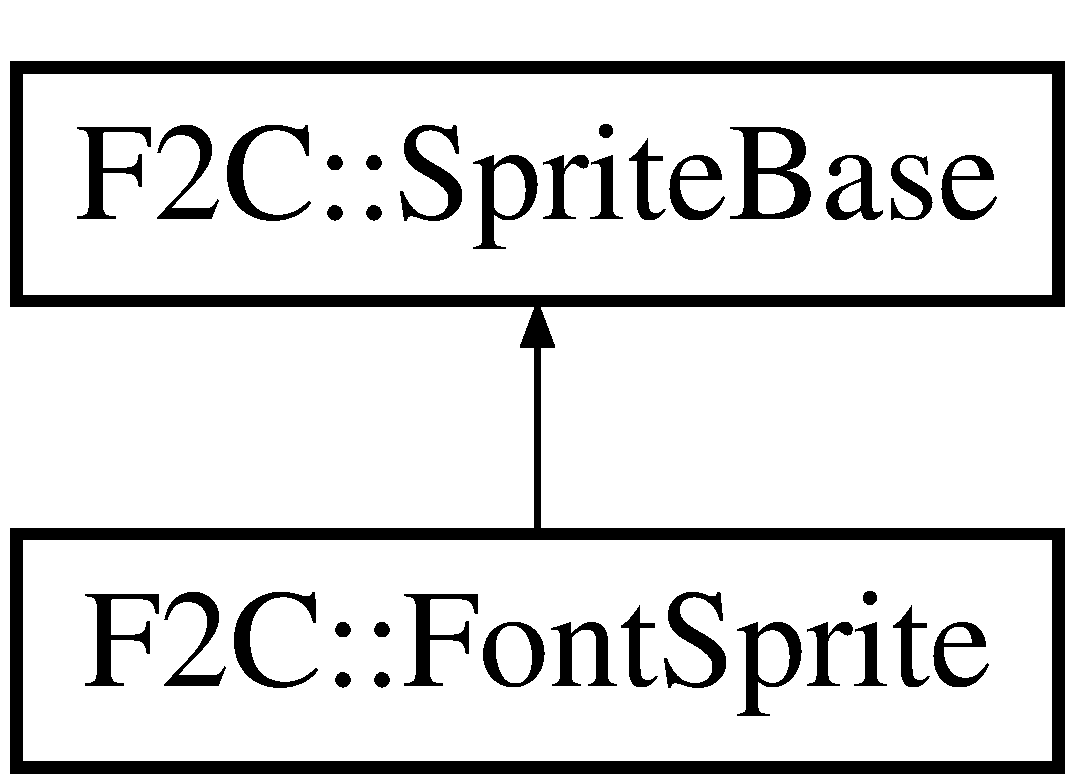
\includegraphics[height=2cm]{class_f2_c_1_1_font_sprite}
\end{center}
\end{figure}
\subsection*{Public Member Functions}
\begin{DoxyCompactItemize}
\item 
void \hyperlink{class_f2_c_1_1_font_sprite_ac6af1586ca99fd00365c1393f9a14817}{setViewport} (\hyperlink{class_f2_c_1_1_viewport}{Viewport} $\ast$\hyperlink{class_f2_c_1_1_font_sprite_a4f82be1613af7c8b83e5551ca6c81ed1}{viewport})
\begin{DoxyCompactList}\small\item\em setMethode: Set the pointer of the viewport and the clip\_\-rect. \item\end{DoxyCompactList}\item 
\hypertarget{class_f2_c_1_1_font_sprite_ab8375c3937eed4398ab1cfed98ca127b}{
\hyperlink{class_f2_c_1_1_font_sprite_ab8375c3937eed4398ab1cfed98ca127b}{FontSprite} ()}
\label{class_f2_c_1_1_font_sprite_ab8375c3937eed4398ab1cfed98ca127b}

\begin{DoxyCompactList}\small\item\em Default constructor. \item\end{DoxyCompactList}\item 
\hypertarget{class_f2_c_1_1_font_sprite_aa2310c7adcbabacdc4b840b54d8e4969}{
\hyperlink{class_f2_c_1_1_font_sprite_aa2310c7adcbabacdc4b840b54d8e4969}{FontSprite} (const \hyperlink{class_f2_c_1_1_font_sprite}{FontSprite} \&copy)}
\label{class_f2_c_1_1_font_sprite_aa2310c7adcbabacdc4b840b54d8e4969}

\begin{DoxyCompactList}\small\item\em Copy constructor. \item\end{DoxyCompactList}\item 
\hyperlink{class_f2_c_1_1_font_sprite_a7ce4fb660a3b32e3890807dae9b4e850}{FontSprite} (\hyperlink{class_f2_c_1_1_viewport}{Viewport} $\ast$\hyperlink{class_f2_c_1_1_font_sprite_a4f82be1613af7c8b83e5551ca6c81ed1}{viewport})
\begin{DoxyCompactList}\small\item\em Set the pointer of the viewport and the clip\_\-rect. \item\end{DoxyCompactList}\item 
\hypertarget{class_f2_c_1_1_font_sprite_ac7a37a9ada6207e49f7868dbec562ee5}{
\hyperlink{class_f2_c_1_1_font_sprite}{FontSprite} \& \hyperlink{class_f2_c_1_1_font_sprite_ac7a37a9ada6207e49f7868dbec562ee5}{operator=} (const \hyperlink{class_f2_c_1_1_font_sprite}{FontSprite} \&copy)}
\label{class_f2_c_1_1_font_sprite_ac7a37a9ada6207e49f7868dbec562ee5}

\begin{DoxyCompactList}\small\item\em Assignment operator with deep copy. \item\end{DoxyCompactList}\item 
\hyperlink{class_f2_c_1_1_font_sprite_a5c7ad536cebfee0660823bef1947e668}{FontSprite} (const \hyperlink{class_f2_c_1_1_bitmap}{Bitmap} $\ast$bitmapfont, \hyperlink{namespace_f2_c_a58be2bac9eb3e3c99cb41b6008bf4fae}{uint} charsperwidth=\hyperlink{class_f2_c_1_1_font_sprite_a4391313f8fd3a47ae2b9941d8540a098}{FontSprite::defaultCharsperW}, \hyperlink{namespace_f2_c_a58be2bac9eb3e3c99cb41b6008bf4fae}{uint} charsperheight=\hyperlink{class_f2_c_1_1_font_sprite_a2f7ed6629876bb340c5b3121d0c3a2b0}{FontSprite::defaultCharsperH})
\begin{DoxyCompactList}\small\item\em Load the pixels from the bitmap into the texture. If NULL, is equivalent to the behavior as a disabled texturing. \item\end{DoxyCompactList}\item 
void \hyperlink{class_f2_c_1_1_font_sprite_a36a224f59737fb06c4d79ee48b7e4068}{copyProperties} (const \hyperlink{class_f2_c_1_1_font_sprite}{FontSprite} \&copy)
\begin{DoxyCompactList}\small\item\em Copies all properties(x,y,z-\/Coord.,vColor,Texts,...), except the texture(\hyperlink{class_f2_c_1_1_bitmap}{Bitmap},bitmapWidth,Height,...). \item\end{DoxyCompactList}\item 
int \hyperlink{class_f2_c_1_1_font_sprite_a2c6fc77162983dc4d750258144410272}{render} () const 
\begin{DoxyCompactList}\small\item\em Render the text on the screen. \item\end{DoxyCompactList}\item 
void \hyperlink{class_f2_c_1_1_font_sprite_a067445bcf9a95c276413091161066cb1}{setBitmap} (const \hyperlink{class_f2_c_1_1_bitmap}{Bitmap} $\ast$bitmap, \hyperlink{namespace_f2_c_a58be2bac9eb3e3c99cb41b6008bf4fae}{uint} charsperwidth=\hyperlink{class_f2_c_1_1_font_sprite_a4391313f8fd3a47ae2b9941d8540a098}{FontSprite::defaultCharsperW}, \hyperlink{namespace_f2_c_a58be2bac9eb3e3c99cb41b6008bf4fae}{uint} charsperheight=\hyperlink{class_f2_c_1_1_font_sprite_a2f7ed6629876bb340c5b3121d0c3a2b0}{FontSprite::defaultCharsperH})
\begin{DoxyCompactList}\small\item\em Load the pixels from the bitmap into the texture. If NULL, is equivalent to the behavior as a disabled texturing. \item\end{DoxyCompactList}\item 
void \hyperlink{class_f2_c_1_1_font_sprite_ae1be1c6e70f794e6b8bf56b60528119e}{addText} (int \hyperlink{class_f2_c_1_1_sprite_base_a552f88034a04e6ac41f22519ac53076c}{x}, int \hyperlink{class_f2_c_1_1_sprite_base_a33a3d48628d9a3130c603eaf902f209f}{y}, \hyperlink{namespace_f2_c_a58be2bac9eb3e3c99cb41b6008bf4fae}{uint} width, \hyperlink{namespace_f2_c_a58be2bac9eb3e3c99cb41b6008bf4fae}{uint} height, std::string text)
\begin{DoxyCompactList}\small\item\em Adds a text to a specific position. \item\end{DoxyCompactList}\item 
void \hyperlink{class_f2_c_1_1_font_sprite_a86138fa37543cdf1c28735b175f55fb8}{addText} (const \hyperlink{class_f2_c_1_1_rect}{Rect} \&rect, std::string text)
\begin{DoxyCompactList}\small\item\em Adds a text to a specific position. \item\end{DoxyCompactList}\item 
\hypertarget{class_f2_c_1_1_font_sprite_ab293fd22588a8dbe63fb264ea8085e09}{
void \hyperlink{class_f2_c_1_1_font_sprite_ab293fd22588a8dbe63fb264ea8085e09}{clearTexts} ()}
\label{class_f2_c_1_1_font_sprite_ab293fd22588a8dbe63fb264ea8085e09}

\begin{DoxyCompactList}\small\item\em Clear all Texts. \item\end{DoxyCompactList}\item 
\hypertarget{class_f2_c_1_1_font_sprite_a81bce69eb04c048d007d98262e916824}{
\hyperlink{namespace_f2_c_a58be2bac9eb3e3c99cb41b6008bf4fae}{uint} \hyperlink{class_f2_c_1_1_font_sprite_a81bce69eb04c048d007d98262e916824}{getCharsperWidth} () const }
\label{class_f2_c_1_1_font_sprite_a81bce69eb04c048d007d98262e916824}

\begin{DoxyCompactList}\small\item\em getMethode: Characters per column \item\end{DoxyCompactList}\item 
\hypertarget{class_f2_c_1_1_font_sprite_abd03d3df667c51e99608a7e3cb7ba775}{
\hyperlink{namespace_f2_c_a58be2bac9eb3e3c99cb41b6008bf4fae}{uint} \hyperlink{class_f2_c_1_1_font_sprite_abd03d3df667c51e99608a7e3cb7ba775}{getCharsperHeight} () const }
\label{class_f2_c_1_1_font_sprite_abd03d3df667c51e99608a7e3cb7ba775}

\begin{DoxyCompactList}\small\item\em getMethode: Characters per line \item\end{DoxyCompactList}\item 
\hypertarget{class_f2_c_1_1_font_sprite_a3c086bec1f7abf0fc457b2499c69774a}{
const std::vector$<$ std::string $>$ \& \hyperlink{class_f2_c_1_1_font_sprite_a3c086bec1f7abf0fc457b2499c69774a}{getTexts} () const }
\label{class_f2_c_1_1_font_sprite_a3c086bec1f7abf0fc457b2499c69774a}

\begin{DoxyCompactList}\small\item\em getMethode: Inserted texts \item\end{DoxyCompactList}\item 
\hypertarget{class_f2_c_1_1_font_sprite_a38b3c9b85b6ec46d903a38b5619255c1}{
const std::vector$<$ \hyperlink{class_f2_c_1_1_rect}{Rect} $>$ \& \hyperlink{class_f2_c_1_1_font_sprite_a38b3c9b85b6ec46d903a38b5619255c1}{getTextsRect} () const }
\label{class_f2_c_1_1_font_sprite_a38b3c9b85b6ec46d903a38b5619255c1}

\begin{DoxyCompactList}\small\item\em getMethode: Size(in pixels) of inserted texts. \item\end{DoxyCompactList}\item 
\hypertarget{class_f2_c_1_1_font_sprite_a1beebb4264be624bafc96126bde7eeec}{
const \hyperlink{class_f2_c_1_1_rect}{Rect} $\ast$ \hyperlink{class_f2_c_1_1_font_sprite_a1beebb4264be624bafc96126bde7eeec}{getCharsRect} () const }
\label{class_f2_c_1_1_font_sprite_a1beebb4264be624bafc96126bde7eeec}

\begin{DoxyCompactList}\small\item\em getMethode: Return the coordinates and the size of all characters (ASCII :0-\/255, Size: 256). \item\end{DoxyCompactList}\end{DoxyCompactItemize}
\subsection*{Public Attributes}
\begin{DoxyCompactItemize}
\item 
\hypertarget{class_f2_c_1_1_font_sprite_a23c2acdd3cc212d56fcc9021744211d3}{
\hyperlink{class_f2_c_1_1_rect}{Rect} $\ast$ \hyperlink{class_f2_c_1_1_font_sprite_a23c2acdd3cc212d56fcc9021744211d3}{clip\_\-rect}}
\label{class_f2_c_1_1_font_sprite_a23c2acdd3cc212d56fcc9021744211d3}

\begin{DoxyCompactList}\small\item\em Clipping \hyperlink{class_f2_c_1_1_rect}{Rect}, Cutting the sprites on the screen the desired section or window. \item\end{DoxyCompactList}\item 
\hypertarget{class_f2_c_1_1_font_sprite_a4f82be1613af7c8b83e5551ca6c81ed1}{
\hyperlink{class_f2_c_1_1_viewport}{Viewport} $\ast$ \hyperlink{class_f2_c_1_1_font_sprite_a4f82be1613af7c8b83e5551ca6c81ed1}{viewport}}
\label{class_f2_c_1_1_font_sprite_a4f82be1613af7c8b83e5551ca6c81ed1}

\begin{DoxyCompactList}\small\item\em Additional Z-\/coordinate and \hyperlink{class_f2_c_1_1_color_tone}{ColorTone}. \item\end{DoxyCompactList}\item 
\hypertarget{class_f2_c_1_1_font_sprite_aefcc932827b98589b3ed922c1f01e678}{
\hyperlink{class_f2_c_1_1_color_tone}{ColorTone} \hyperlink{class_f2_c_1_1_font_sprite_aefcc932827b98589b3ed922c1f01e678}{tone}}
\label{class_f2_c_1_1_font_sprite_aefcc932827b98589b3ed922c1f01e678}

\begin{DoxyCompactList}\small\item\em \hyperlink{class_f2_c_1_1_color}{Color} tone. \item\end{DoxyCompactList}\item 
\hypertarget{class_f2_c_1_1_font_sprite_abf113caad3e684ea5ed58b6c1557147a}{
bool \hyperlink{class_f2_c_1_1_font_sprite_abf113caad3e684ea5ed58b6c1557147a}{italic}}
\label{class_f2_c_1_1_font_sprite_abf113caad3e684ea5ed58b6c1557147a}

\begin{DoxyCompactList}\small\item\em Sets the text to italics On/Off. \item\end{DoxyCompactList}\end{DoxyCompactItemize}
\subsection*{Static Public Attributes}
\begin{DoxyCompactItemize}
\item 
\hypertarget{class_f2_c_1_1_font_sprite_aed3db6661c90a9d48cfd76b0e77c9c98}{
static GLhandleARB \hyperlink{class_f2_c_1_1_font_sprite_aed3db6661c90a9d48cfd76b0e77c9c98}{ShaderProgramObj}}
\label{class_f2_c_1_1_font_sprite_aed3db6661c90a9d48cfd76b0e77c9c98}

\begin{DoxyCompactList}\small\item\em Handle by the ARB program object for the \hyperlink{class_f2_c_1_1_array_sprite}{ArraySprite}. (Default: NULL) \par
 The Tranzperenz(Alpha Color) of the generated shader image (with the ARB program object) can be determined by the grayscale. \item\end{DoxyCompactList}\item 
\hypertarget{class_f2_c_1_1_font_sprite_aba43429eee849af1fd7466f8a6e5291c}{
static \hyperlink{namespace_f2_c_1_1_tex_param_a64299c3972944468af4e8b0394c936c6}{TexParam::Tex\_\-Param} \hyperlink{class_f2_c_1_1_font_sprite_aba43429eee849af1fd7466f8a6e5291c}{filter}}
\label{class_f2_c_1_1_font_sprite_aba43429eee849af1fd7466f8a6e5291c}

\begin{DoxyCompactList}\small\item\em Set the texture filtering of the \hyperlink{class_f2_c_1_1_sprite}{Sprite}. (Default: Linear). \item\end{DoxyCompactList}\item 
\hypertarget{class_f2_c_1_1_font_sprite_a69244b901df9ec25c6a96e5a51dedb7e}{
static \hyperlink{namespace_f2_c_a711deb33697d145669b9c0c4fe87c7ca}{uint8} \hyperlink{class_f2_c_1_1_font_sprite_a69244b901df9ec25c6a96e5a51dedb7e}{AlphaTolerance}}
\label{class_f2_c_1_1_font_sprite_a69244b901df9ec25c6a96e5a51dedb7e}

\begin{DoxyCompactList}\small\item\em Transparency (alpha) tolerance, to determine the spacing between the Character (Is tolerance equal to 0: the whole rectangle of the Character. If the alpha value greater than or equal to the tolerance is measured as the distance from) (default: 1). \item\end{DoxyCompactList}\item 
\hypertarget{class_f2_c_1_1_font_sprite_a4391313f8fd3a47ae2b9941d8540a098}{
static \hyperlink{namespace_f2_c_a58be2bac9eb3e3c99cb41b6008bf4fae}{uint} \hyperlink{class_f2_c_1_1_font_sprite_a4391313f8fd3a47ae2b9941d8540a098}{defaultCharsperW}}
\label{class_f2_c_1_1_font_sprite_a4391313f8fd3a47ae2b9941d8540a098}

\begin{DoxyCompactList}\small\item\em Standard characters per column (default: 16). \item\end{DoxyCompactList}\item 
\hypertarget{class_f2_c_1_1_font_sprite_a2f7ed6629876bb340c5b3121d0c3a2b0}{
static \hyperlink{namespace_f2_c_a58be2bac9eb3e3c99cb41b6008bf4fae}{uint} \hyperlink{class_f2_c_1_1_font_sprite_a2f7ed6629876bb340c5b3121d0c3a2b0}{defaultCharsperH}}
\label{class_f2_c_1_1_font_sprite_a2f7ed6629876bb340c5b3121d0c3a2b0}

\begin{DoxyCompactList}\small\item\em Standard characters per line (default: 16). \item\end{DoxyCompactList}\end{DoxyCompactItemize}


\subsection{Detailed Description}
Displaying messages on the screen via BitmapFont (bitmap). Please note the following OpenGL capability are enabled when rendering and at the end disable: \par
 GL\_\-SCISSOR\_\-TEST \par
 GL\_\-STENCIL\_\-TEST \par
 GL\_\-TEXTURE\_\-2D \par
 GL\_\-DEPTH\_\-TEST \par
 GL\_\-ALPHA\_\-TEST \par
 GL\_\-BLEND \par
 and use glShadeModel(GL\_\-SMOOTH) \par
 \par
 Dont forget to set the depth and alpha test function, e.g.: \par
 glAlphaFunc(GL\_\-GREATER, 0.0f) \par
 glDepthFunc(GL\_\-LEQUAL) \par
 \par
 Used OpenGL Buffers \par
 -\/GL\_\-COLOR\_\-BUFFER\_\-BIT \par
 -\/GL\_\-DEPTH\_\-BUFFER\_\-BIT \par
 -\/GL\_\-STENCIL\_\-BUFFER\_\-BIT \par
 

\subsection{Constructor \& Destructor Documentation}
\hypertarget{class_f2_c_1_1_font_sprite_a7ce4fb660a3b32e3890807dae9b4e850}{
\index{F2C::FontSprite@{F2C::FontSprite}!FontSprite@{FontSprite}}
\index{FontSprite@{FontSprite}!F2C::FontSprite@{F2C::FontSprite}}
\subsubsection[{FontSprite}]{\setlength{\rightskip}{0pt plus 5cm}F2C::FontSprite::FontSprite ({\bf Viewport} $\ast$ {\em viewport})}}
\label{class_f2_c_1_1_font_sprite_a7ce4fb660a3b32e3890807dae9b4e850}


Set the pointer of the viewport and the clip\_\-rect. 
\begin{DoxyParams}{Parameters}
\item[{\em viewport}]Pointer of \hyperlink{class_f2_c_1_1_viewport}{Viewport} \end{DoxyParams}
\hypertarget{class_f2_c_1_1_font_sprite_a5c7ad536cebfee0660823bef1947e668}{
\index{F2C::FontSprite@{F2C::FontSprite}!FontSprite@{FontSprite}}
\index{FontSprite@{FontSprite}!F2C::FontSprite@{F2C::FontSprite}}
\subsubsection[{FontSprite}]{\setlength{\rightskip}{0pt plus 5cm}F2C::FontSprite::FontSprite (const {\bf Bitmap} $\ast$ {\em bitmapfont}, \/  {\bf uint} {\em charsperwidth} = {\ttfamily {\bf FontSprite::defaultCharsperW}}, \/  {\bf uint} {\em charsperheight} = {\ttfamily {\bf FontSprite::defaultCharsperH}})}}
\label{class_f2_c_1_1_font_sprite_a5c7ad536cebfee0660823bef1947e668}


Load the pixels from the bitmap into the texture. If NULL, is equivalent to the behavior as a disabled texturing. 
\begin{DoxyParams}{Parameters}
\item[{\em bitmapfont}]Pointer of \hyperlink{class_f2_c_1_1_bitmap}{Bitmap} \item[{\em charsperwidth}]Characters per column \item[{\em charsperheight}]Characters per line  \end{DoxyParams}


\subsection{Member Function Documentation}
\hypertarget{class_f2_c_1_1_font_sprite_a86138fa37543cdf1c28735b175f55fb8}{
\index{F2C::FontSprite@{F2C::FontSprite}!addText@{addText}}
\index{addText@{addText}!F2C::FontSprite@{F2C::FontSprite}}
\subsubsection[{addText}]{\setlength{\rightskip}{0pt plus 5cm}void F2C::FontSprite::addText (const {\bf Rect} \& {\em rect}, \/  std::string {\em text})}}
\label{class_f2_c_1_1_font_sprite_a86138fa37543cdf1c28735b175f55fb8}


Adds a text to a specific position. 
\begin{DoxyParams}{Parameters}
\item[{\em rect}]Display area \item[{\em text}]Text \end{DoxyParams}
\hypertarget{class_f2_c_1_1_font_sprite_ae1be1c6e70f794e6b8bf56b60528119e}{
\index{F2C::FontSprite@{F2C::FontSprite}!addText@{addText}}
\index{addText@{addText}!F2C::FontSprite@{F2C::FontSprite}}
\subsubsection[{addText}]{\setlength{\rightskip}{0pt plus 5cm}void F2C::FontSprite::addText (int {\em x}, \/  int {\em y}, \/  {\bf uint} {\em width}, \/  {\bf uint} {\em height}, \/  std::string {\em text})}}
\label{class_f2_c_1_1_font_sprite_ae1be1c6e70f794e6b8bf56b60528119e}


Adds a text to a specific position. 
\begin{DoxyParams}{Parameters}
\item[{\em x}]X coordinate \item[{\em y}]Y coordinate \item[{\em width}]Width of the display area \item[{\em height}]Height of the display area \item[{\em text}]Text \end{DoxyParams}
\hypertarget{class_f2_c_1_1_font_sprite_a36a224f59737fb06c4d79ee48b7e4068}{
\index{F2C::FontSprite@{F2C::FontSprite}!copyProperties@{copyProperties}}
\index{copyProperties@{copyProperties}!F2C::FontSprite@{F2C::FontSprite}}
\subsubsection[{copyProperties}]{\setlength{\rightskip}{0pt plus 5cm}void F2C::FontSprite::copyProperties (const {\bf FontSprite} \& {\em copy})}}
\label{class_f2_c_1_1_font_sprite_a36a224f59737fb06c4d79ee48b7e4068}


Copies all properties(x,y,z-\/Coord.,vColor,Texts,...), except the texture(\hyperlink{class_f2_c_1_1_bitmap}{Bitmap},bitmapWidth,Height,...). 
\begin{DoxyParams}{Parameters}
\item[{\em copy}]Source copy \end{DoxyParams}


Reimplemented from \hyperlink{class_f2_c_1_1_sprite_base_a8f7ea8a95a07688bfb2e6268a52b9215}{F2C::SpriteBase}.\hypertarget{class_f2_c_1_1_font_sprite_a2c6fc77162983dc4d750258144410272}{
\index{F2C::FontSprite@{F2C::FontSprite}!render@{render}}
\index{render@{render}!F2C::FontSprite@{F2C::FontSprite}}
\subsubsection[{render}]{\setlength{\rightskip}{0pt plus 5cm}int F2C::FontSprite::render () const\hspace{0.3cm}{\ttfamily  \mbox{[}virtual\mbox{]}}}}
\label{class_f2_c_1_1_font_sprite_a2c6fc77162983dc4d750258144410272}


Render the text on the screen. \begin{DoxyReturn}{Returns}
-\/1, show is false (or from viewport). 

-\/2, The width or height of the bitmap is 0. 

-\/3, There are no texts to display. 

-\/4, The alpha color of all 4 Vertices are less than 1. 

-\/5, zoom\_\-x or zoom\_\-y is exactly 0. 

1, Texts has been successfully rendered. 
\end{DoxyReturn}


Implements \hyperlink{class_f2_c_1_1_sprite_base_af9dfc70083ca5a774d3874b61a6f9abc}{F2C::SpriteBase}.\hypertarget{class_f2_c_1_1_font_sprite_a067445bcf9a95c276413091161066cb1}{
\index{F2C::FontSprite@{F2C::FontSprite}!setBitmap@{setBitmap}}
\index{setBitmap@{setBitmap}!F2C::FontSprite@{F2C::FontSprite}}
\subsubsection[{setBitmap}]{\setlength{\rightskip}{0pt plus 5cm}void F2C::FontSprite::setBitmap (const {\bf Bitmap} $\ast$ {\em bitmap}, \/  {\bf uint} {\em charsperwidth} = {\ttfamily {\bf FontSprite::defaultCharsperW}}, \/  {\bf uint} {\em charsperheight} = {\ttfamily {\bf FontSprite::defaultCharsperH}})}}
\label{class_f2_c_1_1_font_sprite_a067445bcf9a95c276413091161066cb1}


Load the pixels from the bitmap into the texture. If NULL, is equivalent to the behavior as a disabled texturing. 
\begin{DoxyParams}{Parameters}
\item[{\em bitmap}]Pointer of \hyperlink{class_f2_c_1_1_bitmap}{Bitmap} \item[{\em charsperwidth}]Characters per column \item[{\em charsperheight}]Characters per line  \end{DoxyParams}
\hypertarget{class_f2_c_1_1_font_sprite_ac6af1586ca99fd00365c1393f9a14817}{
\index{F2C::FontSprite@{F2C::FontSprite}!setViewport@{setViewport}}
\index{setViewport@{setViewport}!F2C::FontSprite@{F2C::FontSprite}}
\subsubsection[{setViewport}]{\setlength{\rightskip}{0pt plus 5cm}void F2C::FontSprite::setViewport ({\bf Viewport} $\ast$ {\em viewport})}}
\label{class_f2_c_1_1_font_sprite_ac6af1586ca99fd00365c1393f9a14817}


setMethode: Set the pointer of the viewport and the clip\_\-rect. 
\begin{DoxyParams}{Parameters}
\item[{\em viewport}]Pointer of \hyperlink{class_f2_c_1_1_viewport}{Viewport} \end{DoxyParams}

\hypertarget{class_f2_c_1_1_input}{
\section{F2C::Input Class Reference}
\label{class_f2_c_1_1_input}\index{F2C::Input@{F2C::Input}}
}


Singleton pattern: \hyperlink{class_f2_c_1_1_input}{Input} Handle from the keyboard, mouse, joystick and \hyperlink{class_f2_c_1_1_window}{Window}.  
\subsection*{Public Member Functions}
\begin{DoxyCompactItemize}
\item 
bool \hyperlink{class_f2_c_1_1_input_ad5c061a72547198cb6a3f5a1ce44298c}{InitInput} ()
\begin{DoxyCompactList}\small\item\em Initializes the input functions. \item\end{DoxyCompactList}\item 
\hypertarget{class_f2_c_1_1_input_a32e688e7274cd0536c6fb10a85216590}{
void \hyperlink{class_f2_c_1_1_input_a32e688e7274cd0536c6fb10a85216590}{update} ()}
\label{class_f2_c_1_1_input_a32e688e7274cd0536c6fb10a85216590}

\begin{DoxyCompactList}\small\item\em update \hyperlink{class_f2_c_1_1_input}{Input} Handle. \item\end{DoxyCompactList}\item 
void \hyperlink{class_f2_c_1_1_input_afe44e50d55a10eac43f4d114d01fcc9e}{getMousePos} (int $\ast$x, int $\ast$y)
\begin{DoxyCompactList}\small\item\em getMethode: Mouse position \item\end{DoxyCompactList}\item 
bool \hyperlink{class_f2_c_1_1_input_af3d14b1d81e6198c5e0fb5fccbdd0b5c}{getPressKey} (char ckey)
\begin{DoxyCompactList}\small\item\em getMethode: Pressed / released (also query for multiple keys simultaneously) \item\end{DoxyCompactList}\item 
bool \hyperlink{class_f2_c_1_1_input_a5684e139903d71e9a7a0ac6d209895a1}{getPressKey} (\hyperlink{namespace_f2_c_1_1_keyboard_event_a13172bec547dc5eb2eee6c4fcd64c486}{KeyboardEvent::Keyboard} key)
\begin{DoxyCompactList}\small\item\em getMethode: Pressed / released (also query for multiple keys simultaneously) \item\end{DoxyCompactList}\item 
bool \hyperlink{class_f2_c_1_1_input_a5fab8a63b42332d5da2c648654a93f82}{getRepeatKey} (char ckey)
\begin{DoxyCompactList}\small\item\em getMethode: Pressed / released (compulsive from RepeatMode) \item\end{DoxyCompactList}\item 
bool \hyperlink{class_f2_c_1_1_input_aba74013667f7cc0ea8d3b53de03262cd}{getRepeatKey} (\hyperlink{namespace_f2_c_1_1_keyboard_event_a13172bec547dc5eb2eee6c4fcd64c486}{KeyboardEvent::Keyboard} key)
\begin{DoxyCompactList}\small\item\em getMethode: Pressed / released (compulsive from RepeatMode) \item\end{DoxyCompactList}\item 
\hypertarget{class_f2_c_1_1_input_a033f3bf6ea0c0883b76af3fb9b7f0c05}{
const bool $\ast$ \hyperlink{class_f2_c_1_1_input_a033f3bf6ea0c0883b76af3fb9b7f0c05}{getRepeatKeyArray} ()}
\label{class_f2_c_1_1_input_a033f3bf6ea0c0883b76af3fb9b7f0c05}

\begin{DoxyCompactList}\small\item\em getMethode: Array of Repeat Keys (size: 319 = 256 (ASCII Chars) + 63 (Special Keys(ESC,Space,Enter,....)) ) \item\end{DoxyCompactList}\item 
\hypertarget{class_f2_c_1_1_input_a7a4c16d3b99c6c16ca32646db5b24586}{
const bool $\ast$ \hyperlink{class_f2_c_1_1_input_a7a4c16d3b99c6c16ca32646db5b24586}{getPressKeyArray} ()}
\label{class_f2_c_1_1_input_a7a4c16d3b99c6c16ca32646db5b24586}

\begin{DoxyCompactList}\small\item\em getMethode: Array of Pressed Keys (size: 319 = 256 (ASCII Chars) + 63 (Special Keys(ESC,Space,Enter,....)) ) \item\end{DoxyCompactList}\item 
\hypertarget{class_f2_c_1_1_input_a378b279161ad643dce3f7c5818343c29}{
size\_\-t \hyperlink{class_f2_c_1_1_input_a378b279161ad643dce3f7c5818343c29}{getSizeKeyArray} ()}
\label{class_f2_c_1_1_input_a378b279161ad643dce3f7c5818343c29}

\begin{DoxyCompactList}\small\item\em getMethode: Size of keyarray: 319 = 256 (ASCII Chars) + 63 (Special Keys(ESC,Space,Enter,....)) \item\end{DoxyCompactList}\item 
void \hyperlink{class_f2_c_1_1_input_a48e3b0a537bc1e49e3910021e8b4e299}{setRepeatMode} (bool on)
\begin{DoxyCompactList}\small\item\em setMethode: set Keyboard RepeatMode On/Off. If RepeatMode is on the pressed key is treated as rapidly pressed key. If RepeatMode is off the pressed key is treated as once pressed. \item\end{DoxyCompactList}\item 
\hypertarget{class_f2_c_1_1_input_a1fc788dab81fb6972b9825d6842ce245}{
bool \hyperlink{class_f2_c_1_1_input_a1fc788dab81fb6972b9825d6842ce245}{getRepeatMode} ()}
\label{class_f2_c_1_1_input_a1fc788dab81fb6972b9825d6842ce245}

\begin{DoxyCompactList}\small\item\em setMethode: Keyboard RepeatMode On/Off \item\end{DoxyCompactList}\item 
bool \hyperlink{class_f2_c_1_1_input_a9f6ddd6c1cb000651956d4778bf5ed11}{getPressMouse} (\hyperlink{namespace_f2_c_1_1_mouse_event_ad51c859ddf42f97a3c31fb60c21821a8}{MouseEvent::Mouse} mousekey)
\begin{DoxyCompactList}\small\item\em getMethode: Pressed / released \item\end{DoxyCompactList}\item 
\hypertarget{class_f2_c_1_1_input_ad5735b5ece3cb4647543261fdca31f25}{
int \hyperlink{class_f2_c_1_1_input_ad5735b5ece3cb4647543261fdca31f25}{getMouseWheel} ()}
\label{class_f2_c_1_1_input_ad5735b5ece3cb4647543261fdca31f25}

\begin{DoxyCompactList}\small\item\em getMethode: Mouse wheel position \item\end{DoxyCompactList}\item 
int \hyperlink{class_f2_c_1_1_input_ad2b10c018d3a0059dcfc7325de011d45}{getJoystickParam} (\hyperlink{namespace_f2_c_1_1_joystick_event_ada0230f460f765718db17ac021cbfc1f}{JoystickEvent::Joystick} joy, \hyperlink{namespace_f2_c_1_1_joystick_event_ae71fc0f92f6dd24cc1ffe1bd14b6ed82}{JoystickEvent::ParamJoystick} param)
\begin{DoxyCompactList}\small\item\em getMethode: Value of Joystick Param. \item\end{DoxyCompactList}\item 
int \hyperlink{class_f2_c_1_1_input_a4638b65b4be2c3c5254531b6e0e54a9b}{getJoystickPos} (\hyperlink{namespace_f2_c_1_1_joystick_event_ada0230f460f765718db17ac021cbfc1f}{JoystickEvent::Joystick} joy, float $\ast$pos, int numaxes)
\begin{DoxyCompactList}\small\item\em To get the current axis positions of the joystick. The position of an axis can be in the range -\/1.0 to 1.0, where positive values represent right, forward or up directions, while negative values represent left, back or down directions. If a requested axis is not supported by the joystick, the corresponding array element will be set to zero. The same goes for the situation when the joystick is not connected (all axes are treated as unsupported). \item\end{DoxyCompactList}\item 
int \hyperlink{class_f2_c_1_1_input_a1049f8515c9466de7635cc230bdd5a27}{getJoystickButtons} (\hyperlink{namespace_f2_c_1_1_joystick_event_ada0230f460f765718db17ac021cbfc1f}{JoystickEvent::Joystick} joy, \hyperlink{namespace_f2_c_a711deb33697d145669b9c0c4fe87c7ca}{uint8} $\ast$buttons, int numbuttons)
\begin{DoxyCompactList}\small\item\em To get the current buttonsof the joystick. the buttons argument can be either 1 or 0, telling if the corresponding button is currently held down or not. Unsupported buttons will have the value 0. \item\end{DoxyCompactList}\item 
void \hyperlink{class_f2_c_1_1_input_a04fd09840025c2d60e483a1d0127255b}{setMousePos} (int x, int y)
\begin{DoxyCompactList}\small\item\em setMethode: Set mouse position. \item\end{DoxyCompactList}\item 
void \hyperlink{class_f2_c_1_1_input_ab28d56430cadbe95356fd30ca5abead6}{setMouseWheel} (int pos)
\begin{DoxyCompactList}\small\item\em setMethode: Set mouse wheel position \item\end{DoxyCompactList}\end{DoxyCompactItemize}
\subsection*{Static Public Member Functions}
\begin{DoxyCompactItemize}
\item 
\hypertarget{class_f2_c_1_1_input_a8fee4ef6592b8bac70d960f35bfddd15}{
static \hyperlink{class_f2_c_1_1_input}{Input} $\ast$ \hyperlink{class_f2_c_1_1_input_a8fee4ef6592b8bac70d960f35bfddd15}{getInstance} ()}
\label{class_f2_c_1_1_input_a8fee4ef6592b8bac70d960f35bfddd15}

\begin{DoxyCompactList}\small\item\em getmethode: Instance \item\end{DoxyCompactList}\end{DoxyCompactItemize}


\subsection{Detailed Description}
Singleton pattern: \hyperlink{class_f2_c_1_1_input}{Input} Handle from the keyboard, mouse, joystick and \hyperlink{class_f2_c_1_1_window}{Window}. 

\subsection{Member Function Documentation}
\hypertarget{class_f2_c_1_1_input_a1049f8515c9466de7635cc230bdd5a27}{
\index{F2C::Input@{F2C::Input}!getJoystickButtons@{getJoystickButtons}}
\index{getJoystickButtons@{getJoystickButtons}!F2C::Input@{F2C::Input}}
\subsubsection[{getJoystickButtons}]{\setlength{\rightskip}{0pt plus 5cm}int F2C::Input::getJoystickButtons ({\bf JoystickEvent::Joystick} {\em joy}, \/  {\bf uint8} $\ast$ {\em buttons}, \/  int {\em numbuttons})}}
\label{class_f2_c_1_1_input_a1049f8515c9466de7635cc230bdd5a27}


To get the current buttonsof the joystick. the buttons argument can be either 1 or 0, telling if the corresponding button is currently held down or not. Unsupported buttons will have the value 0. 
\begin{DoxyParams}{Parameters}
\item[{\em joy}]Joystick nummer \item[{\em buttons}]Target reference variable: Array in which all the buttons. \item[{\em numbuttons}]Gibt an, wie viele tasten zurueckgegeben werden. \end{DoxyParams}
\begin{DoxyReturn}{Returns}
returns the state of joystick buttons instead of axis positions. 
\end{DoxyReturn}
\hypertarget{class_f2_c_1_1_input_ad2b10c018d3a0059dcfc7325de011d45}{
\index{F2C::Input@{F2C::Input}!getJoystickParam@{getJoystickParam}}
\index{getJoystickParam@{getJoystickParam}!F2C::Input@{F2C::Input}}
\subsubsection[{getJoystickParam}]{\setlength{\rightskip}{0pt plus 5cm}int F2C::Input::getJoystickParam ({\bf JoystickEvent::Joystick} {\em joy}, \/  {\bf JoystickEvent::ParamJoystick} {\em param})}}
\label{class_f2_c_1_1_input_ad2b10c018d3a0059dcfc7325de011d45}


getMethode: Value of Joystick Param. 
\begin{DoxyParams}{Parameters}
\item[{\em joy}]Joystick nummer \item[{\em param}]Joystick Param \end{DoxyParams}
\hypertarget{class_f2_c_1_1_input_a4638b65b4be2c3c5254531b6e0e54a9b}{
\index{F2C::Input@{F2C::Input}!getJoystickPos@{getJoystickPos}}
\index{getJoystickPos@{getJoystickPos}!F2C::Input@{F2C::Input}}
\subsubsection[{getJoystickPos}]{\setlength{\rightskip}{0pt plus 5cm}int F2C::Input::getJoystickPos ({\bf JoystickEvent::Joystick} {\em joy}, \/  float $\ast$ {\em pos}, \/  int {\em numaxes})}}
\label{class_f2_c_1_1_input_a4638b65b4be2c3c5254531b6e0e54a9b}


To get the current axis positions of the joystick. The position of an axis can be in the range -\/1.0 to 1.0, where positive values represent right, forward or up directions, while negative values represent left, back or down directions. If a requested axis is not supported by the joystick, the corresponding array element will be set to zero. The same goes for the situation when the joystick is not connected (all axes are treated as unsupported). 
\begin{DoxyParams}{Parameters}
\item[{\em joy}]Joystick nummer \item[{\em pos}]Target reference variable: Array in which all the axis positions. \item[{\em numaxes}]Numbers of axes \end{DoxyParams}
\begin{DoxyReturn}{Returns}
returns the actual number of axes that were returned, which could be less than numaxes if the joystick does not support all the requested axes, or if the joystick is not connected. 
\end{DoxyReturn}
\hypertarget{class_f2_c_1_1_input_afe44e50d55a10eac43f4d114d01fcc9e}{
\index{F2C::Input@{F2C::Input}!getMousePos@{getMousePos}}
\index{getMousePos@{getMousePos}!F2C::Input@{F2C::Input}}
\subsubsection[{getMousePos}]{\setlength{\rightskip}{0pt plus 5cm}void F2C::Input::getMousePos (int $\ast$ {\em x}, \/  int $\ast$ {\em y})}}
\label{class_f2_c_1_1_input_afe44e50d55a10eac43f4d114d01fcc9e}


getMethode: Mouse position 
\begin{DoxyParams}{Parameters}
\item[{\em x}]Target reference variable: X-\/Coordinate \item[{\em y}]Target reference variable: Y-\/Coordinate \end{DoxyParams}
\hypertarget{class_f2_c_1_1_input_a5684e139903d71e9a7a0ac6d209895a1}{
\index{F2C::Input@{F2C::Input}!getPressKey@{getPressKey}}
\index{getPressKey@{getPressKey}!F2C::Input@{F2C::Input}}
\subsubsection[{getPressKey}]{\setlength{\rightskip}{0pt plus 5cm}bool F2C::Input::getPressKey ({\bf KeyboardEvent::Keyboard} {\em key})}}
\label{class_f2_c_1_1_input_a5684e139903d71e9a7a0ac6d209895a1}


getMethode: Pressed / released (also query for multiple keys simultaneously) 
\begin{DoxyParams}{Parameters}
\item[{\em key}]Special Button \end{DoxyParams}
\hypertarget{class_f2_c_1_1_input_af3d14b1d81e6198c5e0fb5fccbdd0b5c}{
\index{F2C::Input@{F2C::Input}!getPressKey@{getPressKey}}
\index{getPressKey@{getPressKey}!F2C::Input@{F2C::Input}}
\subsubsection[{getPressKey}]{\setlength{\rightskip}{0pt plus 5cm}bool F2C::Input::getPressKey (char {\em ckey})}}
\label{class_f2_c_1_1_input_af3d14b1d81e6198c5e0fb5fccbdd0b5c}


getMethode: Pressed / released (also query for multiple keys simultaneously) 
\begin{DoxyParams}{Parameters}
\item[{\em ckey}]Character \end{DoxyParams}
\hypertarget{class_f2_c_1_1_input_a9f6ddd6c1cb000651956d4778bf5ed11}{
\index{F2C::Input@{F2C::Input}!getPressMouse@{getPressMouse}}
\index{getPressMouse@{getPressMouse}!F2C::Input@{F2C::Input}}
\subsubsection[{getPressMouse}]{\setlength{\rightskip}{0pt plus 5cm}bool F2C::Input::getPressMouse ({\bf MouseEvent::Mouse} {\em mousekey})}}
\label{class_f2_c_1_1_input_a9f6ddd6c1cb000651956d4778bf5ed11}


getMethode: Pressed / released 
\begin{DoxyParams}{Parameters}
\item[{\em mousekey}]Mouse button \end{DoxyParams}
\hypertarget{class_f2_c_1_1_input_aba74013667f7cc0ea8d3b53de03262cd}{
\index{F2C::Input@{F2C::Input}!getRepeatKey@{getRepeatKey}}
\index{getRepeatKey@{getRepeatKey}!F2C::Input@{F2C::Input}}
\subsubsection[{getRepeatKey}]{\setlength{\rightskip}{0pt plus 5cm}bool F2C::Input::getRepeatKey ({\bf KeyboardEvent::Keyboard} {\em key})}}
\label{class_f2_c_1_1_input_aba74013667f7cc0ea8d3b53de03262cd}


getMethode: Pressed / released (compulsive from RepeatMode) 
\begin{DoxyParams}{Parameters}
\item[{\em key}]Special Button \end{DoxyParams}
\hypertarget{class_f2_c_1_1_input_a5fab8a63b42332d5da2c648654a93f82}{
\index{F2C::Input@{F2C::Input}!getRepeatKey@{getRepeatKey}}
\index{getRepeatKey@{getRepeatKey}!F2C::Input@{F2C::Input}}
\subsubsection[{getRepeatKey}]{\setlength{\rightskip}{0pt plus 5cm}bool F2C::Input::getRepeatKey (char {\em ckey})}}
\label{class_f2_c_1_1_input_a5fab8a63b42332d5da2c648654a93f82}


getMethode: Pressed / released (compulsive from RepeatMode) 
\begin{DoxyParams}{Parameters}
\item[{\em ckey}]Character \end{DoxyParams}
\hypertarget{class_f2_c_1_1_input_ad5c061a72547198cb6a3f5a1ce44298c}{
\index{F2C::Input@{F2C::Input}!InitInput@{InitInput}}
\index{InitInput@{InitInput}!F2C::Input@{F2C::Input}}
\subsubsection[{InitInput}]{\setlength{\rightskip}{0pt plus 5cm}bool F2C::Input::InitInput ()}}
\label{class_f2_c_1_1_input_ad5c061a72547198cb6a3f5a1ce44298c}


Initializes the input functions. \begin{DoxyReturn}{Returns}
Success / failure 
\end{DoxyReturn}
\hypertarget{class_f2_c_1_1_input_a04fd09840025c2d60e483a1d0127255b}{
\index{F2C::Input@{F2C::Input}!setMousePos@{setMousePos}}
\index{setMousePos@{setMousePos}!F2C::Input@{F2C::Input}}
\subsubsection[{setMousePos}]{\setlength{\rightskip}{0pt plus 5cm}void F2C::Input::setMousePos (int {\em x}, \/  int {\em y})}}
\label{class_f2_c_1_1_input_a04fd09840025c2d60e483a1d0127255b}


setMethode: Set mouse position. 
\begin{DoxyParams}{Parameters}
\item[{\em x}]X-\/Coordinate \item[{\em y}]X-\/Coordinate \end{DoxyParams}
\hypertarget{class_f2_c_1_1_input_ab28d56430cadbe95356fd30ca5abead6}{
\index{F2C::Input@{F2C::Input}!setMouseWheel@{setMouseWheel}}
\index{setMouseWheel@{setMouseWheel}!F2C::Input@{F2C::Input}}
\subsubsection[{setMouseWheel}]{\setlength{\rightskip}{0pt plus 5cm}void F2C::Input::setMouseWheel (int {\em pos})}}
\label{class_f2_c_1_1_input_ab28d56430cadbe95356fd30ca5abead6}


setMethode: Set mouse wheel position 
\begin{DoxyParams}{Parameters}
\item[{\em pos}]Mouse wheel position \end{DoxyParams}
\hypertarget{class_f2_c_1_1_input_a48e3b0a537bc1e49e3910021e8b4e299}{
\index{F2C::Input@{F2C::Input}!setRepeatMode@{setRepeatMode}}
\index{setRepeatMode@{setRepeatMode}!F2C::Input@{F2C::Input}}
\subsubsection[{setRepeatMode}]{\setlength{\rightskip}{0pt plus 5cm}void F2C::Input::setRepeatMode (bool {\em on})}}
\label{class_f2_c_1_1_input_a48e3b0a537bc1e49e3910021e8b4e299}


setMethode: set Keyboard RepeatMode On/Off. If RepeatMode is on the pressed key is treated as rapidly pressed key. If RepeatMode is off the pressed key is treated as once pressed. 
\begin{DoxyParams}{Parameters}
\item[{\em on}]RepeatMode \end{DoxyParams}

\hypertarget{class_f2_c_1_1_log_error}{
\section{F2C::LogError Class Reference}
\label{class_f2_c_1_1_log_error}\index{F2C::LogError@{F2C::LogError}}
}


Writing log files and exception handler.  


\subsection*{Classes}
\begin{DoxyCompactItemize}
\item 
class {\bfseries LEError}
\end{DoxyCompactItemize}
\subsection*{Public Member Functions}
\begin{DoxyCompactItemize}
\item 
\hypertarget{class_f2_c_1_1_log_error_a119ab8a21960a4b7a6dbd4ddce334e5f}{
void \hyperlink{class_f2_c_1_1_log_error_a119ab8a21960a4b7a6dbd4ddce334e5f}{writeError} ()}
\label{class_f2_c_1_1_log_error_a119ab8a21960a4b7a6dbd4ddce334e5f}

\begin{DoxyCompactList}\small\item\em Creates and writes the log file. \item\end{DoxyCompactList}\item 
void \hyperlink{class_f2_c_1_1_log_error_abce3f1efd9a5b93e1bd400f743ba398e}{setError} (std::string file, std::string func, \hyperlink{namespace_f2_c_a58be2bac9eb3e3c99cb41b6008bf4fae}{uint} line, std::string string)
\begin{DoxyCompactList}\small\item\em Sets the filename, line, function, and the Log text. \item\end{DoxyCompactList}\item 
void \hyperlink{class_f2_c_1_1_log_error_a37013f16d6418b8881c8df0be43909c6}{setError} (std::string file, std::string func, \hyperlink{namespace_f2_c_a58be2bac9eb3e3c99cb41b6008bf4fae}{uint} line, void $\ast$ptr, std::string string)
\begin{DoxyCompactList}\small\item\em Sets the file name, line, function, and the Log text and the adress. \item\end{DoxyCompactList}\item 
\hypertarget{class_f2_c_1_1_log_error_a48e68471f785fe0a6482c825dcfa15d0}{
std::string \hyperlink{class_f2_c_1_1_log_error_a48e68471f785fe0a6482c825dcfa15d0}{getError} () const }
\label{class_f2_c_1_1_log_error_a48e68471f785fe0a6482c825dcfa15d0}

\begin{DoxyCompactList}\small\item\em getMethode: Log text \item\end{DoxyCompactList}\item 
void \hyperlink{class_f2_c_1_1_log_error_ac571b7a599761f5ed869832b023a3d92}{setError} (std::string string)
\begin{DoxyCompactList}\small\item\em setMethode: Set the Log text \item\end{DoxyCompactList}\end{DoxyCompactItemize}
\subsection*{Static Public Member Functions}
\begin{DoxyCompactItemize}
\item 
\hypertarget{class_f2_c_1_1_log_error_a37fe6ce832fff15978a84a923b081b1b}{
static void \hyperlink{class_f2_c_1_1_log_error_a37fe6ce832fff15978a84a923b081b1b}{ClearLog} ()}
\label{class_f2_c_1_1_log_error_a37fe6ce832fff15978a84a923b081b1b}

\begin{DoxyCompactList}\small\item\em Clears the text in the Log file. \item\end{DoxyCompactList}\item 
static void \hyperlink{class_f2_c_1_1_log_error_a7821ec372e85a3d2c7095c4902525908}{writeString} (std::string string)
\begin{DoxyCompactList}\small\item\em Writes a text into the Log text. \item\end{DoxyCompactList}\item 
\hypertarget{class_f2_c_1_1_log_error_ac1645d431457463e0396b46d556ab88c}{
static std::string \hyperlink{class_f2_c_1_1_log_error_ac1645d431457463e0396b46d556ab88c}{getOpenGLError} ()}
\label{class_f2_c_1_1_log_error_ac1645d431457463e0396b46d556ab88c}

\begin{DoxyCompactList}\small\item\em getMethode: OpenGL Error \item\end{DoxyCompactList}\end{DoxyCompactItemize}
\subsection*{Static Public Attributes}
\begin{DoxyCompactItemize}
\item 
static std::string \hyperlink{class_f2_c_1_1_log_error_aa5dc474b29884812c02be68e1c45c56e}{filename}
\begin{DoxyCompactList}\small\item\em Default destructor. \item\end{DoxyCompactList}\item 
\hypertarget{class_f2_c_1_1_log_error_a40a853a8ce671575d7b57433b14d2789}{
static bool \hyperlink{class_f2_c_1_1_log_error_a40a853a8ce671575d7b57433b14d2789}{writelog}}
\label{class_f2_c_1_1_log_error_a40a853a8ce671575d7b57433b14d2789}

\begin{DoxyCompactList}\small\item\em Logfile write allowed/forbidden (default: true). \item\end{DoxyCompactList}\end{DoxyCompactItemize}
\subsection*{Friends}
\begin{DoxyCompactItemize}
\item 
std::ostream \& \hyperlink{class_f2_c_1_1_log_error_a572bf2fc9d5712eecbab42ba4f0fe3b3}{operator$<$$<$} (std::ostream \&out, const \hyperlink{class_f2_c_1_1_log_error}{LogError} \&obj)
\begin{DoxyCompactList}\small\item\em Write the Object into output stream. (dont write pointer (\hyperlink{class_f2_c_1_1_viewport}{Viewport},clip\_\-rect)). \item\end{DoxyCompactList}\item 
std::istream \& \hyperlink{class_f2_c_1_1_log_error_a6fcf2a3199b92518fa70d937aea78aed}{operator$>$$>$} (std::istream \&in, \hyperlink{class_f2_c_1_1_log_error}{LogError} \&obj)
\begin{DoxyCompactList}\small\item\em Read the Object from input stream. (dont read pointer (\hyperlink{class_f2_c_1_1_viewport}{Viewport},clip\_\-rect)). \item\end{DoxyCompactList}\end{DoxyCompactItemize}


\subsection{Detailed Description}
Writing log files and exception handler. \par
 
\begin{DoxyCode}
 #define SETLOGERROR(error,string) error.setError(__FILE__,__FUNCTION__,__LINE__,
      string) 
\end{DoxyCode}
 Sets the filename, line, and the function name. \par
 
\begin{DoxyCode}
 #define P_SETLOGERROR(error,pointer,string) error.setError(__FILE__,__FUNCTION__
      ,__LINE__,pointer,string) 
\end{DoxyCode}
 Sets the filename, line, function name, and the address. 

\subsection{Member Function Documentation}
\hypertarget{class_f2_c_1_1_log_error_abce3f1efd9a5b93e1bd400f743ba398e}{
\index{F2C::LogError@{F2C::LogError}!setError@{setError}}
\index{setError@{setError}!F2C::LogError@{F2C::LogError}}
\subsubsection[{setError}]{\setlength{\rightskip}{0pt plus 5cm}void F2C::LogError::setError (
\begin{DoxyParamCaption}
\item[{std::string}]{ file, }
\item[{std::string}]{ func, }
\item[{{\bf uint}}]{ line, }
\item[{std::string}]{ string}
\end{DoxyParamCaption}
)}}
\label{class_f2_c_1_1_log_error_abce3f1efd9a5b93e1bd400f743ba398e}


Sets the filename, line, function, and the Log text. 


\begin{DoxyParams}{Parameters}
\item[{\em file}]Filename \item[{\em func}]Function name \item[{\em line}]Line \item[{\em string}]Text \end{DoxyParams}
\hypertarget{class_f2_c_1_1_log_error_ac571b7a599761f5ed869832b023a3d92}{
\index{F2C::LogError@{F2C::LogError}!setError@{setError}}
\index{setError@{setError}!F2C::LogError@{F2C::LogError}}
\subsubsection[{setError}]{\setlength{\rightskip}{0pt plus 5cm}void F2C::LogError::setError (
\begin{DoxyParamCaption}
\item[{std::string}]{ string}
\end{DoxyParamCaption}
)}}
\label{class_f2_c_1_1_log_error_ac571b7a599761f5ed869832b023a3d92}


setMethode: Set the Log text 


\begin{DoxyParams}{Parameters}
\item[{\em string}]LogFile Text \end{DoxyParams}
\hypertarget{class_f2_c_1_1_log_error_a37013f16d6418b8881c8df0be43909c6}{
\index{F2C::LogError@{F2C::LogError}!setError@{setError}}
\index{setError@{setError}!F2C::LogError@{F2C::LogError}}
\subsubsection[{setError}]{\setlength{\rightskip}{0pt plus 5cm}void F2C::LogError::setError (
\begin{DoxyParamCaption}
\item[{std::string}]{ file, }
\item[{std::string}]{ func, }
\item[{{\bf uint}}]{ line, }
\item[{void $\ast$}]{ ptr, }
\item[{std::string}]{ string}
\end{DoxyParamCaption}
)}}
\label{class_f2_c_1_1_log_error_a37013f16d6418b8881c8df0be43909c6}


Sets the file name, line, function, and the Log text and the adress. 


\begin{DoxyParams}{Parameters}
\item[{\em file}]Filename \item[{\em func}]Function name \item[{\em line}]line \item[{\em ptr}]Adress \item[{\em string}]Text \end{DoxyParams}
\hypertarget{class_f2_c_1_1_log_error_a7821ec372e85a3d2c7095c4902525908}{
\index{F2C::LogError@{F2C::LogError}!writeString@{writeString}}
\index{writeString@{writeString}!F2C::LogError@{F2C::LogError}}
\subsubsection[{writeString}]{\setlength{\rightskip}{0pt plus 5cm}static void F2C::LogError::writeString (
\begin{DoxyParamCaption}
\item[{std::string}]{ string}
\end{DoxyParamCaption}
)\hspace{0.3cm}{\ttfamily  \mbox{[}static\mbox{]}}}}
\label{class_f2_c_1_1_log_error_a7821ec372e85a3d2c7095c4902525908}


Writes a text into the Log text. 


\begin{DoxyParams}{Parameters}
\item[{\em string}]Text \end{DoxyParams}


\subsection{Friends And Related Function Documentation}
\hypertarget{class_f2_c_1_1_log_error_a572bf2fc9d5712eecbab42ba4f0fe3b3}{
\index{F2C::LogError@{F2C::LogError}!operator$<$$<$@{operator$<$$<$}}
\index{operator$<$$<$@{operator$<$$<$}!F2C::LogError@{F2C::LogError}}
\subsubsection[{operator$<$$<$}]{\setlength{\rightskip}{0pt plus 5cm}std::ostream\& operator$<$$<$ (
\begin{DoxyParamCaption}
\item[{std::ostream \&}]{ out, }
\item[{const {\bf LogError} \&}]{ obj}
\end{DoxyParamCaption}
)\hspace{0.3cm}{\ttfamily  \mbox{[}friend\mbox{]}}}}
\label{class_f2_c_1_1_log_error_a572bf2fc9d5712eecbab42ba4f0fe3b3}


Write the Object into output stream. (dont write pointer (\hyperlink{class_f2_c_1_1_viewport}{Viewport},clip\_\-rect)). 


\begin{DoxyParams}{Parameters}
\item[{\em out}]Output stream \item[{\em obj}]Object \end{DoxyParams}
\hypertarget{class_f2_c_1_1_log_error_a6fcf2a3199b92518fa70d937aea78aed}{
\index{F2C::LogError@{F2C::LogError}!operator$>$$>$@{operator$>$$>$}}
\index{operator$>$$>$@{operator$>$$>$}!F2C::LogError@{F2C::LogError}}
\subsubsection[{operator$>$$>$}]{\setlength{\rightskip}{0pt plus 5cm}std::istream\& operator$>$$>$ (
\begin{DoxyParamCaption}
\item[{std::istream \&}]{ in, }
\item[{{\bf LogError} \&}]{ obj}
\end{DoxyParamCaption}
)\hspace{0.3cm}{\ttfamily  \mbox{[}friend\mbox{]}}}}
\label{class_f2_c_1_1_log_error_a6fcf2a3199b92518fa70d937aea78aed}


Read the Object from input stream. (dont read pointer (\hyperlink{class_f2_c_1_1_viewport}{Viewport},clip\_\-rect)). 


\begin{DoxyParams}{Parameters}
\item[{\em in}]\hyperlink{class_f2_c_1_1_input}{Input} stream \item[{\em obj}]Object \end{DoxyParams}


\subsection{Member Data Documentation}
\hypertarget{class_f2_c_1_1_log_error_aa5dc474b29884812c02be68e1c45c56e}{
\index{F2C::LogError@{F2C::LogError}!filename@{filename}}
\index{filename@{filename}!F2C::LogError@{F2C::LogError}}
\subsubsection[{filename}]{\setlength{\rightskip}{0pt plus 5cm}std::string {\bf F2C::LogError::filename}\hspace{0.3cm}{\ttfamily  \mbox{[}static\mbox{]}}}}
\label{class_f2_c_1_1_log_error_aa5dc474b29884812c02be68e1c45c56e}


Default destructor. 

Log file name (default: logfile) 
\hypertarget{class_f2_c_1_1_plane}{
\section{F2C::Plane Class Reference}
\label{class_f2_c_1_1_plane}\index{F2C::Plane@{F2C::Plane}}
}


Renders an image (\hyperlink{class_f2_c_1_1_bitmap}{Bitmap} class) on the screen as an infinite Scrollable image.  


Inheritance diagram for F2C::Plane:\begin{figure}[H]
\begin{center}
\leavevmode
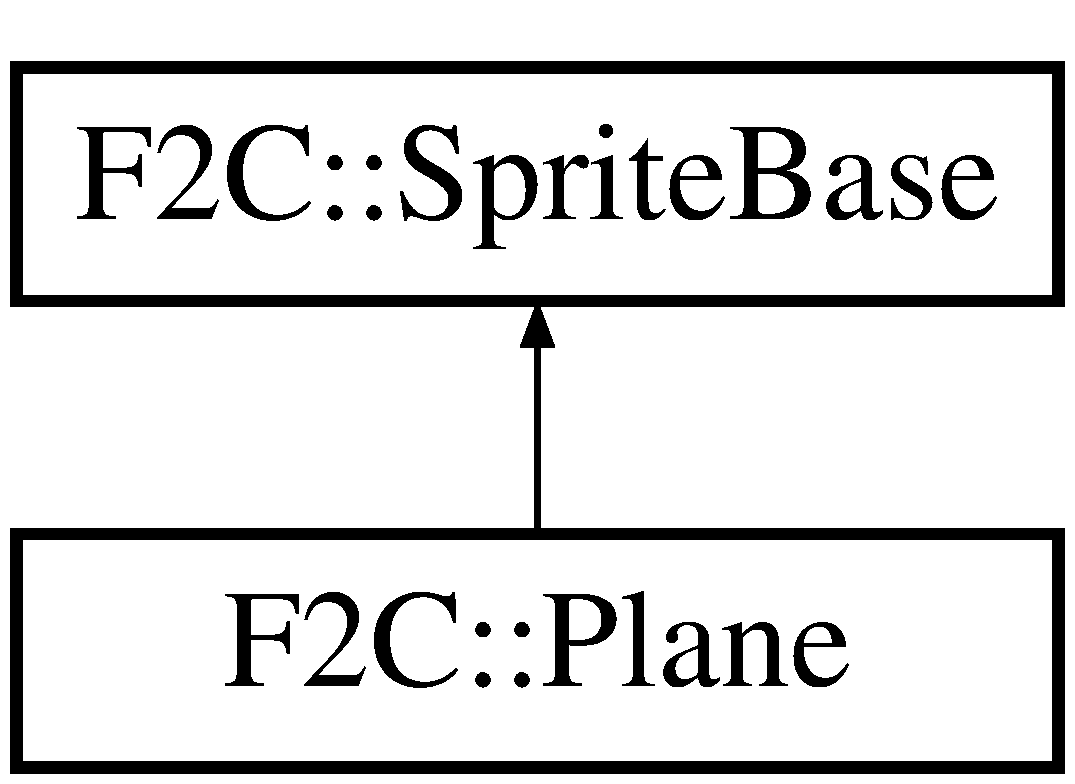
\includegraphics[height=2.000000cm]{class_f2_c_1_1_plane}
\end{center}
\end{figure}
\subsection*{Public Member Functions}
\begin{DoxyCompactItemize}
\item 
\hypertarget{class_f2_c_1_1_plane_ae964dce807d325a229b2b0483d04bac0}{
\hyperlink{class_f2_c_1_1_plane_ae964dce807d325a229b2b0483d04bac0}{Plane} ()}
\label{class_f2_c_1_1_plane_ae964dce807d325a229b2b0483d04bac0}

\begin{DoxyCompactList}\small\item\em Default constructor. \item\end{DoxyCompactList}\item 
\hyperlink{class_f2_c_1_1_plane_a257596b463548284ec5699e5290b4a9d}{Plane} (\hyperlink{class_f2_c_1_1_viewport}{Viewport} $\ast$\hyperlink{class_f2_c_1_1_plane_a755aaa0644174adc1574d04a1378c22f}{viewport})
\begin{DoxyCompactList}\small\item\em Set the pointer of the viewport and the clip\_\-rect. \item\end{DoxyCompactList}\item 
\hyperlink{class_f2_c_1_1_plane_a2d6c6add986f779ce1879a4ac4ad5458}{Plane} (const \hyperlink{class_f2_c_1_1_bitmap}{Bitmap} $\ast$bitmap)
\begin{DoxyCompactList}\small\item\em Load the pixels from the bitmap into the texture. If NULL, is equivalent to the behavior as a disabled texturing. \item\end{DoxyCompactList}\item 
\hypertarget{class_f2_c_1_1_plane_a6d692311afad34bbd0407ecffa8fda6e}{
\hyperlink{class_f2_c_1_1_plane_a6d692311afad34bbd0407ecffa8fda6e}{Plane} (const \hyperlink{class_f2_c_1_1_plane}{Plane} \&copy)}
\label{class_f2_c_1_1_plane_a6d692311afad34bbd0407ecffa8fda6e}

\begin{DoxyCompactList}\small\item\em Copy constructor. \item\end{DoxyCompactList}\item 
\hypertarget{class_f2_c_1_1_plane_afb63aaf92522d735b7614d2ccbda4e99}{
\hyperlink{class_f2_c_1_1_plane}{Plane} \& \hyperlink{class_f2_c_1_1_plane_afb63aaf92522d735b7614d2ccbda4e99}{operator=} (const \hyperlink{class_f2_c_1_1_plane}{Plane} \&copy)}
\label{class_f2_c_1_1_plane_afb63aaf92522d735b7614d2ccbda4e99}

\begin{DoxyCompactList}\small\item\em Assignment operator with deep copy. \item\end{DoxyCompactList}\item 
void \hyperlink{class_f2_c_1_1_plane_ac3ee4529b515cc641b6e9b27d76fc2ef}{copyProperties} (const \hyperlink{class_f2_c_1_1_plane}{Plane} \&copy)
\begin{DoxyCompactList}\small\item\em Copies all properties(x,y,z-\/Coord.,vColor,...), except the texture(\hyperlink{class_f2_c_1_1_bitmap}{Bitmap},bitmapWidth,Height,...). \item\end{DoxyCompactList}\item 
int \hyperlink{class_f2_c_1_1_plane_ace8103ddb3071c72aa40fff492c23135}{render} () const 
\begin{DoxyCompactList}\small\item\em Render the bitmap on screen. \item\end{DoxyCompactList}\item 
void \hyperlink{class_f2_c_1_1_plane_a22fe65ae565a11384d5ea1d44d705b1a}{setViewport} (\hyperlink{class_f2_c_1_1_viewport}{Viewport} $\ast$\hyperlink{class_f2_c_1_1_plane_a755aaa0644174adc1574d04a1378c22f}{viewport})
\begin{DoxyCompactList}\small\item\em setMethode: Set the pointer of the viewport and the clip\_\-rect. \item\end{DoxyCompactList}\end{DoxyCompactItemize}
\subsection*{Static Public Member Functions}
\begin{DoxyCompactItemize}
\item 
static void \hyperlink{class_f2_c_1_1_plane_a9aa6b1844087dffb97f46439258e33f7}{enableGLDrawArray} (bool enable)
\begin{DoxyCompactList}\small\item\em if enable then use glDrawArrays,glEnableClientState,... , if disable then use glBegin(),glVertex(),...,glEnd(). \par
 Is automatically enable when VBO is supported. \item\end{DoxyCompactList}\item 
\hypertarget{class_f2_c_1_1_plane_ad618a0c2341add433197732e4f452358}{
static bool \hyperlink{class_f2_c_1_1_plane_ad618a0c2341add433197732e4f452358}{isEnableGLDrawArray} ()}
\label{class_f2_c_1_1_plane_ad618a0c2341add433197732e4f452358}

\begin{DoxyCompactList}\small\item\em getMethode: Is glDrawArrays,glEnableClientState,... used when rendering. \item\end{DoxyCompactList}\end{DoxyCompactItemize}
\subsection*{Public Attributes}
\begin{DoxyCompactItemize}
\item 
\hypertarget{class_f2_c_1_1_plane_aa7db34e6fb3376737a7fad29b6204953}{
\hyperlink{class_f2_c_1_1_rect}{Rect} $\ast$ \hyperlink{class_f2_c_1_1_plane_aa7db34e6fb3376737a7fad29b6204953}{clip\_\-rect}}
\label{class_f2_c_1_1_plane_aa7db34e6fb3376737a7fad29b6204953}

\begin{DoxyCompactList}\small\item\em Clipping \hyperlink{class_f2_c_1_1_rect}{Rect}, Cutting the sprites on the screen the desired section or window. \item\end{DoxyCompactList}\item 
\hypertarget{class_f2_c_1_1_plane_a755aaa0644174adc1574d04a1378c22f}{
\hyperlink{class_f2_c_1_1_viewport}{Viewport} $\ast$ \hyperlink{class_f2_c_1_1_plane_a755aaa0644174adc1574d04a1378c22f}{viewport}}
\label{class_f2_c_1_1_plane_a755aaa0644174adc1574d04a1378c22f}

\begin{DoxyCompactList}\small\item\em Additional Z-\/coordinate and \hyperlink{class_f2_c_1_1_color_tone}{ColorTone}. \item\end{DoxyCompactList}\item 
\hypertarget{class_f2_c_1_1_plane_a77b2e8f8a0d3364d3328b553608d63e7}{
\hyperlink{class_f2_c_1_1_color_tone}{ColorTone} \hyperlink{class_f2_c_1_1_plane_a77b2e8f8a0d3364d3328b553608d63e7}{tone}}
\label{class_f2_c_1_1_plane_a77b2e8f8a0d3364d3328b553608d63e7}

\begin{DoxyCompactList}\small\item\em \hyperlink{class_f2_c_1_1_color}{Color} tone. \item\end{DoxyCompactList}\end{DoxyCompactItemize}
\subsection*{Static Public Attributes}
\begin{DoxyCompactItemize}
\item 
\hypertarget{class_f2_c_1_1_plane_a42c74f548209280e9028dbcb4d570dc8}{
static GLhandleARB \hyperlink{class_f2_c_1_1_plane_a42c74f548209280e9028dbcb4d570dc8}{ShaderProgramObj}}
\label{class_f2_c_1_1_plane_a42c74f548209280e9028dbcb4d570dc8}

\begin{DoxyCompactList}\small\item\em Handle by the ARB program object for the \hyperlink{class_f2_c_1_1_array_sprite}{ArraySprite}. (Default: NULL) \par
 The Tranzperenz(Alpha Color) of the generated shader image (with the ARB program object) can be determined by the grayscale. \item\end{DoxyCompactList}\item 
\hypertarget{class_f2_c_1_1_plane_aeab80456a34ccc98197171fe20173eec}{
static \hyperlink{namespace_f2_c_1_1_tex_param_a64299c3972944468af4e8b0394c936c6}{TexParam::Tex\_\-Param} \hyperlink{class_f2_c_1_1_plane_aeab80456a34ccc98197171fe20173eec}{filter}}
\label{class_f2_c_1_1_plane_aeab80456a34ccc98197171fe20173eec}

\begin{DoxyCompactList}\small\item\em Set the texture filtering of the \hyperlink{class_f2_c_1_1_sprite}{Sprite}. (Default: Linear). \item\end{DoxyCompactList}\end{DoxyCompactItemize}
\subsection*{Friends}
\begin{DoxyCompactItemize}
\item 
std::ostream \& \hyperlink{class_f2_c_1_1_plane_ab86ad86636c70332835ad8092a10d3ab}{operator$<$$<$} (std::ostream \&out, const \hyperlink{class_f2_c_1_1_plane}{Plane} \&obj)
\begin{DoxyCompactList}\small\item\em Write the Object into output stream. (dont write pointer (\hyperlink{class_f2_c_1_1_viewport}{Viewport},clip\_\-rect)). \item\end{DoxyCompactList}\item 
std::istream \& \hyperlink{class_f2_c_1_1_plane_a8cedc9d1ecc983819d44bc9aacb91299}{operator$>$$>$} (std::istream \&in, \hyperlink{class_f2_c_1_1_plane}{Plane} \&obj)
\begin{DoxyCompactList}\small\item\em Read the Object from input stream. (dont read pointer (\hyperlink{class_f2_c_1_1_viewport}{Viewport},clip\_\-rect)). \item\end{DoxyCompactList}\end{DoxyCompactItemize}


\subsection{Detailed Description}
Renders an image (\hyperlink{class_f2_c_1_1_bitmap}{Bitmap} class) on the screen as an infinite Scrollable image. Please note the following OpenGL capability are enabled when rendering and at the end disable: \par
 GL\_\-SCISSOR\_\-TEST (if necessary) \par
 GL\_\-STENCIL\_\-TEST \par
 GL\_\-TEXTURE\_\-2D \par
 GL\_\-DEPTH\_\-TEST \par
 GL\_\-ALPHA\_\-TEST \par
 GL\_\-BLEND \par
 and use glShadeModel(GL\_\-SMOOTH) \par
 \par
 Dont forget to set the depth and alpha test function, e.g.: \par
 glAlphaFunc(GL\_\-GREATER, 0.0f) \par
 glDepthFunc(GL\_\-LEQUAL) \par
 \par
 Used OpenGL Buffers \par
 -\/GL\_\-COLOR\_\-BUFFER\_\-BIT \par
 -\/GL\_\-DEPTH\_\-BUFFER\_\-BIT \par
 -\/GL\_\-STENCIL\_\-BUFFER\_\-BIT \par
 

\subsection{Constructor \& Destructor Documentation}
\hypertarget{class_f2_c_1_1_plane_a257596b463548284ec5699e5290b4a9d}{
\index{F2C::Plane@{F2C::Plane}!Plane@{Plane}}
\index{Plane@{Plane}!F2C::Plane@{F2C::Plane}}
\subsubsection[{Plane}]{\setlength{\rightskip}{0pt plus 5cm}F2C::Plane::Plane (
\begin{DoxyParamCaption}
\item[{{\bf Viewport} $\ast$}]{ viewport}
\end{DoxyParamCaption}
)}}
\label{class_f2_c_1_1_plane_a257596b463548284ec5699e5290b4a9d}


Set the pointer of the viewport and the clip\_\-rect. 


\begin{DoxyParams}{Parameters}
\item[{\em viewport}]Pointer of \hyperlink{class_f2_c_1_1_viewport}{Viewport} \end{DoxyParams}
\hypertarget{class_f2_c_1_1_plane_a2d6c6add986f779ce1879a4ac4ad5458}{
\index{F2C::Plane@{F2C::Plane}!Plane@{Plane}}
\index{Plane@{Plane}!F2C::Plane@{F2C::Plane}}
\subsubsection[{Plane}]{\setlength{\rightskip}{0pt plus 5cm}F2C::Plane::Plane (
\begin{DoxyParamCaption}
\item[{const {\bf Bitmap} $\ast$}]{ bitmap}
\end{DoxyParamCaption}
)}}
\label{class_f2_c_1_1_plane_a2d6c6add986f779ce1879a4ac4ad5458}


Load the pixels from the bitmap into the texture. If NULL, is equivalent to the behavior as a disabled texturing. 


\begin{DoxyParams}{Parameters}
\item[{\em bitmap}]Pointer of \hyperlink{class_f2_c_1_1_bitmap}{Bitmap} \end{DoxyParams}


\subsection{Member Function Documentation}
\hypertarget{class_f2_c_1_1_plane_ac3ee4529b515cc641b6e9b27d76fc2ef}{
\index{F2C::Plane@{F2C::Plane}!copyProperties@{copyProperties}}
\index{copyProperties@{copyProperties}!F2C::Plane@{F2C::Plane}}
\subsubsection[{copyProperties}]{\setlength{\rightskip}{0pt plus 5cm}void F2C::Plane::copyProperties (
\begin{DoxyParamCaption}
\item[{const {\bf Plane} \&}]{ copy}
\end{DoxyParamCaption}
)}}
\label{class_f2_c_1_1_plane_ac3ee4529b515cc641b6e9b27d76fc2ef}


Copies all properties(x,y,z-\/Coord.,vColor,...), except the texture(\hyperlink{class_f2_c_1_1_bitmap}{Bitmap},bitmapWidth,Height,...). 


\begin{DoxyParams}{Parameters}
\item[{\em copy}]Source copy \end{DoxyParams}
\hypertarget{class_f2_c_1_1_plane_a9aa6b1844087dffb97f46439258e33f7}{
\index{F2C::Plane@{F2C::Plane}!enableGLDrawArray@{enableGLDrawArray}}
\index{enableGLDrawArray@{enableGLDrawArray}!F2C::Plane@{F2C::Plane}}
\subsubsection[{enableGLDrawArray}]{\setlength{\rightskip}{0pt plus 5cm}static void F2C::Plane::enableGLDrawArray (
\begin{DoxyParamCaption}
\item[{bool}]{ enable}
\end{DoxyParamCaption}
)\hspace{0.3cm}{\ttfamily  \mbox{[}static\mbox{]}}}}
\label{class_f2_c_1_1_plane_a9aa6b1844087dffb97f46439258e33f7}


if enable then use glDrawArrays,glEnableClientState,... , if disable then use glBegin(),glVertex(),...,glEnd(). \par
 Is automatically enable when VBO is supported. 


\begin{DoxyParams}{Parameters}
\item[{\em enable}]Enable/Disable \end{DoxyParams}
\hypertarget{class_f2_c_1_1_plane_ace8103ddb3071c72aa40fff492c23135}{
\index{F2C::Plane@{F2C::Plane}!render@{render}}
\index{render@{render}!F2C::Plane@{F2C::Plane}}
\subsubsection[{render}]{\setlength{\rightskip}{0pt plus 5cm}int F2C::Plane::render (
\begin{DoxyParamCaption}
{}
\end{DoxyParamCaption}
) const\hspace{0.3cm}{\ttfamily  \mbox{[}virtual\mbox{]}}}}
\label{class_f2_c_1_1_plane_ace8103ddb3071c72aa40fff492c23135}


Render the bitmap on screen. 

\begin{DoxyReturn}{Returns}
-\/1, show is false (or from viewport). 

-\/2, The width or height of the bitmap or the src\_\-rect are 0. 

-\/3, The sprite is outside the display (glViewport). 

-\/4, The alpha color of all 4 Vertices are less than 1. 

-\/5, zoom\_\-x or zoom\_\-y is exactly 0. 

1, \hyperlink{class_f2_c_1_1_sprite}{Sprite} has been successfully rendered. 
\end{DoxyReturn}


Implements \hyperlink{class_f2_c_1_1_sprite_base_af9dfc70083ca5a774d3874b61a6f9abc}{F2C::SpriteBase}.

\hypertarget{class_f2_c_1_1_plane_a22fe65ae565a11384d5ea1d44d705b1a}{
\index{F2C::Plane@{F2C::Plane}!setViewport@{setViewport}}
\index{setViewport@{setViewport}!F2C::Plane@{F2C::Plane}}
\subsubsection[{setViewport}]{\setlength{\rightskip}{0pt plus 5cm}void F2C::Plane::setViewport (
\begin{DoxyParamCaption}
\item[{{\bf Viewport} $\ast$}]{ viewport}
\end{DoxyParamCaption}
)}}
\label{class_f2_c_1_1_plane_a22fe65ae565a11384d5ea1d44d705b1a}


setMethode: Set the pointer of the viewport and the clip\_\-rect. 


\begin{DoxyParams}{Parameters}
\item[{\em viewport}]Pointer of \hyperlink{class_f2_c_1_1_viewport}{Viewport} \end{DoxyParams}


\subsection{Friends And Related Function Documentation}
\hypertarget{class_f2_c_1_1_plane_ab86ad86636c70332835ad8092a10d3ab}{
\index{F2C::Plane@{F2C::Plane}!operator$<$$<$@{operator$<$$<$}}
\index{operator$<$$<$@{operator$<$$<$}!F2C::Plane@{F2C::Plane}}
\subsubsection[{operator$<$$<$}]{\setlength{\rightskip}{0pt plus 5cm}std::ostream\& operator$<$$<$ (
\begin{DoxyParamCaption}
\item[{std::ostream \&}]{ out, }
\item[{const {\bf Plane} \&}]{ obj}
\end{DoxyParamCaption}
)\hspace{0.3cm}{\ttfamily  \mbox{[}friend\mbox{]}}}}
\label{class_f2_c_1_1_plane_ab86ad86636c70332835ad8092a10d3ab}


Write the Object into output stream. (dont write pointer (\hyperlink{class_f2_c_1_1_viewport}{Viewport},clip\_\-rect)). 


\begin{DoxyParams}{Parameters}
\item[{\em out}]Output stream \item[{\em obj}]Object \end{DoxyParams}
\hypertarget{class_f2_c_1_1_plane_a8cedc9d1ecc983819d44bc9aacb91299}{
\index{F2C::Plane@{F2C::Plane}!operator$>$$>$@{operator$>$$>$}}
\index{operator$>$$>$@{operator$>$$>$}!F2C::Plane@{F2C::Plane}}
\subsubsection[{operator$>$$>$}]{\setlength{\rightskip}{0pt plus 5cm}std::istream\& operator$>$$>$ (
\begin{DoxyParamCaption}
\item[{std::istream \&}]{ in, }
\item[{{\bf Plane} \&}]{ obj}
\end{DoxyParamCaption}
)\hspace{0.3cm}{\ttfamily  \mbox{[}friend\mbox{]}}}}
\label{class_f2_c_1_1_plane_a8cedc9d1ecc983819d44bc9aacb91299}


Read the Object from input stream. (dont read pointer (\hyperlink{class_f2_c_1_1_viewport}{Viewport},clip\_\-rect)). 


\begin{DoxyParams}{Parameters}
\item[{\em in}]\hyperlink{class_f2_c_1_1_input}{Input} stream \item[{\em obj}]Object \end{DoxyParams}

\hypertarget{class_f2_c_1_1_rect}{
\section{F2C::Rect Class Reference}
\label{class_f2_c_1_1_rect}\index{F2C::Rect@{F2C::Rect}}
}


Rectangle (x, y, width, height).  
\subsection*{Public Member Functions}
\begin{DoxyCompactItemize}
\item 
\hypertarget{class_f2_c_1_1_rect_af570dfeafc6bdbf8bf71de8b013ec900}{
\hyperlink{class_f2_c_1_1_rect_af570dfeafc6bdbf8bf71de8b013ec900}{Rect} ()}
\label{class_f2_c_1_1_rect_af570dfeafc6bdbf8bf71de8b013ec900}

\begin{DoxyCompactList}\small\item\em Default constructor. \item\end{DoxyCompactList}\item 
\hyperlink{class_f2_c_1_1_rect_a8bcb9a48495ea4d148adcef272e67822}{Rect} (int \hyperlink{class_f2_c_1_1_rect_ac7bcfcc62fd039c017237fe58af2c522}{x}, int \hyperlink{class_f2_c_1_1_rect_a6544ff924f6cbac45818f791c211f263}{y}, \hyperlink{namespace_f2_c_a58be2bac9eb3e3c99cb41b6008bf4fae}{uint} \hyperlink{class_f2_c_1_1_rect_af3b89af9b207a83a41b1d627ebf05b6e}{width}, \hyperlink{namespace_f2_c_a58be2bac9eb3e3c99cb41b6008bf4fae}{uint} \hyperlink{class_f2_c_1_1_rect_a8b7a0f3c1156c169ca5f47b0bc739197}{height})
\begin{DoxyCompactList}\small\item\em Sets the coordinates and size. \item\end{DoxyCompactList}\item 
void \hyperlink{class_f2_c_1_1_rect_ad7bf1745dbafc37295e53cd0f72e12f2}{set} (int \hyperlink{class_f2_c_1_1_rect_ac7bcfcc62fd039c017237fe58af2c522}{x}, int \hyperlink{class_f2_c_1_1_rect_a6544ff924f6cbac45818f791c211f263}{y}, \hyperlink{namespace_f2_c_a58be2bac9eb3e3c99cb41b6008bf4fae}{uint} \hyperlink{class_f2_c_1_1_rect_af3b89af9b207a83a41b1d627ebf05b6e}{width}, \hyperlink{namespace_f2_c_a58be2bac9eb3e3c99cb41b6008bf4fae}{uint} \hyperlink{class_f2_c_1_1_rect_a8b7a0f3c1156c169ca5f47b0bc739197}{height})
\begin{DoxyCompactList}\small\item\em setMethode: Sets the coordinates and size. \item\end{DoxyCompactList}\end{DoxyCompactItemize}
\subsection*{Public Attributes}
\begin{DoxyCompactItemize}
\item 
\hypertarget{class_f2_c_1_1_rect_ac7bcfcc62fd039c017237fe58af2c522}{
int \hyperlink{class_f2_c_1_1_rect_ac7bcfcc62fd039c017237fe58af2c522}{x}}
\label{class_f2_c_1_1_rect_ac7bcfcc62fd039c017237fe58af2c522}

\begin{DoxyCompactList}\small\item\em X-\/coordinate. \item\end{DoxyCompactList}\item 
\hypertarget{class_f2_c_1_1_rect_a6544ff924f6cbac45818f791c211f263}{
int \hyperlink{class_f2_c_1_1_rect_a6544ff924f6cbac45818f791c211f263}{y}}
\label{class_f2_c_1_1_rect_a6544ff924f6cbac45818f791c211f263}

\begin{DoxyCompactList}\small\item\em Y-\/coordinate. \item\end{DoxyCompactList}\item 
\hypertarget{class_f2_c_1_1_rect_af3b89af9b207a83a41b1d627ebf05b6e}{
\hyperlink{namespace_f2_c_a58be2bac9eb3e3c99cb41b6008bf4fae}{uint} \hyperlink{class_f2_c_1_1_rect_af3b89af9b207a83a41b1d627ebf05b6e}{width}}
\label{class_f2_c_1_1_rect_af3b89af9b207a83a41b1d627ebf05b6e}

\begin{DoxyCompactList}\small\item\em Width. \item\end{DoxyCompactList}\item 
\hypertarget{class_f2_c_1_1_rect_a8b7a0f3c1156c169ca5f47b0bc739197}{
\hyperlink{namespace_f2_c_a58be2bac9eb3e3c99cb41b6008bf4fae}{uint} \hyperlink{class_f2_c_1_1_rect_a8b7a0f3c1156c169ca5f47b0bc739197}{height}}
\label{class_f2_c_1_1_rect_a8b7a0f3c1156c169ca5f47b0bc739197}

\begin{DoxyCompactList}\small\item\em Height. \item\end{DoxyCompactList}\end{DoxyCompactItemize}


\subsection{Detailed Description}
Rectangle (x, y, width, height). 

\subsection{Constructor \& Destructor Documentation}
\hypertarget{class_f2_c_1_1_rect_a8bcb9a48495ea4d148adcef272e67822}{
\index{F2C::Rect@{F2C::Rect}!Rect@{Rect}}
\index{Rect@{Rect}!F2C::Rect@{F2C::Rect}}
\subsubsection[{Rect}]{\setlength{\rightskip}{0pt plus 5cm}F2C::Rect::Rect (int {\em x}, \/  int {\em y}, \/  {\bf uint} {\em width}, \/  {\bf uint} {\em height})}}
\label{class_f2_c_1_1_rect_a8bcb9a48495ea4d148adcef272e67822}


Sets the coordinates and size. 
\begin{DoxyParams}{Parameters}
\item[{\em x}]X-\/coordinate \item[{\em y}]Y-\/coordinate \item[{\em width}]Width \item[{\em height}]Height \end{DoxyParams}


\subsection{Member Function Documentation}
\hypertarget{class_f2_c_1_1_rect_ad7bf1745dbafc37295e53cd0f72e12f2}{
\index{F2C::Rect@{F2C::Rect}!set@{set}}
\index{set@{set}!F2C::Rect@{F2C::Rect}}
\subsubsection[{set}]{\setlength{\rightskip}{0pt plus 5cm}void F2C::Rect::set (int {\em x}, \/  int {\em y}, \/  {\bf uint} {\em width}, \/  {\bf uint} {\em height})}}
\label{class_f2_c_1_1_rect_ad7bf1745dbafc37295e53cd0f72e12f2}


setMethode: Sets the coordinates and size. 
\begin{DoxyParams}{Parameters}
\item[{\em x}]X-\/coordinate \item[{\em y}]Y-\/coordinate \item[{\em width}]Width \item[{\em height}]Height \end{DoxyParams}

\hypertarget{class_f2_c_1_1_render_manager}{
\section{F2C::RenderManager Class Reference}
\label{class_f2_c_1_1_render_manager}\index{F2C::RenderManager@{F2C::RenderManager}}
}


Some usefull Rendering functions. (OpenGL Functions).  


\subsection*{Static Public Member Functions}
\begin{DoxyCompactItemize}
\item 
static void \hyperlink{class_f2_c_1_1_render_manager_a519be68246884dc808b978f431dd4302}{enable2DTexture} (bool enable)
\begin{DoxyCompactList}\small\item\em Enable/Disable GL\_\-TEXTURE\_\-2D (glEn/Disable(GL\_\-TEXTURE\_\-2D)). \item\end{DoxyCompactList}\item 
static void \hyperlink{class_f2_c_1_1_render_manager_aedad387e3578d59bf64cc0804f90e666}{bindTexture} (GLuint texture)
\begin{DoxyCompactList}\small\item\em Bind a named texture. \item\end{DoxyCompactList}\item 
static void \hyperlink{class_f2_c_1_1_render_manager_a4d0a75735f91eff680102b1f655893f2}{setTexParam} (\hyperlink{namespace_f2_c_1_1_tex_param_a64299c3972944468af4e8b0394c936c6}{TexParam::Tex\_\-Param} param)
\begin{DoxyCompactList}\small\item\em Set texture parameter (glTexParameter). \item\end{DoxyCompactList}\item 
static void \hyperlink{class_f2_c_1_1_render_manager_ae00bc75438b61d38e1203c1eb8e97507}{setBlendFunc} (\hyperlink{namespace_f2_c_1_1_blend_type_a582fe2d83fb813041785794568e5a414}{BlendType::Blend\_\-Type} type)
\begin{DoxyCompactList}\small\item\em set Blend Function (glBlendFunc) \item\end{DoxyCompactList}\item 
static void \hyperlink{class_f2_c_1_1_render_manager_a7ce51f53fa958590be6f11ec812c16a2}{setCoord} (GLdouble x, GLdouble y, GLdouble z, GLuint width, GLuint height, GLdouble angle\_\-x, GLdouble angle\_\-y, GLdouble angle\_\-z, GLdouble zoom\_\-x, GLdouble zoom\_\-y)
\begin{DoxyCompactList}\small\item\em Set coordinate,rotation and scaling the matrix. (glTranslate,glRotate,glScale). \item\end{DoxyCompactList}\item 
static void \hyperlink{class_f2_c_1_1_render_manager_a607fca637e3541cb7b6ce06186c1bd14}{getTexCoordArray8} (GLdouble $\ast$texcoords, GLdouble tcx, GLdouble tcy, GLdouble tcwidth, GLdouble tcheight, GLdouble texturewidth, GLdouble textureheight)
\begin{DoxyCompactList}\small\item\em Set texture coordinate of array. \item\end{DoxyCompactList}\item 
static void \hyperlink{class_f2_c_1_1_render_manager_a0c21150eafaeb5d9f9c09263a217422f}{getTexCoordArray8} (GLdouble $\ast$texcoords, \hyperlink{class_f2_c_1_1_rect}{Rect} coord, GLdouble texturewidth, GLdouble textureheight)
\begin{DoxyCompactList}\small\item\em Set texture coordinate of array. \item\end{DoxyCompactList}\item 
static void \hyperlink{class_f2_c_1_1_render_manager_a0b1798096cef10e39a84ae51cff1941d}{getVerticesArray8} (GLdouble $\ast$vertices, GLdouble x, GLdouble y, GLdouble width, GLdouble height)
\begin{DoxyCompactList}\small\item\em Set vertices of array. \item\end{DoxyCompactList}\item 
static void \hyperlink{class_f2_c_1_1_render_manager_a95065314a2d5255c72d26c00f08baa19}{getVerticesArray8} (GLdouble $\ast$vertices, \hyperlink{class_f2_c_1_1_rect}{Rect} vertex)
\begin{DoxyCompactList}\small\item\em Set vertices of array. \item\end{DoxyCompactList}\item 
static void \hyperlink{class_f2_c_1_1_render_manager_ad231a8a7a0c58a06a4d98b832d87b64c}{getVerticesArray12} (GLdouble $\ast$vertices, GLdouble x, GLdouble y, GLdouble z, GLdouble width, GLdouble height)
\begin{DoxyCompactList}\small\item\em Set vertices of array. \item\end{DoxyCompactList}\item 
static void \hyperlink{class_f2_c_1_1_render_manager_a0ec54810926dfe8ed7513353b9f7952a}{flippedHTexCoord8} (GLdouble $\ast$texcoords)
\begin{DoxyCompactList}\small\item\em flipped Flipped texture horizontal \item\end{DoxyCompactList}\item 
static void \hyperlink{class_f2_c_1_1_render_manager_a264f42f88b777c961b02e25691e3b79e}{flippedVTexCoord8} (GLdouble $\ast$texcoords)
\begin{DoxyCompactList}\small\item\em flipped Flipped texture vertical \item\end{DoxyCompactList}\item 
static void \hyperlink{class_f2_c_1_1_render_manager_a43c2b6fd192ac33b7533686e43abb8f7}{getColorArray3} (GLubyte $\ast$colors, const \hyperlink{class_f2_c_1_1_color}{Color} $\ast$srccolors, size\_\-t colorsize, size\_\-t srccolorsize)
\begin{DoxyCompactList}\small\item\em Set color of array (copy from Source Colors). \item\end{DoxyCompactList}\item 
static void \hyperlink{class_f2_c_1_1_render_manager_a97058b816ab219b1f79fcb7a56833218}{getColorArray4} (GLubyte $\ast$colors, const \hyperlink{class_f2_c_1_1_color}{Color} $\ast$srccolors, size\_\-t colorsize, size\_\-t srccolorsize)
\begin{DoxyCompactList}\small\item\em Set color of array (copy from Source Colors). \item\end{DoxyCompactList}\item 
static void \hyperlink{class_f2_c_1_1_render_manager_a68202074c6474b0c750d74907aa7ea9c}{getColorArrayQuad4} (GLubyte $\ast$colors, const \hyperlink{class_f2_c_1_1_color}{Color} $\ast$srccolors, size\_\-t quadnumbers, size\_\-t srccolorsize)
\begin{DoxyCompactList}\small\item\em Set color of array (copy from Source Colors). \item\end{DoxyCompactList}\item 
static void \hyperlink{class_f2_c_1_1_render_manager_a45a751d1c5fb65d5651e3044f79474b6}{getColorArrayQuad3} (GLubyte $\ast$colors, const \hyperlink{class_f2_c_1_1_color}{Color} $\ast$srccolors, size\_\-t quadnumbers, size\_\-t srccolorsize)
\begin{DoxyCompactList}\small\item\em Set color of array (copy from Source Colors). \item\end{DoxyCompactList}\item 
static void \hyperlink{class_f2_c_1_1_render_manager_aa43c34d80179016ae3be4d58fb69bff9}{renderingQuad} (GLdouble $\ast$texcoords, GLdouble $\ast$vertices, GLubyte $\ast$colors, GLint tcsize, GLint vexsize, GLint colsize, GLuint numbersofquads, bool usedrawarray=false)
\item 
static bool \hyperlink{class_f2_c_1_1_render_manager_a2432cc5d6aa39929cf20ad8090d6680b}{isInViewportRange} (GLint x, GLint y, GLuint width, GLuint height)
\begin{DoxyCompactList}\small\item\em Is rect in viewport range (glGetIntegerv(GL\_\-VIEWPORT, ...)). \item\end{DoxyCompactList}\item 
static bool \hyperlink{class_f2_c_1_1_render_manager_abd7cf1932179642dc139b0eed35245e0}{isInViewportRange} (\hyperlink{class_f2_c_1_1_rect}{Rect} rect)
\begin{DoxyCompactList}\small\item\em Is rect in viewport range (glGetIntegerv(GL\_\-VIEWPORT, ...)). \item\end{DoxyCompactList}\item 
static void \hyperlink{class_f2_c_1_1_render_manager_aefa9e4facd6c4f397106cc841b271f51}{setScissorInTopLeftMode} (GLint x, GLint y, GLuint width, GLuint height)
\begin{DoxyCompactList}\small\item\em Set scissor in top left coordinate system (glScissor). \item\end{DoxyCompactList}\item 
static void \hyperlink{class_f2_c_1_1_render_manager_a93215c1dd778a3f3d481d4020b38d6aa}{setScissorInTopLeftMode} (\hyperlink{class_f2_c_1_1_rect}{Rect} rect)
\begin{DoxyCompactList}\small\item\em Set scissor in top left coordinate system (glScissor). \item\end{DoxyCompactList}\item 
static bool \hyperlink{class_f2_c_1_1_render_manager_a8d0b08daa7cf59294095f58adb55434c}{iscollisionRect} (\hyperlink{class_f2_c_1_1_rect}{Rect} rect1, \hyperlink{class_f2_c_1_1_rect}{Rect} rect2)
\begin{DoxyCompactList}\small\item\em Is true if both rectangles collide. \item\end{DoxyCompactList}\item 
static bool \hyperlink{class_f2_c_1_1_render_manager_a4f07b27c4e79a56ba0b81177a325dd24}{iscollisionRect} (GLint x1, GLint y1, GLuint width1, GLuint height1, GLint x2, GLint y2, GLuint width2, GLuint height2)
\begin{DoxyCompactList}\small\item\em Is true if both rectangles collide. \item\end{DoxyCompactList}\end{DoxyCompactItemize}


\subsection{Detailed Description}
Some usefull Rendering functions. (OpenGL Functions). 

\subsection{Member Function Documentation}
\hypertarget{class_f2_c_1_1_render_manager_aedad387e3578d59bf64cc0804f90e666}{
\index{F2C::RenderManager@{F2C::RenderManager}!bindTexture@{bindTexture}}
\index{bindTexture@{bindTexture}!F2C::RenderManager@{F2C::RenderManager}}
\subsubsection[{bindTexture}]{\setlength{\rightskip}{0pt plus 5cm}static void F2C::RenderManager::bindTexture (
\begin{DoxyParamCaption}
\item[{GLuint}]{ texture}
\end{DoxyParamCaption}
)\hspace{0.3cm}{\ttfamily  \mbox{[}static\mbox{]}}}}
\label{class_f2_c_1_1_render_manager_aedad387e3578d59bf64cc0804f90e666}


Bind a named texture. 


\begin{DoxyParams}{Parameters}
\item[{\em texture}]Texture Name \end{DoxyParams}
\hypertarget{class_f2_c_1_1_render_manager_a519be68246884dc808b978f431dd4302}{
\index{F2C::RenderManager@{F2C::RenderManager}!enable2DTexture@{enable2DTexture}}
\index{enable2DTexture@{enable2DTexture}!F2C::RenderManager@{F2C::RenderManager}}
\subsubsection[{enable2DTexture}]{\setlength{\rightskip}{0pt plus 5cm}static void F2C::RenderManager::enable2DTexture (
\begin{DoxyParamCaption}
\item[{bool}]{ enable}
\end{DoxyParamCaption}
)\hspace{0.3cm}{\ttfamily  \mbox{[}static\mbox{]}}}}
\label{class_f2_c_1_1_render_manager_a519be68246884dc808b978f431dd4302}


Enable/Disable GL\_\-TEXTURE\_\-2D (glEn/Disable(GL\_\-TEXTURE\_\-2D)). 


\begin{DoxyParams}{Parameters}
\item[{\em enable}]Enable/Disable \end{DoxyParams}
\hypertarget{class_f2_c_1_1_render_manager_a0ec54810926dfe8ed7513353b9f7952a}{
\index{F2C::RenderManager@{F2C::RenderManager}!flippedHTexCoord8@{flippedHTexCoord8}}
\index{flippedHTexCoord8@{flippedHTexCoord8}!F2C::RenderManager@{F2C::RenderManager}}
\subsubsection[{flippedHTexCoord8}]{\setlength{\rightskip}{0pt plus 5cm}static void F2C::RenderManager::flippedHTexCoord8 (
\begin{DoxyParamCaption}
\item[{GLdouble $\ast$}]{ texcoords}
\end{DoxyParamCaption}
)\hspace{0.3cm}{\ttfamily  \mbox{[}static\mbox{]}}}}
\label{class_f2_c_1_1_render_manager_a0ec54810926dfe8ed7513353b9f7952a}


flipped Flipped texture horizontal 


\begin{DoxyParams}{Parameters}
\item[{\em texcoords}]Array of texcoords (Size: 8) \{x1,y1, x2,y2, x3,y3, x4,y4\} \end{DoxyParams}
\hypertarget{class_f2_c_1_1_render_manager_a264f42f88b777c961b02e25691e3b79e}{
\index{F2C::RenderManager@{F2C::RenderManager}!flippedVTexCoord8@{flippedVTexCoord8}}
\index{flippedVTexCoord8@{flippedVTexCoord8}!F2C::RenderManager@{F2C::RenderManager}}
\subsubsection[{flippedVTexCoord8}]{\setlength{\rightskip}{0pt plus 5cm}static void F2C::RenderManager::flippedVTexCoord8 (
\begin{DoxyParamCaption}
\item[{GLdouble $\ast$}]{ texcoords}
\end{DoxyParamCaption}
)\hspace{0.3cm}{\ttfamily  \mbox{[}static\mbox{]}}}}
\label{class_f2_c_1_1_render_manager_a264f42f88b777c961b02e25691e3b79e}


flipped Flipped texture vertical 


\begin{DoxyParams}{Parameters}
\item[{\em texcoords}]Array of texcoords (Size: 8) \{x1,y1, x2,y2, x3,y3, x4,y4\} \end{DoxyParams}
\hypertarget{class_f2_c_1_1_render_manager_a43c2b6fd192ac33b7533686e43abb8f7}{
\index{F2C::RenderManager@{F2C::RenderManager}!getColorArray3@{getColorArray3}}
\index{getColorArray3@{getColorArray3}!F2C::RenderManager@{F2C::RenderManager}}
\subsubsection[{getColorArray3}]{\setlength{\rightskip}{0pt plus 5cm}static void F2C::RenderManager::getColorArray3 (
\begin{DoxyParamCaption}
\item[{GLubyte $\ast$}]{ colors, }
\item[{const {\bf Color} $\ast$}]{ srccolors, }
\item[{size\_\-t}]{ colorsize, }
\item[{size\_\-t}]{ srccolorsize}
\end{DoxyParamCaption}
)\hspace{0.3cm}{\ttfamily  \mbox{[}static\mbox{]}}}}
\label{class_f2_c_1_1_render_manager_a43c2b6fd192ac33b7533686e43abb8f7}


Set color of array (copy from Source Colors). 


\begin{DoxyParams}{Parameters}
\item[{\em colors}]Array of colors(RGB) (Size: 3$\ast$srccolorsize) \{r,g,b, r,g,b, r,g,b, ...\} \item[{\em srccolors}]Source \hyperlink{class_f2_c_1_1_color}{Color} \item[{\em colorsize}]Numbers of Colors in colors Array \item[{\em srccolorsize}]Numbers of Source Colors \end{DoxyParams}
\hypertarget{class_f2_c_1_1_render_manager_a97058b816ab219b1f79fcb7a56833218}{
\index{F2C::RenderManager@{F2C::RenderManager}!getColorArray4@{getColorArray4}}
\index{getColorArray4@{getColorArray4}!F2C::RenderManager@{F2C::RenderManager}}
\subsubsection[{getColorArray4}]{\setlength{\rightskip}{0pt plus 5cm}static void F2C::RenderManager::getColorArray4 (
\begin{DoxyParamCaption}
\item[{GLubyte $\ast$}]{ colors, }
\item[{const {\bf Color} $\ast$}]{ srccolors, }
\item[{size\_\-t}]{ colorsize, }
\item[{size\_\-t}]{ srccolorsize}
\end{DoxyParamCaption}
)\hspace{0.3cm}{\ttfamily  \mbox{[}static\mbox{]}}}}
\label{class_f2_c_1_1_render_manager_a97058b816ab219b1f79fcb7a56833218}


Set color of array (copy from Source Colors). 


\begin{DoxyParams}{Parameters}
\item[{\em colors}]Array of colors(RGBA) (Size: 4$\ast$colorsize) \{r,g,b,a, r,g,b,a, r,g,b,a, ...\} \item[{\em srccolors}]Source \hyperlink{class_f2_c_1_1_color}{Color} \item[{\em colorsize}]Numbers of Colors in colors Array \item[{\em srccolorsize}]Numbers of Source Colors \end{DoxyParams}
\hypertarget{class_f2_c_1_1_render_manager_a45a751d1c5fb65d5651e3044f79474b6}{
\index{F2C::RenderManager@{F2C::RenderManager}!getColorArrayQuad3@{getColorArrayQuad3}}
\index{getColorArrayQuad3@{getColorArrayQuad3}!F2C::RenderManager@{F2C::RenderManager}}
\subsubsection[{getColorArrayQuad3}]{\setlength{\rightskip}{0pt plus 5cm}static void F2C::RenderManager::getColorArrayQuad3 (
\begin{DoxyParamCaption}
\item[{GLubyte $\ast$}]{ colors, }
\item[{const {\bf Color} $\ast$}]{ srccolors, }
\item[{size\_\-t}]{ quadnumbers, }
\item[{size\_\-t}]{ srccolorsize}
\end{DoxyParamCaption}
)\hspace{0.3cm}{\ttfamily  \mbox{[}static\mbox{]}}}}
\label{class_f2_c_1_1_render_manager_a45a751d1c5fb65d5651e3044f79474b6}


Set color of array (copy from Source Colors). 


\begin{DoxyParams}{Parameters}
\item[{\em colors}]4 Array of colors(RGB) (Size: 4$\ast$3$\ast$quadnumbers) \{ \{r,g,b, r,g,b, r,g,b, r,g,b\}, \{r,g,b, r,g,b, r,g,b, r,g,b\}, ...\} \item[{\em srccolors}]Source \hyperlink{class_f2_c_1_1_color}{Color} \item[{\em srccolorsize}]Numbers of Source Colors \item[{\em quadnumbers}]Numbers of Quads \end{DoxyParams}
\hypertarget{class_f2_c_1_1_render_manager_a68202074c6474b0c750d74907aa7ea9c}{
\index{F2C::RenderManager@{F2C::RenderManager}!getColorArrayQuad4@{getColorArrayQuad4}}
\index{getColorArrayQuad4@{getColorArrayQuad4}!F2C::RenderManager@{F2C::RenderManager}}
\subsubsection[{getColorArrayQuad4}]{\setlength{\rightskip}{0pt plus 5cm}static void F2C::RenderManager::getColorArrayQuad4 (
\begin{DoxyParamCaption}
\item[{GLubyte $\ast$}]{ colors, }
\item[{const {\bf Color} $\ast$}]{ srccolors, }
\item[{size\_\-t}]{ quadnumbers, }
\item[{size\_\-t}]{ srccolorsize}
\end{DoxyParamCaption}
)\hspace{0.3cm}{\ttfamily  \mbox{[}static\mbox{]}}}}
\label{class_f2_c_1_1_render_manager_a68202074c6474b0c750d74907aa7ea9c}


Set color of array (copy from Source Colors). 


\begin{DoxyParams}{Parameters}
\item[{\em colors}]4 Array of colors(RGBA) (Size: 4$\ast$4$\ast$quadnumbers) \{ \{r,g,b,a, r,g,b,a, r,g,b,a, r,g,b,a\}, \{r,g,b,a, r,g,b,a, r,g,b,a, r,g,b,a\}, ...\} \item[{\em srccolors}]Source \hyperlink{class_f2_c_1_1_color}{Color} \item[{\em srccolorsize}]Numbers of Source Colors \item[{\em quadnumbers}]Numbers of Quads \end{DoxyParams}
\hypertarget{class_f2_c_1_1_render_manager_a607fca637e3541cb7b6ce06186c1bd14}{
\index{F2C::RenderManager@{F2C::RenderManager}!getTexCoordArray8@{getTexCoordArray8}}
\index{getTexCoordArray8@{getTexCoordArray8}!F2C::RenderManager@{F2C::RenderManager}}
\subsubsection[{getTexCoordArray8}]{\setlength{\rightskip}{0pt plus 5cm}static void F2C::RenderManager::getTexCoordArray8 (
\begin{DoxyParamCaption}
\item[{GLdouble $\ast$}]{ texcoords, }
\item[{GLdouble}]{ tcx, }
\item[{GLdouble}]{ tcy, }
\item[{GLdouble}]{ tcwidth, }
\item[{GLdouble}]{ tcheight, }
\item[{GLdouble}]{ texturewidth, }
\item[{GLdouble}]{ textureheight}
\end{DoxyParamCaption}
)\hspace{0.3cm}{\ttfamily  \mbox{[}static\mbox{]}}}}
\label{class_f2_c_1_1_render_manager_a607fca637e3541cb7b6ce06186c1bd14}


Set texture coordinate of array. 


\begin{DoxyParams}{Parameters}
\item[{\em texcoords}]Array of texcoords (Size: 8) \{x1,y1, x2,y2, x3,y3, x4,y4\} \item[{\em tcx}]texture coordinate: x \item[{\em tcy}]texture coordinate: y \item[{\em tcwidth}]texture coordinate: width \item[{\em tcheight}]texture coordinate: height \item[{\em texturewidth}]Width of texture (in pixels) \item[{\em textureheight}]Height of texture (in pixels) \end{DoxyParams}
\hypertarget{class_f2_c_1_1_render_manager_a0c21150eafaeb5d9f9c09263a217422f}{
\index{F2C::RenderManager@{F2C::RenderManager}!getTexCoordArray8@{getTexCoordArray8}}
\index{getTexCoordArray8@{getTexCoordArray8}!F2C::RenderManager@{F2C::RenderManager}}
\subsubsection[{getTexCoordArray8}]{\setlength{\rightskip}{0pt plus 5cm}static void F2C::RenderManager::getTexCoordArray8 (
\begin{DoxyParamCaption}
\item[{GLdouble $\ast$}]{ texcoords, }
\item[{{\bf Rect}}]{ coord, }
\item[{GLdouble}]{ texturewidth, }
\item[{GLdouble}]{ textureheight}
\end{DoxyParamCaption}
)\hspace{0.3cm}{\ttfamily  \mbox{[}static\mbox{]}}}}
\label{class_f2_c_1_1_render_manager_a0c21150eafaeb5d9f9c09263a217422f}


Set texture coordinate of array. 


\begin{DoxyParams}{Parameters}
\item[{\em texcoords}]Array of texcoords (Size: 8) \{x1,y1, x2,y2, x3,y3, x4,y4\} \item[{\em coord}]texture coordinate \item[{\em texturewidth}]Width of texture (in pixels) \item[{\em textureheight}]Height of texture (in pixels) \end{DoxyParams}
\hypertarget{class_f2_c_1_1_render_manager_ad231a8a7a0c58a06a4d98b832d87b64c}{
\index{F2C::RenderManager@{F2C::RenderManager}!getVerticesArray12@{getVerticesArray12}}
\index{getVerticesArray12@{getVerticesArray12}!F2C::RenderManager@{F2C::RenderManager}}
\subsubsection[{getVerticesArray12}]{\setlength{\rightskip}{0pt plus 5cm}static void F2C::RenderManager::getVerticesArray12 (
\begin{DoxyParamCaption}
\item[{GLdouble $\ast$}]{ vertices, }
\item[{GLdouble}]{ x, }
\item[{GLdouble}]{ y, }
\item[{GLdouble}]{ z, }
\item[{GLdouble}]{ width, }
\item[{GLdouble}]{ height}
\end{DoxyParamCaption}
)\hspace{0.3cm}{\ttfamily  \mbox{[}static\mbox{]}}}}
\label{class_f2_c_1_1_render_manager_ad231a8a7a0c58a06a4d98b832d87b64c}


Set vertices of array. 


\begin{DoxyParams}{Parameters}
\item[{\em vertices}]Array of vertices (Size: 12) \{x1,y1,z1, x2,y2,z2, x3,y3,z3, x4,y4,z4\} \item[{\em x}]vertex coordinate: x \item[{\em y}]vertex coordinate: y \item[{\em z}]vertex coordinate: z \item[{\em width}]vertex width \item[{\em height}]vertex height \end{DoxyParams}
\hypertarget{class_f2_c_1_1_render_manager_a0b1798096cef10e39a84ae51cff1941d}{
\index{F2C::RenderManager@{F2C::RenderManager}!getVerticesArray8@{getVerticesArray8}}
\index{getVerticesArray8@{getVerticesArray8}!F2C::RenderManager@{F2C::RenderManager}}
\subsubsection[{getVerticesArray8}]{\setlength{\rightskip}{0pt plus 5cm}static void F2C::RenderManager::getVerticesArray8 (
\begin{DoxyParamCaption}
\item[{GLdouble $\ast$}]{ vertices, }
\item[{GLdouble}]{ x, }
\item[{GLdouble}]{ y, }
\item[{GLdouble}]{ width, }
\item[{GLdouble}]{ height}
\end{DoxyParamCaption}
)\hspace{0.3cm}{\ttfamily  \mbox{[}static\mbox{]}}}}
\label{class_f2_c_1_1_render_manager_a0b1798096cef10e39a84ae51cff1941d}


Set vertices of array. 


\begin{DoxyParams}{Parameters}
\item[{\em vertices}]Array of vertices (Size: 12) \{x1,y1, x2,y2, x3,y3, x4,y4\} \item[{\em x}]vertex coordinate: x \item[{\em y}]vertex coordinate: y \item[{\em width}]vertex width \item[{\em height}]vertex height \end{DoxyParams}
\hypertarget{class_f2_c_1_1_render_manager_a95065314a2d5255c72d26c00f08baa19}{
\index{F2C::RenderManager@{F2C::RenderManager}!getVerticesArray8@{getVerticesArray8}}
\index{getVerticesArray8@{getVerticesArray8}!F2C::RenderManager@{F2C::RenderManager}}
\subsubsection[{getVerticesArray8}]{\setlength{\rightskip}{0pt plus 5cm}static void F2C::RenderManager::getVerticesArray8 (
\begin{DoxyParamCaption}
\item[{GLdouble $\ast$}]{ vertices, }
\item[{{\bf Rect}}]{ vertex}
\end{DoxyParamCaption}
)\hspace{0.3cm}{\ttfamily  \mbox{[}static\mbox{]}}}}
\label{class_f2_c_1_1_render_manager_a95065314a2d5255c72d26c00f08baa19}


Set vertices of array. 


\begin{DoxyParams}{Parameters}
\item[{\em vertices}]Array of vertices (Size: 12) \{x1,y1, x2,y2, x3,y3, x4,y4\} \item[{\em vertex}]vertex coordinate \end{DoxyParams}
\hypertarget{class_f2_c_1_1_render_manager_a8d0b08daa7cf59294095f58adb55434c}{
\index{F2C::RenderManager@{F2C::RenderManager}!iscollisionRect@{iscollisionRect}}
\index{iscollisionRect@{iscollisionRect}!F2C::RenderManager@{F2C::RenderManager}}
\subsubsection[{iscollisionRect}]{\setlength{\rightskip}{0pt plus 5cm}static bool F2C::RenderManager::iscollisionRect (
\begin{DoxyParamCaption}
\item[{{\bf Rect}}]{ rect1, }
\item[{{\bf Rect}}]{ rect2}
\end{DoxyParamCaption}
)\hspace{0.3cm}{\ttfamily  \mbox{[}static\mbox{]}}}}
\label{class_f2_c_1_1_render_manager_a8d0b08daa7cf59294095f58adb55434c}


Is true if both rectangles collide. 


\begin{DoxyParams}{Parameters}
\item[{\em rect1}]1st \hyperlink{class_f2_c_1_1_rect}{Rect} \item[{\em rect2}]2nd \hyperlink{class_f2_c_1_1_rect}{Rect} \end{DoxyParams}
\hypertarget{class_f2_c_1_1_render_manager_a4f07b27c4e79a56ba0b81177a325dd24}{
\index{F2C::RenderManager@{F2C::RenderManager}!iscollisionRect@{iscollisionRect}}
\index{iscollisionRect@{iscollisionRect}!F2C::RenderManager@{F2C::RenderManager}}
\subsubsection[{iscollisionRect}]{\setlength{\rightskip}{0pt plus 5cm}static bool F2C::RenderManager::iscollisionRect (
\begin{DoxyParamCaption}
\item[{GLint}]{ x1, }
\item[{GLint}]{ y1, }
\item[{GLuint}]{ width1, }
\item[{GLuint}]{ height1, }
\item[{GLint}]{ x2, }
\item[{GLint}]{ y2, }
\item[{GLuint}]{ width2, }
\item[{GLuint}]{ height2}
\end{DoxyParamCaption}
)\hspace{0.3cm}{\ttfamily  \mbox{[}static\mbox{]}}}}
\label{class_f2_c_1_1_render_manager_a4f07b27c4e79a56ba0b81177a325dd24}


Is true if both rectangles collide. 


\begin{DoxyParams}{Parameters}
\item[{\em x1}]x-\/Coordinate of 1st \hyperlink{class_f2_c_1_1_rect}{Rect} \item[{\em y1}]y-\/Coordinate of 1st \hyperlink{class_f2_c_1_1_rect}{Rect} \item[{\em width1}]Width of 1st \hyperlink{class_f2_c_1_1_rect}{Rect} \item[{\em height1}]Height of 1st \hyperlink{class_f2_c_1_1_rect}{Rect} \item[{\em x2}]x-\/Coordinate of 2nd \hyperlink{class_f2_c_1_1_rect}{Rect} \item[{\em y2}]y-\/Coordinate of 2nd \hyperlink{class_f2_c_1_1_rect}{Rect} \item[{\em width2}]Width of 2nd \hyperlink{class_f2_c_1_1_rect}{Rect} \item[{\em height2}]Height of 2nd \hyperlink{class_f2_c_1_1_rect}{Rect} \end{DoxyParams}
\hypertarget{class_f2_c_1_1_render_manager_a2432cc5d6aa39929cf20ad8090d6680b}{
\index{F2C::RenderManager@{F2C::RenderManager}!isInViewportRange@{isInViewportRange}}
\index{isInViewportRange@{isInViewportRange}!F2C::RenderManager@{F2C::RenderManager}}
\subsubsection[{isInViewportRange}]{\setlength{\rightskip}{0pt plus 5cm}static bool F2C::RenderManager::isInViewportRange (
\begin{DoxyParamCaption}
\item[{GLint}]{ x, }
\item[{GLint}]{ y, }
\item[{GLuint}]{ width, }
\item[{GLuint}]{ height}
\end{DoxyParamCaption}
)\hspace{0.3cm}{\ttfamily  \mbox{[}static\mbox{]}}}}
\label{class_f2_c_1_1_render_manager_a2432cc5d6aa39929cf20ad8090d6680b}


Is rect in viewport range (glGetIntegerv(GL\_\-VIEWPORT, ...)). 


\begin{DoxyParams}{Parameters}
\item[{\em x}]x-\/Coordinate of rect \item[{\em y}]y-\/Coordinate of rect \item[{\em width}]Width of rect \item[{\em height}]Height of rect \end{DoxyParams}
\hypertarget{class_f2_c_1_1_render_manager_abd7cf1932179642dc139b0eed35245e0}{
\index{F2C::RenderManager@{F2C::RenderManager}!isInViewportRange@{isInViewportRange}}
\index{isInViewportRange@{isInViewportRange}!F2C::RenderManager@{F2C::RenderManager}}
\subsubsection[{isInViewportRange}]{\setlength{\rightskip}{0pt plus 5cm}static bool F2C::RenderManager::isInViewportRange (
\begin{DoxyParamCaption}
\item[{{\bf Rect}}]{ rect}
\end{DoxyParamCaption}
)\hspace{0.3cm}{\ttfamily  \mbox{[}static\mbox{]}}}}
\label{class_f2_c_1_1_render_manager_abd7cf1932179642dc139b0eed35245e0}


Is rect in viewport range (glGetIntegerv(GL\_\-VIEWPORT, ...)). 


\begin{DoxyParams}{Parameters}
\item[{\em rect}]\hyperlink{class_f2_c_1_1_rect}{Rect} \end{DoxyParams}
\hypertarget{class_f2_c_1_1_render_manager_aa43c34d80179016ae3be4d58fb69bff9}{
\index{F2C::RenderManager@{F2C::RenderManager}!renderingQuad@{renderingQuad}}
\index{renderingQuad@{renderingQuad}!F2C::RenderManager@{F2C::RenderManager}}
\subsubsection[{renderingQuad}]{\setlength{\rightskip}{0pt plus 5cm}static void F2C::RenderManager::renderingQuad (
\begin{DoxyParamCaption}
\item[{GLdouble $\ast$}]{ texcoords, }
\item[{GLdouble $\ast$}]{ vertices, }
\item[{GLubyte $\ast$}]{ colors, }
\item[{GLint}]{ tcsize, }
\item[{GLint}]{ vexsize, }
\item[{GLint}]{ colsize, }
\item[{GLuint}]{ numbersofquads, }
\item[{bool}]{ usedrawarray = {\ttfamily false}}
\end{DoxyParamCaption}
)\hspace{0.3cm}{\ttfamily  \mbox{[}static\mbox{]}}}}
\label{class_f2_c_1_1_render_manager_aa43c34d80179016ae3be4d58fb69bff9}

\begin{DoxyParams}{Parameters}
\item[{\em texcoords}]Array of texture coordinates \item[{\em vertices}]Array of vertices \item[{\em colors}]Array of colors \item[{\em tcsize}]Number of texture coordinates per vertex (1,2,3,4) \item[{\em vexsize}]Number of vertices per vertex (2,3,4) \item[{\em colsize}]Number of color per vertex (2,3) \item[{\em numbersofquads}]Numbers of Quads \item[{\em usedrawarray}]Use glDrawArrays Function, else use glVertexv,glTexCoordv,glColorv Functions \end{DoxyParams}
\hypertarget{class_f2_c_1_1_render_manager_ae00bc75438b61d38e1203c1eb8e97507}{
\index{F2C::RenderManager@{F2C::RenderManager}!setBlendFunc@{setBlendFunc}}
\index{setBlendFunc@{setBlendFunc}!F2C::RenderManager@{F2C::RenderManager}}
\subsubsection[{setBlendFunc}]{\setlength{\rightskip}{0pt plus 5cm}static void F2C::RenderManager::setBlendFunc (
\begin{DoxyParamCaption}
\item[{{\bf BlendType::Blend\_\-Type}}]{ type}
\end{DoxyParamCaption}
)\hspace{0.3cm}{\ttfamily  \mbox{[}static\mbox{]}}}}
\label{class_f2_c_1_1_render_manager_ae00bc75438b61d38e1203c1eb8e97507}


set Blend Function (glBlendFunc) 


\begin{DoxyParams}{Parameters}
\item[{\em type}]Blending Function Type \end{DoxyParams}
\hypertarget{class_f2_c_1_1_render_manager_a7ce51f53fa958590be6f11ec812c16a2}{
\index{F2C::RenderManager@{F2C::RenderManager}!setCoord@{setCoord}}
\index{setCoord@{setCoord}!F2C::RenderManager@{F2C::RenderManager}}
\subsubsection[{setCoord}]{\setlength{\rightskip}{0pt plus 5cm}static void F2C::RenderManager::setCoord (
\begin{DoxyParamCaption}
\item[{GLdouble}]{ x, }
\item[{GLdouble}]{ y, }
\item[{GLdouble}]{ z, }
\item[{GLuint}]{ width, }
\item[{GLuint}]{ height, }
\item[{GLdouble}]{ angle\_\-x, }
\item[{GLdouble}]{ angle\_\-y, }
\item[{GLdouble}]{ angle\_\-z, }
\item[{GLdouble}]{ zoom\_\-x, }
\item[{GLdouble}]{ zoom\_\-y}
\end{DoxyParamCaption}
)\hspace{0.3cm}{\ttfamily  \mbox{[}static\mbox{]}}}}
\label{class_f2_c_1_1_render_manager_a7ce51f53fa958590be6f11ec812c16a2}


Set coordinate,rotation and scaling the matrix. (glTranslate,glRotate,glScale). 


\begin{DoxyParams}{Parameters}
\item[{\em x}]x-\/Coordinate \item[{\em y}]y-\/Coordinate \item[{\em z}]z-\/Coordinate \item[{\em width}]Width of texture (in pixels) \item[{\em height}]Height of texture (in pixels) \item[{\em angle\_\-x}]x-\/axes rotation, angle in degrees \item[{\em angle\_\-y}]y-\/axes rotation, angle in degrees \item[{\em angle\_\-z}]z-\/axes rotation, angle in degrees \item[{\em zoom\_\-x}]scale factors along the x-\/axes \item[{\em zoom\_\-y}]scale factors along the y-\/axes \end{DoxyParams}
\hypertarget{class_f2_c_1_1_render_manager_a93215c1dd778a3f3d481d4020b38d6aa}{
\index{F2C::RenderManager@{F2C::RenderManager}!setScissorInTopLeftMode@{setScissorInTopLeftMode}}
\index{setScissorInTopLeftMode@{setScissorInTopLeftMode}!F2C::RenderManager@{F2C::RenderManager}}
\subsubsection[{setScissorInTopLeftMode}]{\setlength{\rightskip}{0pt plus 5cm}static void F2C::RenderManager::setScissorInTopLeftMode (
\begin{DoxyParamCaption}
\item[{{\bf Rect}}]{ rect}
\end{DoxyParamCaption}
)\hspace{0.3cm}{\ttfamily  \mbox{[}static\mbox{]}}}}
\label{class_f2_c_1_1_render_manager_a93215c1dd778a3f3d481d4020b38d6aa}


Set scissor in top left coordinate system (glScissor). 


\begin{DoxyParams}{Parameters}
\item[{\em rect}]\hyperlink{class_f2_c_1_1_rect}{Rect} of scissor \end{DoxyParams}
\hypertarget{class_f2_c_1_1_render_manager_aefa9e4facd6c4f397106cc841b271f51}{
\index{F2C::RenderManager@{F2C::RenderManager}!setScissorInTopLeftMode@{setScissorInTopLeftMode}}
\index{setScissorInTopLeftMode@{setScissorInTopLeftMode}!F2C::RenderManager@{F2C::RenderManager}}
\subsubsection[{setScissorInTopLeftMode}]{\setlength{\rightskip}{0pt plus 5cm}static void F2C::RenderManager::setScissorInTopLeftMode (
\begin{DoxyParamCaption}
\item[{GLint}]{ x, }
\item[{GLint}]{ y, }
\item[{GLuint}]{ width, }
\item[{GLuint}]{ height}
\end{DoxyParamCaption}
)\hspace{0.3cm}{\ttfamily  \mbox{[}static\mbox{]}}}}
\label{class_f2_c_1_1_render_manager_aefa9e4facd6c4f397106cc841b271f51}


Set scissor in top left coordinate system (glScissor). 


\begin{DoxyParams}{Parameters}
\item[{\em x}]x-\/Coordinate of scissor \item[{\em y}]y-\/Coordinate of scissor \item[{\em width}]Width of scissor \item[{\em height}]Height of scissor \end{DoxyParams}
\hypertarget{class_f2_c_1_1_render_manager_a4d0a75735f91eff680102b1f655893f2}{
\index{F2C::RenderManager@{F2C::RenderManager}!setTexParam@{setTexParam}}
\index{setTexParam@{setTexParam}!F2C::RenderManager@{F2C::RenderManager}}
\subsubsection[{setTexParam}]{\setlength{\rightskip}{0pt plus 5cm}static void F2C::RenderManager::setTexParam (
\begin{DoxyParamCaption}
\item[{{\bf TexParam::Tex\_\-Param}}]{ param}
\end{DoxyParamCaption}
)\hspace{0.3cm}{\ttfamily  \mbox{[}static\mbox{]}}}}
\label{class_f2_c_1_1_render_manager_a4d0a75735f91eff680102b1f655893f2}


Set texture parameter (glTexParameter). 


\begin{DoxyParams}{Parameters}
\item[{\em param}]Texture parameter \end{DoxyParams}

\hypertarget{class_f2_c_1_1_shader_g_l}{
\section{F2C::ShaderGL Class Reference}
\label{class_f2_c_1_1_shader_g_l}\index{F2C::ShaderGL@{F2C::ShaderGL}}
}


Loading Fragment and Vertex Shader Files into GLhandleARB Program Object. \par
 \par
 Thanks at Alex V. Boreskoff.  


\subsection*{Public Member Functions}
\begin{DoxyCompactItemize}
\item 
\hypertarget{class_f2_c_1_1_shader_g_l_a199175c733789ae58dc412cd717f2656}{
\hyperlink{class_f2_c_1_1_shader_g_l_a199175c733789ae58dc412cd717f2656}{ShaderGL} ()}
\label{class_f2_c_1_1_shader_g_l_a199175c733789ae58dc412cd717f2656}

\begin{DoxyCompactList}\small\item\em Default constructor. \item\end{DoxyCompactList}\item 
\hypertarget{class_f2_c_1_1_shader_g_l_ac45578d727ac4383bc3bc84804d99323}{
\hyperlink{class_f2_c_1_1_shader_g_l_ac45578d727ac4383bc3bc84804d99323}{$\sim$ShaderGL} ()}
\label{class_f2_c_1_1_shader_g_l_ac45578d727ac4383bc3bc84804d99323}

\begin{DoxyCompactList}\small\item\em Delete program,fragment and vertex object. \item\end{DoxyCompactList}\item 
\hypertarget{class_f2_c_1_1_shader_g_l_a309b6e62636d137bf14c35f0903f1502}{
\hyperlink{class_f2_c_1_1_shader_g_l_a309b6e62636d137bf14c35f0903f1502}{ShaderGL} (const \hyperlink{class_f2_c_1_1_shader_g_l}{ShaderGL} \&copy)}
\label{class_f2_c_1_1_shader_g_l_a309b6e62636d137bf14c35f0903f1502}

\begin{DoxyCompactList}\small\item\em Copy constructor. \item\end{DoxyCompactList}\item 
\hypertarget{class_f2_c_1_1_shader_g_l_ad14b6395e0733923590fa80baa74fae3}{
\hyperlink{class_f2_c_1_1_shader_g_l}{ShaderGL} \& \hyperlink{class_f2_c_1_1_shader_g_l_ad14b6395e0733923590fa80baa74fae3}{operator=} (const \hyperlink{class_f2_c_1_1_shader_g_l}{ShaderGL} \&copy)}
\label{class_f2_c_1_1_shader_g_l_ad14b6395e0733923590fa80baa74fae3}

\begin{DoxyCompactList}\small\item\em Assignment operator with deep copy. \item\end{DoxyCompactList}\item 
int \hyperlink{class_f2_c_1_1_shader_g_l_a5c19c8364464a6a1e5d4d897a20160bf}{LoadGLFragmentShader} (std::string shaderfilename, std::string $\ast$error=NULL)
\begin{DoxyCompactList}\small\item\em Load the fragment shader file and creates the ARB fragment object. The build log of the ARB fragment object is writing in the \char`\"{}error\char`\"{} variable. \item\end{DoxyCompactList}\item 
int \hyperlink{class_f2_c_1_1_shader_g_l_a3b03b241623c5df2d5dd1083fc568608}{LoadGLVertexShader} (std::string shaderfilename, std::string $\ast$error=NULL)
\begin{DoxyCompactList}\small\item\em Load the fragment shader file and creates the ARB vertex object. The build log of the ARB vertexc object is writing in the \char`\"{}error\char`\"{} variable. \item\end{DoxyCompactList}\item 
void \hyperlink{class_f2_c_1_1_shader_g_l_a01f179b663f415a273245fdbfb91cff7}{CreateShaderProgram} (std::string $\ast$error=NULL)
\begin{DoxyCompactList}\small\item\em Creates the ARB shader program object loaded by the ARB and ARB fragment object Vertex object. \item\end{DoxyCompactList}\item 
\hypertarget{class_f2_c_1_1_shader_g_l_aa9aff7055483876e757ec410d526c80f}{
GLhandleARB \hyperlink{class_f2_c_1_1_shader_g_l_aa9aff7055483876e757ec410d526c80f}{getProgramObj} () const }
\label{class_f2_c_1_1_shader_g_l_aa9aff7055483876e757ec410d526c80f}

\begin{DoxyCompactList}\small\item\em getMethode: Handle of ARB program object. \item\end{DoxyCompactList}\item 
\hypertarget{class_f2_c_1_1_shader_g_l_a347bdd4be7e4f63d63cad93127eef9ef}{
GLhandleARB \hyperlink{class_f2_c_1_1_shader_g_l_a347bdd4be7e4f63d63cad93127eef9ef}{getFragmentShader} () const }
\label{class_f2_c_1_1_shader_g_l_a347bdd4be7e4f63d63cad93127eef9ef}

\begin{DoxyCompactList}\small\item\em getMethode: Handle of ARB fragment object. \item\end{DoxyCompactList}\item 
\hypertarget{class_f2_c_1_1_shader_g_l_a33c91072f429093f54ef24dbee4b9a14}{
GLhandleARB \hyperlink{class_f2_c_1_1_shader_g_l_a33c91072f429093f54ef24dbee4b9a14}{getVertexShader} () const }
\label{class_f2_c_1_1_shader_g_l_a33c91072f429093f54ef24dbee4b9a14}

\begin{DoxyCompactList}\small\item\em getMethode: Handle of ARB vertex object. \item\end{DoxyCompactList}\item 
int \hyperlink{class_f2_c_1_1_shader_g_l_a8304c74c8510dc66983d57d85011f64d}{getUniformi} (std::string name) const 
\begin{DoxyCompactList}\small\item\em getMethode: Value of Uniform Variable \item\end{DoxyCompactList}\item 
float \hyperlink{class_f2_c_1_1_shader_g_l_a3989aba1ff0ff23ec7f096e503f22f31}{getUniformf} (std::string name) const 
\begin{DoxyCompactList}\small\item\em getMethode: Value of Uniform Variable \item\end{DoxyCompactList}\item 
void \hyperlink{class_f2_c_1_1_shader_g_l_a9e063f0f5dcf576d19b345e2adae4fbd}{setUniformi} (std::string name, int value)
\begin{DoxyCompactList}\small\item\em setMethode: Value of Uniform Variable \item\end{DoxyCompactList}\item 
void \hyperlink{class_f2_c_1_1_shader_g_l_a0f960a4016258aa3d701bcef9821137b}{setUniformf} (std::string name, float value)
\begin{DoxyCompactList}\small\item\em setMethode: Value of Uniform Variable \item\end{DoxyCompactList}\item 
\hypertarget{class_f2_c_1_1_shader_g_l_a5909c91100cd3797a4b1998ca4bee4cd}{
std::string \hyperlink{class_f2_c_1_1_shader_g_l_a5909c91100cd3797a4b1998ca4bee4cd}{getFragmentCode} () const }
\label{class_f2_c_1_1_shader_g_l_a5909c91100cd3797a4b1998ca4bee4cd}

\begin{DoxyCompactList}\small\item\em getMethode: Fragment shader sourcecode \item\end{DoxyCompactList}\item 
\hypertarget{class_f2_c_1_1_shader_g_l_a3c44d43812f1308eee2ffef5500bba93}{
std::string \hyperlink{class_f2_c_1_1_shader_g_l_a3c44d43812f1308eee2ffef5500bba93}{getVertexCode} () const }
\label{class_f2_c_1_1_shader_g_l_a3c44d43812f1308eee2ffef5500bba93}

\begin{DoxyCompactList}\small\item\em getMethode: Vertex shader sourcecode \item\end{DoxyCompactList}\end{DoxyCompactItemize}
\subsection*{Static Public Member Functions}
\begin{DoxyCompactItemize}
\item 
static int \hyperlink{class_f2_c_1_1_shader_g_l_a2ac17352f8c2e12a812871ce45e280c4}{InitGLShader} ()
\begin{DoxyCompactList}\small\item\em Initializes the ARB shader functions. \item\end{DoxyCompactList}\item 
\hypertarget{class_f2_c_1_1_shader_g_l_aa2a774dfadfab1546caa25f245adb5ff}{
static bool \hyperlink{class_f2_c_1_1_shader_g_l_aa2a774dfadfab1546caa25f245adb5ff}{getSupportedShader} ()}
\label{class_f2_c_1_1_shader_g_l_aa2a774dfadfab1546caa25f245adb5ff}

\begin{DoxyCompactList}\small\item\em getMethode: Shader supported Yes / No. \item\end{DoxyCompactList}\item 
\hypertarget{class_f2_c_1_1_shader_g_l_aec2dd652bc0bb2374ae969456e0f98d5}{
static bool \hyperlink{class_f2_c_1_1_shader_g_l_aec2dd652bc0bb2374ae969456e0f98d5}{getSupportedVBO} ()}
\label{class_f2_c_1_1_shader_g_l_aec2dd652bc0bb2374ae969456e0f98d5}

\begin{DoxyCompactList}\small\item\em getMethode: VBO(Vertex Buffer Object) supported Yes / No. \item\end{DoxyCompactList}\item 
\hypertarget{class_f2_c_1_1_shader_g_l_a3becfda95f67a1af56ae53abe213779f}{
static bool \hyperlink{class_f2_c_1_1_shader_g_l_a3becfda95f67a1af56ae53abe213779f}{getSupportedMultiTexel} ()}
\label{class_f2_c_1_1_shader_g_l_a3becfda95f67a1af56ae53abe213779f}

\begin{DoxyCompactList}\small\item\em getMethode: MultiTexturing supported Yes / No. \item\end{DoxyCompactList}\item 
\hypertarget{class_f2_c_1_1_shader_g_l_a61cd927d89966c42eae04d5fab870573}{
static bool \hyperlink{class_f2_c_1_1_shader_g_l_a61cd927d89966c42eae04d5fab870573}{getSupportedWGL} ()}
\label{class_f2_c_1_1_shader_g_l_a61cd927d89966c42eae04d5fab870573}

\begin{DoxyCompactList}\small\item\em getMethode: Windows and WGL supported Yes / No. \item\end{DoxyCompactList}\item 
\hypertarget{class_f2_c_1_1_shader_g_l_a634e417f6f4511cbecf65fe077e6e740}{
static bool \hyperlink{class_f2_c_1_1_shader_g_l_a634e417f6f4511cbecf65fe077e6e740}{getSupportedGLX} ()}
\label{class_f2_c_1_1_shader_g_l_a634e417f6f4511cbecf65fe077e6e740}

\begin{DoxyCompactList}\small\item\em getMethode: Linux and GLX System supported Yes / No. \item\end{DoxyCompactList}\item 
\hypertarget{class_f2_c_1_1_shader_g_l_a429e826879c55f962e4e1553862b581e}{
static bool \hyperlink{class_f2_c_1_1_shader_g_l_a429e826879c55f962e4e1553862b581e}{getSupportedNVOcclusionQuery} ()}
\label{class_f2_c_1_1_shader_g_l_a429e826879c55f962e4e1553862b581e}

\begin{DoxyCompactList}\small\item\em getMethode: GL\_\-NV\_\-occlusion\_\-query extension supported Yes / No. \item\end{DoxyCompactList}\item 
\hypertarget{class_f2_c_1_1_shader_g_l_a76fce9d744e8ba46e6e8430caa0b07f4}{
static bool \hyperlink{class_f2_c_1_1_shader_g_l_a76fce9d744e8ba46e6e8430caa0b07f4}{getSupportedSGISGenerateMipmap} ()}
\label{class_f2_c_1_1_shader_g_l_a76fce9d744e8ba46e6e8430caa0b07f4}

\begin{DoxyCompactList}\small\item\em getMethode: GL\_\-SGIS\_\-generate\_\-mipmap extension supported Yes / No. \item\end{DoxyCompactList}\item 
\hypertarget{class_f2_c_1_1_shader_g_l_ab9f99c35299c767279edd40170b54df4}{
static bool \hyperlink{class_f2_c_1_1_shader_g_l_ab9f99c35299c767279edd40170b54df4}{getSupportedNVRegisterCombiners} ()}
\label{class_f2_c_1_1_shader_g_l_ab9f99c35299c767279edd40170b54df4}

\begin{DoxyCompactList}\small\item\em getMethode: GL\_\-NV\_\-register\_\-combiners extension supported Yes / No. \item\end{DoxyCompactList}\item 
\hypertarget{class_f2_c_1_1_shader_g_l_aafaf0c4fd8e004487143e2d6138ca256}{
static int \hyperlink{class_f2_c_1_1_shader_g_l_aafaf0c4fd8e004487143e2d6138ca256}{getMaxNVCombiners} ()}
\label{class_f2_c_1_1_shader_g_l_aafaf0c4fd8e004487143e2d6138ca256}

\begin{DoxyCompactList}\small\item\em getMethode: Maximum general NV combiners. \item\end{DoxyCompactList}\item 
\hypertarget{class_f2_c_1_1_shader_g_l_a969a13fd7e87ce416cf243cf49a44034}{
static int \hyperlink{class_f2_c_1_1_shader_g_l_a969a13fd7e87ce416cf243cf49a44034}{getMaxTexelUnits} ()}
\label{class_f2_c_1_1_shader_g_l_a969a13fd7e87ce416cf243cf49a44034}

\begin{DoxyCompactList}\small\item\em getMethode: Maximum number of texel pipelines. \item\end{DoxyCompactList}\item 
\hypertarget{class_f2_c_1_1_shader_g_l_a643f74a22c4f910c9a1d6a84c7b67ee0}{
static std::string \hyperlink{class_f2_c_1_1_shader_g_l_a643f74a22c4f910c9a1d6a84c7b67ee0}{getGLVendor} ()}
\label{class_f2_c_1_1_shader_g_l_a643f74a22c4f910c9a1d6a84c7b67ee0}

\begin{DoxyCompactList}\small\item\em getMethode: Company responsible for this GL implementation. \item\end{DoxyCompactList}\item 
\hypertarget{class_f2_c_1_1_shader_g_l_a7a41ad95bf3c0ae86152ecf1fea9b7b6}{
static std::string \hyperlink{class_f2_c_1_1_shader_g_l_a7a41ad95bf3c0ae86152ecf1fea9b7b6}{getGLRenderer} ()}
\label{class_f2_c_1_1_shader_g_l_a7a41ad95bf3c0ae86152ecf1fea9b7b6}

\begin{DoxyCompactList}\small\item\em getMethode: Particular configuration of a hardware platform. \item\end{DoxyCompactList}\item 
\hypertarget{class_f2_c_1_1_shader_g_l_abbde9db82c97e347fdb71a6f0439478c}{
static std::string \hyperlink{class_f2_c_1_1_shader_g_l_abbde9db82c97e347fdb71a6f0439478c}{getGLVersion} ()}
\label{class_f2_c_1_1_shader_g_l_abbde9db82c97e347fdb71a6f0439478c}

\begin{DoxyCompactList}\small\item\em getMethode:OpenGL version or release number. \item\end{DoxyCompactList}\item 
\hypertarget{class_f2_c_1_1_shader_g_l_a1fd0395e7ad7b6a270fc0dbd6285ecdd}{
static bool \hyperlink{class_f2_c_1_1_shader_g_l_a1fd0395e7ad7b6a270fc0dbd6285ecdd}{glExtensionSupported} (std::string extName)}
\label{class_f2_c_1_1_shader_g_l_a1fd0395e7ad7b6a270fc0dbd6285ecdd}

\begin{DoxyCompactList}\small\item\em getMethode: OpenGL(or WGL or GLX) Extensions Supported Yes / No. \item\end{DoxyCompactList}\item 
static void $\ast$ \hyperlink{class_f2_c_1_1_shader_g_l_aa8b528886b357ab98089f0307aeb1e6c}{getProcAddress} (std::string proc)
\begin{DoxyCompactList}\small\item\em Returns the pointer to the specified OpenGL function, if it is not supported returned NULL. \item\end{DoxyCompactList}\item 
\hypertarget{class_f2_c_1_1_shader_g_l_a70387912b59c00f9e8292564106f872c}{
static std::string \hyperlink{class_f2_c_1_1_shader_g_l_a70387912b59c00f9e8292564106f872c}{getGLExtensions} ()}
\label{class_f2_c_1_1_shader_g_l_a70387912b59c00f9e8292564106f872c}

\begin{DoxyCompactList}\small\item\em getMethode: OpenGL Extensions \item\end{DoxyCompactList}\item 
\hypertarget{class_f2_c_1_1_shader_g_l_a660433d56dee5f022f1a6a02aae167ce}{
static std::string \hyperlink{class_f2_c_1_1_shader_g_l_a660433d56dee5f022f1a6a02aae167ce}{getPlatformExtensions} ()}
\label{class_f2_c_1_1_shader_g_l_a660433d56dee5f022f1a6a02aae167ce}

\begin{DoxyCompactList}\small\item\em getMethode: WGL or GLX Extensions, else return empty string \item\end{DoxyCompactList}\end{DoxyCompactItemize}
\subsection*{Friends}
\begin{DoxyCompactItemize}
\item 
std::ostream \& \hyperlink{class_f2_c_1_1_shader_g_l_a31a917801ab6846d9e32790acc308dd4}{operator$<$$<$} (std::ostream \&out, const \hyperlink{class_f2_c_1_1_shader_g_l}{ShaderGL} \&obj)
\begin{DoxyCompactList}\small\item\em Write the Object into output stream. (dont write the Shader Obj.,only shadercode). \item\end{DoxyCompactList}\item 
std::istream \& \hyperlink{class_f2_c_1_1_shader_g_l_a62b3e6afa6414d311cbd58a12455264c}{operator$>$$>$} (std::istream \&in, \hyperlink{class_f2_c_1_1_shader_g_l}{ShaderGL} \&obj)
\begin{DoxyCompactList}\small\item\em Read the Object from input stream. (use old(or create new) Shader Obj.,compile shadercode). \item\end{DoxyCompactList}\end{DoxyCompactItemize}


\subsection{Detailed Description}
Loading Fragment and Vertex Shader Files into GLhandleARB Program Object. \par
 \par
 Thanks at Alex V. Boreskoff. 

\subsection{Member Function Documentation}
\hypertarget{class_f2_c_1_1_shader_g_l_a01f179b663f415a273245fdbfb91cff7}{
\index{F2C::ShaderGL@{F2C::ShaderGL}!CreateShaderProgram@{CreateShaderProgram}}
\index{CreateShaderProgram@{CreateShaderProgram}!F2C::ShaderGL@{F2C::ShaderGL}}
\subsubsection[{CreateShaderProgram}]{\setlength{\rightskip}{0pt plus 5cm}void F2C::ShaderGL::CreateShaderProgram (
\begin{DoxyParamCaption}
\item[{std::string $\ast$}]{ error = {\ttfamily NULL}}
\end{DoxyParamCaption}
)}}
\label{class_f2_c_1_1_shader_g_l_a01f179b663f415a273245fdbfb91cff7}


Creates the ARB shader program object loaded by the ARB and ARB fragment object Vertex object. 


\begin{DoxyParams}{Parameters}
\item[{\em error}]Target reference varaible: Log text \end{DoxyParams}
\hypertarget{class_f2_c_1_1_shader_g_l_aa8b528886b357ab98089f0307aeb1e6c}{
\index{F2C::ShaderGL@{F2C::ShaderGL}!getProcAddress@{getProcAddress}}
\index{getProcAddress@{getProcAddress}!F2C::ShaderGL@{F2C::ShaderGL}}
\subsubsection[{getProcAddress}]{\setlength{\rightskip}{0pt plus 5cm}static void$\ast$ F2C::ShaderGL::getProcAddress (
\begin{DoxyParamCaption}
\item[{std::string}]{ proc}
\end{DoxyParamCaption}
)\hspace{0.3cm}{\ttfamily  \mbox{[}static\mbox{]}}}}
\label{class_f2_c_1_1_shader_g_l_aa8b528886b357ab98089f0307aeb1e6c}


Returns the pointer to the specified OpenGL function, if it is not supported returned NULL. 


\begin{DoxyParams}{Parameters}
\item[{\em proc}]Name of an OpenGL extension function getMethode: Pointer to the specified OpenGL function. \end{DoxyParams}
\hypertarget{class_f2_c_1_1_shader_g_l_a3989aba1ff0ff23ec7f096e503f22f31}{
\index{F2C::ShaderGL@{F2C::ShaderGL}!getUniformf@{getUniformf}}
\index{getUniformf@{getUniformf}!F2C::ShaderGL@{F2C::ShaderGL}}
\subsubsection[{getUniformf}]{\setlength{\rightskip}{0pt plus 5cm}float F2C::ShaderGL::getUniformf (
\begin{DoxyParamCaption}
\item[{std::string}]{ name}
\end{DoxyParamCaption}
) const}}
\label{class_f2_c_1_1_shader_g_l_a3989aba1ff0ff23ec7f096e503f22f31}


getMethode: Value of Uniform Variable 


\begin{DoxyParams}{Parameters}
\item[{\em name}]Uniform Variable Name (in Shader Program) \end{DoxyParams}
\hypertarget{class_f2_c_1_1_shader_g_l_a8304c74c8510dc66983d57d85011f64d}{
\index{F2C::ShaderGL@{F2C::ShaderGL}!getUniformi@{getUniformi}}
\index{getUniformi@{getUniformi}!F2C::ShaderGL@{F2C::ShaderGL}}
\subsubsection[{getUniformi}]{\setlength{\rightskip}{0pt plus 5cm}int F2C::ShaderGL::getUniformi (
\begin{DoxyParamCaption}
\item[{std::string}]{ name}
\end{DoxyParamCaption}
) const}}
\label{class_f2_c_1_1_shader_g_l_a8304c74c8510dc66983d57d85011f64d}


getMethode: Value of Uniform Variable 


\begin{DoxyParams}{Parameters}
\item[{\em name}]Uniform Variable Name (in Shader Program) \end{DoxyParams}
\hypertarget{class_f2_c_1_1_shader_g_l_a2ac17352f8c2e12a812871ce45e280c4}{
\index{F2C::ShaderGL@{F2C::ShaderGL}!InitGLShader@{InitGLShader}}
\index{InitGLShader@{InitGLShader}!F2C::ShaderGL@{F2C::ShaderGL}}
\subsubsection[{InitGLShader}]{\setlength{\rightskip}{0pt plus 5cm}static int F2C::ShaderGL::InitGLShader (
\begin{DoxyParamCaption}
{}
\end{DoxyParamCaption}
)\hspace{0.3cm}{\ttfamily  \mbox{[}static\mbox{]}}}}
\label{class_f2_c_1_1_shader_g_l_a2ac17352f8c2e12a812871ce45e280c4}


Initializes the ARB shader functions. 

\begin{DoxyReturn}{Returns}
-\/1, This extension string indicates that the OpenGL Shading Language,version 1.00,not is supported. 

-\/2, GL\_\-ARB\_\-shader\_\-objects extension was not found. 

-\/3, not support shader. 
\end{DoxyReturn}
\hypertarget{class_f2_c_1_1_shader_g_l_a5c19c8364464a6a1e5d4d897a20160bf}{
\index{F2C::ShaderGL@{F2C::ShaderGL}!LoadGLFragmentShader@{LoadGLFragmentShader}}
\index{LoadGLFragmentShader@{LoadGLFragmentShader}!F2C::ShaderGL@{F2C::ShaderGL}}
\subsubsection[{LoadGLFragmentShader}]{\setlength{\rightskip}{0pt plus 5cm}int F2C::ShaderGL::LoadGLFragmentShader (
\begin{DoxyParamCaption}
\item[{std::string}]{ shaderfilename, }
\item[{std::string $\ast$}]{ error = {\ttfamily NULL}}
\end{DoxyParamCaption}
)}}
\label{class_f2_c_1_1_shader_g_l_a5c19c8364464a6a1e5d4d897a20160bf}


Load the fragment shader file and creates the ARB fragment object. The build log of the ARB fragment object is writing in the \char`\"{}error\char`\"{} variable. 

\begin{DoxyReturn}{Returns}
-\/1, Can't open the Shaderfile. 

-\/2, The Shaderfile is empty. 
\end{DoxyReturn}

\begin{DoxyParams}{Parameters}
\item[{\em shaderfilename}]Filename \item[{\em error}]Target-\/Varaible: Log Text \end{DoxyParams}
\hypertarget{class_f2_c_1_1_shader_g_l_a3b03b241623c5df2d5dd1083fc568608}{
\index{F2C::ShaderGL@{F2C::ShaderGL}!LoadGLVertexShader@{LoadGLVertexShader}}
\index{LoadGLVertexShader@{LoadGLVertexShader}!F2C::ShaderGL@{F2C::ShaderGL}}
\subsubsection[{LoadGLVertexShader}]{\setlength{\rightskip}{0pt plus 5cm}int F2C::ShaderGL::LoadGLVertexShader (
\begin{DoxyParamCaption}
\item[{std::string}]{ shaderfilename, }
\item[{std::string $\ast$}]{ error = {\ttfamily NULL}}
\end{DoxyParamCaption}
)}}
\label{class_f2_c_1_1_shader_g_l_a3b03b241623c5df2d5dd1083fc568608}


Load the fragment shader file and creates the ARB vertex object. The build log of the ARB vertexc object is writing in the \char`\"{}error\char`\"{} variable. 

\begin{DoxyReturn}{Returns}
-\/1, Can't open the Shaderfile. 

-\/2, The Shaderfile is empty. 
\end{DoxyReturn}

\begin{DoxyParams}{Parameters}
\item[{\em shaderfilename}]Filename \item[{\em error}]Target-\/Varaible: Log Text \end{DoxyParams}
\hypertarget{class_f2_c_1_1_shader_g_l_a0f960a4016258aa3d701bcef9821137b}{
\index{F2C::ShaderGL@{F2C::ShaderGL}!setUniformf@{setUniformf}}
\index{setUniformf@{setUniformf}!F2C::ShaderGL@{F2C::ShaderGL}}
\subsubsection[{setUniformf}]{\setlength{\rightskip}{0pt plus 5cm}void F2C::ShaderGL::setUniformf (
\begin{DoxyParamCaption}
\item[{std::string}]{ name, }
\item[{float}]{ value}
\end{DoxyParamCaption}
)}}
\label{class_f2_c_1_1_shader_g_l_a0f960a4016258aa3d701bcef9821137b}


setMethode: Value of Uniform Variable 


\begin{DoxyParams}{Parameters}
\item[{\em name}]Uniform Variable Name (in Shader Program) \item[{\em value}]new Value of Uniform Variable \end{DoxyParams}
\hypertarget{class_f2_c_1_1_shader_g_l_a9e063f0f5dcf576d19b345e2adae4fbd}{
\index{F2C::ShaderGL@{F2C::ShaderGL}!setUniformi@{setUniformi}}
\index{setUniformi@{setUniformi}!F2C::ShaderGL@{F2C::ShaderGL}}
\subsubsection[{setUniformi}]{\setlength{\rightskip}{0pt plus 5cm}void F2C::ShaderGL::setUniformi (
\begin{DoxyParamCaption}
\item[{std::string}]{ name, }
\item[{int}]{ value}
\end{DoxyParamCaption}
)}}
\label{class_f2_c_1_1_shader_g_l_a9e063f0f5dcf576d19b345e2adae4fbd}


setMethode: Value of Uniform Variable 


\begin{DoxyParams}{Parameters}
\item[{\em name}]Uniform Variable Name (in Shader Program) \item[{\em value}]new Value of Uniform Variable \end{DoxyParams}


\subsection{Friends And Related Function Documentation}
\hypertarget{class_f2_c_1_1_shader_g_l_a31a917801ab6846d9e32790acc308dd4}{
\index{F2C::ShaderGL@{F2C::ShaderGL}!operator$<$$<$@{operator$<$$<$}}
\index{operator$<$$<$@{operator$<$$<$}!F2C::ShaderGL@{F2C::ShaderGL}}
\subsubsection[{operator$<$$<$}]{\setlength{\rightskip}{0pt plus 5cm}std::ostream\& operator$<$$<$ (
\begin{DoxyParamCaption}
\item[{std::ostream \&}]{ out, }
\item[{const {\bf ShaderGL} \&}]{ obj}
\end{DoxyParamCaption}
)\hspace{0.3cm}{\ttfamily  \mbox{[}friend\mbox{]}}}}
\label{class_f2_c_1_1_shader_g_l_a31a917801ab6846d9e32790acc308dd4}


Write the Object into output stream. (dont write the Shader Obj.,only shadercode). 


\begin{DoxyParams}{Parameters}
\item[{\em out}]Output stream \item[{\em obj}]Object \end{DoxyParams}
\hypertarget{class_f2_c_1_1_shader_g_l_a62b3e6afa6414d311cbd58a12455264c}{
\index{F2C::ShaderGL@{F2C::ShaderGL}!operator$>$$>$@{operator$>$$>$}}
\index{operator$>$$>$@{operator$>$$>$}!F2C::ShaderGL@{F2C::ShaderGL}}
\subsubsection[{operator$>$$>$}]{\setlength{\rightskip}{0pt plus 5cm}std::istream\& operator$>$$>$ (
\begin{DoxyParamCaption}
\item[{std::istream \&}]{ in, }
\item[{{\bf ShaderGL} \&}]{ obj}
\end{DoxyParamCaption}
)\hspace{0.3cm}{\ttfamily  \mbox{[}friend\mbox{]}}}}
\label{class_f2_c_1_1_shader_g_l_a62b3e6afa6414d311cbd58a12455264c}


Read the Object from input stream. (use old(or create new) Shader Obj.,compile shadercode). 


\begin{DoxyParams}{Parameters}
\item[{\em in}]\hyperlink{class_f2_c_1_1_input}{Input} stream \item[{\em obj}]Object \end{DoxyParams}

\hypertarget{class_f2_c_1_1_simple_sprite}{
\section{F2C::SimpleSprite Class Reference}
\label{class_f2_c_1_1_simple_sprite}\index{F2C::SimpleSprite@{F2C::SimpleSprite}}
}


Renders an image (\hyperlink{class_f2_c_1_1_bitmap}{Bitmap} class) on the screen. This class offers less than the normal \hyperlink{class_f2_c_1_1_sprite}{Sprite} class is but a little faster at rendering.  
Inheritance diagram for F2C::SimpleSprite::\begin{figure}[H]
\begin{center}
\leavevmode
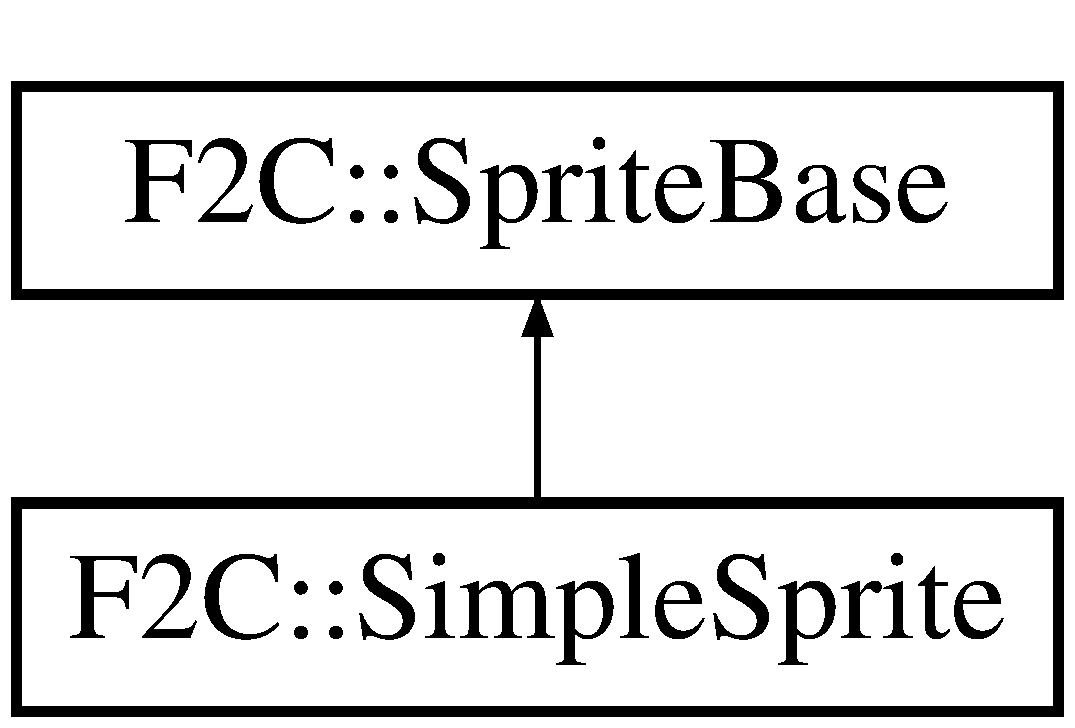
\includegraphics[height=2cm]{class_f2_c_1_1_simple_sprite}
\end{center}
\end{figure}
\subsection*{Public Member Functions}
\begin{DoxyCompactItemize}
\item 
\hypertarget{class_f2_c_1_1_simple_sprite_ae3616dd933524b2aa481d20e2f954e91}{
\hyperlink{class_f2_c_1_1_simple_sprite_ae3616dd933524b2aa481d20e2f954e91}{SimpleSprite} ()}
\label{class_f2_c_1_1_simple_sprite_ae3616dd933524b2aa481d20e2f954e91}

\begin{DoxyCompactList}\small\item\em Default constructor. \item\end{DoxyCompactList}\item 
\hyperlink{class_f2_c_1_1_simple_sprite_a47a25751dcc327438aebf044bafb566d}{SimpleSprite} (const \hyperlink{class_f2_c_1_1_bitmap}{Bitmap} $\ast$bitmap)
\begin{DoxyCompactList}\small\item\em Load the pixels from the bitmap into the texture. If NULL, is equivalent to the behavior as a disabled texturing. \item\end{DoxyCompactList}\item 
\hypertarget{class_f2_c_1_1_simple_sprite_a2449ff78a09f748094bc2a75df69eaba}{
\hyperlink{class_f2_c_1_1_simple_sprite_a2449ff78a09f748094bc2a75df69eaba}{SimpleSprite} (const \hyperlink{class_f2_c_1_1_simple_sprite}{SimpleSprite} \&copy)}
\label{class_f2_c_1_1_simple_sprite_a2449ff78a09f748094bc2a75df69eaba}

\begin{DoxyCompactList}\small\item\em Copy constructor. \item\end{DoxyCompactList}\item 
\hypertarget{class_f2_c_1_1_simple_sprite_aebf2619b56afa24816fdf95f236d5790}{
\hyperlink{class_f2_c_1_1_simple_sprite}{SimpleSprite} \& \hyperlink{class_f2_c_1_1_simple_sprite_aebf2619b56afa24816fdf95f236d5790}{operator=} (const \hyperlink{class_f2_c_1_1_simple_sprite}{SimpleSprite} \&copy)}
\label{class_f2_c_1_1_simple_sprite_aebf2619b56afa24816fdf95f236d5790}

\begin{DoxyCompactList}\small\item\em Assignment operator with deep copy. \item\end{DoxyCompactList}\item 
void \hyperlink{class_f2_c_1_1_simple_sprite_a1aa8944250c186b4a88c7bf7850fbb67}{copyProperties} (const \hyperlink{class_f2_c_1_1_simple_sprite}{SimpleSprite} \&copy)
\begin{DoxyCompactList}\small\item\em Copies all properties(x,y,z-\/Coord.,vColor,...), except the texture(\hyperlink{class_f2_c_1_1_bitmap}{Bitmap},bitmapWidth,Height,...). \item\end{DoxyCompactList}\item 
int \hyperlink{class_f2_c_1_1_simple_sprite_a94d58e6e46796a7352486817d51a1c3f}{render} () const 
\begin{DoxyCompactList}\small\item\em Render the bitmap on screen. \item\end{DoxyCompactList}\end{DoxyCompactItemize}
\subsection*{Public Attributes}
\begin{DoxyCompactItemize}
\item 
\hypertarget{class_f2_c_1_1_simple_sprite_a72871a4bdff954844ebe4243aa859e13}{
\hyperlink{namespace_f2_c_a711deb33697d145669b9c0c4fe87c7ca}{uint8} \hyperlink{class_f2_c_1_1_simple_sprite_a72871a4bdff954844ebe4243aa859e13}{grayscale}}
\label{class_f2_c_1_1_simple_sprite_a72871a4bdff954844ebe4243aa859e13}

\begin{DoxyCompactList}\small\item\em Grayscale value (or the tranzperenz the shader generated image). \item\end{DoxyCompactList}\end{DoxyCompactItemize}
\subsection*{Static Public Attributes}
\begin{DoxyCompactItemize}
\item 
\hypertarget{class_f2_c_1_1_simple_sprite_a99c2e7a0334bc761eb1e2017c3fdf347}{
static GLhandleARB \hyperlink{class_f2_c_1_1_simple_sprite_a99c2e7a0334bc761eb1e2017c3fdf347}{ShaderProgramObj}}
\label{class_f2_c_1_1_simple_sprite_a99c2e7a0334bc761eb1e2017c3fdf347}

\begin{DoxyCompactList}\small\item\em Handle by the ARB program object for the \hyperlink{class_f2_c_1_1_array_sprite}{ArraySprite}. (Default: NULL) \par
 The Tranzperenz(Alpha Color) of the generated shader image (with the ARB program object) can be determined by the grayscale. \item\end{DoxyCompactList}\item 
\hypertarget{class_f2_c_1_1_simple_sprite_ae4a2a18c63ffab85ef5da18dc0366edc}{
static \hyperlink{namespace_f2_c_1_1_tex_param_a64299c3972944468af4e8b0394c936c6}{TexParam::Tex\_\-Param} \hyperlink{class_f2_c_1_1_simple_sprite_ae4a2a18c63ffab85ef5da18dc0366edc}{filter}}
\label{class_f2_c_1_1_simple_sprite_ae4a2a18c63ffab85ef5da18dc0366edc}

\begin{DoxyCompactList}\small\item\em Set the texture filtering of the \hyperlink{class_f2_c_1_1_sprite}{Sprite}. (Default: Linear). \item\end{DoxyCompactList}\end{DoxyCompactItemize}


\subsection{Detailed Description}
Renders an image (\hyperlink{class_f2_c_1_1_bitmap}{Bitmap} class) on the screen. This class offers less than the normal \hyperlink{class_f2_c_1_1_sprite}{Sprite} class is but a little faster at rendering. Please note the following OpenGL capability are enabled when rendering and at the end disable: \par
 GL\_\-TEXTURE\_\-2D \par
 GL\_\-DEPTH\_\-TEST \par
 GL\_\-ALPHA\_\-TEST \par
 GL\_\-BLEND \par
 and use glShadeModel(GL\_\-SMOOTH) \par
 \par
 Dont forget to set the depth and alpha test function, e.g.: \par
 glAlphaFunc(GL\_\-GREATER, 0.0f) \par
 glDepthFunc(GL\_\-LEQUAL) \par
 \par
 Used OpenGL Buffers \par
 -\/GL\_\-COLOR\_\-BUFFER\_\-BIT \par
 -\/GL\_\-DEPTH\_\-BUFFER\_\-BIT \par
 

\subsection{Constructor \& Destructor Documentation}
\hypertarget{class_f2_c_1_1_simple_sprite_a47a25751dcc327438aebf044bafb566d}{
\index{F2C::SimpleSprite@{F2C::SimpleSprite}!SimpleSprite@{SimpleSprite}}
\index{SimpleSprite@{SimpleSprite}!F2C::SimpleSprite@{F2C::SimpleSprite}}
\subsubsection[{SimpleSprite}]{\setlength{\rightskip}{0pt plus 5cm}F2C::SimpleSprite::SimpleSprite (const {\bf Bitmap} $\ast$ {\em bitmap})}}
\label{class_f2_c_1_1_simple_sprite_a47a25751dcc327438aebf044bafb566d}


Load the pixels from the bitmap into the texture. If NULL, is equivalent to the behavior as a disabled texturing. 
\begin{DoxyParams}{Parameters}
\item[{\em bitmap}]Pointer of \hyperlink{class_f2_c_1_1_bitmap}{Bitmap} \end{DoxyParams}


\subsection{Member Function Documentation}
\hypertarget{class_f2_c_1_1_simple_sprite_a1aa8944250c186b4a88c7bf7850fbb67}{
\index{F2C::SimpleSprite@{F2C::SimpleSprite}!copyProperties@{copyProperties}}
\index{copyProperties@{copyProperties}!F2C::SimpleSprite@{F2C::SimpleSprite}}
\subsubsection[{copyProperties}]{\setlength{\rightskip}{0pt plus 5cm}void F2C::SimpleSprite::copyProperties (const {\bf SimpleSprite} \& {\em copy})}}
\label{class_f2_c_1_1_simple_sprite_a1aa8944250c186b4a88c7bf7850fbb67}


Copies all properties(x,y,z-\/Coord.,vColor,...), except the texture(\hyperlink{class_f2_c_1_1_bitmap}{Bitmap},bitmapWidth,Height,...). 
\begin{DoxyParams}{Parameters}
\item[{\em copy}]Source copy \end{DoxyParams}


Reimplemented from \hyperlink{class_f2_c_1_1_sprite_base_a8f7ea8a95a07688bfb2e6268a52b9215}{F2C::SpriteBase}.\hypertarget{class_f2_c_1_1_simple_sprite_a94d58e6e46796a7352486817d51a1c3f}{
\index{F2C::SimpleSprite@{F2C::SimpleSprite}!render@{render}}
\index{render@{render}!F2C::SimpleSprite@{F2C::SimpleSprite}}
\subsubsection[{render}]{\setlength{\rightskip}{0pt plus 5cm}int F2C::SimpleSprite::render () const\hspace{0.3cm}{\ttfamily  \mbox{[}virtual\mbox{]}}}}
\label{class_f2_c_1_1_simple_sprite_a94d58e6e46796a7352486817d51a1c3f}


Render the bitmap on screen. \begin{DoxyReturn}{Returns}
-\/1, show is false. 

-\/2, The width or height of the bitmap or the src\_\-rect are 0. 

-\/3, The sprite is outside the display (glViewport). 

-\/4, The alpha color of all 4 Vertices are less than 1. 

-\/5, zoom\_\-x or zoom\_\-y is exactly 0. 

1, \hyperlink{class_f2_c_1_1_sprite}{Sprite} has been successfully rendered. 
\end{DoxyReturn}


Implements \hyperlink{class_f2_c_1_1_sprite_base_af9dfc70083ca5a774d3874b61a6f9abc}{F2C::SpriteBase}.
\hypertarget{class_f2_c_1_1_sprite}{
\section{F2C::Sprite Class Reference}
\label{class_f2_c_1_1_sprite}\index{F2C::Sprite@{F2C::Sprite}}
}


Renders an image (\hyperlink{class_f2_c_1_1_bitmap}{Bitmap} class) on the screen.  


Inheritance diagram for F2C::Sprite:\begin{figure}[H]
\begin{center}
\leavevmode
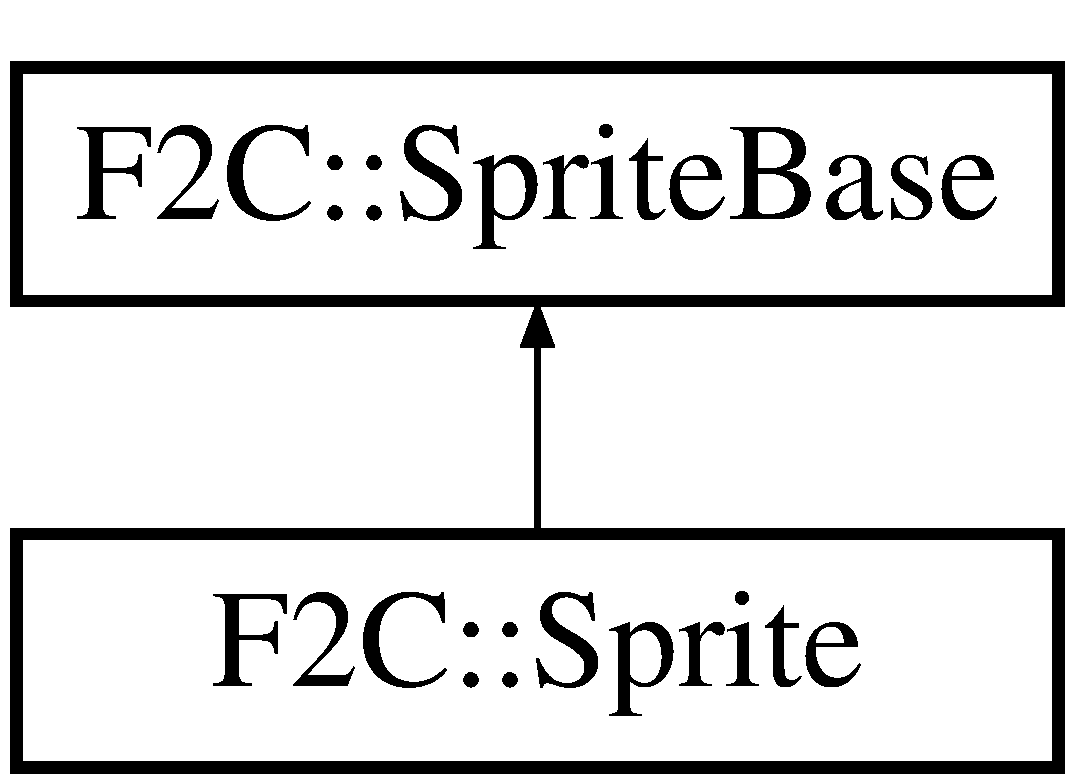
\includegraphics[height=2.000000cm]{class_f2_c_1_1_sprite}
\end{center}
\end{figure}
\subsection*{Public Member Functions}
\begin{DoxyCompactItemize}
\item 
\hypertarget{class_f2_c_1_1_sprite_adfbb0aa21734d8e4e24b50dffe00ada4}{
\hyperlink{class_f2_c_1_1_sprite_adfbb0aa21734d8e4e24b50dffe00ada4}{Sprite} ()}
\label{class_f2_c_1_1_sprite_adfbb0aa21734d8e4e24b50dffe00ada4}

\begin{DoxyCompactList}\small\item\em Default constructor. \item\end{DoxyCompactList}\item 
\hyperlink{class_f2_c_1_1_sprite_a858b8f2c06e804c19f6c6a5cbe760c1b}{Sprite} (\hyperlink{class_f2_c_1_1_viewport}{Viewport} $\ast$\hyperlink{class_f2_c_1_1_sprite_a66cc8d6922dcbf4331b360800ba47177}{viewport})
\begin{DoxyCompactList}\small\item\em Set the pointer of the viewport and the clip\_\-rect. \item\end{DoxyCompactList}\item 
\hyperlink{class_f2_c_1_1_sprite_a18cd93c504d29dfc9df20dcde1968c45}{Sprite} (const \hyperlink{class_f2_c_1_1_bitmap}{Bitmap} $\ast$bitmap)
\begin{DoxyCompactList}\small\item\em Load the pixels from the bitmap into the texture. If NULL, is equivalent to the behavior as a disabled texturing. \item\end{DoxyCompactList}\item 
\hypertarget{class_f2_c_1_1_sprite_a7efb0dbc78a120afa45db3b2e4c69e58}{
\hyperlink{class_f2_c_1_1_sprite_a7efb0dbc78a120afa45db3b2e4c69e58}{Sprite} (const \hyperlink{class_f2_c_1_1_sprite}{Sprite} \&copy)}
\label{class_f2_c_1_1_sprite_a7efb0dbc78a120afa45db3b2e4c69e58}

\begin{DoxyCompactList}\small\item\em Copy constructor. \item\end{DoxyCompactList}\item 
\hypertarget{class_f2_c_1_1_sprite_a8bcf707d839630b917e9479bc2380c16}{
\hyperlink{class_f2_c_1_1_sprite}{Sprite} \& \hyperlink{class_f2_c_1_1_sprite_a8bcf707d839630b917e9479bc2380c16}{operator=} (const \hyperlink{class_f2_c_1_1_sprite}{Sprite} \&copy)}
\label{class_f2_c_1_1_sprite_a8bcf707d839630b917e9479bc2380c16}

\begin{DoxyCompactList}\small\item\em Assignment operator with deep copy. \item\end{DoxyCompactList}\item 
void \hyperlink{class_f2_c_1_1_sprite_a33d27869102b12705666a1712d9f645d}{copyProperties} (const \hyperlink{class_f2_c_1_1_sprite}{Sprite} \&copy)
\begin{DoxyCompactList}\small\item\em Copies all properties(x,y,z-\/Coord.,vColor,...), except the texture(\hyperlink{class_f2_c_1_1_bitmap}{Bitmap},bitmapWidth,Height,...). \item\end{DoxyCompactList}\item 
int \hyperlink{class_f2_c_1_1_sprite_a53505010baf74857c67c82150802b297}{render} () const 
\begin{DoxyCompactList}\small\item\em Render the bitmap on screen. \item\end{DoxyCompactList}\item 
void \hyperlink{class_f2_c_1_1_sprite_a8bc4649a6100c8b26c67c94e79497289}{setViewport} (\hyperlink{class_f2_c_1_1_viewport}{Viewport} $\ast$\hyperlink{class_f2_c_1_1_sprite_a66cc8d6922dcbf4331b360800ba47177}{viewport})
\begin{DoxyCompactList}\small\item\em setMethode: Set the pointer of the viewport and the clip\_\-rect. \item\end{DoxyCompactList}\end{DoxyCompactItemize}
\subsection*{Static Public Member Functions}
\begin{DoxyCompactItemize}
\item 
static void \hyperlink{class_f2_c_1_1_sprite_aa237fe3dca3002ea876865cfde83bfa3}{enableGLDrawArray} (bool enable)
\begin{DoxyCompactList}\small\item\em if enable then use glDrawArrays,glEnableClientState,... , if disable then use glBegin(),glVertex(),...,glEnd(). \par
 Is automatically enable when VBO is supported. \item\end{DoxyCompactList}\item 
\hypertarget{class_f2_c_1_1_sprite_ae5bff6a95dbabc64de9143e59c708ab4}{
static bool \hyperlink{class_f2_c_1_1_sprite_ae5bff6a95dbabc64de9143e59c708ab4}{isEnableGLDrawArray} ()}
\label{class_f2_c_1_1_sprite_ae5bff6a95dbabc64de9143e59c708ab4}

\begin{DoxyCompactList}\small\item\em getMethode: Is glDrawArrays,glEnableClientState,... used when rendering. \item\end{DoxyCompactList}\end{DoxyCompactItemize}
\subsection*{Public Attributes}
\begin{DoxyCompactItemize}
\item 
\hypertarget{class_f2_c_1_1_sprite_aa03b4a6e204fb24f935d42bf0d40b1bd}{
\hyperlink{class_f2_c_1_1_rect}{Rect} $\ast$ \hyperlink{class_f2_c_1_1_sprite_aa03b4a6e204fb24f935d42bf0d40b1bd}{clip\_\-rect}}
\label{class_f2_c_1_1_sprite_aa03b4a6e204fb24f935d42bf0d40b1bd}

\begin{DoxyCompactList}\small\item\em Clipping \hyperlink{class_f2_c_1_1_rect}{Rect}, Cutting the sprites on the screen the desired section or window. \item\end{DoxyCompactList}\item 
\hypertarget{class_f2_c_1_1_sprite_a66cc8d6922dcbf4331b360800ba47177}{
\hyperlink{class_f2_c_1_1_viewport}{Viewport} $\ast$ \hyperlink{class_f2_c_1_1_sprite_a66cc8d6922dcbf4331b360800ba47177}{viewport}}
\label{class_f2_c_1_1_sprite_a66cc8d6922dcbf4331b360800ba47177}

\begin{DoxyCompactList}\small\item\em Additional Z-\/coordinate and \hyperlink{class_f2_c_1_1_color_tone}{ColorTone}. \item\end{DoxyCompactList}\item 
\hypertarget{class_f2_c_1_1_sprite_aa1b34c2ac3927922793a729b63046b06}{
\hyperlink{class_f2_c_1_1_color_tone}{ColorTone} \hyperlink{class_f2_c_1_1_sprite_aa1b34c2ac3927922793a729b63046b06}{tone}}
\label{class_f2_c_1_1_sprite_aa1b34c2ac3927922793a729b63046b06}

\begin{DoxyCompactList}\small\item\em \hyperlink{class_f2_c_1_1_color}{Color} tone. \item\end{DoxyCompactList}\end{DoxyCompactItemize}
\subsection*{Static Public Attributes}
\begin{DoxyCompactItemize}
\item 
\hypertarget{class_f2_c_1_1_sprite_adb167a247bc75717c96e587e3b2c8993}{
static GLhandleARB \hyperlink{class_f2_c_1_1_sprite_adb167a247bc75717c96e587e3b2c8993}{ShaderProgramObj}}
\label{class_f2_c_1_1_sprite_adb167a247bc75717c96e587e3b2c8993}

\begin{DoxyCompactList}\small\item\em Handle by the ARB program object for the \hyperlink{class_f2_c_1_1_array_sprite}{ArraySprite}. (Default: NULL) \par
 The Tranzperenz(Alpha Color) of the generated shader image (with the ARB program object) can be determined by the grayscale. \item\end{DoxyCompactList}\item 
\hypertarget{class_f2_c_1_1_sprite_afdc906dcee337188d0a8bc5b054c5e09}{
static \hyperlink{namespace_f2_c_1_1_tex_param_a64299c3972944468af4e8b0394c936c6}{TexParam::Tex\_\-Param} \hyperlink{class_f2_c_1_1_sprite_afdc906dcee337188d0a8bc5b054c5e09}{filter}}
\label{class_f2_c_1_1_sprite_afdc906dcee337188d0a8bc5b054c5e09}

\begin{DoxyCompactList}\small\item\em Set the texture filtering of the \hyperlink{class_f2_c_1_1_sprite}{Sprite}. (Default: Linear). \item\end{DoxyCompactList}\end{DoxyCompactItemize}
\subsection*{Friends}
\begin{DoxyCompactItemize}
\item 
std::ostream \& \hyperlink{class_f2_c_1_1_sprite_a0b5b0f19eaf4188e211f3bc41b82673c}{operator$<$$<$} (std::ostream \&out, const \hyperlink{class_f2_c_1_1_sprite}{Sprite} \&obj)
\begin{DoxyCompactList}\small\item\em Write the Object into output stream. (dont write pointer (\hyperlink{class_f2_c_1_1_viewport}{Viewport},clip\_\-rect)). \item\end{DoxyCompactList}\item 
std::istream \& \hyperlink{class_f2_c_1_1_sprite_a591a1f6d79479eca4af4b3d55e85a562}{operator$>$$>$} (std::istream \&in, \hyperlink{class_f2_c_1_1_sprite}{Sprite} \&obj)
\begin{DoxyCompactList}\small\item\em Read the Object from input stream. (dont read pointer (\hyperlink{class_f2_c_1_1_viewport}{Viewport},clip\_\-rect)). \item\end{DoxyCompactList}\end{DoxyCompactItemize}


\subsection{Detailed Description}
Renders an image (\hyperlink{class_f2_c_1_1_bitmap}{Bitmap} class) on the screen. Please note the following OpenGL capability are enabled when rendering and at the end disable: \par
 GL\_\-SCISSOR\_\-TEST (if necessary) \par
 GL\_\-STENCIL\_\-TEST \par
 GL\_\-TEXTURE\_\-2D \par
 GL\_\-DEPTH\_\-TEST \par
 GL\_\-ALPHA\_\-TEST \par
 GL\_\-BLEND \par
 and use glShadeModel(GL\_\-SMOOTH) \par
 \par
 Dont forget to set the depth and alpha test function, e.g.: \par
 glAlphaFunc(GL\_\-GREATER, 0.0f) \par
 glDepthFunc(GL\_\-LEQUAL) \par
 \par
 Used OpenGL Buffers \par
 -\/GL\_\-COLOR\_\-BUFFER\_\-BIT \par
 -\/GL\_\-DEPTH\_\-BUFFER\_\-BIT \par
 -\/GL\_\-STENCIL\_\-BUFFER\_\-BIT \par
 

\subsection{Constructor \& Destructor Documentation}
\hypertarget{class_f2_c_1_1_sprite_a858b8f2c06e804c19f6c6a5cbe760c1b}{
\index{F2C::Sprite@{F2C::Sprite}!Sprite@{Sprite}}
\index{Sprite@{Sprite}!F2C::Sprite@{F2C::Sprite}}
\subsubsection[{Sprite}]{\setlength{\rightskip}{0pt plus 5cm}F2C::Sprite::Sprite (
\begin{DoxyParamCaption}
\item[{{\bf Viewport} $\ast$}]{ viewport}
\end{DoxyParamCaption}
)}}
\label{class_f2_c_1_1_sprite_a858b8f2c06e804c19f6c6a5cbe760c1b}


Set the pointer of the viewport and the clip\_\-rect. 


\begin{DoxyParams}{Parameters}
\item[{\em viewport}]Pointer of \hyperlink{class_f2_c_1_1_viewport}{Viewport} \end{DoxyParams}
\hypertarget{class_f2_c_1_1_sprite_a18cd93c504d29dfc9df20dcde1968c45}{
\index{F2C::Sprite@{F2C::Sprite}!Sprite@{Sprite}}
\index{Sprite@{Sprite}!F2C::Sprite@{F2C::Sprite}}
\subsubsection[{Sprite}]{\setlength{\rightskip}{0pt plus 5cm}F2C::Sprite::Sprite (
\begin{DoxyParamCaption}
\item[{const {\bf Bitmap} $\ast$}]{ bitmap}
\end{DoxyParamCaption}
)}}
\label{class_f2_c_1_1_sprite_a18cd93c504d29dfc9df20dcde1968c45}


Load the pixels from the bitmap into the texture. If NULL, is equivalent to the behavior as a disabled texturing. 


\begin{DoxyParams}{Parameters}
\item[{\em bitmap}]Pointer of \hyperlink{class_f2_c_1_1_bitmap}{Bitmap} \end{DoxyParams}


\subsection{Member Function Documentation}
\hypertarget{class_f2_c_1_1_sprite_a33d27869102b12705666a1712d9f645d}{
\index{F2C::Sprite@{F2C::Sprite}!copyProperties@{copyProperties}}
\index{copyProperties@{copyProperties}!F2C::Sprite@{F2C::Sprite}}
\subsubsection[{copyProperties}]{\setlength{\rightskip}{0pt plus 5cm}void F2C::Sprite::copyProperties (
\begin{DoxyParamCaption}
\item[{const {\bf Sprite} \&}]{ copy}
\end{DoxyParamCaption}
)}}
\label{class_f2_c_1_1_sprite_a33d27869102b12705666a1712d9f645d}


Copies all properties(x,y,z-\/Coord.,vColor,...), except the texture(\hyperlink{class_f2_c_1_1_bitmap}{Bitmap},bitmapWidth,Height,...). 


\begin{DoxyParams}{Parameters}
\item[{\em copy}]Source copy \end{DoxyParams}
\hypertarget{class_f2_c_1_1_sprite_aa237fe3dca3002ea876865cfde83bfa3}{
\index{F2C::Sprite@{F2C::Sprite}!enableGLDrawArray@{enableGLDrawArray}}
\index{enableGLDrawArray@{enableGLDrawArray}!F2C::Sprite@{F2C::Sprite}}
\subsubsection[{enableGLDrawArray}]{\setlength{\rightskip}{0pt plus 5cm}static void F2C::Sprite::enableGLDrawArray (
\begin{DoxyParamCaption}
\item[{bool}]{ enable}
\end{DoxyParamCaption}
)\hspace{0.3cm}{\ttfamily  \mbox{[}static\mbox{]}}}}
\label{class_f2_c_1_1_sprite_aa237fe3dca3002ea876865cfde83bfa3}


if enable then use glDrawArrays,glEnableClientState,... , if disable then use glBegin(),glVertex(),...,glEnd(). \par
 Is automatically enable when VBO is supported. 


\begin{DoxyParams}{Parameters}
\item[{\em enable}]Enable/Disable \end{DoxyParams}
\hypertarget{class_f2_c_1_1_sprite_a53505010baf74857c67c82150802b297}{
\index{F2C::Sprite@{F2C::Sprite}!render@{render}}
\index{render@{render}!F2C::Sprite@{F2C::Sprite}}
\subsubsection[{render}]{\setlength{\rightskip}{0pt plus 5cm}int F2C::Sprite::render (
\begin{DoxyParamCaption}
{}
\end{DoxyParamCaption}
) const\hspace{0.3cm}{\ttfamily  \mbox{[}virtual\mbox{]}}}}
\label{class_f2_c_1_1_sprite_a53505010baf74857c67c82150802b297}


Render the bitmap on screen. 

\begin{DoxyReturn}{Returns}
-\/1, show is false (or from viewport). 

-\/2, The width or height of the bitmap or the src\_\-rect are 0. 

-\/3, The sprite is outside the display (glViewport). 

-\/4, The alpha color of all 4 Vertices are less than 1. 

-\/5, zoom\_\-x or zoom\_\-y is exactly 0. 

1, \hyperlink{class_f2_c_1_1_sprite}{Sprite} has been successfully rendered. 
\end{DoxyReturn}


Implements \hyperlink{class_f2_c_1_1_sprite_base_af9dfc70083ca5a774d3874b61a6f9abc}{F2C::SpriteBase}.

\hypertarget{class_f2_c_1_1_sprite_a8bc4649a6100c8b26c67c94e79497289}{
\index{F2C::Sprite@{F2C::Sprite}!setViewport@{setViewport}}
\index{setViewport@{setViewport}!F2C::Sprite@{F2C::Sprite}}
\subsubsection[{setViewport}]{\setlength{\rightskip}{0pt plus 5cm}void F2C::Sprite::setViewport (
\begin{DoxyParamCaption}
\item[{{\bf Viewport} $\ast$}]{ viewport}
\end{DoxyParamCaption}
)}}
\label{class_f2_c_1_1_sprite_a8bc4649a6100c8b26c67c94e79497289}


setMethode: Set the pointer of the viewport and the clip\_\-rect. 


\begin{DoxyParams}{Parameters}
\item[{\em viewport}]Pointer of \hyperlink{class_f2_c_1_1_viewport}{Viewport} \end{DoxyParams}


\subsection{Friends And Related Function Documentation}
\hypertarget{class_f2_c_1_1_sprite_a0b5b0f19eaf4188e211f3bc41b82673c}{
\index{F2C::Sprite@{F2C::Sprite}!operator$<$$<$@{operator$<$$<$}}
\index{operator$<$$<$@{operator$<$$<$}!F2C::Sprite@{F2C::Sprite}}
\subsubsection[{operator$<$$<$}]{\setlength{\rightskip}{0pt plus 5cm}std::ostream\& operator$<$$<$ (
\begin{DoxyParamCaption}
\item[{std::ostream \&}]{ out, }
\item[{const {\bf Sprite} \&}]{ obj}
\end{DoxyParamCaption}
)\hspace{0.3cm}{\ttfamily  \mbox{[}friend\mbox{]}}}}
\label{class_f2_c_1_1_sprite_a0b5b0f19eaf4188e211f3bc41b82673c}


Write the Object into output stream. (dont write pointer (\hyperlink{class_f2_c_1_1_viewport}{Viewport},clip\_\-rect)). 


\begin{DoxyParams}{Parameters}
\item[{\em out}]Output stream \item[{\em obj}]Object \end{DoxyParams}
\hypertarget{class_f2_c_1_1_sprite_a591a1f6d79479eca4af4b3d55e85a562}{
\index{F2C::Sprite@{F2C::Sprite}!operator$>$$>$@{operator$>$$>$}}
\index{operator$>$$>$@{operator$>$$>$}!F2C::Sprite@{F2C::Sprite}}
\subsubsection[{operator$>$$>$}]{\setlength{\rightskip}{0pt plus 5cm}std::istream\& operator$>$$>$ (
\begin{DoxyParamCaption}
\item[{std::istream \&}]{ in, }
\item[{{\bf Sprite} \&}]{ obj}
\end{DoxyParamCaption}
)\hspace{0.3cm}{\ttfamily  \mbox{[}friend\mbox{]}}}}
\label{class_f2_c_1_1_sprite_a591a1f6d79479eca4af4b3d55e85a562}


Read the Object from input stream. (dont read pointer (\hyperlink{class_f2_c_1_1_viewport}{Viewport},clip\_\-rect)). 


\begin{DoxyParams}{Parameters}
\item[{\em in}]\hyperlink{class_f2_c_1_1_input}{Input} stream \item[{\em obj}]Object \end{DoxyParams}

\hypertarget{class_f2_c_1_1_sprite_base}{
\section{F2C::SpriteBase Class Reference}
\label{class_f2_c_1_1_sprite_base}\index{F2C::SpriteBase@{F2C::SpriteBase}}
}


Basis Class of \hyperlink{class_f2_c_1_1_sprite}{Sprite}.  
Inheritance diagram for F2C::SpriteBase::\begin{figure}[H]
\begin{center}
\leavevmode
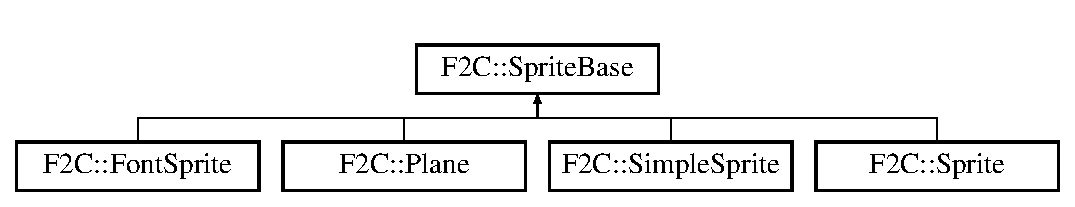
\includegraphics[height=2cm]{class_f2_c_1_1_sprite_base}
\end{center}
\end{figure}
\subsection*{Public Member Functions}
\begin{DoxyCompactItemize}
\item 
\hypertarget{class_f2_c_1_1_sprite_base_afbb00eac253f057d3ad63a2ac5cec749}{
\hyperlink{class_f2_c_1_1_sprite_base_afbb00eac253f057d3ad63a2ac5cec749}{SpriteBase} ()}
\label{class_f2_c_1_1_sprite_base_afbb00eac253f057d3ad63a2ac5cec749}

\begin{DoxyCompactList}\small\item\em Default constructor. \item\end{DoxyCompactList}\item 
\hypertarget{class_f2_c_1_1_sprite_base_a283941cc4bae11af8819212baedbc73d}{
virtual \hyperlink{class_f2_c_1_1_sprite_base_a283941cc4bae11af8819212baedbc73d}{$\sim$SpriteBase} ()}
\label{class_f2_c_1_1_sprite_base_a283941cc4bae11af8819212baedbc73d}

\begin{DoxyCompactList}\small\item\em Default destructor. \item\end{DoxyCompactList}\item 
\hyperlink{class_f2_c_1_1_sprite_base_aa00534841b3adc48e992e2282ec6963f}{SpriteBase} (const \hyperlink{class_f2_c_1_1_bitmap}{Bitmap} $\ast$bitmap)
\begin{DoxyCompactList}\small\item\em Load the pixels from the bitmap into the texture. If NULL, is equivalent to the behavior as a disabled texturing. \item\end{DoxyCompactList}\item 
\hypertarget{class_f2_c_1_1_sprite_base_a67e2731423751d23e05db92457ab7afe}{
\hyperlink{class_f2_c_1_1_sprite_base_a67e2731423751d23e05db92457ab7afe}{SpriteBase} (const \hyperlink{class_f2_c_1_1_sprite_base}{SpriteBase} \&copy)}
\label{class_f2_c_1_1_sprite_base_a67e2731423751d23e05db92457ab7afe}

\begin{DoxyCompactList}\small\item\em Copy constructor. \item\end{DoxyCompactList}\item 
\hypertarget{class_f2_c_1_1_sprite_base_af56c5ea473d444f4c8b65bd51d7fd724}{
\hyperlink{class_f2_c_1_1_sprite_base}{SpriteBase} \& \hyperlink{class_f2_c_1_1_sprite_base_af56c5ea473d444f4c8b65bd51d7fd724}{operator=} (const \hyperlink{class_f2_c_1_1_sprite_base}{SpriteBase} \&copy)}
\label{class_f2_c_1_1_sprite_base_af56c5ea473d444f4c8b65bd51d7fd724}

\begin{DoxyCompactList}\small\item\em Assignment operator with deep copy. \item\end{DoxyCompactList}\item 
void \hyperlink{class_f2_c_1_1_sprite_base_a8f7ea8a95a07688bfb2e6268a52b9215}{copyProperties} (const \hyperlink{class_f2_c_1_1_sprite_base}{SpriteBase} \&copy)
\begin{DoxyCompactList}\small\item\em Copies all properties(x,y,z-\/Coord.,vColor,...), except the texture(\hyperlink{class_f2_c_1_1_bitmap}{Bitmap},bitmapWidth,Height,...). \item\end{DoxyCompactList}\item 
\hypertarget{class_f2_c_1_1_sprite_base_af9dfc70083ca5a774d3874b61a6f9abc}{
virtual int \hyperlink{class_f2_c_1_1_sprite_base_af9dfc70083ca5a774d3874b61a6f9abc}{render} () const =0}
\label{class_f2_c_1_1_sprite_base_af9dfc70083ca5a774d3874b61a6f9abc}

\begin{DoxyCompactList}\small\item\em Render the bitmap on screen. \item\end{DoxyCompactList}\item 
void \hyperlink{class_f2_c_1_1_sprite_base_a4a931a54423a0aae08eacc30e96d485f}{setRed} (\hyperlink{namespace_f2_c_a711deb33697d145669b9c0c4fe87c7ca}{uint8} red)
\begin{DoxyCompactList}\small\item\em setMethode: Sets the color red of all 4 Vertices. \item\end{DoxyCompactList}\item 
void \hyperlink{class_f2_c_1_1_sprite_base_a22cb562ef6c8e857cf78cd3037dbfe48}{setGreen} (\hyperlink{namespace_f2_c_a711deb33697d145669b9c0c4fe87c7ca}{uint8} green)
\begin{DoxyCompactList}\small\item\em setMethode: Sets the color green of all 4 Vertices. \item\end{DoxyCompactList}\item 
void \hyperlink{class_f2_c_1_1_sprite_base_ae08702a286ecfde0cf4ef8aacc8c9656}{setBlue} (\hyperlink{namespace_f2_c_a711deb33697d145669b9c0c4fe87c7ca}{uint8} blue)
\begin{DoxyCompactList}\small\item\em setMethode: Sets the color blue of all 4 Vertices. \item\end{DoxyCompactList}\item 
void \hyperlink{class_f2_c_1_1_sprite_base_a476e1be82005a18cce5989a478d3f5a4}{setAlpha} (\hyperlink{namespace_f2_c_a711deb33697d145669b9c0c4fe87c7ca}{uint8} alpha)
\begin{DoxyCompactList}\small\item\em setMethode: Sets the color alpha of all 4 Vertices. \item\end{DoxyCompactList}\item 
void \hyperlink{class_f2_c_1_1_sprite_base_a8dea109774f2021855921952a55dad34}{setColor} (const \hyperlink{class_f2_c_1_1_color}{Color} \&color)
\begin{DoxyCompactList}\small\item\em setMethode: Sets all colors of the 4 Vertices. \item\end{DoxyCompactList}\item 
void \hyperlink{class_f2_c_1_1_sprite_base_a70ecaf3b26c6a7e1490d276895a82694}{setColor} (\hyperlink{namespace_f2_c_a711deb33697d145669b9c0c4fe87c7ca}{uint8} red, \hyperlink{namespace_f2_c_a711deb33697d145669b9c0c4fe87c7ca}{uint8} green, \hyperlink{namespace_f2_c_a711deb33697d145669b9c0c4fe87c7ca}{uint8} blue, \hyperlink{namespace_f2_c_a711deb33697d145669b9c0c4fe87c7ca}{uint8} alpha)
\begin{DoxyCompactList}\small\item\em setMethode: Sets all colors of the 4 Vertices. \item\end{DoxyCompactList}\item 
void \hyperlink{class_f2_c_1_1_sprite_base_ad28077e5723498e1257b461abd805395}{setColor} (\hyperlink{namespace_f2_c_a711deb33697d145669b9c0c4fe87c7ca}{uint8} red, \hyperlink{namespace_f2_c_a711deb33697d145669b9c0c4fe87c7ca}{uint8} green, \hyperlink{namespace_f2_c_a711deb33697d145669b9c0c4fe87c7ca}{uint8} blue)
\begin{DoxyCompactList}\small\item\em setMethode: Sets all colors of the 4 Vertices. \item\end{DoxyCompactList}\item 
\hypertarget{class_f2_c_1_1_sprite_base_ab7b28dcc3e7c3fc26a6ffe1ae9c35ff0}{
\hyperlink{namespace_f2_c_a58be2bac9eb3e3c99cb41b6008bf4fae}{uint} \hyperlink{class_f2_c_1_1_sprite_base_ab7b28dcc3e7c3fc26a6ffe1ae9c35ff0}{getTexture} () const }
\label{class_f2_c_1_1_sprite_base_ab7b28dcc3e7c3fc26a6ffe1ae9c35ff0}

\begin{DoxyCompactList}\small\item\em getMethode: OpenGL Texture Name(ID) \item\end{DoxyCompactList}\item 
\hypertarget{class_f2_c_1_1_sprite_base_a38e5444bfd4600d0d32b5bfe7c5661d4}{
\hyperlink{namespace_f2_c_a58be2bac9eb3e3c99cb41b6008bf4fae}{uint} \hyperlink{class_f2_c_1_1_sprite_base_a38e5444bfd4600d0d32b5bfe7c5661d4}{getTexWidth} () const }
\label{class_f2_c_1_1_sprite_base_a38e5444bfd4600d0d32b5bfe7c5661d4}

\begin{DoxyCompactList}\small\item\em getMethode: Width of the bitmap. \item\end{DoxyCompactList}\item 
\hypertarget{class_f2_c_1_1_sprite_base_a12c777b014bd94631e0d232e97b069c6}{
\hyperlink{namespace_f2_c_a58be2bac9eb3e3c99cb41b6008bf4fae}{uint} \hyperlink{class_f2_c_1_1_sprite_base_a12c777b014bd94631e0d232e97b069c6}{getTexHeight} () const }
\label{class_f2_c_1_1_sprite_base_a12c777b014bd94631e0d232e97b069c6}

\begin{DoxyCompactList}\small\item\em getMethode: Height of the bitmap. \item\end{DoxyCompactList}\item 
\hypertarget{class_f2_c_1_1_sprite_base_a1c2bcccea45cbe282628b7c7e43cd93c}{
\hyperlink{namespace_f2_c_a58be2bac9eb3e3c99cb41b6008bf4fae}{uint} \hyperlink{class_f2_c_1_1_sprite_base_a1c2bcccea45cbe282628b7c7e43cd93c}{getTexBits} () const }
\label{class_f2_c_1_1_sprite_base_a1c2bcccea45cbe282628b7c7e43cd93c}

\begin{DoxyCompactList}\small\item\em getMethode: \hyperlink{class_f2_c_1_1_color}{Color} depth (in bits) of the texture. \item\end{DoxyCompactList}\item 
\hypertarget{class_f2_c_1_1_sprite_base_ab5746d99d97e67289b493a6c022fdb58}{
Image::DataFormat \hyperlink{class_f2_c_1_1_sprite_base_ab5746d99d97e67289b493a6c022fdb58}{getTexDataFormat} () const }
\label{class_f2_c_1_1_sprite_base_ab5746d99d97e67289b493a6c022fdb58}

\begin{DoxyCompactList}\small\item\em getMethode: Pixel format of the texture. \item\end{DoxyCompactList}\item 
void \hyperlink{class_f2_c_1_1_sprite_base_a94df734d094880352b1dc517a9332faa}{setBitmap} (const \hyperlink{class_f2_c_1_1_bitmap}{Bitmap} $\ast$bitmap)
\begin{DoxyCompactList}\small\item\em Load the pixels from the bitmap into the texture. If NULL, is equivalent to the behavior as a disabled texturing. \item\end{DoxyCompactList}\end{DoxyCompactItemize}
\subsection*{Public Attributes}
\begin{DoxyCompactItemize}
\item 
\hypertarget{class_f2_c_1_1_sprite_base_a23497fb7cb08ffa9ac5c34ec7cf88ffd}{
\hyperlink{class_f2_c_1_1_rect}{Rect} \hyperlink{class_f2_c_1_1_sprite_base_a23497fb7cb08ffa9ac5c34ec7cf88ffd}{src\_\-rect}}
\label{class_f2_c_1_1_sprite_base_a23497fb7cb08ffa9ac5c34ec7cf88ffd}

\begin{DoxyCompactList}\small\item\em Show rect of \hyperlink{class_f2_c_1_1_sprite}{Sprite}. \item\end{DoxyCompactList}\item 
\hypertarget{class_f2_c_1_1_sprite_base_a41d8b0b48cdd4a066cf6af3f806ce900}{
bool \hyperlink{class_f2_c_1_1_sprite_base_a41d8b0b48cdd4a066cf6af3f806ce900}{show}}
\label{class_f2_c_1_1_sprite_base_a41d8b0b48cdd4a066cf6af3f806ce900}

\begin{DoxyCompactList}\small\item\em Show \hyperlink{class_f2_c_1_1_sprite}{Sprite} On/Off. \item\end{DoxyCompactList}\item 
\hypertarget{class_f2_c_1_1_sprite_base_a552f88034a04e6ac41f22519ac53076c}{
int \hyperlink{class_f2_c_1_1_sprite_base_a552f88034a04e6ac41f22519ac53076c}{x}}
\label{class_f2_c_1_1_sprite_base_a552f88034a04e6ac41f22519ac53076c}

\begin{DoxyCompactList}\small\item\em X-\/coordinate. \item\end{DoxyCompactList}\item 
\hypertarget{class_f2_c_1_1_sprite_base_a33a3d48628d9a3130c603eaf902f209f}{
int \hyperlink{class_f2_c_1_1_sprite_base_a33a3d48628d9a3130c603eaf902f209f}{y}}
\label{class_f2_c_1_1_sprite_base_a33a3d48628d9a3130c603eaf902f209f}

\begin{DoxyCompactList}\small\item\em Y-\/coordinate. \item\end{DoxyCompactList}\item 
\hypertarget{class_f2_c_1_1_sprite_base_a9895daf6ea9ca00da376e8fed3f35f74}{
int \hyperlink{class_f2_c_1_1_sprite_base_a9895daf6ea9ca00da376e8fed3f35f74}{z}}
\label{class_f2_c_1_1_sprite_base_a9895daf6ea9ca00da376e8fed3f35f74}

\begin{DoxyCompactList}\small\item\em Z-\/coordinate. \item\end{DoxyCompactList}\item 
\hypertarget{class_f2_c_1_1_sprite_base_a9235af48d901047bec58ff47967a0448}{
double \hyperlink{class_f2_c_1_1_sprite_base_a9235af48d901047bec58ff47967a0448}{zoom\_\-x}}
\label{class_f2_c_1_1_sprite_base_a9235af48d901047bec58ff47967a0448}

\begin{DoxyCompactList}\small\item\em Zoom factor of the X-\/axis. \item\end{DoxyCompactList}\item 
\hypertarget{class_f2_c_1_1_sprite_base_a477efe5d34ffd44a7efa53886d4e6c5b}{
double \hyperlink{class_f2_c_1_1_sprite_base_a477efe5d34ffd44a7efa53886d4e6c5b}{zoom\_\-y}}
\label{class_f2_c_1_1_sprite_base_a477efe5d34ffd44a7efa53886d4e6c5b}

\begin{DoxyCompactList}\small\item\em Zoom factor of the Y-\/axis. \item\end{DoxyCompactList}\item 
\hypertarget{class_f2_c_1_1_sprite_base_abf960116205e3bfdd3931f1425573983}{
int \hyperlink{class_f2_c_1_1_sprite_base_abf960116205e3bfdd3931f1425573983}{angle\_\-x}}
\label{class_f2_c_1_1_sprite_base_abf960116205e3bfdd3931f1425573983}

\begin{DoxyCompactList}\small\item\em Rotation angle (in degrees) of the X-\/axis. \item\end{DoxyCompactList}\item 
\hypertarget{class_f2_c_1_1_sprite_base_a457087831441f94ca1bde73e7b1f9807}{
int \hyperlink{class_f2_c_1_1_sprite_base_a457087831441f94ca1bde73e7b1f9807}{angle\_\-y}}
\label{class_f2_c_1_1_sprite_base_a457087831441f94ca1bde73e7b1f9807}

\begin{DoxyCompactList}\small\item\em Rotation angle (in degrees) of the Y-\/axis. \item\end{DoxyCompactList}\item 
\hypertarget{class_f2_c_1_1_sprite_base_a5b407a83fd63a06e4fd6ab27f2086bd0}{
int \hyperlink{class_f2_c_1_1_sprite_base_a5b407a83fd63a06e4fd6ab27f2086bd0}{angle\_\-z}}
\label{class_f2_c_1_1_sprite_base_a5b407a83fd63a06e4fd6ab27f2086bd0}

\begin{DoxyCompactList}\small\item\em Rotation angle (in degrees) of the Z-\/axis. \item\end{DoxyCompactList}\item 
\hypertarget{class_f2_c_1_1_sprite_base_a24e4acd632808884f0c5e573afbdbb4a}{
\hyperlink{namespace_f2_c_1_1_blend_type_a582fe2d83fb813041785794568e5a414}{BlendType::Blend\_\-Type} \hyperlink{class_f2_c_1_1_sprite_base_a24e4acd632808884f0c5e573afbdbb4a}{blend\_\-type}}
\label{class_f2_c_1_1_sprite_base_a24e4acd632808884f0c5e573afbdbb4a}

\begin{DoxyCompactList}\small\item\em Blending type. \item\end{DoxyCompactList}\item 
\hyperlink{class_f2_c_1_1_color}{Color} \hyperlink{class_f2_c_1_1_sprite_base_ae05d180666e3750a5d5f909f04e686c4}{vColor} \mbox{[}4\mbox{]}
\begin{DoxyCompactList}\small\item\em Colors of the 4 Vertices. \item\end{DoxyCompactList}\end{DoxyCompactItemize}
\subsection*{Protected Attributes}
\begin{DoxyCompactItemize}
\item 
\hypertarget{class_f2_c_1_1_sprite_base_aa85f4d27f67d076a0fcbd90ff2786be4}{
GLuint \hyperlink{class_f2_c_1_1_sprite_base_aa85f4d27f67d076a0fcbd90ff2786be4}{texture}}
\label{class_f2_c_1_1_sprite_base_aa85f4d27f67d076a0fcbd90ff2786be4}

\begin{DoxyCompactList}\small\item\em OpenGL Texture Name(ID). \item\end{DoxyCompactList}\item 
\hypertarget{class_f2_c_1_1_sprite_base_a3beb2a38c8b3bb83de7c6c9815b3380e}{
\hyperlink{namespace_f2_c_a58be2bac9eb3e3c99cb41b6008bf4fae}{uint} \hyperlink{class_f2_c_1_1_sprite_base_a3beb2a38c8b3bb83de7c6c9815b3380e}{bitmapWidth}}
\label{class_f2_c_1_1_sprite_base_a3beb2a38c8b3bb83de7c6c9815b3380e}

\begin{DoxyCompactList}\small\item\em \hyperlink{class_f2_c_1_1_bitmap}{Bitmap} width. \item\end{DoxyCompactList}\item 
\hypertarget{class_f2_c_1_1_sprite_base_a6b8f515cbb9260887b6be67b9787f9d9}{
\hyperlink{namespace_f2_c_a58be2bac9eb3e3c99cb41b6008bf4fae}{uint} \hyperlink{class_f2_c_1_1_sprite_base_a6b8f515cbb9260887b6be67b9787f9d9}{bitmapHeight}}
\label{class_f2_c_1_1_sprite_base_a6b8f515cbb9260887b6be67b9787f9d9}

\begin{DoxyCompactList}\small\item\em \hyperlink{class_f2_c_1_1_bitmap}{Bitmap} height. \item\end{DoxyCompactList}\item 
\hypertarget{class_f2_c_1_1_sprite_base_ac14c1c3f97eafdcc312c92f7ceb1a144}{
\hyperlink{namespace_f2_c_a58be2bac9eb3e3c99cb41b6008bf4fae}{uint} \hyperlink{class_f2_c_1_1_sprite_base_ac14c1c3f97eafdcc312c92f7ceb1a144}{pixelsWidth}}
\label{class_f2_c_1_1_sprite_base_ac14c1c3f97eafdcc312c92f7ceb1a144}

\begin{DoxyCompactList}\small\item\em Width (or height) of the pixel array. \item\end{DoxyCompactList}\item 
\hypertarget{class_f2_c_1_1_sprite_base_a8e67797533a19e21ba9195b9679566b8}{
\hyperlink{namespace_f2_c_a74fad364688add30796d711e5635ac77}{ubyte} $\ast$ \hyperlink{class_f2_c_1_1_sprite_base_a8e67797533a19e21ba9195b9679566b8}{pixels}}
\label{class_f2_c_1_1_sprite_base_a8e67797533a19e21ba9195b9679566b8}

\begin{DoxyCompactList}\small\item\em Copy of pixels. \item\end{DoxyCompactList}\item 
\hypertarget{class_f2_c_1_1_sprite_base_a3f77c0311c6528deddc24e09bd132011}{
Image::DataFormat \hyperlink{class_f2_c_1_1_sprite_base_a3f77c0311c6528deddc24e09bd132011}{bitmapFormat}}
\label{class_f2_c_1_1_sprite_base_a3f77c0311c6528deddc24e09bd132011}

\begin{DoxyCompactList}\small\item\em Pixel data format. \item\end{DoxyCompactList}\item 
\hypertarget{class_f2_c_1_1_sprite_base_aace539201a27ea859def56d690cc47f9}{
\hyperlink{namespace_f2_c_a58be2bac9eb3e3c99cb41b6008bf4fae}{uint} \hyperlink{class_f2_c_1_1_sprite_base_aace539201a27ea859def56d690cc47f9}{bitmapBits}}
\label{class_f2_c_1_1_sprite_base_aace539201a27ea859def56d690cc47f9}

\begin{DoxyCompactList}\small\item\em Bits per pixel (color depth (in bits)). \item\end{DoxyCompactList}\end{DoxyCompactItemize}


\subsection{Detailed Description}
Basis Class of \hyperlink{class_f2_c_1_1_sprite}{Sprite}. 

\subsection{Constructor \& Destructor Documentation}
\hypertarget{class_f2_c_1_1_sprite_base_aa00534841b3adc48e992e2282ec6963f}{
\index{F2C::SpriteBase@{F2C::SpriteBase}!SpriteBase@{SpriteBase}}
\index{SpriteBase@{SpriteBase}!F2C::SpriteBase@{F2C::SpriteBase}}
\subsubsection[{SpriteBase}]{\setlength{\rightskip}{0pt plus 5cm}F2C::SpriteBase::SpriteBase (const {\bf Bitmap} $\ast$ {\em bitmap})}}
\label{class_f2_c_1_1_sprite_base_aa00534841b3adc48e992e2282ec6963f}


Load the pixels from the bitmap into the texture. If NULL, is equivalent to the behavior as a disabled texturing. 
\begin{DoxyParams}{Parameters}
\item[{\em bitmap}]Pointer of \hyperlink{class_f2_c_1_1_bitmap}{Bitmap} \end{DoxyParams}


\subsection{Member Function Documentation}
\hypertarget{class_f2_c_1_1_sprite_base_a8f7ea8a95a07688bfb2e6268a52b9215}{
\index{F2C::SpriteBase@{F2C::SpriteBase}!copyProperties@{copyProperties}}
\index{copyProperties@{copyProperties}!F2C::SpriteBase@{F2C::SpriteBase}}
\subsubsection[{copyProperties}]{\setlength{\rightskip}{0pt plus 5cm}void F2C::SpriteBase::copyProperties (const {\bf SpriteBase} \& {\em copy})}}
\label{class_f2_c_1_1_sprite_base_a8f7ea8a95a07688bfb2e6268a52b9215}


Copies all properties(x,y,z-\/Coord.,vColor,...), except the texture(\hyperlink{class_f2_c_1_1_bitmap}{Bitmap},bitmapWidth,Height,...). 
\begin{DoxyParams}{Parameters}
\item[{\em copy}]Source copy \end{DoxyParams}


Reimplemented in \hyperlink{class_f2_c_1_1_font_sprite_a36a224f59737fb06c4d79ee48b7e4068}{F2C::FontSprite}, \hyperlink{class_f2_c_1_1_plane_ac3ee4529b515cc641b6e9b27d76fc2ef}{F2C::Plane}, \hyperlink{class_f2_c_1_1_simple_sprite_a1aa8944250c186b4a88c7bf7850fbb67}{F2C::SimpleSprite}, and \hyperlink{class_f2_c_1_1_sprite_a33d27869102b12705666a1712d9f645d}{F2C::Sprite}.\hypertarget{class_f2_c_1_1_sprite_base_a476e1be82005a18cce5989a478d3f5a4}{
\index{F2C::SpriteBase@{F2C::SpriteBase}!setAlpha@{setAlpha}}
\index{setAlpha@{setAlpha}!F2C::SpriteBase@{F2C::SpriteBase}}
\subsubsection[{setAlpha}]{\setlength{\rightskip}{0pt plus 5cm}void F2C::SpriteBase::setAlpha ({\bf uint8} {\em alpha})}}
\label{class_f2_c_1_1_sprite_base_a476e1be82005a18cce5989a478d3f5a4}


setMethode: Sets the color alpha of all 4 Vertices. 
\begin{DoxyParams}{Parameters}
\item[{\em alpha}]Alpha \end{DoxyParams}
\hypertarget{class_f2_c_1_1_sprite_base_a94df734d094880352b1dc517a9332faa}{
\index{F2C::SpriteBase@{F2C::SpriteBase}!setBitmap@{setBitmap}}
\index{setBitmap@{setBitmap}!F2C::SpriteBase@{F2C::SpriteBase}}
\subsubsection[{setBitmap}]{\setlength{\rightskip}{0pt plus 5cm}void F2C::SpriteBase::setBitmap (const {\bf Bitmap} $\ast$ {\em bitmap})}}
\label{class_f2_c_1_1_sprite_base_a94df734d094880352b1dc517a9332faa}


Load the pixels from the bitmap into the texture. If NULL, is equivalent to the behavior as a disabled texturing. 
\begin{DoxyParams}{Parameters}
\item[{\em bitmap}]Pointer of \hyperlink{class_f2_c_1_1_bitmap}{Bitmap} \end{DoxyParams}
\hypertarget{class_f2_c_1_1_sprite_base_ae08702a286ecfde0cf4ef8aacc8c9656}{
\index{F2C::SpriteBase@{F2C::SpriteBase}!setBlue@{setBlue}}
\index{setBlue@{setBlue}!F2C::SpriteBase@{F2C::SpriteBase}}
\subsubsection[{setBlue}]{\setlength{\rightskip}{0pt plus 5cm}void F2C::SpriteBase::setBlue ({\bf uint8} {\em blue})}}
\label{class_f2_c_1_1_sprite_base_ae08702a286ecfde0cf4ef8aacc8c9656}


setMethode: Sets the color blue of all 4 Vertices. 
\begin{DoxyParams}{Parameters}
\item[{\em blue}]Blue \end{DoxyParams}
\hypertarget{class_f2_c_1_1_sprite_base_ad28077e5723498e1257b461abd805395}{
\index{F2C::SpriteBase@{F2C::SpriteBase}!setColor@{setColor}}
\index{setColor@{setColor}!F2C::SpriteBase@{F2C::SpriteBase}}
\subsubsection[{setColor}]{\setlength{\rightskip}{0pt plus 5cm}void F2C::SpriteBase::setColor ({\bf uint8} {\em red}, \/  {\bf uint8} {\em green}, \/  {\bf uint8} {\em blue})}}
\label{class_f2_c_1_1_sprite_base_ad28077e5723498e1257b461abd805395}


setMethode: Sets all colors of the 4 Vertices. 
\begin{DoxyParams}{Parameters}
\item[{\em red}]Red \item[{\em green}]Green \item[{\em blue}]Blue \end{DoxyParams}
\hypertarget{class_f2_c_1_1_sprite_base_a70ecaf3b26c6a7e1490d276895a82694}{
\index{F2C::SpriteBase@{F2C::SpriteBase}!setColor@{setColor}}
\index{setColor@{setColor}!F2C::SpriteBase@{F2C::SpriteBase}}
\subsubsection[{setColor}]{\setlength{\rightskip}{0pt plus 5cm}void F2C::SpriteBase::setColor ({\bf uint8} {\em red}, \/  {\bf uint8} {\em green}, \/  {\bf uint8} {\em blue}, \/  {\bf uint8} {\em alpha})}}
\label{class_f2_c_1_1_sprite_base_a70ecaf3b26c6a7e1490d276895a82694}


setMethode: Sets all colors of the 4 Vertices. 
\begin{DoxyParams}{Parameters}
\item[{\em red}]Red \item[{\em green}]Green \item[{\em blue}]Blue \item[{\em alpha}]Alpha \end{DoxyParams}
\hypertarget{class_f2_c_1_1_sprite_base_a8dea109774f2021855921952a55dad34}{
\index{F2C::SpriteBase@{F2C::SpriteBase}!setColor@{setColor}}
\index{setColor@{setColor}!F2C::SpriteBase@{F2C::SpriteBase}}
\subsubsection[{setColor}]{\setlength{\rightskip}{0pt plus 5cm}void F2C::SpriteBase::setColor (const {\bf Color} \& {\em color})}}
\label{class_f2_c_1_1_sprite_base_a8dea109774f2021855921952a55dad34}


setMethode: Sets all colors of the 4 Vertices. 
\begin{DoxyParams}{Parameters}
\item[{\em color}]\hyperlink{class_f2_c_1_1_color}{Color} \end{DoxyParams}
\hypertarget{class_f2_c_1_1_sprite_base_a22cb562ef6c8e857cf78cd3037dbfe48}{
\index{F2C::SpriteBase@{F2C::SpriteBase}!setGreen@{setGreen}}
\index{setGreen@{setGreen}!F2C::SpriteBase@{F2C::SpriteBase}}
\subsubsection[{setGreen}]{\setlength{\rightskip}{0pt plus 5cm}void F2C::SpriteBase::setGreen ({\bf uint8} {\em green})}}
\label{class_f2_c_1_1_sprite_base_a22cb562ef6c8e857cf78cd3037dbfe48}


setMethode: Sets the color green of all 4 Vertices. 
\begin{DoxyParams}{Parameters}
\item[{\em green}]Green \end{DoxyParams}
\hypertarget{class_f2_c_1_1_sprite_base_a4a931a54423a0aae08eacc30e96d485f}{
\index{F2C::SpriteBase@{F2C::SpriteBase}!setRed@{setRed}}
\index{setRed@{setRed}!F2C::SpriteBase@{F2C::SpriteBase}}
\subsubsection[{setRed}]{\setlength{\rightskip}{0pt plus 5cm}void F2C::SpriteBase::setRed ({\bf uint8} {\em red})}}
\label{class_f2_c_1_1_sprite_base_a4a931a54423a0aae08eacc30e96d485f}


setMethode: Sets the color red of all 4 Vertices. 
\begin{DoxyParams}{Parameters}
\item[{\em red}]Red \end{DoxyParams}


\subsection{Member Data Documentation}
\hypertarget{class_f2_c_1_1_sprite_base_ae05d180666e3750a5d5f909f04e686c4}{
\index{F2C::SpriteBase@{F2C::SpriteBase}!vColor@{vColor}}
\index{vColor@{vColor}!F2C::SpriteBase@{F2C::SpriteBase}}
\subsubsection[{vColor}]{\setlength{\rightskip}{0pt plus 5cm}{\bf Color} {\bf F2C::SpriteBase::vColor}\mbox{[}4\mbox{]}}}
\label{class_f2_c_1_1_sprite_base_ae05d180666e3750a5d5f909f04e686c4}


Colors of the 4 Vertices.  
\hypertarget{class_f2_c_1_1_sprite_element}{
\section{F2C::SpriteElement Class Reference}
\label{class_f2_c_1_1_sprite_element}\index{F2C::SpriteElement@{F2C::SpriteElement}}
}


Element Type of \hyperlink{class_f2_c_1_1_array_sprite}{ArraySprite}.  
\subsection*{Public Member Functions}
\begin{DoxyCompactItemize}
\item 
\hypertarget{class_f2_c_1_1_sprite_element_a197d9960d5ea7808abf99e3ecdcbbd51}{
\hyperlink{class_f2_c_1_1_sprite_element_a197d9960d5ea7808abf99e3ecdcbbd51}{SpriteElement} ()}
\label{class_f2_c_1_1_sprite_element_a197d9960d5ea7808abf99e3ecdcbbd51}

\begin{DoxyCompactList}\small\item\em Default constructor. \item\end{DoxyCompactList}\item 
void \hyperlink{class_f2_c_1_1_sprite_element_a3a99ebcab976db9d2ccf759207ea534c}{setRed} (\hyperlink{namespace_f2_c_a711deb33697d145669b9c0c4fe87c7ca}{uint8} red)
\begin{DoxyCompactList}\small\item\em setMethode: Sets the color red of all 4 Vertices. \item\end{DoxyCompactList}\item 
void \hyperlink{class_f2_c_1_1_sprite_element_a8ab0a68bd984814a81afec23fa250bfc}{setGreen} (\hyperlink{namespace_f2_c_a711deb33697d145669b9c0c4fe87c7ca}{uint8} green)
\begin{DoxyCompactList}\small\item\em setMethode: Sets the color green of all 4 Vertices. \item\end{DoxyCompactList}\item 
void \hyperlink{class_f2_c_1_1_sprite_element_a283ac50f4fe67aac7028eb1fc1e0ae6d}{setBlue} (\hyperlink{namespace_f2_c_a711deb33697d145669b9c0c4fe87c7ca}{uint8} blue)
\begin{DoxyCompactList}\small\item\em setMethode: Sets the color blue of all 4 Vertices. \item\end{DoxyCompactList}\item 
void \hyperlink{class_f2_c_1_1_sprite_element_afb53f0d5935433775cefeee7b242fa16}{setAlpha} (\hyperlink{namespace_f2_c_a711deb33697d145669b9c0c4fe87c7ca}{uint8} alpha)
\begin{DoxyCompactList}\small\item\em setMethode: Sets the color alpha of all 4 Vertices. \item\end{DoxyCompactList}\item 
void \hyperlink{class_f2_c_1_1_sprite_element_a4df44dffcfef51f23b22fe578f2676d0}{setColor} (const \hyperlink{class_f2_c_1_1_color}{Color} \&color)
\begin{DoxyCompactList}\small\item\em setMethode: Sets all colors of the 4 Vertices. \item\end{DoxyCompactList}\item 
void \hyperlink{class_f2_c_1_1_sprite_element_abd8a9e793229dcc55eb2d80741e53e04}{setColor} (\hyperlink{namespace_f2_c_a711deb33697d145669b9c0c4fe87c7ca}{uint8} red, \hyperlink{namespace_f2_c_a711deb33697d145669b9c0c4fe87c7ca}{uint8} green, \hyperlink{namespace_f2_c_a711deb33697d145669b9c0c4fe87c7ca}{uint8} blue, \hyperlink{namespace_f2_c_a711deb33697d145669b9c0c4fe87c7ca}{uint8} alpha)
\begin{DoxyCompactList}\small\item\em setMethode: Sets all colors of the 4 Vertices. \item\end{DoxyCompactList}\item 
void \hyperlink{class_f2_c_1_1_sprite_element_adb9192dc0d48987416570e4c3f470fe2}{setColor} (\hyperlink{namespace_f2_c_a711deb33697d145669b9c0c4fe87c7ca}{uint8} red, \hyperlink{namespace_f2_c_a711deb33697d145669b9c0c4fe87c7ca}{uint8} green, \hyperlink{namespace_f2_c_a711deb33697d145669b9c0c4fe87c7ca}{uint8} blue)
\begin{DoxyCompactList}\small\item\em setMethode: Sets all colors of the 4 Vertices. \item\end{DoxyCompactList}\end{DoxyCompactItemize}
\subsection*{Public Attributes}
\begin{DoxyCompactItemize}
\item 
\hypertarget{class_f2_c_1_1_sprite_element_ac979ffde6ed6633a7090afd59ec0ab32}{
\hyperlink{class_f2_c_1_1_rect}{Rect} \hyperlink{class_f2_c_1_1_sprite_element_ac979ffde6ed6633a7090afd59ec0ab32}{src\_\-rect}}
\label{class_f2_c_1_1_sprite_element_ac979ffde6ed6633a7090afd59ec0ab32}

\begin{DoxyCompactList}\small\item\em Show rect of spriters. \item\end{DoxyCompactList}\item 
\hypertarget{class_f2_c_1_1_sprite_element_a1bd1ee60165bd2a5bcb722746deb3747}{
bool \hyperlink{class_f2_c_1_1_sprite_element_a1bd1ee60165bd2a5bcb722746deb3747}{show}}
\label{class_f2_c_1_1_sprite_element_a1bd1ee60165bd2a5bcb722746deb3747}

\begin{DoxyCompactList}\small\item\em Show spriters On/Off. \item\end{DoxyCompactList}\item 
\hypertarget{class_f2_c_1_1_sprite_element_aee056c6ce8cbe1b2c22767189ee2b8f0}{
int \hyperlink{class_f2_c_1_1_sprite_element_aee056c6ce8cbe1b2c22767189ee2b8f0}{x}}
\label{class_f2_c_1_1_sprite_element_aee056c6ce8cbe1b2c22767189ee2b8f0}

\begin{DoxyCompactList}\small\item\em X-\/coordinate. \item\end{DoxyCompactList}\item 
\hypertarget{class_f2_c_1_1_sprite_element_a608c3cb82e0ed507131e7f0ca867b9b3}{
int \hyperlink{class_f2_c_1_1_sprite_element_a608c3cb82e0ed507131e7f0ca867b9b3}{y}}
\label{class_f2_c_1_1_sprite_element_a608c3cb82e0ed507131e7f0ca867b9b3}

\begin{DoxyCompactList}\small\item\em Y-\/coordinate. \item\end{DoxyCompactList}\item 
\hypertarget{class_f2_c_1_1_sprite_element_a47bdabd5e26b572cd301edbe4ac315ee}{
int \hyperlink{class_f2_c_1_1_sprite_element_a47bdabd5e26b572cd301edbe4ac315ee}{z}}
\label{class_f2_c_1_1_sprite_element_a47bdabd5e26b572cd301edbe4ac315ee}

\begin{DoxyCompactList}\small\item\em Z-\/coordinate. \item\end{DoxyCompactList}\item 
\hypertarget{class_f2_c_1_1_sprite_element_a9f7783ca5f37133236bc1ded8762a6af}{
double \hyperlink{class_f2_c_1_1_sprite_element_a9f7783ca5f37133236bc1ded8762a6af}{zoom\_\-x}}
\label{class_f2_c_1_1_sprite_element_a9f7783ca5f37133236bc1ded8762a6af}

\begin{DoxyCompactList}\small\item\em Zoom factor of the X-\/axis. \item\end{DoxyCompactList}\item 
\hypertarget{class_f2_c_1_1_sprite_element_a5286a8cc51f4d3b84f74337688194575}{
double \hyperlink{class_f2_c_1_1_sprite_element_a5286a8cc51f4d3b84f74337688194575}{zoom\_\-y}}
\label{class_f2_c_1_1_sprite_element_a5286a8cc51f4d3b84f74337688194575}

\begin{DoxyCompactList}\small\item\em Zoom factor of the Y-\/axis. \item\end{DoxyCompactList}\item 
\hypertarget{class_f2_c_1_1_sprite_element_a6ce4f75f404b3b91432b94460018bc89}{
int \hyperlink{class_f2_c_1_1_sprite_element_a6ce4f75f404b3b91432b94460018bc89}{angle\_\-x}}
\label{class_f2_c_1_1_sprite_element_a6ce4f75f404b3b91432b94460018bc89}

\begin{DoxyCompactList}\small\item\em Rotation angle (in degrees) of the X-\/axis. \item\end{DoxyCompactList}\item 
\hypertarget{class_f2_c_1_1_sprite_element_aaf137ef6abf1957f6143cc6279beec20}{
int \hyperlink{class_f2_c_1_1_sprite_element_aaf137ef6abf1957f6143cc6279beec20}{angle\_\-y}}
\label{class_f2_c_1_1_sprite_element_aaf137ef6abf1957f6143cc6279beec20}

\begin{DoxyCompactList}\small\item\em Rotation angle (in degrees) of the Y-\/axis. \item\end{DoxyCompactList}\item 
\hypertarget{class_f2_c_1_1_sprite_element_a3e66451eaf40b750a8e5df05003adba6}{
int \hyperlink{class_f2_c_1_1_sprite_element_a3e66451eaf40b750a8e5df05003adba6}{angle\_\-z}}
\label{class_f2_c_1_1_sprite_element_a3e66451eaf40b750a8e5df05003adba6}

\begin{DoxyCompactList}\small\item\em Rotation angle (in degrees) of the Z-\/axis. \item\end{DoxyCompactList}\item 
\hyperlink{class_f2_c_1_1_color}{Color} \hyperlink{class_f2_c_1_1_sprite_element_ad6fa2c39e687e33c0dd98b7003f048b9}{vColor} \mbox{[}4\mbox{]}
\begin{DoxyCompactList}\small\item\em Colors of the 4 Vertices. \item\end{DoxyCompactList}\end{DoxyCompactItemize}


\subsection{Detailed Description}
Element Type of \hyperlink{class_f2_c_1_1_array_sprite}{ArraySprite}. 

\subsection{Member Function Documentation}
\hypertarget{class_f2_c_1_1_sprite_element_afb53f0d5935433775cefeee7b242fa16}{
\index{F2C::SpriteElement@{F2C::SpriteElement}!setAlpha@{setAlpha}}
\index{setAlpha@{setAlpha}!F2C::SpriteElement@{F2C::SpriteElement}}
\subsubsection[{setAlpha}]{\setlength{\rightskip}{0pt plus 5cm}void F2C::SpriteElement::setAlpha ({\bf uint8} {\em alpha})}}
\label{class_f2_c_1_1_sprite_element_afb53f0d5935433775cefeee7b242fa16}


setMethode: Sets the color alpha of all 4 Vertices. 
\begin{DoxyParams}{Parameters}
\item[{\em alpha}]Alpha \end{DoxyParams}
\hypertarget{class_f2_c_1_1_sprite_element_a283ac50f4fe67aac7028eb1fc1e0ae6d}{
\index{F2C::SpriteElement@{F2C::SpriteElement}!setBlue@{setBlue}}
\index{setBlue@{setBlue}!F2C::SpriteElement@{F2C::SpriteElement}}
\subsubsection[{setBlue}]{\setlength{\rightskip}{0pt plus 5cm}void F2C::SpriteElement::setBlue ({\bf uint8} {\em blue})}}
\label{class_f2_c_1_1_sprite_element_a283ac50f4fe67aac7028eb1fc1e0ae6d}


setMethode: Sets the color blue of all 4 Vertices. 
\begin{DoxyParams}{Parameters}
\item[{\em blue}]Blue \end{DoxyParams}
\hypertarget{class_f2_c_1_1_sprite_element_adb9192dc0d48987416570e4c3f470fe2}{
\index{F2C::SpriteElement@{F2C::SpriteElement}!setColor@{setColor}}
\index{setColor@{setColor}!F2C::SpriteElement@{F2C::SpriteElement}}
\subsubsection[{setColor}]{\setlength{\rightskip}{0pt plus 5cm}void F2C::SpriteElement::setColor ({\bf uint8} {\em red}, \/  {\bf uint8} {\em green}, \/  {\bf uint8} {\em blue})}}
\label{class_f2_c_1_1_sprite_element_adb9192dc0d48987416570e4c3f470fe2}


setMethode: Sets all colors of the 4 Vertices. 
\begin{DoxyParams}{Parameters}
\item[{\em red}]Red \item[{\em green}]Green \item[{\em blue}]Blue \end{DoxyParams}
\hypertarget{class_f2_c_1_1_sprite_element_abd8a9e793229dcc55eb2d80741e53e04}{
\index{F2C::SpriteElement@{F2C::SpriteElement}!setColor@{setColor}}
\index{setColor@{setColor}!F2C::SpriteElement@{F2C::SpriteElement}}
\subsubsection[{setColor}]{\setlength{\rightskip}{0pt plus 5cm}void F2C::SpriteElement::setColor ({\bf uint8} {\em red}, \/  {\bf uint8} {\em green}, \/  {\bf uint8} {\em blue}, \/  {\bf uint8} {\em alpha})}}
\label{class_f2_c_1_1_sprite_element_abd8a9e793229dcc55eb2d80741e53e04}


setMethode: Sets all colors of the 4 Vertices. 
\begin{DoxyParams}{Parameters}
\item[{\em red}]Red \item[{\em green}]Green \item[{\em blue}]Blue \item[{\em alpha}]Alpha \end{DoxyParams}
\hypertarget{class_f2_c_1_1_sprite_element_a4df44dffcfef51f23b22fe578f2676d0}{
\index{F2C::SpriteElement@{F2C::SpriteElement}!setColor@{setColor}}
\index{setColor@{setColor}!F2C::SpriteElement@{F2C::SpriteElement}}
\subsubsection[{setColor}]{\setlength{\rightskip}{0pt plus 5cm}void F2C::SpriteElement::setColor (const {\bf Color} \& {\em color})}}
\label{class_f2_c_1_1_sprite_element_a4df44dffcfef51f23b22fe578f2676d0}


setMethode: Sets all colors of the 4 Vertices. 
\begin{DoxyParams}{Parameters}
\item[{\em color}]\hyperlink{class_f2_c_1_1_color}{Color} \end{DoxyParams}
\hypertarget{class_f2_c_1_1_sprite_element_a8ab0a68bd984814a81afec23fa250bfc}{
\index{F2C::SpriteElement@{F2C::SpriteElement}!setGreen@{setGreen}}
\index{setGreen@{setGreen}!F2C::SpriteElement@{F2C::SpriteElement}}
\subsubsection[{setGreen}]{\setlength{\rightskip}{0pt plus 5cm}void F2C::SpriteElement::setGreen ({\bf uint8} {\em green})}}
\label{class_f2_c_1_1_sprite_element_a8ab0a68bd984814a81afec23fa250bfc}


setMethode: Sets the color green of all 4 Vertices. 
\begin{DoxyParams}{Parameters}
\item[{\em green}]Green \end{DoxyParams}
\hypertarget{class_f2_c_1_1_sprite_element_a3a99ebcab976db9d2ccf759207ea534c}{
\index{F2C::SpriteElement@{F2C::SpriteElement}!setRed@{setRed}}
\index{setRed@{setRed}!F2C::SpriteElement@{F2C::SpriteElement}}
\subsubsection[{setRed}]{\setlength{\rightskip}{0pt plus 5cm}void F2C::SpriteElement::setRed ({\bf uint8} {\em red})}}
\label{class_f2_c_1_1_sprite_element_a3a99ebcab976db9d2ccf759207ea534c}


setMethode: Sets the color red of all 4 Vertices. 
\begin{DoxyParams}{Parameters}
\item[{\em red}]Red \end{DoxyParams}


\subsection{Member Data Documentation}
\hypertarget{class_f2_c_1_1_sprite_element_ad6fa2c39e687e33c0dd98b7003f048b9}{
\index{F2C::SpriteElement@{F2C::SpriteElement}!vColor@{vColor}}
\index{vColor@{vColor}!F2C::SpriteElement@{F2C::SpriteElement}}
\subsubsection[{vColor}]{\setlength{\rightskip}{0pt plus 5cm}{\bf Color} {\bf F2C::SpriteElement::vColor}\mbox{[}4\mbox{]}}}
\label{class_f2_c_1_1_sprite_element_ad6fa2c39e687e33c0dd98b7003f048b9}


Colors of the 4 Vertices.  
\hypertarget{class_f2_c_1_1_timer}{
\section{F2C::Timer Class Reference}
\label{class_f2_c_1_1_timer}\index{F2C::Timer@{F2C::Timer}}
}


Simple \hyperlink{class_f2_c_1_1_timer}{Timer}.  


\subsection*{Public Member Functions}
\begin{DoxyCompactItemize}
\item 
\hypertarget{class_f2_c_1_1_timer_a786c1423458090fb43e9b092f46299d0}{
\hyperlink{class_f2_c_1_1_timer_a786c1423458090fb43e9b092f46299d0}{Timer} ()}
\label{class_f2_c_1_1_timer_a786c1423458090fb43e9b092f46299d0}

\begin{DoxyCompactList}\small\item\em Default constructor (start \hyperlink{class_f2_c_1_1_timer}{Timer}). \item\end{DoxyCompactList}\item 
\hypertarget{class_f2_c_1_1_timer_aa756d2bc7532d58e751f6d181f2ca574}{
void \hyperlink{class_f2_c_1_1_timer_aa756d2bc7532d58e751f6d181f2ca574}{reset} ()}
\label{class_f2_c_1_1_timer_aa756d2bc7532d58e751f6d181f2ca574}

\begin{DoxyCompactList}\small\item\em restart/reset \hyperlink{class_f2_c_1_1_timer}{Timer} \item\end{DoxyCompactList}\item 
\hypertarget{class_f2_c_1_1_timer_a35c2a6726226353f19271975763afc90}{
double \hyperlink{class_f2_c_1_1_timer_a35c2a6726226353f19271975763afc90}{getTime} ()}
\label{class_f2_c_1_1_timer_a35c2a6726226353f19271975763afc90}

\begin{DoxyCompactList}\small\item\em getMethode: get current Time in sec \item\end{DoxyCompactList}\item 
\hypertarget{class_f2_c_1_1_timer_a08f7e6802535e40954bb875f612711bd}{
double \hyperlink{class_f2_c_1_1_timer_a08f7e6802535e40954bb875f612711bd}{getTimeMilisec} ()}
\label{class_f2_c_1_1_timer_a08f7e6802535e40954bb875f612711bd}

\begin{DoxyCompactList}\small\item\em getMethode: get current Time in milisec \item\end{DoxyCompactList}\end{DoxyCompactItemize}


\subsection{Detailed Description}
Simple \hyperlink{class_f2_c_1_1_timer}{Timer}. 
\hypertarget{class_f2_c_1_1_t_t_f_font}{
\section{F2C::TTFFont Class Reference}
\label{class_f2_c_1_1_t_t_f_font}\index{F2C::TTFFont@{F2C::TTFFont}}
}


Loading TTF(True Type Font) file and Creates a BitmapFont.  


\subsection*{Classes}
\begin{DoxyCompactItemize}
\item 
class {\bfseries TTFLibrary}
\end{DoxyCompactItemize}
\subsection*{Public Member Functions}
\begin{DoxyCompactItemize}
\item 
\hypertarget{class_f2_c_1_1_t_t_f_font_a20b84ac1e80b09afe11ee08945f8988a}{
\hyperlink{class_f2_c_1_1_t_t_f_font_a20b84ac1e80b09afe11ee08945f8988a}{TTFFont} ()}
\label{class_f2_c_1_1_t_t_f_font_a20b84ac1e80b09afe11ee08945f8988a}

\begin{DoxyCompactList}\small\item\em Default constructor. \item\end{DoxyCompactList}\item 
\hyperlink{class_f2_c_1_1_t_t_f_font_a772e0ee8e5a58c83d5ad4cadf9cce68b}{TTFFont} (std::string filename, \hyperlink{namespace_f2_c_a58be2bac9eb3e3c99cb41b6008bf4fae}{uint} size=\hyperlink{class_f2_c_1_1_t_t_f_font_a5431854a6264e3b1fcb7f99cde02f1a8}{TTFFont::defaultSize}, const \hyperlink{class_f2_c_1_1_color}{Color} \&color=\hyperlink{class_f2_c_1_1_t_t_f_font_ab7f6ea26f4fb213a32ab1a2df7b201e8}{TTFFont::defaultColor}, \hyperlink{namespace_f2_c_a58be2bac9eb3e3c99cb41b6008bf4fae}{uint} charsperwidth=\hyperlink{class_f2_c_1_1_t_t_f_font_afd75a577433ed3f08eafabe9c49718a0}{TTFFont::defaultCharsperW}, \hyperlink{namespace_f2_c_a58be2bac9eb3e3c99cb41b6008bf4fae}{uint} charsperheight=\hyperlink{class_f2_c_1_1_t_t_f_font_a14b235548ed14123b78d4436956d9639}{TTFFont::defaultCharsperH}, bool usesystemdir=false)
\begin{DoxyCompactList}\small\item\em Load a true type font file and creates a BitmapFont. \item\end{DoxyCompactList}\item 
void \hyperlink{class_f2_c_1_1_t_t_f_font_aa30580b05f41dd87f42339d5d766c4a1}{loadFile} (std::string filename, \hyperlink{namespace_f2_c_a58be2bac9eb3e3c99cb41b6008bf4fae}{uint} size=\hyperlink{class_f2_c_1_1_t_t_f_font_a5431854a6264e3b1fcb7f99cde02f1a8}{TTFFont::defaultSize}, const \hyperlink{class_f2_c_1_1_color}{Color} \&color=\hyperlink{class_f2_c_1_1_t_t_f_font_ab7f6ea26f4fb213a32ab1a2df7b201e8}{TTFFont::defaultColor}, \hyperlink{namespace_f2_c_a58be2bac9eb3e3c99cb41b6008bf4fae}{uint} charsperwidth=\hyperlink{class_f2_c_1_1_t_t_f_font_afd75a577433ed3f08eafabe9c49718a0}{TTFFont::defaultCharsperW}, \hyperlink{namespace_f2_c_a58be2bac9eb3e3c99cb41b6008bf4fae}{uint} charsperheight=\hyperlink{class_f2_c_1_1_t_t_f_font_a14b235548ed14123b78d4436956d9639}{TTFFont::defaultCharsperH}, bool usesystemdir=false)
\begin{DoxyCompactList}\small\item\em Load a true type font file and creates a BitmapFont. \item\end{DoxyCompactList}\item 
void \hyperlink{class_f2_c_1_1_t_t_f_font_a4b20ef668fecac661800bef0439aea09}{loadFile} (std::string filename, \hyperlink{namespace_f2_c_a58be2bac9eb3e3c99cb41b6008bf4fae}{uint} size, bool usesystemdir)
\begin{DoxyCompactList}\small\item\em Load a true type font file and creates a BitmapFont. \item\end{DoxyCompactList}\item 
void \hyperlink{class_f2_c_1_1_t_t_f_font_af7089297604047a91be0cef914aaa755}{loadBitmap} (const \hyperlink{class_f2_c_1_1_bitmap}{Bitmap} \&bitmap, \hyperlink{namespace_f2_c_a58be2bac9eb3e3c99cb41b6008bf4fae}{uint} charsperwidth=\hyperlink{class_f2_c_1_1_t_t_f_font_afd75a577433ed3f08eafabe9c49718a0}{TTFFont::defaultCharsperW}, \hyperlink{namespace_f2_c_a58be2bac9eb3e3c99cb41b6008bf4fae}{uint} charsperheight=\hyperlink{class_f2_c_1_1_t_t_f_font_a14b235548ed14123b78d4436956d9639}{TTFFont::defaultCharsperH})
\begin{DoxyCompactList}\small\item\em Creates a BitmapFont. \item\end{DoxyCompactList}\item 
void \hyperlink{class_f2_c_1_1_t_t_f_font_afbbfad00d11e781919bd9b88595220c1}{copyBitmap} (\hyperlink{class_f2_c_1_1_bitmap}{Bitmap} \&cbitmap) const 
\begin{DoxyCompactList}\small\item\em Copy BitmapFont into destination bitmap. \item\end{DoxyCompactList}\item 
\hypertarget{class_f2_c_1_1_t_t_f_font_a973eca55478db87c39fb814fcc232ac6}{
std::string \hyperlink{class_f2_c_1_1_t_t_f_font_a973eca55478db87c39fb814fcc232ac6}{getFilename} () const }
\label{class_f2_c_1_1_t_t_f_font_a973eca55478db87c39fb814fcc232ac6}

\begin{DoxyCompactList}\small\item\em getMethode: TTF Filename \item\end{DoxyCompactList}\item 
\hypertarget{class_f2_c_1_1_t_t_f_font_ac16efd7c2834027475a64619e965f544}{
\hyperlink{namespace_f2_c_a58be2bac9eb3e3c99cb41b6008bf4fae}{uint} \hyperlink{class_f2_c_1_1_t_t_f_font_ac16efd7c2834027475a64619e965f544}{getSize} () const }
\label{class_f2_c_1_1_t_t_f_font_ac16efd7c2834027475a64619e965f544}

\begin{DoxyCompactList}\small\item\em getMethode: Font Size \item\end{DoxyCompactList}\item 
\hypertarget{class_f2_c_1_1_t_t_f_font_a618029b50e7385611dbe5fba673cd985}{
\hyperlink{class_f2_c_1_1_color}{Color} \hyperlink{class_f2_c_1_1_t_t_f_font_a618029b50e7385611dbe5fba673cd985}{getColor} () const }
\label{class_f2_c_1_1_t_t_f_font_a618029b50e7385611dbe5fba673cd985}

\begin{DoxyCompactList}\small\item\em getMethode: Font \hyperlink{class_f2_c_1_1_color}{Color} \item\end{DoxyCompactList}\item 
\hypertarget{class_f2_c_1_1_t_t_f_font_a70e5eb65c951158ef1515afaed455b16}{
const \hyperlink{class_f2_c_1_1_bitmap}{Bitmap} \& \hyperlink{class_f2_c_1_1_t_t_f_font_a70e5eb65c951158ef1515afaed455b16}{getBitmap} () const }
\label{class_f2_c_1_1_t_t_f_font_a70e5eb65c951158ef1515afaed455b16}

\begin{DoxyCompactList}\small\item\em getMethode: BitmapFont \item\end{DoxyCompactList}\item 
\hyperlink{class_f2_c_1_1_rect}{Rect} \hyperlink{class_f2_c_1_1_t_t_f_font_ae9122df089408bb62dc4cdc99241afc1}{getCharSize} (\hyperlink{namespace_f2_c_a711deb33697d145669b9c0c4fe87c7ca}{uint8} c) const 
\begin{DoxyCompactList}\small\item\em getMethode: The size (in pixel) of a Character. \item\end{DoxyCompactList}\item 
\hypertarget{class_f2_c_1_1_t_t_f_font_a976512bee62153a748eb02fd608e249c}{
const \hyperlink{class_f2_c_1_1_rect}{Rect} $\ast$ \hyperlink{class_f2_c_1_1_t_t_f_font_a976512bee62153a748eb02fd608e249c}{getCharsSize} () const }
\label{class_f2_c_1_1_t_t_f_font_a976512bee62153a748eb02fd608e249c}

\begin{DoxyCompactList}\small\item\em getMethode: get all size of Character(in pixel) as array (size: 256) \item\end{DoxyCompactList}\item 
\hypertarget{class_f2_c_1_1_t_t_f_font_a4c001ec0c1f86625845cfefc4e94ea13}{
\hyperlink{namespace_f2_c_a58be2bac9eb3e3c99cb41b6008bf4fae}{uint} \hyperlink{class_f2_c_1_1_t_t_f_font_a4c001ec0c1f86625845cfefc4e94ea13}{getCharsperWidth} () const }
\label{class_f2_c_1_1_t_t_f_font_a4c001ec0c1f86625845cfefc4e94ea13}

\begin{DoxyCompactList}\small\item\em getMethode: Chars per width \item\end{DoxyCompactList}\item 
\hypertarget{class_f2_c_1_1_t_t_f_font_a2bdf2324ba640d46b3e37cb3f8e5d862}{
\hyperlink{namespace_f2_c_a58be2bac9eb3e3c99cb41b6008bf4fae}{uint} \hyperlink{class_f2_c_1_1_t_t_f_font_a2bdf2324ba640d46b3e37cb3f8e5d862}{getCharsperHeight} () const }
\label{class_f2_c_1_1_t_t_f_font_a2bdf2324ba640d46b3e37cb3f8e5d862}

\begin{DoxyCompactList}\small\item\em getMethode: Chars per height \item\end{DoxyCompactList}\end{DoxyCompactItemize}
\subsection*{Public Attributes}
\begin{DoxyCompactItemize}
\item 
\hypertarget{class_f2_c_1_1_t_t_f_font_a11f7ab013a676988b25b16a2dcc2d8f0}{
\hyperlink{namespace_f2_c_a711deb33697d145669b9c0c4fe87c7ca}{uint8} \hyperlink{class_f2_c_1_1_t_t_f_font_a11f7ab013a676988b25b16a2dcc2d8f0}{alphaTolerance}}
\label{class_f2_c_1_1_t_t_f_font_a11f7ab013a676988b25b16a2dcc2d8f0}

\begin{DoxyCompactList}\small\item\em Transparency (alpha) tolerance, to determine the spacing between the Character (Is tolerance equal to 0: the whole rectangle of the Character. If the alpha value greater than or equal to the tolerance is measured as the distance from). \item\end{DoxyCompactList}\end{DoxyCompactItemize}
\subsection*{Static Public Attributes}
\begin{DoxyCompactItemize}
\item 
\hypertarget{class_f2_c_1_1_t_t_f_font_aaf94800eb2ad8de63b2105e5424dd6c2}{
static \hyperlink{namespace_f2_c_a711deb33697d145669b9c0c4fe87c7ca}{uint8} \hyperlink{class_f2_c_1_1_t_t_f_font_aaf94800eb2ad8de63b2105e5424dd6c2}{defaultAlphaTolerance}}
\label{class_f2_c_1_1_t_t_f_font_aaf94800eb2ad8de63b2105e5424dd6c2}

\begin{DoxyCompactList}\small\item\em default value of Transparency (alpha) tolerance, to determine the spacing between the Character (Is tolerance equal to 0: the whole rectangle of the Character. If the alpha value greater than or equal to the tolerance is measured as the distance from) (default: 5) \item\end{DoxyCompactList}\item 
\hypertarget{class_f2_c_1_1_t_t_f_font_afd75a577433ed3f08eafabe9c49718a0}{
static \hyperlink{namespace_f2_c_a58be2bac9eb3e3c99cb41b6008bf4fae}{uint} \hyperlink{class_f2_c_1_1_t_t_f_font_afd75a577433ed3f08eafabe9c49718a0}{defaultCharsperW}}
\label{class_f2_c_1_1_t_t_f_font_afd75a577433ed3f08eafabe9c49718a0}

\begin{DoxyCompactList}\small\item\em Standard characters per column (default: 16). \item\end{DoxyCompactList}\item 
\hypertarget{class_f2_c_1_1_t_t_f_font_a14b235548ed14123b78d4436956d9639}{
static \hyperlink{namespace_f2_c_a58be2bac9eb3e3c99cb41b6008bf4fae}{uint} \hyperlink{class_f2_c_1_1_t_t_f_font_a14b235548ed14123b78d4436956d9639}{defaultCharsperH}}
\label{class_f2_c_1_1_t_t_f_font_a14b235548ed14123b78d4436956d9639}

\begin{DoxyCompactList}\small\item\em Standard characters per line (default: 16). \item\end{DoxyCompactList}\item 
\hypertarget{class_f2_c_1_1_t_t_f_font_a75376c53471c0950edf5fe4389efa223}{
static std::string \hyperlink{class_f2_c_1_1_t_t_f_font_a75376c53471c0950edf5fe4389efa223}{defaultName}}
\label{class_f2_c_1_1_t_t_f_font_a75376c53471c0950edf5fe4389efa223}

\begin{DoxyCompactList}\small\item\em Default filename (default: Arial). \item\end{DoxyCompactList}\item 
\hypertarget{class_f2_c_1_1_t_t_f_font_a5431854a6264e3b1fcb7f99cde02f1a8}{
static \hyperlink{namespace_f2_c_a58be2bac9eb3e3c99cb41b6008bf4fae}{uint} \hyperlink{class_f2_c_1_1_t_t_f_font_a5431854a6264e3b1fcb7f99cde02f1a8}{defaultSize}}
\label{class_f2_c_1_1_t_t_f_font_a5431854a6264e3b1fcb7f99cde02f1a8}

\begin{DoxyCompactList}\small\item\em Default font size (default: 16). \item\end{DoxyCompactList}\item 
\hypertarget{class_f2_c_1_1_t_t_f_font_ab7f6ea26f4fb213a32ab1a2df7b201e8}{
static \hyperlink{class_f2_c_1_1_color}{Color} \hyperlink{class_f2_c_1_1_t_t_f_font_ab7f6ea26f4fb213a32ab1a2df7b201e8}{defaultColor}}
\label{class_f2_c_1_1_t_t_f_font_ab7f6ea26f4fb213a32ab1a2df7b201e8}

\begin{DoxyCompactList}\small\item\em Standatd font color (Default: (255,255,255,255)). \item\end{DoxyCompactList}\item 
\hypertarget{class_f2_c_1_1_t_t_f_font_ace31b30c45ce0b257b1c593cf4cbbed4}{
static std::string \hyperlink{class_f2_c_1_1_t_t_f_font_ace31b30c45ce0b257b1c593cf4cbbed4}{defaultdir}}
\label{class_f2_c_1_1_t_t_f_font_ace31b30c45ce0b257b1c593cf4cbbed4}

\begin{DoxyCompactList}\small\item\em Default System Font directory \par
 Windows: C:/WINDOWS/Fonts/ \par
 Linux: /usr/share/fonts/truetype/ \par
 MacOS: /Library/Fonts/ \par
. \item\end{DoxyCompactList}\end{DoxyCompactItemize}
\subsection*{Friends}
\begin{DoxyCompactItemize}
\item 
std::ostream \& \hyperlink{class_f2_c_1_1_t_t_f_font_a7bb3df9cc0b550482439b37bd2a7d2f6}{operator$<$$<$} (std::ostream \&out, const \hyperlink{class_f2_c_1_1_t_t_f_font}{TTFFont} \&obj)
\begin{DoxyCompactList}\small\item\em Write the Object into output stream. \item\end{DoxyCompactList}\item 
std::istream \& \hyperlink{class_f2_c_1_1_t_t_f_font_a3c46f249595390165c49cb32ab351374}{operator$>$$>$} (std::istream \&in, \hyperlink{class_f2_c_1_1_t_t_f_font}{TTFFont} \&obj)
\begin{DoxyCompactList}\small\item\em Read the Object from input stream. \item\end{DoxyCompactList}\end{DoxyCompactItemize}


\subsection{Detailed Description}
Loading TTF(True Type Font) file and Creates a BitmapFont. 

\subsection{Constructor \& Destructor Documentation}
\hypertarget{class_f2_c_1_1_t_t_f_font_a772e0ee8e5a58c83d5ad4cadf9cce68b}{
\index{F2C::TTFFont@{F2C::TTFFont}!TTFFont@{TTFFont}}
\index{TTFFont@{TTFFont}!F2C::TTFFont@{F2C::TTFFont}}
\subsubsection[{TTFFont}]{\setlength{\rightskip}{0pt plus 5cm}F2C::TTFFont::TTFFont (
\begin{DoxyParamCaption}
\item[{std::string}]{ filename, }
\item[{{\bf uint}}]{ size = {\ttfamily {\bf TTFFont::defaultSize}}, }
\item[{const {\bf Color} \&}]{ color = {\ttfamily {\bf TTFFont::defaultColor}}, }
\item[{{\bf uint}}]{ charsperwidth = {\ttfamily {\bf TTFFont::defaultCharsperW}}, }
\item[{{\bf uint}}]{ charsperheight = {\ttfamily {\bf TTFFont::defaultCharsperH}}, }
\item[{bool}]{ usesystemdir = {\ttfamily false}}
\end{DoxyParamCaption}
)}}
\label{class_f2_c_1_1_t_t_f_font_a772e0ee8e5a58c83d5ad4cadf9cce68b}


Load a true type font file and creates a BitmapFont. 


\begin{DoxyParams}{Parameters}
\item[{\em filename}]TTF filename \item[{\em size}]Font size \item[{\em color}]Font color \item[{\em charsperwidth}]Characters per column \item[{\em charsperheight}]Characters per line \item[{\em usesystemdir}]Searches the file in the system font directory (\hyperlink{class_f2_c_1_1_t_t_f_font_ace31b30c45ce0b257b1c593cf4cbbed4}{TTFFont::defaultdir}) \end{DoxyParams}

\begin{DoxyExceptions}{Exceptions}
\item[{\em \hyperlink{class_f2_c_1_1_log_error}{LogError},If}]the file can not be loaded. \end{DoxyExceptions}


\subsection{Member Function Documentation}
\hypertarget{class_f2_c_1_1_t_t_f_font_afbbfad00d11e781919bd9b88595220c1}{
\index{F2C::TTFFont@{F2C::TTFFont}!copyBitmap@{copyBitmap}}
\index{copyBitmap@{copyBitmap}!F2C::TTFFont@{F2C::TTFFont}}
\subsubsection[{copyBitmap}]{\setlength{\rightskip}{0pt plus 5cm}void F2C::TTFFont::copyBitmap (
\begin{DoxyParamCaption}
\item[{{\bf Bitmap} \&}]{ cbitmap}
\end{DoxyParamCaption}
) const}}
\label{class_f2_c_1_1_t_t_f_font_afbbfad00d11e781919bd9b88595220c1}


Copy BitmapFont into destination bitmap. 


\begin{DoxyParams}{Parameters}
\item[{\em cbitmap}]Destination bitmap \end{DoxyParams}
\hypertarget{class_f2_c_1_1_t_t_f_font_ae9122df089408bb62dc4cdc99241afc1}{
\index{F2C::TTFFont@{F2C::TTFFont}!getCharSize@{getCharSize}}
\index{getCharSize@{getCharSize}!F2C::TTFFont@{F2C::TTFFont}}
\subsubsection[{getCharSize}]{\setlength{\rightskip}{0pt plus 5cm}{\bf Rect} F2C::TTFFont::getCharSize (
\begin{DoxyParamCaption}
\item[{{\bf uint8}}]{ c}
\end{DoxyParamCaption}
) const}}
\label{class_f2_c_1_1_t_t_f_font_ae9122df089408bb62dc4cdc99241afc1}


getMethode: The size (in pixel) of a Character. 


\begin{DoxyParams}{Parameters}
\item[{\em c}]Character (ASCII: 0-\/255) \end{DoxyParams}
\hypertarget{class_f2_c_1_1_t_t_f_font_af7089297604047a91be0cef914aaa755}{
\index{F2C::TTFFont@{F2C::TTFFont}!loadBitmap@{loadBitmap}}
\index{loadBitmap@{loadBitmap}!F2C::TTFFont@{F2C::TTFFont}}
\subsubsection[{loadBitmap}]{\setlength{\rightskip}{0pt plus 5cm}void F2C::TTFFont::loadBitmap (
\begin{DoxyParamCaption}
\item[{const {\bf Bitmap} \&}]{ bitmap, }
\item[{{\bf uint}}]{ charsperwidth = {\ttfamily {\bf TTFFont::defaultCharsperW}}, }
\item[{{\bf uint}}]{ charsperheight = {\ttfamily {\bf TTFFont::defaultCharsperH}}}
\end{DoxyParamCaption}
)}}
\label{class_f2_c_1_1_t_t_f_font_af7089297604047a91be0cef914aaa755}


Creates a BitmapFont. 


\begin{DoxyParams}{Parameters}
\item[{\em bitmap}]\hyperlink{class_f2_c_1_1_bitmap}{Bitmap} \item[{\em charsperwidth}]Characters per column \item[{\em charsperheight}]Characters per line \end{DoxyParams}
\hypertarget{class_f2_c_1_1_t_t_f_font_aa30580b05f41dd87f42339d5d766c4a1}{
\index{F2C::TTFFont@{F2C::TTFFont}!loadFile@{loadFile}}
\index{loadFile@{loadFile}!F2C::TTFFont@{F2C::TTFFont}}
\subsubsection[{loadFile}]{\setlength{\rightskip}{0pt plus 5cm}void F2C::TTFFont::loadFile (
\begin{DoxyParamCaption}
\item[{std::string}]{ filename, }
\item[{{\bf uint}}]{ size = {\ttfamily {\bf TTFFont::defaultSize}}, }
\item[{const {\bf Color} \&}]{ color = {\ttfamily {\bf TTFFont::defaultColor}}, }
\item[{{\bf uint}}]{ charsperwidth = {\ttfamily {\bf TTFFont::defaultCharsperW}}, }
\item[{{\bf uint}}]{ charsperheight = {\ttfamily {\bf TTFFont::defaultCharsperH}}, }
\item[{bool}]{ usesystemdir = {\ttfamily false}}
\end{DoxyParamCaption}
)}}
\label{class_f2_c_1_1_t_t_f_font_aa30580b05f41dd87f42339d5d766c4a1}


Load a true type font file and creates a BitmapFont. 


\begin{DoxyParams}{Parameters}
\item[{\em filename}]TTF filename \item[{\em size}]Font size \item[{\em color}]Font color \item[{\em charsperwidth}]Characters per column \item[{\em charsperheight}]Characters per line \item[{\em usesystemdir}]Searches the file in the system font directory (\hyperlink{class_f2_c_1_1_t_t_f_font_ace31b30c45ce0b257b1c593cf4cbbed4}{TTFFont::defaultdir}) \end{DoxyParams}

\begin{DoxyExceptions}{Exceptions}
\item[{\em \hyperlink{class_f2_c_1_1_log_error}{LogError},If}]the file can not be loaded. \end{DoxyExceptions}
\hypertarget{class_f2_c_1_1_t_t_f_font_a4b20ef668fecac661800bef0439aea09}{
\index{F2C::TTFFont@{F2C::TTFFont}!loadFile@{loadFile}}
\index{loadFile@{loadFile}!F2C::TTFFont@{F2C::TTFFont}}
\subsubsection[{loadFile}]{\setlength{\rightskip}{0pt plus 5cm}void F2C::TTFFont::loadFile (
\begin{DoxyParamCaption}
\item[{std::string}]{ filename, }
\item[{{\bf uint}}]{ size, }
\item[{bool}]{ usesystemdir}
\end{DoxyParamCaption}
)}}
\label{class_f2_c_1_1_t_t_f_font_a4b20ef668fecac661800bef0439aea09}


Load a true type font file and creates a BitmapFont. 


\begin{DoxyParams}{Parameters}
\item[{\em filename}]TTF filename \item[{\em size}]Font size \item[{\em usesystemdir}]Searches the file in the system font directory (\hyperlink{class_f2_c_1_1_t_t_f_font_ace31b30c45ce0b257b1c593cf4cbbed4}{TTFFont::defaultdir}) \end{DoxyParams}

\begin{DoxyExceptions}{Exceptions}
\item[{\em \hyperlink{class_f2_c_1_1_log_error}{LogError},If}]the file can not be loaded. \end{DoxyExceptions}


\subsection{Friends And Related Function Documentation}
\hypertarget{class_f2_c_1_1_t_t_f_font_a7bb3df9cc0b550482439b37bd2a7d2f6}{
\index{F2C::TTFFont@{F2C::TTFFont}!operator$<$$<$@{operator$<$$<$}}
\index{operator$<$$<$@{operator$<$$<$}!F2C::TTFFont@{F2C::TTFFont}}
\subsubsection[{operator$<$$<$}]{\setlength{\rightskip}{0pt plus 5cm}std::ostream\& operator$<$$<$ (
\begin{DoxyParamCaption}
\item[{std::ostream \&}]{ out, }
\item[{const {\bf TTFFont} \&}]{ obj}
\end{DoxyParamCaption}
)\hspace{0.3cm}{\ttfamily  \mbox{[}friend\mbox{]}}}}
\label{class_f2_c_1_1_t_t_f_font_a7bb3df9cc0b550482439b37bd2a7d2f6}


Write the Object into output stream. 


\begin{DoxyParams}{Parameters}
\item[{\em out}]Output stream \item[{\em obj}]Object \end{DoxyParams}
\hypertarget{class_f2_c_1_1_t_t_f_font_a3c46f249595390165c49cb32ab351374}{
\index{F2C::TTFFont@{F2C::TTFFont}!operator$>$$>$@{operator$>$$>$}}
\index{operator$>$$>$@{operator$>$$>$}!F2C::TTFFont@{F2C::TTFFont}}
\subsubsection[{operator$>$$>$}]{\setlength{\rightskip}{0pt plus 5cm}std::istream\& operator$>$$>$ (
\begin{DoxyParamCaption}
\item[{std::istream \&}]{ in, }
\item[{{\bf TTFFont} \&}]{ obj}
\end{DoxyParamCaption}
)\hspace{0.3cm}{\ttfamily  \mbox{[}friend\mbox{]}}}}
\label{class_f2_c_1_1_t_t_f_font_a3c46f249595390165c49cb32ab351374}


Read the Object from input stream. 


\begin{DoxyParams}{Parameters}
\item[{\em in}]\hyperlink{class_f2_c_1_1_input}{Input} stream \item[{\em obj}]Object \end{DoxyParams}

\hypertarget{class_f2_c_1_1_viewport}{
\section{F2C::Viewport Class Reference}
\label{class_f2_c_1_1_viewport}\index{F2C::Viewport@{F2C::Viewport}}
}


Additional show, Z-\/coordinate, colortone-\/Variable, and a clip\_\-rect.  


\subsection*{Public Member Functions}
\begin{DoxyCompactItemize}
\item 
\hypertarget{class_f2_c_1_1_viewport_a389ea1f7672c28a4d54f9877287ea5bd}{
\hyperlink{class_f2_c_1_1_viewport_a389ea1f7672c28a4d54f9877287ea5bd}{Viewport} ()}
\label{class_f2_c_1_1_viewport_a389ea1f7672c28a4d54f9877287ea5bd}

\begin{DoxyCompactList}\small\item\em Default constructor. \item\end{DoxyCompactList}\item 
\hyperlink{class_f2_c_1_1_viewport_a95b9c60d6537d37caf560a93c509735b}{Viewport} (int x, int y, \hyperlink{namespace_f2_c_a58be2bac9eb3e3c99cb41b6008bf4fae}{uint} width, \hyperlink{namespace_f2_c_a58be2bac9eb3e3c99cb41b6008bf4fae}{uint} height)
\begin{DoxyCompactList}\small\item\em Set chip\_\-rect. \item\end{DoxyCompactList}\item 
\hyperlink{class_f2_c_1_1_viewport_a8d66a03451361d3bc5e783242e6a5dfe}{Viewport} (const \hyperlink{class_f2_c_1_1_rect}{Rect} \&rect)
\begin{DoxyCompactList}\small\item\em Set chip\_\-rect. \item\end{DoxyCompactList}\end{DoxyCompactItemize}
\subsection*{Public Attributes}
\begin{DoxyCompactItemize}
\item 
\hypertarget{class_f2_c_1_1_viewport_ab28f5a116dbdb5facc9a5116a11582e8}{
\hyperlink{class_f2_c_1_1_rect}{Rect} \hyperlink{class_f2_c_1_1_viewport_ab28f5a116dbdb5facc9a5116a11582e8}{clip\_\-rect}}
\label{class_f2_c_1_1_viewport_ab28f5a116dbdb5facc9a5116a11582e8}

\begin{DoxyCompactList}\small\item\em Clipping \hyperlink{class_f2_c_1_1_rect}{Rect}, Cutting the sprites on the screen the desired section or window. \item\end{DoxyCompactList}\item 
\hypertarget{class_f2_c_1_1_viewport_a0a668b787c2404ad479b74fb6d7c6771}{
bool \hyperlink{class_f2_c_1_1_viewport_a0a668b787c2404ad479b74fb6d7c6771}{show}}
\label{class_f2_c_1_1_viewport_a0a668b787c2404ad479b74fb6d7c6771}

\begin{DoxyCompactList}\small\item\em Show \hyperlink{class_f2_c_1_1_sprite}{Sprite} On/Off. \item\end{DoxyCompactList}\item 
\hypertarget{class_f2_c_1_1_viewport_a7abd237e5e7b3813ed69b9e7885a89df}{
int \hyperlink{class_f2_c_1_1_viewport_a7abd237e5e7b3813ed69b9e7885a89df}{z}}
\label{class_f2_c_1_1_viewport_a7abd237e5e7b3813ed69b9e7885a89df}

\begin{DoxyCompactList}\small\item\em Z-\/coordinate. \item\end{DoxyCompactList}\item 
\hypertarget{class_f2_c_1_1_viewport_abd92aae23fe773ad344513a6b9a9b231}{
\hyperlink{class_f2_c_1_1_color_tone}{ColorTone} \hyperlink{class_f2_c_1_1_viewport_abd92aae23fe773ad344513a6b9a9b231}{tone}}
\label{class_f2_c_1_1_viewport_abd92aae23fe773ad344513a6b9a9b231}

\begin{DoxyCompactList}\small\item\em \hyperlink{class_f2_c_1_1_color}{Color} tone. \item\end{DoxyCompactList}\end{DoxyCompactItemize}
\subsection*{Friends}
\begin{DoxyCompactItemize}
\item 
std::ostream \& \hyperlink{class_f2_c_1_1_viewport_acda03fc532fcb5229bbf01c651e69b09}{operator$<$$<$} (std::ostream \&out, const \hyperlink{class_f2_c_1_1_viewport}{Viewport} \&obj)
\begin{DoxyCompactList}\small\item\em Write the Object into output stream. \item\end{DoxyCompactList}\item 
std::istream \& \hyperlink{class_f2_c_1_1_viewport_a9cb17f3b49344430c5e5cb9c82127c5e}{operator$>$$>$} (std::istream \&in, \hyperlink{class_f2_c_1_1_viewport}{Viewport} \&obj)
\begin{DoxyCompactList}\small\item\em Read the Object from input stream. \item\end{DoxyCompactList}\end{DoxyCompactItemize}


\subsection{Detailed Description}
Additional show, Z-\/coordinate, colortone-\/Variable, and a clip\_\-rect. 

\subsection{Constructor \& Destructor Documentation}
\hypertarget{class_f2_c_1_1_viewport_a95b9c60d6537d37caf560a93c509735b}{
\index{F2C::Viewport@{F2C::Viewport}!Viewport@{Viewport}}
\index{Viewport@{Viewport}!F2C::Viewport@{F2C::Viewport}}
\subsubsection[{Viewport}]{\setlength{\rightskip}{0pt plus 5cm}F2C::Viewport::Viewport (
\begin{DoxyParamCaption}
\item[{int}]{ x, }
\item[{int}]{ y, }
\item[{{\bf uint}}]{ width, }
\item[{{\bf uint}}]{ height}
\end{DoxyParamCaption}
)}}
\label{class_f2_c_1_1_viewport_a95b9c60d6537d37caf560a93c509735b}


Set chip\_\-rect. 


\begin{DoxyParams}{Parameters}
\item[{\em x}]X-\/coordinate \item[{\em y}]Y-\/coordinate \item[{\em width}]Width \item[{\em height}]Height \end{DoxyParams}
\hypertarget{class_f2_c_1_1_viewport_a8d66a03451361d3bc5e783242e6a5dfe}{
\index{F2C::Viewport@{F2C::Viewport}!Viewport@{Viewport}}
\index{Viewport@{Viewport}!F2C::Viewport@{F2C::Viewport}}
\subsubsection[{Viewport}]{\setlength{\rightskip}{0pt plus 5cm}F2C::Viewport::Viewport (
\begin{DoxyParamCaption}
\item[{const {\bf Rect} \&}]{ rect}
\end{DoxyParamCaption}
)}}
\label{class_f2_c_1_1_viewport_a8d66a03451361d3bc5e783242e6a5dfe}


Set chip\_\-rect. 


\begin{DoxyParams}{Parameters}
\item[{\em rect}]chip\_\-rect \end{DoxyParams}


\subsection{Friends And Related Function Documentation}
\hypertarget{class_f2_c_1_1_viewport_acda03fc532fcb5229bbf01c651e69b09}{
\index{F2C::Viewport@{F2C::Viewport}!operator$<$$<$@{operator$<$$<$}}
\index{operator$<$$<$@{operator$<$$<$}!F2C::Viewport@{F2C::Viewport}}
\subsubsection[{operator$<$$<$}]{\setlength{\rightskip}{0pt plus 5cm}std::ostream\& operator$<$$<$ (
\begin{DoxyParamCaption}
\item[{std::ostream \&}]{ out, }
\item[{const {\bf Viewport} \&}]{ obj}
\end{DoxyParamCaption}
)\hspace{0.3cm}{\ttfamily  \mbox{[}friend\mbox{]}}}}
\label{class_f2_c_1_1_viewport_acda03fc532fcb5229bbf01c651e69b09}


Write the Object into output stream. 


\begin{DoxyParams}{Parameters}
\item[{\em out}]Output stream \item[{\em obj}]Object \end{DoxyParams}
\hypertarget{class_f2_c_1_1_viewport_a9cb17f3b49344430c5e5cb9c82127c5e}{
\index{F2C::Viewport@{F2C::Viewport}!operator$>$$>$@{operator$>$$>$}}
\index{operator$>$$>$@{operator$>$$>$}!F2C::Viewport@{F2C::Viewport}}
\subsubsection[{operator$>$$>$}]{\setlength{\rightskip}{0pt plus 5cm}std::istream\& operator$>$$>$ (
\begin{DoxyParamCaption}
\item[{std::istream \&}]{ in, }
\item[{{\bf Viewport} \&}]{ obj}
\end{DoxyParamCaption}
)\hspace{0.3cm}{\ttfamily  \mbox{[}friend\mbox{]}}}}
\label{class_f2_c_1_1_viewport_a9cb17f3b49344430c5e5cb9c82127c5e}


Read the Object from input stream. 


\begin{DoxyParams}{Parameters}
\item[{\em in}]\hyperlink{class_f2_c_1_1_input}{Input} stream \item[{\em obj}]Object \end{DoxyParams}

\hypertarget{class_f2_c_1_1_window}{
\section{F2C::Window Class Reference}
\label{class_f2_c_1_1_window}\index{F2C::Window@{F2C::Window}}
}


Create window and loading shader files. You can create only one window, the current window is overwritten.  


\subsection*{Public Member Functions}
\begin{DoxyCompactItemize}
\item 
\hypertarget{class_f2_c_1_1_window_af8e3a9c08630dc5b3594cdce80f534ef}{
\hyperlink{class_f2_c_1_1_window_af8e3a9c08630dc5b3594cdce80f534ef}{Window} ()}
\label{class_f2_c_1_1_window_af8e3a9c08630dc5b3594cdce80f534ef}

\begin{DoxyCompactList}\small\item\em Default constructor. \item\end{DoxyCompactList}\item 
\hyperlink{class_f2_c_1_1_window_a8f83398491031a6d28ad93154a69d9b9}{Window} (std::string title, \hyperlink{namespace_f2_c_a58be2bac9eb3e3c99cb41b6008bf4fae}{uint} width, \hyperlink{namespace_f2_c_a58be2bac9eb3e3c99cb41b6008bf4fae}{uint} height, int bits, bool fullscreen)
\begin{DoxyCompactList}\small\item\em Creates the window and calls \hyperlink{class_f2_c_1_1_window_ab3c3289418b453e215486ed6fb611f5a}{InitGL()}. \item\end{DoxyCompactList}\item 
\hypertarget{class_f2_c_1_1_window_a54df9471759b05ade2b6331bcbc01d2e}{
\hyperlink{namespace_f2_c_a58be2bac9eb3e3c99cb41b6008bf4fae}{uint} \hyperlink{class_f2_c_1_1_window_a54df9471759b05ade2b6331bcbc01d2e}{getFrame} ()}
\label{class_f2_c_1_1_window_a54df9471759b05ade2b6331bcbc01d2e}

\begin{DoxyCompactList}\small\item\em getMethode: Current Frame. \item\end{DoxyCompactList}\item 
\hypertarget{class_f2_c_1_1_window_a7c5e369664f3268c5d284c8d6991f8a1}{
void \hyperlink{class_f2_c_1_1_window_a7c5e369664f3268c5d284c8d6991f8a1}{UpdateGLScreen} ()}
\label{class_f2_c_1_1_window_a7c5e369664f3268c5d284c8d6991f8a1}

\begin{DoxyCompactList}\small\item\em Swaps the back and front color buffers of the window (SwapBuffers function). Update Current Frame and FPS. \item\end{DoxyCompactList}\item 
void \hyperlink{class_f2_c_1_1_window_a018c40b68699cc3202cb6e29b2c22747}{ReSize} (\hyperlink{namespace_f2_c_a58be2bac9eb3e3c99cb41b6008bf4fae}{uint} wndwidth, \hyperlink{namespace_f2_c_a58be2bac9eb3e3c99cb41b6008bf4fae}{uint} wndheight, \hyperlink{namespace_f2_c_a58be2bac9eb3e3c99cb41b6008bf4fae}{uint} screenwidth, \hyperlink{namespace_f2_c_a58be2bac9eb3e3c99cb41b6008bf4fae}{uint} screenheight)
\begin{DoxyCompactList}\small\item\em setMethode: Sets the size of the window and the resolution. \item\end{DoxyCompactList}\item 
\hypertarget{class_f2_c_1_1_window_ab3c3289418b453e215486ed6fb611f5a}{
void \hyperlink{class_f2_c_1_1_window_ab3c3289418b453e215486ed6fb611f5a}{InitGL} ()}
\label{class_f2_c_1_1_window_ab3c3289418b453e215486ed6fb611f5a}

\begin{DoxyCompactList}\small\item\em Initializes the OpenGL functions. \item\end{DoxyCompactList}\item 
\hypertarget{class_f2_c_1_1_window_a0aefe1654782a8f3105ef6a46867e280}{
void \hyperlink{class_f2_c_1_1_window_a0aefe1654782a8f3105ef6a46867e280}{ClearGLScene} ()}
\label{class_f2_c_1_1_window_a0aefe1654782a8f3105ef6a46867e280}

\begin{DoxyCompactList}\small\item\em Clear \hyperlink{class_f2_c_1_1_window}{Window}. (glClear). \item\end{DoxyCompactList}\item 
\hypertarget{class_f2_c_1_1_window_a7d92448d55b3608df74ed6be97bdeef9}{
void \hyperlink{class_f2_c_1_1_window_a7d92448d55b3608df74ed6be97bdeef9}{ShutdownGLWindow} ()}
\label{class_f2_c_1_1_window_a7d92448d55b3608df74ed6be97bdeef9}

\begin{DoxyCompactList}\small\item\em Exits the window, and deletes it from memory. \item\end{DoxyCompactList}\item 
bool \hyperlink{class_f2_c_1_1_window_aaf0f8a2b7bf33c732dc32ca862fc8dac}{CreateGLWindow} (std::string title, \hyperlink{namespace_f2_c_a58be2bac9eb3e3c99cb41b6008bf4fae}{uint} width, \hyperlink{namespace_f2_c_a58be2bac9eb3e3c99cb41b6008bf4fae}{uint} height, int bits, bool fullscreen)
\begin{DoxyCompactList}\small\item\em Creates the window. \item\end{DoxyCompactList}\item 
void \hyperlink{class_f2_c_1_1_window_a1386414654c4e87f67f31076a8b34aa5}{setWindowPosition} (int x, int y)
\begin{DoxyCompactList}\small\item\em setMethode: Set window position. \item\end{DoxyCompactList}\item 
void \hyperlink{class_f2_c_1_1_window_a31ea5cf746375e50bbc3d547eb249155}{setWindowSize} (\hyperlink{namespace_f2_c_a58be2bac9eb3e3c99cb41b6008bf4fae}{uint} wndwidth, \hyperlink{namespace_f2_c_a58be2bac9eb3e3c99cb41b6008bf4fae}{uint} wndheight)
\begin{DoxyCompactList}\small\item\em setMethode: Sets size of window. \item\end{DoxyCompactList}\item 
void \hyperlink{class_f2_c_1_1_window_a7d8c67d945748f4a2c2effcf4a29022d}{setWindowTitle} (std::string title)
\begin{DoxyCompactList}\small\item\em setMethode: Sets \hyperlink{class_f2_c_1_1_window}{Window} Title \item\end{DoxyCompactList}\item 
void \hyperlink{class_f2_c_1_1_window_a8d5436c04afd4ea15ea541ff90d77138}{setWindowHint} (\hyperlink{namespace_f2_c_1_1_window_property_a89ec69d0a86f9d0063dfb69a3ebf3fbe}{WindowProperty::ParamWindow} paramwindow, int value)
\begin{DoxyCompactList}\small\item\em setMethode: Value of the \hyperlink{class_f2_c_1_1_window}{Window} Param (1 = true 0 = false) Note: Before the window is created, will have to set the \hyperlink{class_f2_c_1_1_window}{Window} Param. \item\end{DoxyCompactList}\item 
int \hyperlink{class_f2_c_1_1_window_add95e367e862fa5b4e71892920204bc3}{getWindowParam} (\hyperlink{namespace_f2_c_1_1_window_property_a89ec69d0a86f9d0063dfb69a3ebf3fbe}{WindowProperty::ParamWindow} param)
\begin{DoxyCompactList}\small\item\em getMethode: Value of the \hyperlink{class_f2_c_1_1_window}{Window} Param (1 = true 0 = false) \item\end{DoxyCompactList}\item 
void \hyperlink{class_f2_c_1_1_window_ad522ef19b23fc5e75a3194c8edbf618d}{getWindowSize} (int $\ast$width, int $\ast$height)
\begin{DoxyCompactList}\small\item\em getMethode: Size of \hyperlink{class_f2_c_1_1_window}{Window}. \item\end{DoxyCompactList}\item 
void \hyperlink{class_f2_c_1_1_window_a907540c263f7a326ca72e498f36aaddd}{getSize} (int $\ast$wndwidth, int $\ast$wndheight, \hyperlink{namespace_f2_c_a58be2bac9eb3e3c99cb41b6008bf4fae}{uint} $\ast$screenwidth, \hyperlink{namespace_f2_c_a58be2bac9eb3e3c99cb41b6008bf4fae}{uint} $\ast$screenheight)
\begin{DoxyCompactList}\small\item\em getMethode: Size of the window and the resolution. \item\end{DoxyCompactList}\item 
void \hyperlink{class_f2_c_1_1_window_a89e19f862d823bd9d9093022f5ebe314}{getScreenSize} (\hyperlink{namespace_f2_c_a58be2bac9eb3e3c99cb41b6008bf4fae}{uint} $\ast$screenwidth, \hyperlink{namespace_f2_c_a58be2bac9eb3e3c99cb41b6008bf4fae}{uint} $\ast$screenheight)
\begin{DoxyCompactList}\small\item\em getMethode: Size of resolution. \item\end{DoxyCompactList}\item 
\hypertarget{class_f2_c_1_1_window_a5ed986e5a4f368863008ff56f8b67660}{
\hyperlink{class_f2_c_1_1_rect}{F2C::Rect} \hyperlink{class_f2_c_1_1_window_a5ed986e5a4f368863008ff56f8b67660}{getWindowSize} ()}
\label{class_f2_c_1_1_window_a5ed986e5a4f368863008ff56f8b67660}

\begin{DoxyCompactList}\small\item\em Size of \hyperlink{class_f2_c_1_1_window}{Window}. \item\end{DoxyCompactList}\item 
\hypertarget{class_f2_c_1_1_window_a6db49cb8843581aa1d5cbd50255d7d65}{
\hyperlink{class_f2_c_1_1_rect}{F2C::Rect} \hyperlink{class_f2_c_1_1_window_a6db49cb8843581aa1d5cbd50255d7d65}{getScreenSize} ()}
\label{class_f2_c_1_1_window_a6db49cb8843581aa1d5cbd50255d7d65}

\begin{DoxyCompactList}\small\item\em getMethode: Size of resolution. \item\end{DoxyCompactList}\item 
\hypertarget{class_f2_c_1_1_window_a0e50551a924c0c13757b892e5b17fdce}{
void \hyperlink{class_f2_c_1_1_window_a0e50551a924c0c13757b892e5b17fdce}{startTicks} ()}
\label{class_f2_c_1_1_window_a0e50551a924c0c13757b892e5b17fdce}

\begin{DoxyCompactList}\small\item\em Starts ticks. \item\end{DoxyCompactList}\item 
\hypertarget{class_f2_c_1_1_window_a40e7bde6336371496cf95cac06fb02c6}{
double \hyperlink{class_f2_c_1_1_window_a40e7bde6336371496cf95cac06fb02c6}{getTicks} ()}
\label{class_f2_c_1_1_window_a40e7bde6336371496cf95cac06fb02c6}

\begin{DoxyCompactList}\small\item\em Returns the current ticks (in seconds). \item\end{DoxyCompactList}\item 
\hypertarget{class_f2_c_1_1_window_a1ea7f6ad0371c7b7a40196c3e16fff55}{
void \hyperlink{class_f2_c_1_1_window_a1ea7f6ad0371c7b7a40196c3e16fff55}{setTime} (double time)}
\label{class_f2_c_1_1_window_a1ea7f6ad0371c7b7a40196c3e16fff55}

\begin{DoxyCompactList}\small\item\em setMethode: Sets the time (in seconds) \item\end{DoxyCompactList}\item 
\hypertarget{class_f2_c_1_1_window_afcc4b6bc63531041421463538f1af179}{
double \hyperlink{class_f2_c_1_1_window_afcc4b6bc63531041421463538f1af179}{getTime} ()}
\label{class_f2_c_1_1_window_afcc4b6bc63531041421463538f1af179}

\begin{DoxyCompactList}\small\item\em getMethode: Current time (in seconds) \item\end{DoxyCompactList}\item 
void \hyperlink{class_f2_c_1_1_window_a1ee9014047dc994e2b32de4910ad6c49}{Sleep} (double time)
\begin{DoxyCompactList}\small\item\em Sometimes it can be useful to put a program to sleep for a short time. It can be used to reduce the CPU load in various situations. \item\end{DoxyCompactList}\item 
\hypertarget{class_f2_c_1_1_window_aa6fe96cb49214cf71e822d7d7493e648}{
double \hyperlink{class_f2_c_1_1_window_aa6fe96cb49214cf71e822d7d7493e648}{getFPS} ()}
\label{class_f2_c_1_1_window_aa6fe96cb49214cf71e822d7d7493e648}

\begin{DoxyCompactList}\small\item\em getMethode: FPS (Frames per second) \item\end{DoxyCompactList}\item 
void \hyperlink{class_f2_c_1_1_window_af37f6f9549c2fc79b3421bccbb1c5bcd}{showMouseCursor} (bool show)
\begin{DoxyCompactList}\small\item\em Hides the mouse cursor. \item\end{DoxyCompactList}\item 
\hypertarget{class_f2_c_1_1_window_a0a85fa333c5a74f37fb98d302ee157b1}{
bool \hyperlink{class_f2_c_1_1_window_a0a85fa333c5a74f37fb98d302ee157b1}{getShowMouseCursor} ()}
\label{class_f2_c_1_1_window_a0a85fa333c5a74f37fb98d302ee157b1}

\begin{DoxyCompactList}\small\item\em getMethode: Hides mouse cursor \item\end{DoxyCompactList}\end{DoxyCompactItemize}


\subsection{Detailed Description}
Create window and loading shader files. You can create only one window, the current window is overwritten. 

\subsection{Constructor \& Destructor Documentation}
\hypertarget{class_f2_c_1_1_window_a8f83398491031a6d28ad93154a69d9b9}{
\index{F2C::Window@{F2C::Window}!Window@{Window}}
\index{Window@{Window}!F2C::Window@{F2C::Window}}
\subsubsection[{Window}]{\setlength{\rightskip}{0pt plus 5cm}F2C::Window::Window (
\begin{DoxyParamCaption}
\item[{std::string}]{ title, }
\item[{{\bf uint}}]{ width, }
\item[{{\bf uint}}]{ height, }
\item[{int}]{ bits, }
\item[{bool}]{ fullscreen}
\end{DoxyParamCaption}
)}}
\label{class_f2_c_1_1_window_a8f83398491031a6d28ad93154a69d9b9}


Creates the window and calls \hyperlink{class_f2_c_1_1_window_ab3c3289418b453e215486ed6fb611f5a}{InitGL()}. 


\begin{DoxyParams}{Parameters}
\item[{\em title}]\hyperlink{class_f2_c_1_1_window}{Window} Title \item[{\em width}]Width of the window and the resolution. \item[{\em height}]Height of the window and the resolution. \item[{\em bits}]\hyperlink{class_f2_c_1_1_color}{Color} depth (8,12,16,24 or 32) \item[{\em fullscreen}]In full-\/screen Start On / Off. \end{DoxyParams}


\subsection{Member Function Documentation}
\hypertarget{class_f2_c_1_1_window_aaf0f8a2b7bf33c732dc32ca862fc8dac}{
\index{F2C::Window@{F2C::Window}!CreateGLWindow@{CreateGLWindow}}
\index{CreateGLWindow@{CreateGLWindow}!F2C::Window@{F2C::Window}}
\subsubsection[{CreateGLWindow}]{\setlength{\rightskip}{0pt plus 5cm}bool F2C::Window::CreateGLWindow (
\begin{DoxyParamCaption}
\item[{std::string}]{ title, }
\item[{{\bf uint}}]{ width, }
\item[{{\bf uint}}]{ height, }
\item[{int}]{ bits, }
\item[{bool}]{ fullscreen}
\end{DoxyParamCaption}
)}}
\label{class_f2_c_1_1_window_aaf0f8a2b7bf33c732dc32ca862fc8dac}


Creates the window. 


\begin{DoxyParams}{Parameters}
\item[{\em title}]\hyperlink{class_f2_c_1_1_window}{Window} Title \item[{\em width}]Width of the window and the resolution. \item[{\em height}]Height of the window and the resolution. \item[{\em bits}]\hyperlink{class_f2_c_1_1_color}{Color} depth (8,12,16,24 or 32) \item[{\em fullscreen}]In full-\/screen Start On / Off. \end{DoxyParams}
\hypertarget{class_f2_c_1_1_window_a89e19f862d823bd9d9093022f5ebe314}{
\index{F2C::Window@{F2C::Window}!getScreenSize@{getScreenSize}}
\index{getScreenSize@{getScreenSize}!F2C::Window@{F2C::Window}}
\subsubsection[{getScreenSize}]{\setlength{\rightskip}{0pt plus 5cm}void F2C::Window::getScreenSize (
\begin{DoxyParamCaption}
\item[{{\bf uint} $\ast$}]{ screenwidth, }
\item[{{\bf uint} $\ast$}]{ screenheight}
\end{DoxyParamCaption}
)}}
\label{class_f2_c_1_1_window_a89e19f862d823bd9d9093022f5ebe314}


getMethode: Size of resolution. 


\begin{DoxyParams}{Parameters}
\item[{\em screenwidth}]Width of the resolution \item[{\em screenheight}]Height of the resolution \end{DoxyParams}
\hypertarget{class_f2_c_1_1_window_a907540c263f7a326ca72e498f36aaddd}{
\index{F2C::Window@{F2C::Window}!getSize@{getSize}}
\index{getSize@{getSize}!F2C::Window@{F2C::Window}}
\subsubsection[{getSize}]{\setlength{\rightskip}{0pt plus 5cm}void F2C::Window::getSize (
\begin{DoxyParamCaption}
\item[{int $\ast$}]{ wndwidth, }
\item[{int $\ast$}]{ wndheight, }
\item[{{\bf uint} $\ast$}]{ screenwidth, }
\item[{{\bf uint} $\ast$}]{ screenheight}
\end{DoxyParamCaption}
)}}
\label{class_f2_c_1_1_window_a907540c263f7a326ca72e498f36aaddd}


getMethode: Size of the window and the resolution. 


\begin{DoxyParams}{Parameters}
\item[{\em wndwidth}]Target reference varaible: Width of window \item[{\em wndheight}]Target reference varaible: Height of window \item[{\em screenwidth}]Target reference varaible: Width of the resolution \item[{\em screenheight}]Target reference varaible: Height of the resolution \end{DoxyParams}
\hypertarget{class_f2_c_1_1_window_add95e367e862fa5b4e71892920204bc3}{
\index{F2C::Window@{F2C::Window}!getWindowParam@{getWindowParam}}
\index{getWindowParam@{getWindowParam}!F2C::Window@{F2C::Window}}
\subsubsection[{getWindowParam}]{\setlength{\rightskip}{0pt plus 5cm}int F2C::Window::getWindowParam (
\begin{DoxyParamCaption}
\item[{{\bf WindowProperty::ParamWindow}}]{ param}
\end{DoxyParamCaption}
)}}
\label{class_f2_c_1_1_window_add95e367e862fa5b4e71892920204bc3}


getMethode: Value of the \hyperlink{class_f2_c_1_1_window}{Window} Param (1 = true 0 = false) 


\begin{DoxyParams}{Parameters}
\item[{\em param}]Window-\/Param \end{DoxyParams}
\hypertarget{class_f2_c_1_1_window_ad522ef19b23fc5e75a3194c8edbf618d}{
\index{F2C::Window@{F2C::Window}!getWindowSize@{getWindowSize}}
\index{getWindowSize@{getWindowSize}!F2C::Window@{F2C::Window}}
\subsubsection[{getWindowSize}]{\setlength{\rightskip}{0pt plus 5cm}void F2C::Window::getWindowSize (
\begin{DoxyParamCaption}
\item[{int $\ast$}]{ width, }
\item[{int $\ast$}]{ height}
\end{DoxyParamCaption}
)}}
\label{class_f2_c_1_1_window_ad522ef19b23fc5e75a3194c8edbf618d}


getMethode: Size of \hyperlink{class_f2_c_1_1_window}{Window}. 


\begin{DoxyParams}{Parameters}
\item[{\em width}]Target reference varaible: Width of window \item[{\em height}]Target reference varaible: Height of window \end{DoxyParams}
\hypertarget{class_f2_c_1_1_window_a018c40b68699cc3202cb6e29b2c22747}{
\index{F2C::Window@{F2C::Window}!ReSize@{ReSize}}
\index{ReSize@{ReSize}!F2C::Window@{F2C::Window}}
\subsubsection[{ReSize}]{\setlength{\rightskip}{0pt plus 5cm}void F2C::Window::ReSize (
\begin{DoxyParamCaption}
\item[{{\bf uint}}]{ wndwidth, }
\item[{{\bf uint}}]{ wndheight, }
\item[{{\bf uint}}]{ screenwidth, }
\item[{{\bf uint}}]{ screenheight}
\end{DoxyParamCaption}
)}}
\label{class_f2_c_1_1_window_a018c40b68699cc3202cb6e29b2c22747}


setMethode: Sets the size of the window and the resolution. 


\begin{DoxyParams}{Parameters}
\item[{\em wndwidth}]Width of window \item[{\em wndheight}]height of window \item[{\em screenwidth}]Width of the resolution \item[{\em screenheight}]Height of the resolution \end{DoxyParams}
\hypertarget{class_f2_c_1_1_window_a8d5436c04afd4ea15ea541ff90d77138}{
\index{F2C::Window@{F2C::Window}!setWindowHint@{setWindowHint}}
\index{setWindowHint@{setWindowHint}!F2C::Window@{F2C::Window}}
\subsubsection[{setWindowHint}]{\setlength{\rightskip}{0pt plus 5cm}void F2C::Window::setWindowHint (
\begin{DoxyParamCaption}
\item[{{\bf WindowProperty::ParamWindow}}]{ paramwindow, }
\item[{int}]{ value}
\end{DoxyParamCaption}
)}}
\label{class_f2_c_1_1_window_a8d5436c04afd4ea15ea541ff90d77138}


setMethode: Value of the \hyperlink{class_f2_c_1_1_window}{Window} Param (1 = true 0 = false) Note: Before the window is created, will have to set the \hyperlink{class_f2_c_1_1_window}{Window} Param. 


\begin{DoxyParams}{Parameters}
\item[{\em paramwindow}]Window-\/Param \item[{\em value}]Value \end{DoxyParams}
\hypertarget{class_f2_c_1_1_window_a1386414654c4e87f67f31076a8b34aa5}{
\index{F2C::Window@{F2C::Window}!setWindowPosition@{setWindowPosition}}
\index{setWindowPosition@{setWindowPosition}!F2C::Window@{F2C::Window}}
\subsubsection[{setWindowPosition}]{\setlength{\rightskip}{0pt plus 5cm}void F2C::Window::setWindowPosition (
\begin{DoxyParamCaption}
\item[{int}]{ x, }
\item[{int}]{ y}
\end{DoxyParamCaption}
)}}
\label{class_f2_c_1_1_window_a1386414654c4e87f67f31076a8b34aa5}


setMethode: Set window position. 


\begin{DoxyParams}{Parameters}
\item[{\em x}]X coordinate \item[{\em y}]Y coordinate \end{DoxyParams}
\hypertarget{class_f2_c_1_1_window_a31ea5cf746375e50bbc3d547eb249155}{
\index{F2C::Window@{F2C::Window}!setWindowSize@{setWindowSize}}
\index{setWindowSize@{setWindowSize}!F2C::Window@{F2C::Window}}
\subsubsection[{setWindowSize}]{\setlength{\rightskip}{0pt plus 5cm}void F2C::Window::setWindowSize (
\begin{DoxyParamCaption}
\item[{{\bf uint}}]{ wndwidth, }
\item[{{\bf uint}}]{ wndheight}
\end{DoxyParamCaption}
)}}
\label{class_f2_c_1_1_window_a31ea5cf746375e50bbc3d547eb249155}


setMethode: Sets size of window. 


\begin{DoxyParams}{Parameters}
\item[{\em wndwidth}]Width of window \item[{\em wndheight}]Height of window \end{DoxyParams}
\hypertarget{class_f2_c_1_1_window_a7d8c67d945748f4a2c2effcf4a29022d}{
\index{F2C::Window@{F2C::Window}!setWindowTitle@{setWindowTitle}}
\index{setWindowTitle@{setWindowTitle}!F2C::Window@{F2C::Window}}
\subsubsection[{setWindowTitle}]{\setlength{\rightskip}{0pt plus 5cm}void F2C::Window::setWindowTitle (
\begin{DoxyParamCaption}
\item[{std::string}]{ title}
\end{DoxyParamCaption}
)}}
\label{class_f2_c_1_1_window_a7d8c67d945748f4a2c2effcf4a29022d}


setMethode: Sets \hyperlink{class_f2_c_1_1_window}{Window} Title 


\begin{DoxyParams}{Parameters}
\item[{\em title}]\hyperlink{class_f2_c_1_1_window}{Window} Title \end{DoxyParams}
\hypertarget{class_f2_c_1_1_window_af37f6f9549c2fc79b3421bccbb1c5bcd}{
\index{F2C::Window@{F2C::Window}!showMouseCursor@{showMouseCursor}}
\index{showMouseCursor@{showMouseCursor}!F2C::Window@{F2C::Window}}
\subsubsection[{showMouseCursor}]{\setlength{\rightskip}{0pt plus 5cm}void F2C::Window::showMouseCursor (
\begin{DoxyParamCaption}
\item[{bool}]{ show}
\end{DoxyParamCaption}
)}}
\label{class_f2_c_1_1_window_af37f6f9549c2fc79b3421bccbb1c5bcd}


Hides the mouse cursor. 


\begin{DoxyParams}{Parameters}
\item[{\em show}]Hides mouse cursor \end{DoxyParams}
\hypertarget{class_f2_c_1_1_window_a1ee9014047dc994e2b32de4910ad6c49}{
\index{F2C::Window@{F2C::Window}!Sleep@{Sleep}}
\index{Sleep@{Sleep}!F2C::Window@{F2C::Window}}
\subsubsection[{Sleep}]{\setlength{\rightskip}{0pt plus 5cm}void F2C::Window::Sleep (
\begin{DoxyParamCaption}
\item[{double}]{ time}
\end{DoxyParamCaption}
)}}
\label{class_f2_c_1_1_window_a1ee9014047dc994e2b32de4910ad6c49}


Sometimes it can be useful to put a program to sleep for a short time. It can be used to reduce the CPU load in various situations. 


\begin{DoxyParams}{Parameters}
\item[{\em time}]Sleep Time (in seconds) \end{DoxyParams}

\printindex
\end{document}
